\documentclass[11pt]{amsart}

\usepackage[margin=1.1in]{geometry}
\usepackage{amsmath,amssymb,amsthm,mathtools}
\usepackage{enumitem}
\usepackage{microtype}
\usepackage{mathrsfs}
\usepackage{graphicx}
\usepackage{array}
\usepackage{longtable}
\usepackage{tikz}
\usetikzlibrary{arrows.meta,positioning,shapes.geometric}
\usepackage{hyperref}
\usepackage[nameinlink,capitalize]{cleveref}

\hypersetup{
  colorlinks=true,
  linkcolor=blue,
  citecolor=blue,
  urlcolor=blue
}

\numberwithin{equation}{section}

\theoremstyle{plain}
\newtheorem{theorem}{Theorem}[section]
\newtheorem{proposition}[theorem]{Proposition}
\newtheorem{lemma}[theorem]{Lemma}
\newtheorem{corollary}[theorem]{Corollary}

\theoremstyle{definition}
\newtheorem{definition}[theorem]{Definition}

\theoremstyle{remark}
\newtheorem{remark}[theorem]{Remark}

\newcommand{\R}{\mathbb R}
\newcommand{\N}{\mathbb N}
\newcommand{\eps}{\varepsilon}
\newcommand{\loc}{\mathrm{loc}}
\newcommand{\CKN}{\mathrm{CKN}}
\newcommand{\NS}{\mathrm{NS}}
\newcommand{\RNSE}{\mathrm{RNSE}}
\newcommand{\divergence}{\operatorname{div}}
\newcommand{\dist}{\operatorname{dist}}
\newcommand{\supp}{\operatorname{supp}}
\newcommand{\esssup}{\operatorname*{ess\,sup}}
\newcommand{\calS}{\mathcal S}
\newcommand{\calR}{\mathcal R}
\newcommand{\calX}{\mathcal X}
\newcommand{\calU}{\mathcal U}
\newcommand{\calE}{\mathcal E}
\newcommand{\calA}{\mathcal A}
\newcommand{\calM}{\mathcal M}
\newcommand{\calF}{\mathcal F}
\newcommand{\calC}{\mathcal C}
\newcommand{\calG}{\mathcal G}
\newcommand{\calK}{\mathcal K}
\newcolumntype{L}[1]{>{\raggedright\arraybackslash}p{#1}}
\newcommand{\Cax}{\mathcal C_{\mathrm{ax}}}
\newcommand{\Crot}{\mathcal C_{\mathrm{rot}}}
\newcommand{\Cstat}{\mathcal C_{\mathrm{stat}}^{\mathrm{ret}}}
\newcommand{\Cactive}{\mathcal C_{\mathrm{active}}}
\newcommand{\Caff}{\mathcal C_{\mathrm{aff}}}
\newcommand{\Cgen}{\mathcal C_{\mathrm{gen}}}
\newcommand{\Ccritdiff}{\mathcal C_{\mathrm{critdiff}}}
\newcommand{\Ccohcrit}{\mathcal C_{\mathrm{cohcrit}}}
\newcommand{\Chomcrit}{\mathcal C_{\mathrm{homcrit}}}
\newcommand{\CDSStail}{\mathcal C_{\mathrm{DSS\text{-}tail}}}
\newcommand{\Capercrit}{\mathcal C_{\mathrm{apercrit}}}
\newcommand{\Tcrit}{\mathfrak T_M}
\newcommand{\Tcoh}{\mathfrak T_{\mathrm{coh}}}
\newcommand{\Tyoung}{\mathfrak T_{\mathrm{Young}}}
\newcommand{\Tlogdiff}{\mathfrak T_{\log\mathrm{diff}}}
\newcommand{\Clogper}{\mathcal C_{\mathrm{logper}}}
\newcommand{\Capcrit}{\mathcal C_{\mathrm{ap}}}
\newcommand{\Cyoung}{\mathcal C_{\mathrm{Young}}}
\newcommand{\Clogdiff}{\mathcal C_{\log\mathrm{diff}}}
\newcommand{\MesoscopicReductionTheorem}{\Cref{thm:first-bad-mesoscopic-routing}}
\newcommand{\oscsp}{\operatorname{osc}_{3,\mathrm{sp}}}
\newcommand{\actthree}{\operatorname{act}_3}
\newcommand{\bP}{\mathbb P}

\title[Residual Type I Seregin limit exclusion]
{Local Exclusion of Residual Type I Navier--Stokes Seregin Limits}

\author{Guillem Duran Ballester}
\date{}

\subjclass[2020]{35Q30, 35B44, 35B40, 76D05}
\keywords{Navier--Stokes equations, Type I singularities, ancient solutions, Seregin limits, Liouville theorems, local concentration}

\begin{document}

\begin{abstract}
This paper gives the refined residual analysis for Type I
Navier--Stokes Seregin limits.  A finite-energy local pointwise Type I
singularity for a suitable weak solution produces, through the endpoint weak
Serrin local Type~I bounds, terminal no-escape, and the Seregin blow-up
procedure, a nonzero bounded ancient solution of the centered self-similar
Navier--Stokes equation carrying positive local velocity \(L^3\)-mass.  After the
previously treated small, stationary \(L^3\), uniformly \(L^3\)-tight, and
closed structured/decay alternatives have been removed, the remaining
residual class is divided into four analytic blocks: axisymmetric
bounded-circulation profiles, rotational relative equilibria, degenerate
stationary-hull profiles with retained local concentration, and the generic
terminal residual.  The terminal block is then refined into the
affine/parasitic quotient stratum, log-diffuse and Young critical-tail
alternatives, coherent homogeneous/log-periodic/aperiodic critical tails, and
the final generic residual class.

The first class is excluded by a centered angular-circulation equation and an
axis-absorption Liouville theorem.  The second class is closed by a local
Coriolis-flux identity and a local concentration decomposition: a superthreshold
rotational flux gives a nontrivial recentered local profile, while a subthreshold flux
remains inside the compact local limiting equation.  The third class is
reduced, by scale reselection for time-translation hulls, to a stationary
profile in a degenerate stationary family which occurs as a Seregin limit
and still carries local CKN concentration; it is then excluded by the terminal
local concentration theorem.  The final class is reduced by covariant tail
normalization, active-locus extraction, diffuse-defect compactness, critical-tail
compactification, active successor path-space recurrence, exclusion of finite
separated concentration profiles, indecomposable-profile sequence-\(L^3\)
completeness, parasitic-free mildness inheritance, and the Albritton--Barker
endpoint Liouville theorem.  The paper distinguishes statements inherited from
the setup paper, local compactness estimates and reduction results
proved here, and the minimal mesoscopic-scale reduction theorem which
excludes the critical-tail boundary defects.  The affine stratum and the coherent
critical-tail alternatives are closed here; the log-diffuse and Young
alternatives are both reduced to the same minimal mesoscopic-scale theorem, which is then
proved by pressure compactness and a bounded ancient variance Liouville
argument.  No global
Coriolis--Leray Liouville theorem for bounded profiles or global critical-norm
estimate is used in the residual closure.
\end{abstract}

\maketitle
\tableofcontents

\section{Introduction and main theorem}
\label{sec:introduction}

The incompressible Navier--Stokes equations on
\(\R^3\times(0,T)\) are written as
\begin{equation}\label{eq:NS-physical}
   \partial_tu-\Delta u+(u\cdot\nabla)u+\nabla p=0,
   \qquad \nabla\cdot u=0 .
\end{equation}
The residual analysis in this paper begins after the standard Type I blow-up
construction of Seregin has been performed \cite{Seregin2012}.  Thus the basic solution is a smooth bounded
ancient solution of the centered equation
\begin{equation}\label{eq:centered-main}
   \partial_\tau V-\Delta V+\frac12 y\cdot\nabla V+\frac12 V
   +(V\cdot\nabla)V+\nabla P=0,
   \qquad \nabla\cdot V=0 ,
\end{equation}
on \(\R^3_y\times\R_\tau\).  The equation is obtained from the physical
ancient representative \((U,Q)\) by
\begin{equation}\label{eq:centered-transform}
   y=\frac{x}{\sqrt{-t}},\qquad
   \tau=-\log(-t),\qquad
   V(y,\tau)=\sqrt{-t}\,U(x,t),
   \qquad
   P(y,\tau)=(-t)Q(x,t),
\end{equation}
where \(t<0\) and pressures are always understood modulo addition of a
function of time.  Conversely,
\begin{equation}\label{eq:physical-pullback-main}
   U(x,t)=(-t)^{-1/2}
   V\!\left(\frac{x}{\sqrt{-t}},-\log(-t)\right),
   \qquad t<0 .
\end{equation}

The purpose of this paper is to present the refined residual decomposition as a
single standard PDE argument, using only the reductions already established in
the setup paper.  In this two-paper presentation, the current paper depends
only on the setup paper \(\texttt{proof\_setup.tex}\) and on cited
peer-reviewed Navier--Stokes regularity and Liouville literature
\cite{KNSS2009,Seregin2012}.  The
rotational-flux estimates, terminal local concentration decompositions,
exclusions of local compactness failure and diffuse exterior concentration, and
finite separated-profile exclusions are proved in this paper from local
estimates rather than assumed as global estimates.

\begin{definition}[Type I convention used in the chain]
\label{def:pointwise-typeI-convention}
In this paper and in the final two-paper chain, a terminal singular point
\(z_*=(x_*,T)\) is called \emph{local pointwise Type~I} if there are
\(\rho>0\) and \(M<\infty\) such that
\[
   \esssup_{T-\rho^2<t<T}
   \sqrt{T-t}\,\|u(t)\|_{L^\infty(B_\rho(x_*))}\le M .
\]
This is the local pointwise Type~I hypothesis used in the setup paper and in
\Cref{sec:local-typeI-bridge}.  For suitable weak solutions this envelope lies
in the endpoint weak Serrin class \(L^{2,\infty}_tL^\infty_x\).  The
Albritton--Barker weak-Serrin local Type~I estimate, recorded below as
\Cref{thm:AB-weak-serrin-typeI-package}, upgrades it on smaller cylinders to
the scale-invariant local energy bounds needed for terminal velocity
no-escape.  Thus the terminal no-escape condition used by the setup paper is
automatic for the local pointwise Type~I singularities considered here.
The paper does not use the phrase ``Type~I'' to mean an unrelated global
\(L^\infty\), local CKN, weak-\(L^3\), or Serrin scale condition unless that
condition is explicitly stated.
\end{definition}

\begin{remark}[Translation table for standard Type I hypotheses]
\label{rem:typeI-translation-table}
The global pointwise condition
\[
   \sup_{t<T}\sqrt{T-t}\,
      \|u(t)\|_{L^\infty(\mathbb R^3)}<\infty
\]
implies \Cref{def:pointwise-typeI-convention} at every terminal point.  Any
stronger local criterion that yields the displayed \(L^\infty\) envelope on a
neighborhood of \(x_*\) enters the same argument, provided the solution is
suitable in the corresponding cylinder.  The endpoint weak Serrin estimate then
gives the local scale-invariant energy bounds and terminal no-escape.
Purely CKN-type, weak-\(L^3\), or other critical criteria are not silently
identified with this hypothesis; they require their own implication into the
local pointwise envelope, or directly into the local Type~I estimates, before the
present exclusion applies.
\end{remark}

\begin{enumerate}[label=\textup{(\arabic*)},leftmargin=2.2em]
   \item Local concentration and terminal no-escape entry: positive local
   concentration depends on CKN theory and the setup paper; terminal no-escape follows
   from the endpoint weak Serrin local Type~I bounds in
   \Cref{thm:AB-weak-serrin-typeI-package,thm:local-typeI-terminal-energy-package}.
   \item Seregin extraction and parasitic-free normalization: follows from
   the setup paper and the mildness and compactness machinery in this paper.
   \item Small and stationary \(L^3\) strata: handled in the setup paper.
   \item Uniformly tight stratum: handled in the setup paper.
   \item Closed structured/decay strata: handled in the setup paper.
   \item Axisymmetric and rotational residual strata: proved in this paper.
   \item Terminal active-locus stratification, active path-space recurrence, and
   diffuse-defect compactness: proved in this paper.
   \item Critical-tail compactification and realized critical-tail
   stratification: proved in this paper.
   \item Residual indecomposable-profile closure: proved in this paper, with
   the final sequence-\(L^3\) endpoint supplied by Albritton--Barker.
\end{enumerate}

\begin{figure}[tbp]
\centering
\resizebox{0.78\textwidth}{!}{%
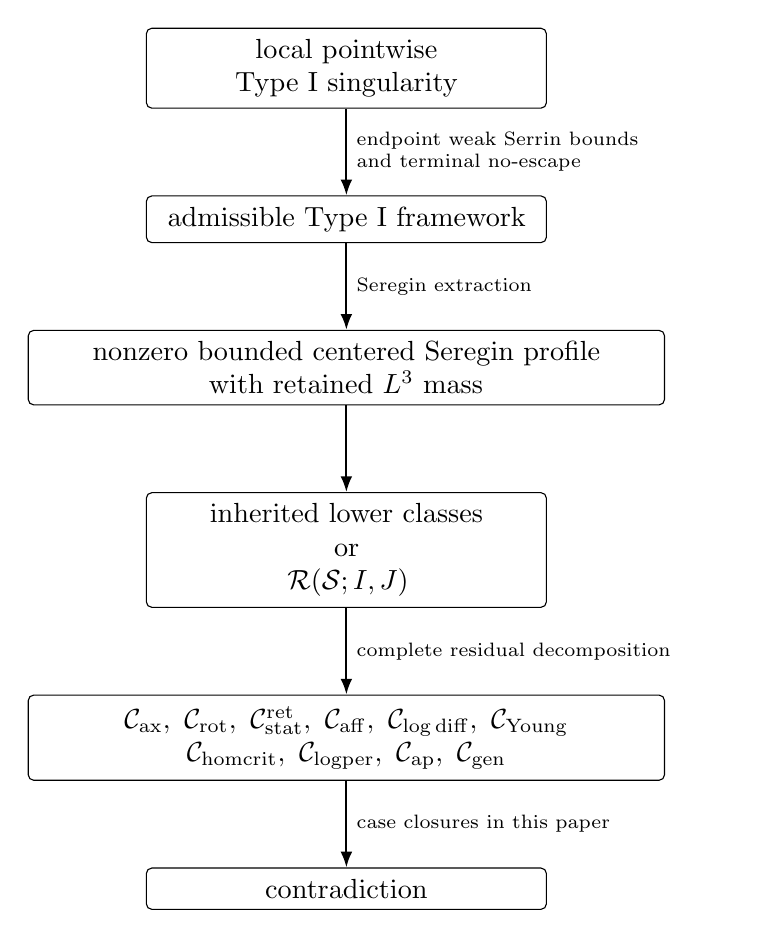
\begin{tikzpicture}[
   node distance=1.10cm,
   box/.style={draw, rounded corners=2pt, align=center, text width=4.8cm,
      inner sep=4pt},
   widebox/.style={draw, rounded corners=2pt, align=center, text width=7.8cm,
      inner sep=4pt},
   arrow/.style={-{Latex[length=2mm]}, thick},
   lab/.style={align=left, font=\scriptsize, text width=4.7cm}
]
\node[box] (typeI) {local pointwise Type~I singularity};
\node[box, below=of typeI] (admissible) {admissible Type~I framework};
\node[widebox, below=of admissible] (seregin)
   {nonzero bounded centered Seregin profile\\with retained \(L^3\) mass};
\node[box, below=of seregin] (split)
   {inherited lower classes\\or\\\(\calR(\calS;I,J)\)};
\node[widebox, below=of split] (decomp)
   {\(\Cax,\ \Crot,\ \Cstat,\ \Caff,\ \Clogdiff,\ \Cyoung\)\\
    \(\Chomcrit,\ \Clogper,\ \Capcrit,\ \Cgen\)};
\node[box, below=of decomp] (contradiction) {contradiction};

\draw[arrow] (typeI) -- node[lab, right]
   {endpoint weak Serrin bounds\\and terminal no-escape} (admissible);
\draw[arrow] (admissible) -- node[lab, right] {Seregin extraction} (seregin);
\draw[arrow] (seregin) -- (split);
\draw[arrow] (split) -- node[lab, right] {complete residual decomposition} (decomp);
\draw[arrow] (decomp) -- node[lab, right] {case closures in this paper}
   (contradiction);
\end{tikzpicture}}
\caption{Decision diagram for the Type~I state-space stratification.  The first
arrow uses the local pointwise Type~I to terminal no-escape bridge supplied by
the endpoint weak Serrin local Type~I estimate.  The inherited lower classes in
the split node are already closed in the setup paper.  The residual alternatives in the boxed
list are excluded by the case-closure theorems cited in the proof of
\Cref{thm:refined-residual-closure-complete-decomposition}.}
\label{fig:typeI-state-stratification-tree}
\end{figure}

\begin{theorem}[Admissible Type I Seregin extraction theorem]
\label{hyp:base-seregin-package}
\label{thm:base-seregin-package}
An admissible finite-energy Type I singular point produces a normalized Seregin
ancient limit \((V,P)\) satisfying \eqref{eq:centered-main}, with
\[
   \|V\|_{L^\infty(\R^3\times\R)}\le M<\infty,
\]
local suitability and local pressure-gauge compactness, and a compact
parabolic cylinder \(K\Subset\R^3\times\R\) for which
\begin{equation}\label{eq:positive-velocity-main}
   \iint_K |V|^3\,dy\,d\tau
   \ge \eta_0>0 .
\end{equation}
The collection of all normalized Seregin limits generated by the original
solution is
denoted by \(\calS\).
\end{theorem}

\begin{proof}
This is the base admissible Seregin extraction theorem from
\(\texttt{proof\_setup.tex}\), including velocity nonvanishing, local suitability,
and local pressure compactness.  The underlying positive local concentration
input is also provided there.  The present paper uses this as an inherited
reduction and does not reprove the Type I blow-up compactness theorem.
\end{proof}

\begin{definition}[Earlier alternatives inherited from the setup paper]
\label{hyp:previous-nonresidual}
Within a fixed normalized Seregin collection \(\calS\), the small-amplitude,
stationary \(L^3\), uniformly \(L^3\)-tight, and closed structured/decay
classes are the non-residual alternatives already established in the setup
paper.  The small-amplitude and stationary \(L^3\) alternatives are closed
there; the uniformly tight class is excluded there; and the closed structured/decay
class is precisely the part proved empty there.  Any structured profile not
belonging to that closed class is residual by definition and is handled by
the present paper.  The present paper does not reprove those earlier
alternatives and does not add any hypothesis to their statements.
\end{definition}

\begin{definition}[Coarse residual class]
\label{def:coarse-residual}
Let \(I,J\) be the index sets used in the base Type I residual
criterion.  The raw coarse residual class
\[
   \calR_{\rm raw}(\calS;I,J)
\]
is the complement in \(\calS\) of the already removed alternatives in
\Cref{hyp:previous-nonresidual}.  The retained normalized residual class
\[
   \calR^\#(\calS;I,J)
\]
is obtained from \(\calR_{\rm raw}(\calS;I,J)\) by passing to the canonical
affine/parasitic representative and by removing any representative assigned to
the affine/parasitic lower stratum.  Unless the word raw is used explicitly,
\(\calR(\calS;I,J)\) denotes this retained normalized residual class.  Thus an
``empty affine/parasitic stratum'' below always means that no retained
normalized residual representative remains in that quotient stratum.
\end{definition}

\begin{definition}[Refined residual decomposition]
\label{def:refined-decomposition}
The refined residual decomposition is an ordered definition, not a separate
compactness theorem.  Starting with the raw coarse residual class
\(\calR_{\rm raw}(\calS;I,J)\), one removes the following alternatives in
order; the affine/parasitic alternative is then recorded as a quotient stratum
with no retained normalized representative in \(\calR^\#(\calS;I,J)\).  After
the first nine alternatives have been removed, whatever remains is by definition
the generic terminal residual \(\Cgen\):
\[
\begin{gathered}
   \Cax,\qquad \Crot,\qquad \Cstat,\qquad \Caff,\\
   \Clogdiff,\qquad \Cyoung,\qquad
   \Chomcrit,\qquad \Clogper,\qquad \Capcrit,\qquad \Cgen .
\end{gathered}
\]
Here \(\Cax\) is the axisymmetric bounded-circulation class, \(\Crot\) is the
rotational relative-equilibrium class, \(\Cstat\) is the degenerate
stationary-hull class with retained local concentration, \(\Caff\) is the
affine/parasitic lower stratum selected by affine-normalized oscillatory entry,
\(\Clogdiff\) and \(\Cyoung\) are respectively the log-diffuse and Young
critical-tail alternatives, \(\Chomcrit,\Clogper,\Capcrit\) are the coherent
homogeneous, log-periodic, and aperiodic critical-tail alternatives, and \(\Cgen\)
is the generic terminal residual class.  The inclusion below is part of this
ordered definition, written for the retained normalized residual class; the
appearance of \(\Caff\) records the quotient alternative before retained
normalization, and \(\Caff\cap\calR^\#(\calS;I,J)=\varnothing\) is proved in
\Cref{thm:oscillatory-entry-normalization}.  The substantive content is the
closure of each non-quotient alternative, especially \(\Cgen\).  Equivalently,
\begin{equation}\label{eq:complete-residual-decomposition}
   \calR(\calS;I,J)
   \subset
   \Cax\cup\Crot\cup\Cstat\cup\Caff
   \cup\Clogdiff\cup\Cyoung\cup\Chomcrit\cup\Clogper\cup\Capcrit
   \cup\Cgen .
\end{equation}
\end{definition}

\begin{definition}[Ancestor-realized residual objects]
\label{def:ancestor-realized-residual-object}
Fix a normalized Seregin collection \(\calS\) and a retained residual candidate
\((V,P)\in\calR(\calS;I,J)\).  An auxiliary object used in the residual proof is
\emph{ancestor-realized} if it is obtained from \((V,P)\), or from the terminal
sequence which generated \((V,P)\), by a finite or diagonal sequence of the
following operations:
\begin{enumerate}[label=\textup{(\roman*)}]
   \item exact centered symmetries \(T_a\), \(\Theta_s\), and the covariant
   observer maps \(\calR_z\);
   \item raw parabolic recenterings before passing to centered variables, with
   the local pressure gauges supplied by Seregin compactness;
   \item retained tail limits or active successors with
   \(\calE_1\ge\eps_*\) after the fixed admissible pressure gauges;
   \item normalized diffuse or critical-tail defect limits obtained by
   restricting the ancestor defect measure to a positive-measure window and
   renormalizing it;
   \item minimal mesoscopic blow-downs selected from such retained or
   normalized defect windows.
\end{enumerate}
The word ``ancestor'' always refers to the original singularity-generated
candidate \((V,P)\), not merely to the immediately preceding normalized state.
\end{definition}

\begin{theorem}[Ancestor-realization and heredity principle]
\label{thm:ancestor-realization-discharge}
Every descendant, tail limit, active successor, log-window normalization,
critical-tail state, and minimal-scale blow-down used in the proof of
\Cref{thm:refined-residual-closure-complete-decomposition} is ancestor-realized in the
sense of \Cref{def:ancestor-realized-residual-object}.  More precisely, each
such object satisfies one of the following alternatives.
\begin{enumerate}[label=\textup{(\alph*)}]
   \item It is a retained Seregin descendant of the original candidate, with
   the fixed descendant lower bound \(\calE_1\ge\eps_*\).
   \item It is a normalized defect state whose unnormalized ancestor defect
   measure has positive total mass on the selected window.  If every normalized
   window descendant is excluded, then the original defect is excluded.
   \item It lies in a previously closed lower stratum, and the retained
   descendant heredity theorem applies.
   \item It generates a retained descendant or a normalized defect descendant
   satisfying \textup{(a)}, \textup{(b)}, or \textup{(c)}.
\end{enumerate}
Consequently a contradiction obtained for an ancestor-realized object is a
contradiction for the original retained residual candidate, not merely for an
auxiliary compactification state.
\end{theorem}

\begin{proof}
It suffices to verify the assertion for the operations listed in
\Cref{def:ancestor-realized-residual-object}.  Exact centered
symmetries preserve the centered equation, local suitability, pressure gauges,
and retained local concentration; this is recorded in
\Cref{lem:covariant-translation-invariance,thm:covariant-observer-calculus}.
Raw terminal recenterings before centering are the recenterings in the Seregin
extraction theorem of the setup paper and are compact after the gauges in
\Cref{prop:local-typeI-terminal-compactness}.  Retained tail limits and active
successors are ancestor-realized by diagonal lifting:
\Cref{lem:diagonal-lifting-descendants,thm:descendant-heredity} show that the
limit remains in the normalized state space and keeps the fixed retained CKN
threshold, up to the once-for-all threshold loss in
\Cref{def:threshold-hierarchy}.

Normalized defect states are obtained by restricting a positive ancestor defect
measure to a window and dividing by its mass.  The mass of the chosen window may
depend on the index and may tend to zero; this does not detach the normalized
state from the ancestor.  It records a point in the support of the ancestor
defect compactification.  The renormalized-window heredity lemma
\Cref{lem:renormalized-log-window-heredity} below states explicitly that if all
such support descendants are assigned to closed lower alternatives, then the
ancestor defect measure itself has no surviving mass outside those alternatives.

Minimal-scale blow-downs are selected from retained or normalized defect windows;
their centers and scales therefore come with the same ancestor measure or
retained CKN lower bound.  The pressure/gauge normalization for those blow-downs
is treated in
\Cref{lem:first-bad-quotient-formulation,prop:normalized-pressure-representation,lem:first-bad-pressure-compactness}.
Thus every contradiction later in the proof is applied either to a retained
descendant of the original profile or to a normalized support state whose
closure removes the corresponding ancestor defect.  This proves the stated
principle.
\end{proof}

\begin{lemma}[Contradiction transfer for ancestor-realized states]
\label{lem:ancestor-contradiction-transfer}
Let \((V,P)\in\calR(\calS;I,J)\) be a retained residual candidate, and let
\(\mathcal A\) be a closed union of lower alternatives which is stable under
the descendant operations used in this paper.  Suppose that every
ancestor-realized object generated from \((V,P)\) by the relevant construction
has one of the following two properties:
\begin{enumerate}[label=\textup{(\roman*)}]
   \item it is a retained Seregin descendant lying in \(\mathcal A\);
   \item it is a normalized support state of an ancestor defect measure and lies
   in \(\mathcal A\).
\end{enumerate}
If \(\mathcal A\) has already been excluded in the ordered residual
decomposition, then the original candidate \((V,P)\) cannot exist.
\end{lemma}

\begin{proof}
In case \textup{(i)}, retained descendant heredity
\Cref{thm:descendant-heredity} identifies the descendant as an admissible
successor of the original residual candidate with the retained threshold fixed
in \Cref{def:threshold-hierarchy}.  Since \(\mathcal A\) is closed under the
allowed state-space operations and is excluded, the retained descendant cannot
occur.

In case \textup{(ii)}, the normalized state is obtained by restricting a
positive ancestor defect measure to a window and renormalizing.  If all such
normalized support states lie in the closed excluded set \(\mathcal A\), then
regularity of the compactified defect measure implies that the ancestor defect
measure has no mass outside \(\mathcal A\); this is exactly the mechanism made
explicit for logarithmic windows in
\Cref{lem:renormalized-log-window-heredity}.  Hence the defect has no surviving
support in the residual class after \(\mathcal A\) is removed.  In both cases
the construction cannot produce a retained residual object from \((V,P)\),
contradicting the defining retained concentration of the residual candidate.
\end{proof}

\begin{theorem}[Refined residual closure for the complete ordered decomposition]
\label{thm:refined-residual-closure}
\label{thm:refined-residual-closure-complete-decomposition}
Relative to the inherited alternatives in
\Cref{hyp:base-seregin-package,hyp:previous-nonresidual}, one has
\[
\begin{gathered}
   \Cax=\Crot=\Cstat=\Cgen=\varnothing,\\
   \Clogdiff=\Cyoung=\Chomcrit=\Clogper=\Capcrit=\varnothing .
\end{gathered}
\]
Moreover,
\[
   \Caff\cap\calR^\#(\calS;I,J)=\varnothing ,
\]
that is, no retained normalized residual representative remains in the
affine/parasitic quotient stratum.  Consequently
\[
   \calR^\#(\calS;I,J)=\varnothing .
\]
\end{theorem}

\begin{proof}
This proof is the forward summary of the class closures established in the
sections below and assembled again in \Cref{sec:final-assembly}.  The
dependency order is recorded in \Cref{tab:paperIV-dependency-order}.
The axisymmetric bounded-circulation class is excluded by
\Cref{thm:R1-exclusion}.  The rotational relative-equilibrium class is excluded by
\Cref{thm:R2-exclusion-safe}, which uses the localized Coriolis-flux identity
and a terminal local concentration decomposition rather than a whole-space
Coriolis--Leray Liouville theorem.
The degenerate stationary-hull class with retained local concentration
\(\Cstat\) is excluded by \Cref{thm:R3S-R3-empty}, using the
terminal local concentration theorem proved in
\Cref{sec:terminal-concentration,sec:separated-profiles-atomic}.
The retained normalized affine/parasitic quotient stratum is removed by
\Cref{thm:oscillatory-entry-normalization}.  The log-diffuse and Young
critical-tail alternatives are excluded by
\Cref{cor:log-diffuse-branch-discharge,cor:young-branch-discharge}.
The coherent homogeneous, log-periodic, and aperiodic critical-tail alternatives are
excluded by \Cref{cor:coherent-critical-tail-branch-closure}.  Finally, the
generic terminal residual class \(\Cgen\) is excluded by
\Cref{thm:R4-final-closure}.  These ordered exclusions exhaust the complete
decomposition \eqref{eq:complete-residual-decomposition}.
\end{proof}

\begin{longtable}{@{}>{\raggedright\arraybackslash}p{0.26\textwidth}>{\raggedright\arraybackslash}p{0.68\textwidth}@{}}
\caption{Dependency order for the residual closure proof.}
\label{tab:paperIV-dependency-order}\\
\hline
\textbf{Step} & \textbf{Status and allowed dependencies}\\
\hline
\endfirsthead
\hline
\textbf{Step} & \textbf{Status and allowed dependencies}\\
\hline
\endhead
\hline
\endfoot
Base Seregin extraction &
Inherited from the setup paper.  It supplies bounded centered profiles,
local suitability, local pressure-gauge compactness, and retained compact
velocity \(L^3\)-mass.  It does not use any residual closure result from this
paper.\\
Setup lower alternatives &
The small-amplitude, stationary \(L^3\), uniformly tight, and closed
structured/decay alternatives are inherited from the setup paper and are not
reproved here.\\
Axisymmetric class &
Proved in \Cref{sec:R1-exclusion} from the centered circulation equation and
the scalar axis-absorption Liouville theorem.\\
Rotational class &
Proved in \Cref{sec:R2-reduction} from the localized Coriolis-flux identity
and local concentration recentering; no whole-space Coriolis--Leray Liouville
theorem is used.\\
Stationary-hull class &
Reduced by scale reselection and closed through the terminal concentration
theorem; it does not use the generic residual closure.\\
Affine/parasitic quotient &
Removed by canonical affine/parasitic normalization and oscillatory-entry
normalization.  This is a quotient removal statement: no retained normalized
representative remains in \(\Caff\).\\
Log-diffuse and Young alternatives &
Reduced to hidden-scale compactness and the minimal mesoscopic-scale reduction
theorem; no global critical-norm bound is used.\\
Coherent critical tails &
Excluded by bounded-origin realization and the local boundedness contradiction
for homogeneous, log-periodic, and aperiodic coherent tails.\\
Terminal concentration theorem &
Assembled from active-locus extraction, diffuse-defect trichotomy, active
path-space recurrence, mixed compact--diffuse exclusion, and finite
separated-family exclusion.  It is used before the generic residual closure.\\
Generic residual class &
Closed last, using all preceding alternatives, terminal indecomposability,
parasitic-free mildness, the sequence-\(L^3\) conclusion, and the
Albritton--Barker endpoint Liouville theorem.\\
\hline
\end{longtable}

\begin{corollary}[Residual input from the setup paper]
\label{cor:paperI-residual-input}
For every normalized Seregin collection \(\calS\) generated by an
admissible finite-energy Type I singularity in the setup paper, the setup
remaining class is empty.
\end{corollary}

\begin{proof}
The setup paper defines its remaining class as the complement, inside \(\calS\), of
the small-amplitude, stationary \(L^3\), uniformly \(L^3\)-tight, and closed
structured/decay classes.  This is the raw residual class
\(\calR_{\rm raw}(\calS;I,J)\).  Passing to the canonical affine/parasitic
representative gives the retained normalized class \(\calR^\#(\calS;I,J)\);
if the representative is assigned to \(\Caff\), it is already in a closed lower
quotient stratum.  The indices \(I,J\) add no analytic assumption.  By
\Cref{thm:refined-residual-closure}, no retained normalized residual
representative remains, and hence the setup remaining class is empty.
\end{proof}

\begin{theorem}[Local pointwise Type I exclusion after residual closure]
\label{thm:typeI-exclusion-main}
No finite-energy local pointwise Type~I singularity can generate a normalized
Seregin collection \(\calS\).
\end{theorem}

\begin{proof}
Suppose that such a singular point exists.  The setup paper supplies a
positive local velocity concentration sequence.  By
\Cref{thm:local-typeI-terminal-energy-package,cor:local-typeI-implies-admissible},
the local pointwise Type~I envelope gives the terminal velocity
no-escape condition for this sequence.  Hence
\Cref{hyp:base-seregin-package} applies, and the Seregin blow-up procedure
produces a
normalized ancient limit \((V,P)\) satisfying \eqref{eq:centered-main} and the
local velocity nonvanishing condition \eqref{eq:positive-velocity-main}.  By
the inherited class exhaustion, \(V\) is either in one of the non-residual
classes recorded in \Cref{hyp:previous-nonresidual} or in
\(\calR(\calS;I,J)\).  The first alternative is impossible by the corresponding
closed inputs: the small and stationary \(L^3\) classes are excluded in the setup
paper, the uniformly \(L^3\)-tight class is also excluded there, and the
closed structured/decay class is excluded there.  The second alternative is
impossible by \Cref{thm:refined-residual-closure}.  This contradiction proves
the theorem.
\end{proof}

\subsection{Local Type I singularities enter the terminal concentration framework}
\label{sec:local-typeI-bridge}

The purpose of this subsection is to make explicit the local reduction that is
implicit in the two-paper proof architecture here.  There are two logically
different issues.  The local pointwise Type~I envelope gives Seregin compactness
on every compact negative-time cylinder
\[
   B_R\times[-S,-\sigma],\qquad \sigma>0,
\]
but this compactness is strictly away from the terminal slice \(t=0\).  It does
not alone imply that the positive \(L^3\)-mass in
\(B_1\times(-1,0)\) survives away from the terminal layer
\((- \sigma,0)\).  The latter is exactly the terminal velocity no-escape
condition used in the setup paper.

The bridge below first records the admissible form used by the unified setup
paper.  It then uses the endpoint weak Serrin local Type~I estimate of
Albritton--Barker to derive the required scale-invariant \(L^2\) bound on the
terminal interval.  Interpolation with the Type~I envelope gives terminal
velocity no-escape.

For this subsection, if \(z_*=(x_*,T)\) and \(r_n\downarrow0\), write
\[
   u_n(x,t):=r_nu(x_*+r_nx,T+r_n^2t),
   \qquad
   p_n(x,t):=r_n^2p(x_*+r_nx,T+r_n^2t).
\]
Also write \(Q_R:=B_R(0)\times(-R^2,0)\) and
\[
   Q_1(0,0)=B_1(0)\times(-1,0).
\]

\begin{definition}[Admissible local Type I concentration sequence]
\label{def:admissible-local-typeI-sequence}
Let \(z_*=(x_*,T)\) satisfy the local Type~I bound
\eqref{eq:local-typeI-bridge-bound}, and let \(r_n\downarrow0\).  The
corresponding rescaled velocities \(u_n\) form an admissible local Type~I
concentration sequence if there are \(\eta_v>0\) such that
\begin{equation}\label{eq:admissible-local-typeI-positive-mass}
   \iint_{B_1\times(-1,0)} |u_n|^3\,dx\,dt\ge\eta_v
   \qquad\hbox{for every }n,
\end{equation}
and the terminal velocity no-escape condition holds:
\begin{equation}\label{eq:admissible-local-typeI-no-escape}
   \lim_{\sigma\downarrow0}
   \sup_n
   \iint_{B_1\times(-\sigma,0)} |u_n|^3\,dx\,dt=0 .
\end{equation}
Equivalently, after lowering the mass threshold, there are
\(\sigma_0\in(0,1)\) and \(\eta_1>0\) such that
\begin{equation}\label{eq:admissible-local-typeI-away-mass}
   \iint_{B_1\times(-1,-\sigma_0)} |u_n|^3\,dx\,dt\ge\eta_1
   \qquad\hbox{for all }n .
\end{equation}
\end{definition}

\begin{lemma}[No-escape leaves positive mass away from the terminal layer]
\label{lem:local-no-escape-away-mass}
If \(u_n\) is an admissible local Type~I concentration sequence in the sense of
\Cref{def:admissible-local-typeI-sequence}, then
\eqref{eq:admissible-local-typeI-away-mass} holds for some
\(\sigma_0\in(0,1)\) and some \(\eta_1>0\).
\end{lemma}

\begin{proof}
Choose \(\sigma_0\in(0,1)\) so small that
\[
   \sup_n
   \iint_{B_1\times(-\sigma_0,0)} |u_n|^3\,dx\,dt
   \le \frac12\eta_v ,
\]
which is possible by \eqref{eq:admissible-local-typeI-no-escape}.  Subtracting
this terminal-layer contribution from
\eqref{eq:admissible-local-typeI-positive-mass} gives
\[
   \iint_{B_1\times(-1,-\sigma_0)} |u_n|^3\,dx\,dt
   \ge \frac12\eta_v .
\]
Take \(\eta_1=\eta_v/2\).
\end{proof}

\begin{proposition}[Local Type I rescalings have Seregin compactness]
\label{prop:local-typeI-terminal-compactness}
Let \((u,p)\) be a suitable Leray--Hopf solution on
\(\R^3\times(0,T)\), let \(z_*=(x_*,T)\) be a singular point, and assume that
there exist \(\rho>0\) and \(M<\infty\) such that
\begin{equation}\label{eq:local-typeI-bridge-bound}
   \esssup_{T-\rho^2<t<T}
   \sqrt{T-t}\,\|u(t)\|_{L^\infty(B_\rho(x_*))}\le M .
\end{equation}
Let \(r_n\downarrow0\), and let \((u_n,p_n)\) be the rescaled sequence above.
Then the following hold.
\begin{enumerate}[label=\textup{(\roman*)}]
\item For every compact cylinder
\[
   K=B_R\times[-S,-\sigma]\Subset\R^3\times(-\infty,0),
   \qquad R,S<\infty,\quad \sigma>0,
\]
there exists \(n_0(K)\) such that
\begin{equation}\label{eq:local-typeI-bridge-unifLinfty}
   \|u_n\|_{L^\infty(K)}\le M\sigma^{-1/2},
   \qquad n\ge n_0(K).
\end{equation}
\item On every compact cylinder \(K\Subset\R^3\times(-\infty,0)\) there are
time-dependent pressure gauges \(a_{n,K}(t)\) and a constant \(C_K<\infty\)
such that, for \(n\ge n_0(K)\),
\begin{equation}\label{eq:local-typeI-bridge-local-bounds}
   \|u_n\|_{L^\infty_tL^2_x(K)}
   +\|\nabla u_n\|_{L^2(K)}
   +\|p_n-a_{n,K}(t)\|_{L^{3/2}(K)}
   \le C_K .
\end{equation}
The constant \(C_K\) may depend on the fixed Leray energy level of the original
solution, but no concentration or no-escape assumption enters it.
\item After subtracting these local pressure gauges, the family
\((u_n,p_n)\) is locally precompact in the standard Seregin topology on
\(\R^3\times(-\infty,0)\).  Along every subsequence there is a further
subsequence and an ancient suitable weak solution \((U,Q)\) such that, on
every compact \(K\Subset\R^3\times(-\infty,0)\),
\[
   u_n\to U\quad\hbox{strongly in }L^q(K),\qquad 1\le q<\infty,
\]
and
\[
   p_n-a_{n,K}(t)\rightharpoonup Q
   \quad\hbox{weakly in }L^{3/2}(K).
\]
The limit is bounded and satisfies
\[
   |U(x,t)|\le M(-t)^{-1/2},\qquad t<0.
\]
\item More generally, let \(\mathfrak c=(z_n)\), \(z_n=(y_n,\tau_n)\), be a
parabolic recentering sequence for \((u_n,p_n)\) with \(\tau_n\le0\).  Assume
that \(\mathfrak c\) remains in the local Type~I window in the following
precise sense: for every \(R,S<\infty\), all sufficiently large \(n\) satisfy
\[
   r_n(|y_n|+R)<\rho,
   \qquad
   T+r_n^2(\tau_n-S)>T-\rho^2 .
\]
If \(\mathfrak c\) carries retained compact velocity \(L^3\)-mass, then after
passing to a subsequence it has no loss of local compactness in the sense of
\Cref{def:terminal-measures}, and its recentered fields converge locally to a
bounded suitable terminal profile.  Recenterings which do not satisfy this
local-window condition are, by definition, assigned to the exterior or diffuse
terminal alternatives rather than to the compact local profile class.
\end{enumerate}
\end{proposition}

\begin{proof}
Fix
\[
   K=B_R\times[-S,-\sigma]\Subset\R^3\times(-\infty,0).
\]
For \(n\) sufficiently large,
\[
   r_nR<\rho/2,\qquad r_n^2S<\rho^2/2.
\]
Hence, for a.e. \((x,t)\in K\),
\[
   x_*+r_nx\in B_\rho(x_*),
   \qquad
   T+r_n^2t\in(T-\rho^2,T).
\]
The local Type~I bound \eqref{eq:local-typeI-bridge-bound} gives
\[
   |u_n(x,t)|
   =r_n|u(x_*+r_nx,T+r_n^2t)|
   \le r_n M\,(T-(T+r_n^2t))^{-1/2}
   =M(-t)^{-1/2}
   \le M\sigma^{-1/2}.
\]
This proves \eqref{eq:local-typeI-bridge-unifLinfty}.  In particular,
\[
   \esssup_{-S<t<-\sigma}\int_{B_R}|u_n(x,t)|^2\,dx
   \le |B_R|M^2\sigma^{-1},
\]
and
\[
   \iint_K |u_n|^3\,dx\,dt
   \le |K|M^3\sigma^{-3/2}.
\]

We next record the pressure estimate, where the nonlocal pressure contribution
is localized in the local Type~I compactness argument.  We use the whole-space
Leray pressure representative, so at each rescaled time
\[
   p_n(\cdot,t)=\mathcal R_i\mathcal R_j
      \bigl(u_{n,i}u_{n,j}\bigr)(\cdot,t)
\]
modulo a function of time.  Fix a cutoff
\(\chi_R\in C_c^\infty(B_{8R})\) with \(\chi_R\equiv1\) on \(B_{4R}\), and
write in \(B_{4R}\)
\[
   p_n=q_n+h_n,\qquad
   q_n=\mathcal R_i\mathcal R_j(\chi_R u_{n,i}u_{n,j}).
\]
The local term satisfies
\[
   \|q_n\|_{L^{3/2}(B_{4R}\times[-S,-\sigma])}
   \le C_{R,S,\sigma,M}.
\]
For the harmonic part choose the gauge \(a_{n,K}(t)=h_n(0,t)\).  The standard
kernel difference estimate for the Riesz pressure kernel is as follows.  If
\[
   K_{ij}(x)=c_3\,\mathrm{p.v.}\,
      \frac{3x_ix_j-\delta_{ij}|x|^2}{|x|^5}
\]
is the Calder\'on--Zygmund pressure kernel, then for \(|x|\le2R\) and
\(|z|\ge4R\),
\[
   |K_{ij}(x-z)-K_{ij}(-z)|\le C_R|z|^{-4}.
\]
Decomposing the exterior region into dyadic annuli gives, for \(x\in B_{2R}\),
\[
   |h_n(x,t)-a_{n,K}(t)|
   \le
   C_R\sum_{m\ge2}2^{-4m}
   \int_{2^mR<|z|<2^{m+1}R}|u_n(z,t)|^2\,dz .
\]
For annuli whose physical image remains in \(B_\rho(x_*)\), namely while
\(2^{m+1}Rr_n\le\rho\), the local Type~I bound and \(-t\ge\sigma\) on \(K\)
give
\[
   \int_{2^mR<|z|<2^{m+1}R}|u_n(z,t)|^2\,dz
   \le C M^2\sigma^{-1}(2^mR)^3 .
\]
Multiplication by \(2^{-4m}\) leaves a summable \(2^{-m}\) factor, so the
corresponding part of the series is bounded by a geometric sum depending only
on \(R,M,\sigma\).  For the remaining outer annuli one uses only the finite
Leray energy of the original solution:
\[
   \int_{\R^3}|u_n(z,t)|^2\,dz
   =r_n^{-1}\int_{\R^3}|u(y,T+r_n^2t)|^2\,dy .
\]
If \(m_n\) is the first index for which \(2^{m_n}Rr_n\gtrsim\rho\), then
\[
   \sum_{m\ge m_n}2^{-4m}\int_{\R^3}|u_n(z,t)|^2\,dz
   \le
   C_{\rho,R}\,r_n^3\|u\|_{L^\infty(0,T;L^2)}^2
   \le C_{\rho,R,u}.
\]
Thus \(h_n-a_{n,K}\) is uniformly bounded on
\(B_{2R}\times[-S,-\sigma]\).  Since this cylinder has finite measure,
\[
   \|h_n-a_{n,K}\|_{L^{3/2}(B_{2R}\times[-S,-\sigma])}
   \le C_K .
\]
Together with the Calder\'on--Zygmund bound for \(q_n\), this gives
\[
   \|p_n-a_{n,K}(t)\|_{L^{3/2}(B_{2R}\times[-S,-\sigma])}
   \le C_K .
\]

Apply the local energy inequality for \((u_n,p_n)\) with a cutoff equal to one
on \(K\) and supported in a slightly larger compact cylinder
\(K'\Subset\R^3\times(-\infty,0)\).  The already obtained local \(L^2\),
\(L^3\), and pressure-gauge bounds control every term on the right-hand side,
and therefore
\[
   \iint_K |\nabla u_n|^2\,dx\,dt\le C_K .
\]
This proves \eqref{eq:local-typeI-bridge-local-bounds}.

The Navier--Stokes equation now bounds \(\partial_tu_n\) locally in a negative
Sobolev space, for instance in \(L^{3/2}_tH^{-2}_x(K)\).  Aubin--Lions
compactness and the uniform \(L^\infty\) bound give strong local convergence of
the velocity in every finite \(L^q\), after passing to a subsequence.  The
pressure bound gives weak \(L^{3/2}\) convergence after gauges.  Passing to the
limit in the distributional equations and in the local energy inequality gives
an ancient suitable weak solution \((U,Q)\).  The pointwise Type~I bound passes
to the limit, so \(U\) is bounded on every compact negative-time cylinder.
This proves (iii).

Finally, let \(\mathfrak c=(y_n,\tau_n)\) be as in (iv), and set
\[
   u_n^{\mathfrak c}(y,s)=u_n(y+y_n,s+\tau_n),
   \qquad
   p_n^{\mathfrak c}(y,s)=p_n(y+y_n,s+\tau_n).
\]
The local-window condition, together with \(\tau_n\le0\), is exactly what is
needed to repeat the preceding estimates on each fixed backward compact cylinder
in the \((y,s)\)-variables: the
physical cylinders remain in \(B_\rho(x_*)\times(T-\rho^2,T)\), the local
Type~I envelope gives the same \(L^\infty\) bound on compact windows, and the
pressure decomposition has the same local and finite-energy tail estimates.
Thus the two failure modes in \Cref{def:terminal-measures}, blow-up of the
local dissipation measure or failure of local pressure-gauge control, cannot
occur for such a retained local recentering sequence after subsequence
extraction.  The recentered fields therefore converge locally to a bounded
suitable terminal profile.  If the local-window condition fails, then the
recentering leaves every bounded terminal window attached to the singular
point, or its critical mass persists only through expanding regions; those are
precisely the exterior and diffuse terminal alternatives rather than loss of
local compactness inside the local Type~I bridge.
\end{proof}

\subsection{Pressure-projected terminal energy estimate}
\label{subsec:pressure-projected-terminal-gap}

The preceding compactness result is stated away from the terminal
slice.  The next estimate supplies the terminal-layer bound required for
velocity no-escape.  The local pressure projection removes the nonlocal pressure
flux from the local energy inequality; the remaining estimate is an interior
Caccioppoli propagation bound on balls contained in the local Type~I window.

Let \(v=u^{(r)}\), \(\pi=p^{(r)}\), and
\(\Lambda=\rho/r\).  After translating \(z_*\) to \((0,0)\), the local Type~I
bound gives
\[
   |v(x,s)|\le M(-s)^{-1/2}
   \qquad (x,s)\in B_\Lambda\times(-4,0),
\]
for all sufficiently small \(r\).  For \(a\in\mathbb R^3\), \(L\ge1\), and
\(-4<s<t<0\), write
\[
   A_L(a,s):=\int_{B_L(a)}|v(x,s)|^2\,dx,\qquad
   D_L(a;s,t):=\int_s^t\int_{B_L(a)}|\nabla v|^2\,dx\,d\sigma .
\]

\begin{lemma}[Local pressure-projected Caccioppoli inequality]
\label{lem:local-pressure-projected-caccioppoli}
There is a universal constant \(C\) with the following property.  Let
\((v,\pi)\) be a suitable weak solution in
\(B_{8L}(a)\times(s_-,0)\), \(L\ge1\), and assume
\[
   |v(x,s)|\le M(-s)^{-1/2}
   \qquad\hbox{on }B_{8L}(a)\times(s_-,0).
\]
If \(s_0\in(s_-,0)\) is a Lebesgue time for \(v\) and \(\nabla v\), then for
a.e. \(t\in(s_0,0)\),
\begin{equation}\label{eq:pressure-projected-caccioppoli}
\begin{aligned}
   \int_{B_L(a)}|w(x,t)|^2\,dx+D_L(a;s_0,t)
   &\le
   C A_{4L}(a,s_0)                                      \\
   &\quad
   +C\int_{s_0}^{t}
      \left(L^{-2}+ML^{-1}(-s)^{-1/2}\right)
      A_{4L}(a,s)\,ds .
\end{aligned}
\end{equation}
The estimate is entirely local on \(B_{8L}(a)\); no pressure tail from outside
\(B_{8L}(a)\) appears.  Here \(w=v+\nabla p_h\) is the local projected velocity
defined in the proof below.
\end{lemma}

\begin{proof}
The proof uses the standard local pressure-projection argument in the scale \(L\)
normalization.  Let \(B=B_{8L}(a)\).  Denote by \(E_B^*\) the Stokes pressure
projection on \(B\): for \(F\in W^{-1,q}(B)\), \(1<q<\infty\),
\(\nabla E_B^*(F)\) is the gradient part of the stationary Stokes solution in
\(B\) with zero boundary velocity.  It satisfies the scale-invariant estimates
\[
   \|\nabla E_B^*(\nabla\cdot F)\|_{L^q(B)}
   \le C_q\|F\|_{L^q(B)},\qquad
   \|\nabla E_B^*(\Delta w)\|_{L^2(B)}
   \le C\|\nabla w\|_{L^2(B)}.
\]
Set
\[
   \nabla p_h=-\nabla E_B^*(v),\qquad
   w:=v+\nabla p_h .
\]
The harmonic pressure \(p_h\) is harmonic in \(B\), and the projection estimates
give
\[
   \|w\|_{L^2(B)}+\|\nabla p_h\|_{L^2(B)}
   \le C\|v\|_{L^2(B)},\qquad
   \|\nabla w\|_{L^2(B_{6L}(a))}
   \le C\|\nabla v\|_{L^2(B)} .
\]
The projected local energy inequality for \(w\), obtained by applying the
Stokes projection to the distributional Navier--Stokes equations and testing
with \(\zeta^2 w\), reads
\begin{align}
   &\int |w(t)|^2\zeta^2
      +\int_{s_0}^{t}\int |\nabla v|^2\zeta^2              \notag\\
   &\qquad\le
      C\int |w(s_0)|^2\zeta^2
      +C\int_{s_0}^{t}\int |w|^2
        \left(|\partial_s\zeta|+|\Delta\zeta|+|\nabla\zeta|^2\right)
                                                                  \notag\\
   &\qquad\quad
      +C\int_{s_0}^{t}\int |v|\,|w|^2\,|\nabla\zeta|
      +C\int_{s_0}^{t}\int |v|\,|\nabla p_h|^2\,|\nabla\zeta| .
\label{eq:projected-local-energy}
\end{align}
Here \(\zeta\in C_c^\infty(B_{4L}(a))\), \(\zeta\equiv1\) on \(B_L(a)\), and
\[
   |\nabla\zeta|\le CL^{-1},\qquad
   |\Delta\zeta|+|\partial_s\zeta|\le CL^{-2}.
\]
The pressure-projection estimates allow \(w\) and \(\nabla p_h\) to be bounded
by \(v\) in \(L^2(B_{4L}(a))\).  Therefore the cutoff terms in
\eqref{eq:projected-local-energy} are bounded by
\[
   C L^{-2}\int_{s_0}^{t}A_{4L}(a,s)\,ds .
\]
The two convective terms are bounded, using the Type~I envelope, by
\[
   C L^{-1}\int_{s_0}^{t}
      \|v(s)\|_{L^\infty(B_{4L}(a))}A_{4L}(a,s)\,ds
   \le
   CML^{-1}\int_{s_0}^{t}(-s)^{-1/2}A_{4L}(a,s)\,ds .
\]
The initial projected energy is controlled by
\[
   \int |w(s_0)|^2\zeta^2\,dx
   \le C A_{4L}(a,s_0).
\]
Combining the preceding bounds gives
\eqref{eq:pressure-projected-caccioppoli}.
\end{proof}

\begin{definition}[Interior terminal energy estimate]
\label{def:interior-shielding-estimate}
The local pointwise Type~I window at \(z_*\) is said to satisfy the interior
terminal energy estimate if, for every fixed \(R<\infty\), there are
\[
   r_R>0,\qquad B_R<\infty,
\]
such that every rescaling \(v=u^{(r)}\), \(0<r<r_R\), with
\(\Lambda=\rho/r\), satisfies
\begin{equation}\label{eq:interior-shielding-estimate}
   \esssup_{-1<s<0}\int_{B_{8R}}|v(x,s)|^2\,dx
   +\int_{-1}^{0}\int_{B_{8R}}|\nabla v|^2\,dx\,ds
   \le B_R .
\end{equation}
Equivalently, the dependence on \(A_{4L}\) in
\Cref{lem:local-pressure-projected-caccioppoli} can be stopped inside a fixed
multiple of the target ball, uniformly as the boundary
\(\partial B_{\rho/r}\) of the local Type~I window recedes to infinity.
\end{definition}

\begin{proposition}[Pressure-projected reduction to an interior energy bound]
\label{prop:pressure-projection-reduces-to-shielding}
Assume the local pointwise Type~I bound \eqref{eq:local-typeI-bridge-bound} at
\(z_*\).  If the interior energy estimate
\eqref{eq:interior-shielding-estimate} holds with \(R=1\), then the velocity
no-escape condition \eqref{eq:admissible-local-typeI-no-escape} holds for every
positive local Type~I concentration sequence at \(z_*\).  Consequently such a
sequence is admissible in the sense of
\Cref{def:admissible-local-typeI-sequence}.
\end{proposition}

\begin{proof}
Let \(u_n=u^{(r_n)}\) be any positive local Type~I concentration sequence.  By
\eqref{eq:interior-shielding-estimate} with \(R=1\), after discarding finitely
many indices,
\[
   \esssup_{-1<s<0}\int_{B_1}|u_n(x,s)|^2\,dx\le B_1 .
\]
The local Type~I envelope gives
\[
   \|u_n(s)\|_{L^\infty(B_1)}\le M(-s)^{-1/2}.
\]
Therefore, for \(0<\sigma<1\),
\[
\begin{aligned}
   \int_{-\sigma}^{0}\int_{B_1}|u_n|^3\,dx\,ds
   &\le
   \int_{-\sigma}^{0}
      \|u_n(s)\|_{L^\infty(B_1)}
      \int_{B_1}|u_n(x,s)|^2\,dx\,ds    \\
   &\le
   2MB_1\sigma^{1/2}.
\end{aligned}
\]
The finitely many discarded indices have absolutely continuous
\(|u_n|^3\)-integrals on \(B_1\times(-1,0)\), so taking the supremum over the
whole sequence and then letting \(\sigma\downarrow0\) gives
\eqref{eq:admissible-local-typeI-no-escape}.  The positive \(Q_1\) mass
hypothesis is the other part of
\Cref{def:admissible-local-typeI-sequence}.
\end{proof}

\begin{remark}[Pressure-projected reduction]
\label{rem:narrowed-final-bridge}
\Cref{lem:local-pressure-projected-caccioppoli} shows, independently of the
Albritton--Barker endpoint input used below, that terminal no-escape reduces
to an interior terminal energy estimate: after local pressure projection, the local
energy inequality controls the projected velocity and the dissipation up to the
larger-scale quantity \(A_{4L}\).  The estimate
\eqref{eq:interior-shielding-estimate} prevents
terminal-layer concentration entering from the boundary of the local Type~I
window.  In the present paper this bound is supplied
instead by the endpoint weak Serrin local Type~I bounds in
\Cref{thm:AB-weak-serrin-typeI-package}.
\end{remark}

\begin{theorem}[Albritton--Barker weak Serrin local Type I bounds]
\label{thm:AB-weak-serrin-typeI-package}
Let \((v,q)\) be a suitable weak solution in a parabolic cylinder
\[
   Q_\rho(z_0)=B_\rho(x_0)\times(t_0-\rho^2,t_0).
\]
Assume
\[
   v\in L^{q,\infty}_tL^{p,\infty}_x(Q_\rho(z_0)),
   \qquad
   3\le p\le\infty,\quad 2\le q\le\infty,\quad
   \frac3p+\frac2q=1 .
\]
Then for every \(0<\theta<1\), the scale-invariant local Type~I bounds are
finite on \(Q_{\theta\rho}(z_0)\): there is
\[
   K_{\theta}<\infty
\]
such that every cylinder \(Q_\lambda(y,\tau)\subset Q_{\theta\rho}(z_0)\)
satisfies
\[
   A(Q_\lambda(y,\tau))+C(Q_\lambda(y,\tau))
   +D(Q_\lambda(y,\tau))+E(Q_\lambda(y,\tau))\le K_{\theta}.
\]
Here
\[
   A(Q_\lambda(y,\tau))
   :=
   \lambda^{-1}
   \esssup_{\tau-\lambda^2<s<\tau}
   \int_{B_\lambda(y)}|v(x,s)|^2\,dx ,
\]
and \(C,D,E\) denote the usual scale-invariant \(L^3\)-velocity,
\(L^{3/2}\)-pressure, and dissipation quantities of
Albritton--Barker.  In the endpoint \(p=\infty,q=2\), the constant is allowed
to depend on the local suitable-solution background quantities on
\(Q_\rho(z_0)\), including the local \(C\)- and \(D\)-bounds.
\end{theorem}

\begin{proof}
After translating and scaling to the unit cylinder, this is Lemma~2.5 of
Albritton--Barker \cite{AlbrittonBarker2019}.  Their proof combines the weak
Serrin bound with critical Morrey estimates for suitable weak solutions.  The
endpoint \(p=\infty,q=2\) is included in the weak Serrin lemma; as emphasized
there, the resulting local Type~I bound is a suitable-solution estimate and its
constant may depend on the background local energy quantities on the larger
cylinder.
\end{proof}

\begin{theorem}[Local pointwise Type I implies terminal no-escape]
\label{thm:local-typeI-terminal-energy-package}
Let \((u,p)\) be a suitable Leray--Hopf solution on
\(\mathbb R^3\times(0,T)\), let \(z_*=(x_*,T)\), and assume that
\[
  u\in L^\infty(0,T;L^2(\mathbb R^3))
  \cap L^2(0,T;\dot H^1(\mathbb R^3)).
\]
Assume that \(z_*\) satisfies the local pointwise Type~I bound: there are
\(\rho>0\) and \(M<\infty\) such that
\begin{equation}\label{eq:local-typeI-terminal-noescape-assumption}
  \esssup_{T-\rho^2<t<T}
  \sqrt{T-t}\,\|u(t)\|_{L^\infty(B_\rho(x_*))}
  \le M .
\end{equation}
For \(0<r<\rho\), set
\[
  u^{(r)}(x,s)
  =
  r\,u(x_*+rx,T+r^2s),
  \qquad
  p^{(r)}(x,s)
  =
  r^2p(x_*+rx,T+r^2s).
\]
Then for every \(0<R<\infty\) there are constants
\[
  r_R\in(0,\rho/R),\qquad B_R<\infty,
\]
and time-dependent pressure gauges \(a_{r,R}(s)\), depending on
\(R,M,\rho,T\) and the local suitable-solution background quantities of
\((u,p)\) in \(Q_\rho(z_*)\), such that the following terminal local energy
estimate holds for every \(0<r<r_R\):
\begin{equation}\label{eq:local-terminal-energy-package}
\begin{aligned}
  &\esssup_{-1<s<0}\int_{B_R}|u^{(r)}(x,s)|^2\,dx
  +\int_{-1}^{0}\int_{B_R}|\nabla u^{(r)}|^2\,dx\,ds  \\
  &\qquad
  +\int_{-1}^{0}\int_{B_R}
      |p^{(r)}(x,s)-a_{r,R}(s)|^{3/2}\,dx\,ds
  \le B_R .
\end{aligned}
\end{equation}
Consequently, for every \(0<\sigma<1\) and every \(0<r<r_R\),
\begin{equation}\label{eq:local-terminal-noescape-bound}
  \int_{-\sigma}^{0}\int_{B_R}|u^{(r)}(x,s)|^3\,dx\,ds
  \le
  2MB_R\sigma^{1/2},
\end{equation}
and in particular
\begin{equation}\label{eq:local-terminal-noescape}
  \lim_{\sigma\downarrow0}
  \sup_{0<r<r_R}
  \int_{-\sigma}^{0}\int_{B_R}|u^{(r)}(x,s)|^3\,dx\,ds
  =0 .
\end{equation}
\end{theorem}

\begin{proof}
Fix once and for all \(0<\theta<1\), for instance \(\theta=1/2\), and put
\(L_R:=\max\{R,1\}\).  By decreasing \(r_R\), we may assume
\[
   B_{L_Rr}(x_*)\times(T-L_R^2r^2,T)\subset Q_{\theta\rho}(z_*)
   \qquad (0<r<r_R).
\]
The pointwise Type~I bound implies the endpoint weak Serrin estimate on
\(Q_\rho(z_*)\).  Indeed, after writing
\[
   f(t)=\|u(t)\|_{L^\infty(B_\rho(x_*))},
\]
one has
\[
   |\{t\in(T-\rho^2,T): f(t)>\alpha\}|
   \le M^2\alpha^{-2},
   \qquad \alpha>0,
\]
and therefore \(u\in L^{2,\infty}_tL^\infty_x(Q_\rho(z_*))\).  Applying
\Cref{thm:AB-weak-serrin-typeI-package} gives a finite constant \(K_\theta\)
such that \(A,C,D,E\le K_\theta\) on all cylinders contained in
\(Q_{\theta\rho}(z_*)\).

Taking the cylinder \(Q_{L_Rr}(z_*)\) gives
\[
   (L_Rr)^{-1}
   \esssup_{T-L_R^2r^2<t<T}
      \int_{B_{L_Rr}(x_*)}|u(x,t)|^2\,dx
   \le K_\theta ,
\]
and similarly the \(D\)- and \(E\)-bounds give
\[
   (L_Rr)^{-1}\int_{T-L_R^2r^2}^{T}
      \int_{B_{L_Rr}(x_*)}|\nabla u|^2\,dx\,dt
   \le K_\theta ,
\]
\[
   (L_Rr)^{-2}\int_{T-L_R^2r^2}^{T}
      \int_{B_{L_Rr}(x_*)}|p-a_{r,R}^{\rm phys}(t)|^{3/2}\,dx\,dt
   \le K_\theta
\]
for suitable time-dependent pressure gauges \(a_{r,R}^{\rm phys}(t)\).  Scaling
these three estimates and restricting to
\[
   B_R\times(-1,0)\subset B_{L_R}\times(-L_R^2,0)
\]
gives \eqref{eq:local-terminal-energy-package} with
\[
   a_{r,R}(s):=r^2a_{r,R}^{\rm phys}(T+r^2s),
\]
after enlarging the constant \(B_R\) by a harmless factor depending on \(R\)
and \(K_\theta\).

After translating \((x_*,T)\) to \((0,0)\), the rescaled fields also satisfy
\[
   |u^{(r)}(x,s)|\le M(-s)^{-1/2}
   \qquad (x,s)\in B_R\times(-1,0)
\]
for all \(r<r_R\), after decreasing \(r_R\) if necessary.  The terminal local
energy estimate established above gives
\[
   \esssup_{-1<s<0}\int_{B_R}|u^{(r)}(x,s)|^2\,dx\le B_R .
\]

For \(0<\sigma<1\), the local Type~I bound above and the kinetic bound give
\[
\begin{aligned}
  \int_{-\sigma}^{0}\int_{B_R}|u^{(r)}|^3\,dx\,ds
  &\le
  \int_{-\sigma}^{0}
     \|u^{(r)}(s)\|_{L^\infty(B_R)}
     \int_{B_R}|u^{(r)}(x,s)|^2\,dx\,ds  \\
  &\le
  MB_R\int_{-\sigma}^{0}(-s)^{-1/2}\,ds
  =
  2MB_R\sigma^{1/2}.
\end{aligned}
\]
This proves \eqref{eq:local-terminal-noescape-bound} and
\eqref{eq:local-terminal-noescape}.
\end{proof}

\begin{corollary}[No diffuse terminal-layer mass]
\label{cor:no-diffuse-terminal-layer-mass}
Under the hypotheses of \Cref{thm:local-typeI-terminal-energy-package}, for
every fixed \(R<\infty\) there do not exist \(r_n\downarrow0\),
\(\sigma_n\downarrow0\), and \(\varepsilon_0>0\) such that
\[
  r_n^{-2}
  \int_{T-\sigma_n r_n^2}^{T}
  \int_{B_{Rr_n}(x_*)}|u(x,t)|^3\,dx\,dt
  \ge \varepsilon_0
  \qquad\hbox{for all }n .
\]
\end{corollary}

\begin{proof}
For \(u_n=u^{(r_n)}\), the left hand side is
\[
   \int_{-\sigma_n}^{0}\int_{B_R}|u_n(x,s)|^3\,dx\,ds .
\]
By \eqref{eq:local-terminal-noescape-bound}, this is bounded by
\[
   2MB_R\sigma_n^{1/2}\to0,
\]
which contradicts any fixed positive lower bound.
\end{proof}

\begin{corollary}[Local pointwise Type I concentration sequences are admissible]
\label{cor:local-typeI-implies-admissible}
Let \((u,p)\) and \(z_*=(x_*,T)\) satisfy the hypotheses of
\Cref{thm:local-typeI-terminal-energy-package}.  Let \(r_n\downarrow0\) be any
velocity concentration sequence satisfying
\[
   \iint_{B_1\times(-1,0)} |u_n|^3\,dx\,dt\ge\eta_v>0,
   \qquad
   u_n(x,t)=r_nu(x_*+r_nx,T+r_n^2t).
\]
Then \(u_n\) is an admissible local Type~I concentration sequence in the sense
of \Cref{def:admissible-local-typeI-sequence}.
\end{corollary}

\begin{proof}
Apply \Cref{thm:local-typeI-terminal-energy-package} with \(R=1\).  After
discarding finitely many \(n\), all \(r_n<r_1\), and
\[
   \lim_{\sigma\downarrow0}
   \sup_n
   \int_{-\sigma}^{0}\int_{B_1}|u_n|^3\,dx\,dt=0 .
\]
The finitely many discarded indices do not affect the limit as
\(\sigma\downarrow0\), because each fixed suitable weak solution has
\(|u_n|^3\in L^1(B_1\times(-1,0))\).  The positive mass hypothesis is the other
condition in \Cref{def:admissible-local-typeI-sequence}.
\end{proof}

\begin{lemma}[Local Type I concentration enters the terminal dichotomy]
\label{lem:local-typeI-into-terminal-dichotomy}
Under the hypotheses of
\Cref{prop:local-typeI-terminal-compactness}, let \(r_n\downarrow0\) be a
velocity concentration sequence at \(z_*\) satisfying
\[
   \iint_{B_1\times(-1,0)} |u_n|^3\,dx\,dt\ge\eta_v>0 .
\]
Then \(r_n\) is admissible by \Cref{cor:local-typeI-implies-admissible}.  Let
\(\sigma_0,\eta_1\) be given by
\Cref{lem:local-no-escape-away-mass}.
For the associated terminal extraction sequence \((V_N,P_N)\) generated by a
Seregin limit of this sequence, choose the small-data threshold
\(\eps_{\rm sd}\le\eta_1/2\).  Then the origin extraction produces a bounded
ancient Seregin profile with retained compact local velocity mass away from the
terminal layer.  In particular the retained compact concentration generated
from the origin recentering has no loss of local compactness.  Any retained
local recentering which stays in the local Type~I window has the same compactness
property by \Cref{prop:local-typeI-terminal-compactness}; any concentration
leaving that window is assigned to the exterior or diffuse terminal remainder.
The paired terminal decomposition of \Cref{thm:terminal-exhaustion-main},
together with the mixed-state exclusions and active descendant-chain exclusions
\Cref{thm:no-mixed-compact-diffuse,thm:compact-active-descendant}, reduces the
retained possibilities to a single retained concentrating terminal profile or a
finite separated family of retained concentrating terminal profiles.
\end{lemma}

\begin{proof}
By \Cref{lem:local-no-escape-away-mass},
\[
   \iint_{B_1\times(-1,-\sigma_0)} |u_n|^3\,dx\,dt\ge\eta_1
   \qquad\hbox{for all }n .
\]
The cylinder \(B_1\times[-1,-\sigma_0]\) is compactly contained in
\(\mathbb R^3\times(-\infty,0)\).  Therefore
\Cref{prop:local-typeI-terminal-compactness} gives, after passing to a
subsequence, strong local \(L^3\) convergence on this cylinder:
\[
   u_n\to U
   \qquad\hbox{in }L^3(B_1\times(-1,-\sigma_0)).
\]
Consequently
\[
   \iint_{B_1\times(-1,-\sigma_0)} |U|^3\,dx\,dt\ge\eta_1 .
\]
Cover \(B_1\times(-1,-\sigma_0)\) by finitely many unit terminal cylinders
strictly away from \(t=0\).  At least one such cylinder carries a fixed positive
velocity lower bound, and since the local CKN measure dominates the velocity
part, choosing \(\eps_{\rm sd}\le\eta_1/2\) after adjusting by this finite cover
makes the corresponding origin-frame recentering \(\eps_{\rm sd}\)-concentrating.
This argument is precisely where no-escape is used: without
\eqref{eq:admissible-local-typeI-no-escape}, the lower bound could remain
entirely in \(B_1\times(-\sigma,0)\) for every fixed \(\sigma>0\).

The distinguished recentering satisfies the local-window condition in
\Cref{prop:local-typeI-terminal-compactness}, so it is not in the
local-compactness-failure class.  Other retained local recenterings inside the
same Type~I window have the same compactness.  Recenterings leaving the window
are exterior or diffuse terminal remainders.  The paired decomposition
\Cref{thm:terminal-exhaustion-main} records these remainders alongside the active
profile locus rather than treating them as mutually exclusive alternatives.  The
sole-carrier radiative cases are excluded by
\Cref{thm:terminal-nonactive-discharge}, mixed compact--diffuse or
compact--noncompact coexistence is excluded by
\Cref{thm:no-mixed-compact-diffuse}, and infinite active descendant chains are excluded
by \Cref{thm:compact-active-descendant}.  Hence
\Cref{cor:persistent-forces-active} leaves only a single retained concentrating
terminal profile or a finite separated family of retained concentrating terminal
profiles.
\end{proof}

\begin{theorem}[Local Type I singularities enter the exclusion argument]
\label{thm:local-typeI-entry-or-discharge}
Let \((u,p)\) be a suitable Leray--Hopf solution on
\(\R^3\times(0,T)\), let \(z_*=(x_*,T)\) be a singular point, and assume that
\(z_*\) satisfies the local Type~I bound
\eqref{eq:local-typeI-bridge-bound}.  Then there exists a bounded centered
Type~I Seregin profile with retained local concentration generated from
\((u,p,z_*)\).  Consequently the local terminal concentration framework of
\Cref{thm:terminal-local-stratification-package} applies.  In particular, no
finite-energy local pointwise Type~I singular point exists.
\end{theorem}

\begin{proof}
By the local velocity concentration theorem in the setup paper, choose
\(r_n\downarrow0\) and \(\eta_v>0\) with
\[
   \iint_{B_1\times(-1,0)} |u_n|^3\,dx\,dt\ge\eta_v,
   \qquad
   u_n(x,t)=r_nu(x_*+r_nx,T+r_n^2t).
\]
\Cref{thm:local-typeI-terminal-energy-package,cor:local-typeI-implies-admissible}
show that this concentration sequence satisfies the terminal
velocity no-escape condition required by the setup paper.
Apply \Cref{lem:local-typeI-into-terminal-dichotomy} to this sequence.  The
local Type~I rescalings therefore produce at least one bounded terminal profile
carrying retained local concentration.  After passing to the centered variables, the
bound \(|U(x,t)|\le M(-t)^{-1/2}\) becomes the global centered Type~I bound
\[
   |V(y,\tau)|\le M,
\]
so each retained profile generated by the bridge is a bounded centered Type~I
Seregin profile.

If every such retained profile belongs to one of the previously closed lower
classes, then the contradiction is supplied by the setup paper:
small-amplitude and stationary \(L^3\) profiles are excluded there, the
uniformly tight class is excluded there, and the closed structured/decay class
is excluded there.  Otherwise choose a retained profile outside those lower
classes.  It is then a refined residual candidate, so
\Cref{thm:terminal-local-stratification-package} applies.  In that residual
setting, a finite separated family of retained concentrating terminal profiles
is excluded by \Cref{thm:no-finite-separated-profile-family}, infinite active
descendant chains are excluded by \Cref{thm:compact-active-descendant}, and mixed
compact--diffuse tails are excluded by \Cref{thm:no-mixed-compact-diffuse}.  The
remaining single retained profile is terminally indecomposable, has the
backward finite-critical-norm sequence, has parasitic-free finite-shift
mildness, and is then excluded by the Albritton--Barker endpoint Liouville
input used in this paper.  Both
alternatives are impossible.  Hence the assumed finite-energy local Type~I singular
point does not exist.
\end{proof}

\begin{corollary}[Local pointwise Type~I exclusion after setup plus residual closure]
\label{cor:local-typeI-unconditional}
Let \((u,p)\) be a suitable Leray--Hopf solution on
\(\R^3\times(0,T)\).  Combining the residual closure
\Cref{thm:refined-residual-closure-complete-decomposition} of this paper with
the setup paper, the following holds: if \(z_*=(x_*,T)\) is a singular point
satisfying the local Type~I bound \eqref{eq:local-typeI-bridge-bound}, then the
completed case closures give a contradiction.  Equivalently, in the local
Type~I/local Type~II dichotomy of the setup paper, every finite-energy
singular point belongs to the local Type~II alternative.  The conclusion is
the joint output of the two-paper chain; it is not asserted as a hidden
hypothesis inside Paper~IV alone.
\end{corollary}

\begin{proof}
The first assertion is exactly \Cref{thm:local-typeI-entry-or-discharge}.  The
equivalence is the local Type~I/local Type~II dichotomy of the setup paper.
\end{proof}

\section{Rendered decision tree for the state-space partition}
\label{sec:mermaid-decision-tree}

The following rendered decision tree records the ordered partition used in the
paper.  Each diamond is a stratification criterion.  Each terminal node is a
possible singularity or candidate blow-up profile type selected by the criteria.
The local Type~II terminal alternative is the remaining regime after the local
pointwise Type~I case is excluded; every Type~I terminal alternative is
excluded either by the inherited alternatives or by the case-closure
theorems proved below.

\begin{figure}[tbp]
\centering
\resizebox{0.72\textwidth}{!}{%
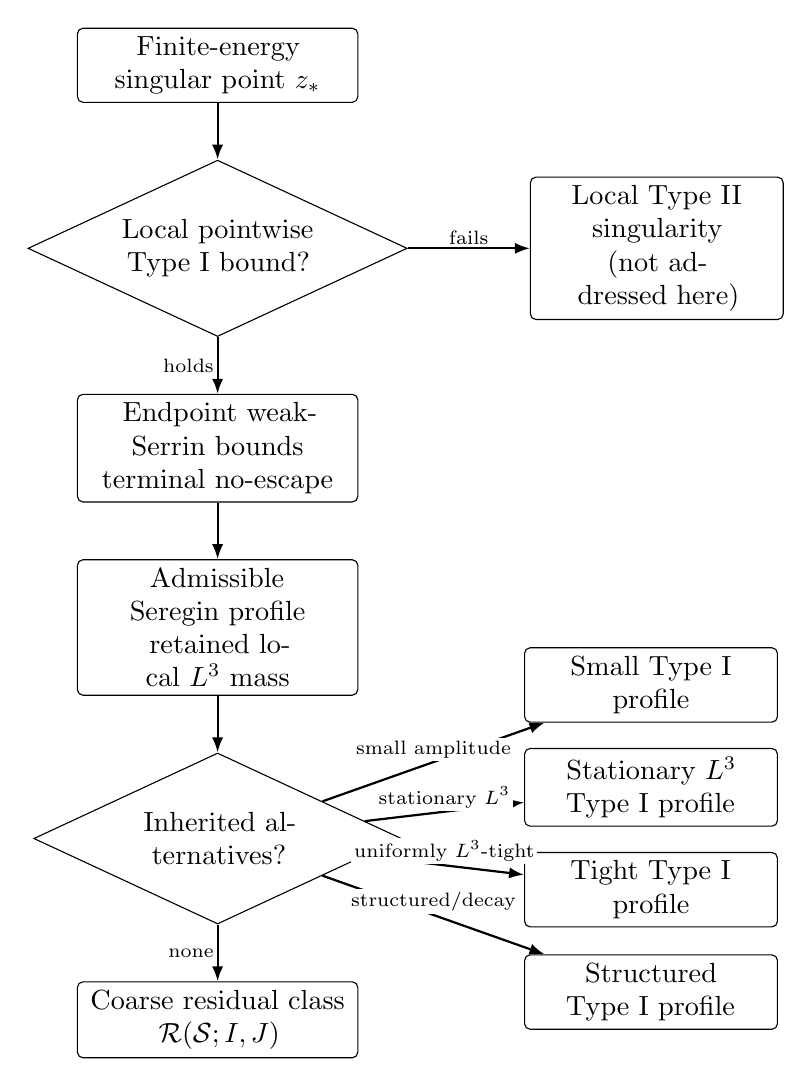
\begin{tikzpicture}[
   node distance=0.72cm and 1.20cm,
   process/.style={draw, rounded corners=2pt, align=center, text width=3.35cm,
      inner sep=3pt},
   decision/.style={draw, diamond, aspect=2.15, align=center, text width=2.95cm,
      inner sep=1.3pt},
   terminalnode/.style={draw, rounded corners=2pt, align=center, text width=3.00cm,
      inner sep=3pt},
   arrow/.style={-{Latex[length=1.9mm]}, thick},
   elab/.style={font=\scriptsize, inner sep=1pt, fill=white}
]
\node[process] (S) {Finite-energy singular point \(z_*\)};
\node[decision, below=of S] (QI) {Local pointwise Type~I bound?};
\node[terminalnode, right=1.55cm of QI] (TII)
   {Local Type~II singularity\\(not addressed here)};
\node[process, below=of QI] (WS)
   {Endpoint weak-Serrin bounds\\terminal no-escape};
\node[process, below=of WS] (SE)
   {Admissible Seregin profile\\retained local \(L^3\) mass};
\node[decision, below=of SE] (P13) {Inherited alternatives?};
\node[process, below=of P13] (R) {Coarse residual class\\\(\calR(\calS;I,J)\)};

\node[terminalnode, right=1.55cm of P13, yshift=1.95cm] (Lsmall)
   {Small Type~I profile};
\node[terminalnode, right=1.55cm of P13, yshift=0.65cm] (LstatL3)
   {Stationary \(L^3\)\\Type~I profile};
\node[terminalnode, right=1.55cm of P13, yshift=-0.65cm] (Ltight)
   {Tight Type~I profile};
\node[terminalnode, right=1.55cm of P13, yshift=-1.95cm] (Lstruct)
   {Structured Type~I profile};

\draw[arrow] (S) -- (QI);
\draw[arrow] (QI) -- node[elab, above] {fails} (TII);
\draw[arrow] (QI) -- node[elab, left] {holds} (WS);
\draw[arrow] (WS) -- (SE);
\draw[arrow] (SE) -- (P13);
\draw[arrow] (P13) -- node[elab, above] {small amplitude} (Lsmall);
\draw[arrow] (P13) -- node[elab, above] {stationary \(L^3\)} (LstatL3);
\draw[arrow] (P13) -- node[elab, above] {uniformly \(L^3\)-tight} (Ltight);
\draw[arrow] (P13) -- node[elab, above] {structured/decay} (Lstruct);
\draw[arrow] (P13) -- node[elab, left] {none} (R);
\end{tikzpicture}}
\caption{Rendered entry tree.  Local pointwise Type~I enters the
admissible Seregin framework through endpoint weak Serrin estimates and terminal
no-escape.  If the bound fails, the point belongs to the local Type~II
alternative, which is not addressed here.}
\label{fig:rendered-entry-tree}
\end{figure}

\begin{figure}[tbp]
\centering
\resizebox{0.98\textwidth}{!}{%
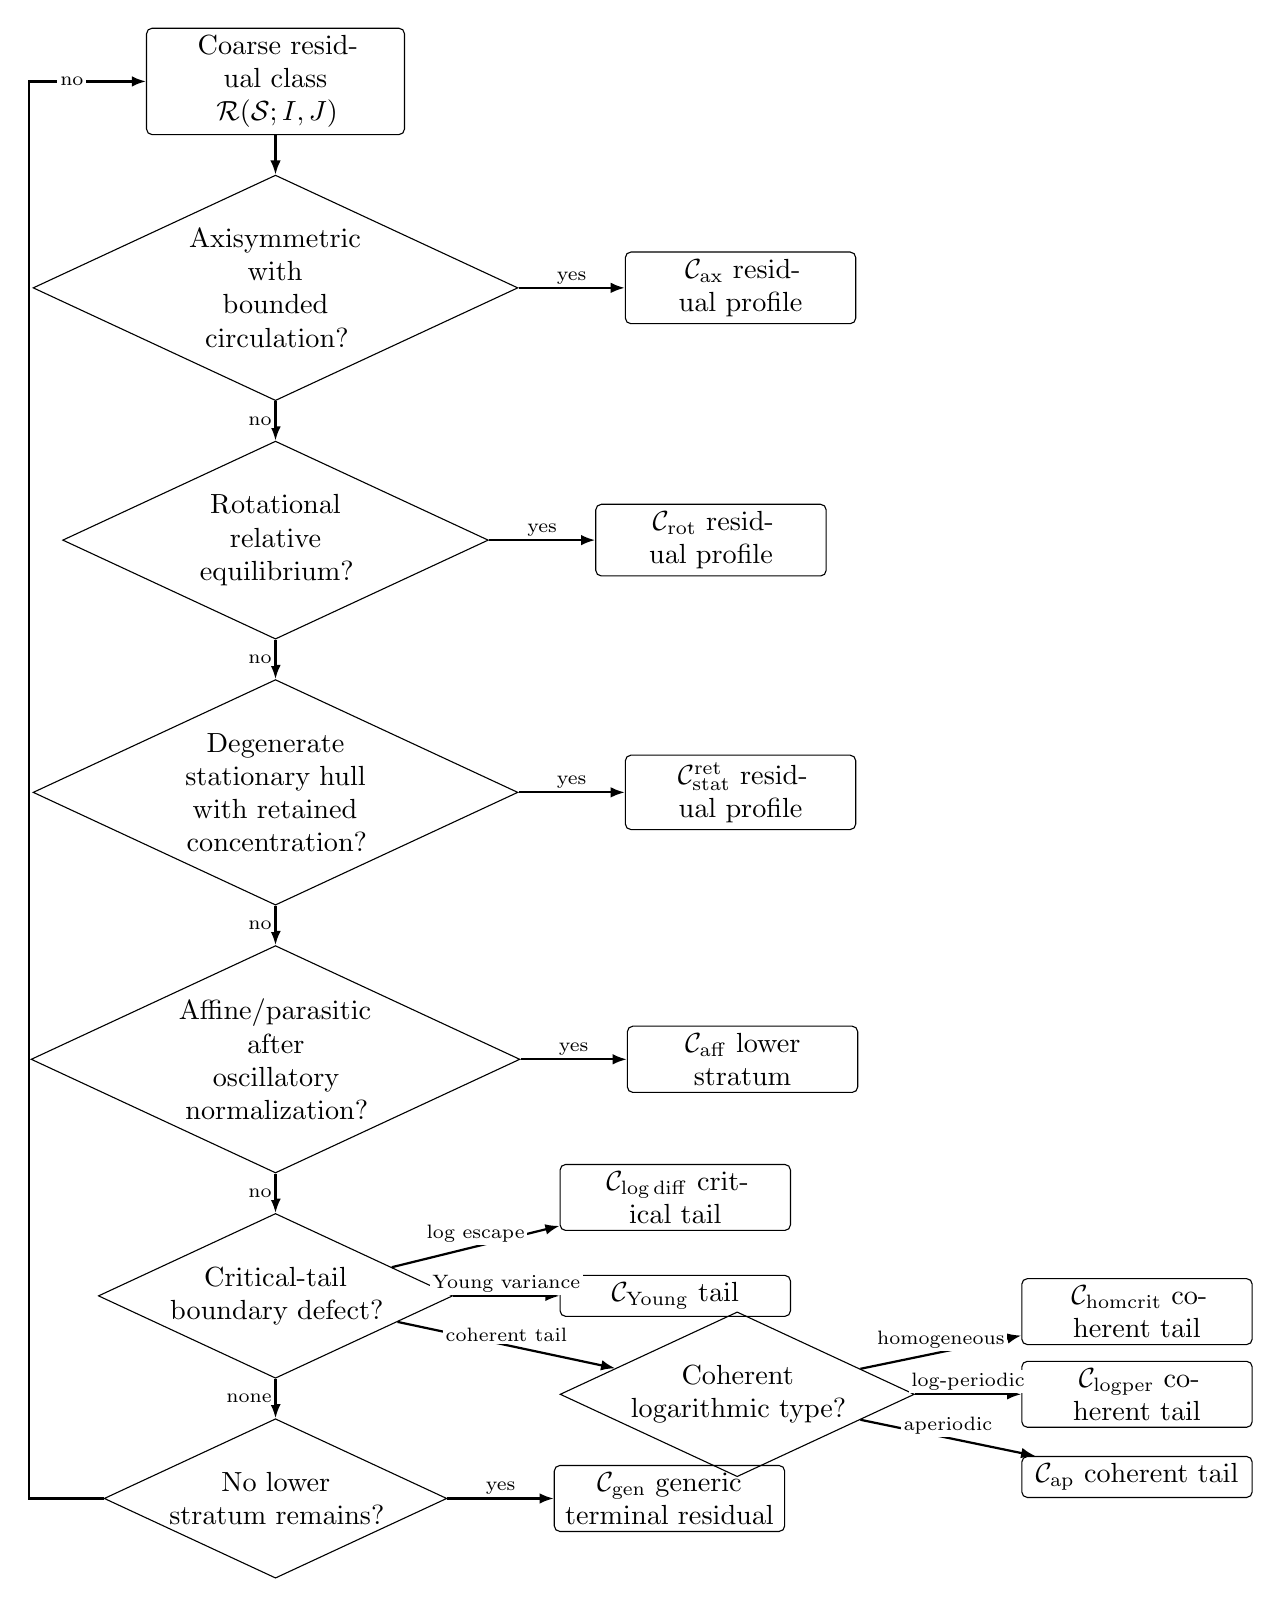
\begin{tikzpicture}[
   node distance=0.50cm and 1.08cm,
   process/.style={draw, rounded corners=2pt, align=center, text width=3.10cm,
      inner sep=2.5pt},
   decision/.style={draw, diamond, aspect=2.15, align=center, text width=2.70cm,
      inner sep=1pt},
   terminalnode/.style={draw, rounded corners=2pt, align=center, text width=2.75cm,
      inner sep=2.5pt},
   arrow/.style={-{Latex[length=1.8mm]}, thick},
   elab/.style={font=\scriptsize, inner sep=1pt, fill=white}
]
\node[process] (R) {Coarse residual class\\\(\calR(\calS;I,J)\)};
\node[decision, below=of R] (Qax) {Axisymmetric with\\bounded circulation?};
\node[terminalnode, right=1.35cm of Qax] (Lax) {\(\Cax\) residual profile};
\node[decision, below=of Qax] (Qrot) {Rotational relative\\equilibrium?};
\node[terminalnode, right=1.35cm of Qrot] (Lrot) {\(\Crot\) residual profile};
\node[decision, below=of Qrot] (Qst)
   {Degenerate stationary hull\\with retained concentration?};
\node[terminalnode, right=1.35cm of Qst] (Lst) {\(\Cstat\) residual profile};
\node[decision, below=of Qst] (Qaff)
   {Affine/parasitic after\\oscillatory normalization?};
\node[terminalnode, right=1.35cm of Qaff] (Laff) {\(\Caff\) lower stratum};
\node[decision, below=of Qaff] (Qtail) {Critical-tail\\boundary defect?};
\node[decision, below=of Qtail] (Qgen) {No lower stratum remains?};
\node[terminalnode, right=1.35cm of Qgen] (Lgen)
   {\(\Cgen\) generic terminal residual};

\node[terminalnode, right=1.35cm of Qtail, yshift=1.25cm] (Llog)
   {\(\Clogdiff\) critical tail};
\node[terminalnode, right=1.35cm of Qtail] (Lyng) {\(\Cyoung\) tail};
\node[decision, right=1.35cm of Qtail, yshift=-1.25cm] (Qcoh)
   {Coherent\\logarithmic type?};
\node[terminalnode, right=1.35cm of Qcoh, yshift=1.05cm] (Lhom)
   {\(\Chomcrit\) coherent tail};
\node[terminalnode, right=1.35cm of Qcoh] (Lper)
   {\(\Clogper\) coherent tail};
\node[terminalnode, right=1.35cm of Qcoh, yshift=-1.05cm] (Lap)
   {\(\Capcrit\) coherent tail};

\draw[arrow] (R) -- (Qax);
\draw[arrow] (Qax) -- node[elab, above] {yes} (Lax);
\draw[arrow] (Qax) -- node[elab, left] {no} (Qrot);
\draw[arrow] (Qrot) -- node[elab, above] {yes} (Lrot);
\draw[arrow] (Qrot) -- node[elab, left] {no} (Qst);
\draw[arrow] (Qst) -- node[elab, above] {yes} (Lst);
\draw[arrow] (Qst) -- node[elab, left] {no} (Qaff);
\draw[arrow] (Qaff) -- node[elab, above] {yes} (Laff);
\draw[arrow] (Qaff) -- node[elab, left] {no} (Qtail);
\draw[arrow] (Qtail) -- node[elab, above] {log escape} (Llog);
\draw[arrow] (Qtail) -- node[elab, above] {Young variance} (Lyng);
\draw[arrow] (Qtail) -- node[elab, above] {coherent tail} (Qcoh);
\draw[arrow] (Qcoh) -- node[elab, above] {homogeneous} (Lhom);
\draw[arrow] (Qcoh) -- node[elab, above] {log-periodic} (Lper);
\draw[arrow] (Qcoh) -- node[elab, above] {aperiodic} (Lap);
\draw[arrow] (Qtail) -- node[elab, left] {none} (Qgen);
\draw[arrow] (Qgen) -- node[elab, above] {yes} (Lgen);
\draw[arrow] (Qgen.west) -- ++(-0.95,0) |- node[elab, near end, left] {no}
   (R.west);
\end{tikzpicture}}
\caption{Rendered residual stratification tree.  The final return arrow only records
the ordered nature of the decomposition: if a lower stratum has not been
removed, the profile is assigned to that terminal alternative; after all lower
alternatives are removed,
the remaining residual class is \(\Cgen\).}
\label{fig:rendered-residual-tree}
\end{figure}

The loop from the last criterion back to the residual class is only a graphical
way to indicate the ordered nature of the decomposition: if a lower stratum has
not actually been removed, it is assigned to its corresponding terminal
alternative rather than
to \(\Cgen\).  After the ordered removals are performed, \(\Cgen\) is exactly
the remaining residual class by definition.
For the table, write
\[
   \mathfrak T_\rho(u;z_*):=
   \esssup_{T-\rho^2<t<T}
   \sqrt{T-t}\,\|u(t)\|_{L^\infty(B_\rho(x_*))}.
\]

\begingroup
\footnotesize
\setlength{\tabcolsep}{4pt}
\renewcommand{\arraystretch}{1.25}
\begin{longtable}{@{}L{1.20in}L{4.65in}@{}}
\caption{Classification and closure table for the decision tree.  Each row gives
the criterion selecting the terminal alternative, the mechanism that excludes
it when it is a Type~I alternative, and the statement used at that point.
For the inherited alternatives, the displayed condition is a representative
form of the inherited definition; the precise definitions and closures are those
of \(\texttt{proof\_setup.tex}\).}
\label{tab:decision-tree-classification}\\
\hline
\textbf{Terminal alternative} & \textbf{Criterion, exclusion mechanism, and reference}\\
\hline
\endfirsthead
\hline
\textbf{Terminal alternative} & \textbf{Criterion, exclusion mechanism, and reference}\\
\hline
\endhead
\hline
\endfoot
Local Type~II singularity &
\textbf{Criterion.}  For every \(\rho>0\),
\(\mathfrak T_\rho(u;z_*)=\infty\).
\textbf{Role.}  This is the complementary alternative left by the local
Type~I/Type~II dichotomy after local pointwise Type~I is excluded.
\textbf{Link.}  \Cref{cor:local-typeI-unconditional}.\\

Small Type~I profile &
\textbf{Criterion.}  Inherited small-amplitude class; schematically
\(\|V\|_{L^\infty(\R^3\times\R)}\le\eps_{\rm sm}\).
\textbf{Exclusion.}  Small-data/regularity closure recorded in the setup
paper.
\textbf{Link.}  \Cref{hyp:previous-nonresidual}.\\

Stationary \(L^3\) Type~I profile &
\textbf{Criterion.}  Inherited stationary class; representative condition
\(\partial_\tau V=0\) and \(V\in L^3(\R^3)\).
\textbf{Exclusion.}  Stationary \(L^3\) Liouville/regularity closure recorded
in the setup paper.
\textbf{Link.}  \Cref{hyp:previous-nonresidual}.\\

Tight Type~I profile &
\textbf{Criterion.}  Inherited tight class; representative condition
\(\lim_{R\to\infty}\sup_\tau\int_{|y|>R}|V(y,\tau)|^3\,dy=0\).
\textbf{Exclusion.}  Endpoint \(L^3\) rigidity for uniformly tight ancient
dynamics.
\textbf{Link.}  \Cref{hyp:previous-nonresidual}.\\

Structured Type~I profile &
\textbf{Criterion.}  Inherited closed structured/decay class,
\(V\in\mathcal C_{\rm struct/decay}^{\rm setup}\).
\textbf{Exclusion.}  Closed structured/decay alternatives recorded in the
setup paper.
\textbf{Link.}  \Cref{hyp:previous-nonresidual}.\\

\(\Cax\) residual profile &
\textbf{Criterion.}  Axisymmetric residual profile with bounded centered
circulation \(\Gamma(\rho,Z,\tau)=\rho V_\theta\) and
\(\|\Gamma\|_{L^\infty}<\infty\).
\textbf{Exclusion.}  Centered circulation equation plus axis-absorption
Liouville theorem; the profile becomes no-swirl and falls into an earlier
structured class.
\textbf{Link.}  \Cref{thm:R1-exclusion}.\\

\(\Crot\) residual profile &
\textbf{Criterion.}  Rotational relative equilibrium
\(V(y,\tau)=Q(\tau)W(Q(\tau)^Ty)\), \(Q(\tau)=e^{\tau\Omega}\).
\textbf{Exclusion.}  Localized Coriolis-flux reduction into the terminal local
concentration decomposition.
\textbf{Link.}  \Cref{thm:R2-exclusion-safe}.\\

\(\Cstat\) residual profile &
\textbf{Criterion.}  Degenerate stationary-hull retained profile: along
time translations \(T_{s_k}V\to W\), where \(W\) is stationary and
\(\calE_1(W,\Pi;0)\ge\eps_*\).
\textbf{Exclusion.}  Scale reselection reduces to a stationary retained
concentration profile, then terminal concentration excludes it.
\textbf{Link.}  \Cref{thm:R3S-R3-empty}.\\

\(\Caff\) lower stratum &
\textbf{Criterion.}  Affine-normalized oscillatory activity vanishes:
\(\Phi(S_cU)=0\) for an admissible affine symmetry \(S_c\).
\textbf{Exclusion.}  Oscillatory entry normalization forces retained residual
states to keep positive non-affine activity after affine normalization.
\textbf{Link.}  \Cref{thm:oscillatory-entry-normalization}.\\

\(\Clogdiff\) critical tail &
\textbf{Criterion.}  Logarithmic escape component in the realized
critical-tail compactification: \(\Lambda\ne0\).
\textbf{Exclusion.}  Log-window descendant selection plus minimal
mesoscopic-scale reduction and hidden-scale compactness.
\textbf{Link.}  \Cref{cor:log-diffuse-branch-discharge}.\\

\(\Cyoung\) tail &
\textbf{Criterion.}  Tight annular critical-tail state with non-Dirac Young
measure: \(\Lambda=0\) and
\(\mathcal Y_{x,s}\ne\delta_{\bar W(x,s)}\) on a set of positive measure.
\textbf{Exclusion.}  No hidden-scale variance gives strong
\(L^3_{\loc}\) compactness, hence a Dirac Young measure.
\textbf{Link.}  \Cref{cor:young-branch-discharge}.\\

\(\Chomcrit\) coherent tail &
\textbf{Criterion.}  Coherent \((-1)\)-homogeneous tail:
\(W(r\omega,s)=r^{-1}A(\omega,s)\).
\textbf{Exclusion.}  Bounded-origin realization gives
\(W\in L^\infty_{\loc}\) near \(r=0\), forcing \(A=0\).
\textbf{Link.}  \Cref{cor:coherent-critical-tail-branch-closure}.\\

\(\Clogper\) coherent tail &
\textbf{Criterion.}  Nonzero log-periodic coherent tail:
\(Z(\rho+L,\omega,s)=Z(\rho,\omega,s)\), \(L\ne0\), where
\(Z=e^\rho W(e^\rho\omega,s)\).
\textbf{Exclusion.}  Bounded-origin realization gives
\(Z(\rho,\cdot,\cdot)\to0\) as \(\rho\to-\infty\); periodicity forces
\(Z\equiv0\).
\textbf{Link.}  \Cref{cor:coherent-critical-tail-branch-closure}.\\

\(\Capcrit\) coherent tail &
\textbf{Criterion.}  Nonzero aperiodic minimal logarithmic hull:
\(\mathcal H(Z)\) is minimal, nonperiodic, and nonzero.
\textbf{Exclusion.}  Bounded-origin realization puts \(0\) in the compact
log-translation hull; minimality forces the hull to be \(\{0\}\).
\textbf{Link.}  \Cref{cor:coherent-critical-tail-branch-closure}.\\

\(\Cgen\) generic terminal residual &
\textbf{Criterion.}  Ordered complement
\[
   V\in\calR(\calS;I,J)
   \setminus\bigcup_{\mathcal B\in\mathfrak B_{\rm lower}}\mathcal B ,
\]
where \(\mathfrak B_{\rm lower}\) is the list of all preceding Type~I
alternatives.
\textbf{Exclusion.}  Paired active-locus decomposition, finite
separated-family exclusion, terminal indecomposability, sequence-\(L^3\),
parasitic-free mildness, and the Albritton--Barker endpoint Liouville theorem.
\textbf{Link.}  \Cref{thm:R4-final-closure}.\\
\end{longtable}
\endgroup

\section{Shared local notation}
\label{sec:shared-notation}

For \(z_0=(y_0,\tau_0)\) and \(r>0\), write
\[
   Q_r(z_0):=B_r(y_0)\times(\tau_0-r^2,\tau_0).
\]
For a centered profile \((V,P)\), the pressure-normalized local critical
quantity is
\begin{equation}\label{eq:local-energy-main}
   \calE_r(V,P;z_0)
   :=
   \iint_{Q_r(z_0)}
   \left(|V|^3+|P-c_{r,z_0}(\tau)|^{3/2}\right)\,dy\,d\tau,
\end{equation}
where \(c_{r,z_0}(\tau)\) is an allowed time-dependent pressure gauge, usually
chosen as a spatial average over \(B_r(y_0)\).  All local pressure
convergences below are understood after such gauges.

\begin{definition}[Retained local concentration profile]
\label{def:retained-active-main}
Fix \(\eps_*>0\).  A terminal profile \((U,\Pi)\) has retained local
concentration if, after the terminal normalization under consideration,
\[
   \calE_1(U,\Pi;0)\ge \eps_* .
\]
\end{definition}

\begin{definition}[Threshold hierarchy]
\label{def:threshold-hierarchy}
The constants used in the terminal concentration argument are chosen in the following order.
The compact velocity lower bounds \(\eta_0\) and \(\eta_v\) are supplied by
the setup paper \(\texttt{proof\_setup.tex}\) and the local concentration input
therein, respectively.  The local small-data threshold
\(\eps_{\rm sd}\) is then fixed with
\[
   0<\eps_{\rm sd}\le \min\{\eta_0,\eta_v,\eps_{\CKN}\},
\]
where \(\eps_{\CKN}\) denotes the universal CKN regularity threshold whenever
that threshold is invoked.  The retained descendant threshold \(\eps_*\) is
chosen after the pressure gauges and compactness topology are fixed, with
\[
   0<\eps_*\le \frac12\eps_{\rm sd}.
\]
Whenever a compactness or lower-semicontinuity passage loses a harmless fixed
factor, \(\eps_*\) is replaced once and for all by a smaller positive value.
No later argument chooses a new concentration threshold depending on a
previously extracted profile tree.
\end{definition}

\begin{definition}[Refined residual candidate]
\label{def:refined-residual-candidate}
A refined residual candidate is a bounded normalized Seregin ancient limit
obtained from the admissible Seregin extraction theorem in
\(\texttt{proof\_setup.tex}\), which carries the positive compact local velocity
mass in \eqref{eq:positive-velocity-main}, and which is not in any alternative
already closed before the refined residual decomposition is entered.  The
definition is local: the only persistent lower bound attached to the candidate by
the setup paper is the fixed compact velocity \(L^3\) lower bound.
\end{definition}

\begin{remark}[No hidden global \(L^3\) assertion]
\label{rem:no-hidden-global-L3}
The terminal arguments below do not claim that a generic residual profile is
globally \(L^3\)-tight or globally bounded in \(L^\infty_\tau L^3_y\).  The
only nonlocal critical-norm conclusion used at the endpoint is the weaker
sequence-\(L^3\) completeness of retained indecomposable concentration
profiles, and that conclusion is derived from local terminal alternatives rather than from an
a priori global estimate on the original residual class.
\end{remark}

\subsection{Notation, threshold, and gauge directories}
\label{subsec:notation-directories}

The following compact directories collect the persistent symbols, thresholds,
and gauges used in the residual closure.  They are not new definitions; each
entry refers to the location where the object is first defined.

\paragraph{Velocity, pressure, and state-space symbols.}
\begin{itemize}[leftmargin=1.6em]
   \item \((V,P)\): centered Seregin ancient profile in \eqref{eq:centered-main};
      first used in \Cref{sec:introduction}.
   \item \((U,Q)\): physical ancient representative when \((V,P)\) is treated
      under physical pullback \eqref{eq:physical-pullback-main}; also used in
      \(\calR_z\)-recentered form throughout
      \Cref{sec:R4-tail-geometry,sec:terminal-concentration}.  The intended
      meaning is fixed locally in each section by the explicit definition of
      the immediately preceding rescaling.
   \item \((W,Q_W)\): blown-down, co-rotating, or tail profile, depending on
      the section; defined locally in
      \Cref{sec:R2-reduction,subsec:hidden-scale-young-variance}.
   \item \(\calE_r(V,P;z_0)\): pressure-normalized local critical quantity, see
      \eqref{eq:local-energy-main}.
   \item \(\calE_1\): pressure-normalized unit CKN activity, fixed at
      \(r=1\); used throughout the terminal concentration arguments and in the
      retained-concentration definition \Cref{def:retained-active-main}.
   \item \(\Tcrit\): terminal state space, \Cref{def:terminal-state-space}.
   \item \(\Tcrit^\#\): compact normalized descendant state space,
      \Cref{def:compact-normalized-state-space}.
   \item \(\Caff\): affine/parasitic routing/quotient stratum,
      \Cref{def:affine-constant-lower-stratum}; not a usual nonempty/empty PDE
      class but a discharge label, see
      \Cref{rem:affine-constant-use,thm:oscillatory-entry-normalization}.
   \item \(\oscsp\): spatial oscillation modulo time-dependent homogeneous
      gauges, \Cref{def:multiscale-affine-oscillation}.
   \item \(\actthree\) and \(\Phi\): constant-mode/non-affine retained
      activity, \Cref{def:observer-oscillation,thm:closed-nonaffine-activity}.
\end{itemize}

\paragraph{Threshold ordering.}
\begin{itemize}[leftmargin=1.6em]
   \item \(\eta_0\): compact velocity \(L^3\) lower bound supplied by the base
      Seregin extraction \Cref{hyp:base-seregin-package}.
   \item \(\eta_v\): compact velocity lower bound from the local concentration
      input of the setup paper, used as initial mass for terminal extraction;
      see \Cref{def:threshold-hierarchy}.
   \item \(\eps_{\rm sd}\): local small-data threshold,
      \(0<\eps_{\rm sd}\le\min\{\eta_0,\eta_v,\eps_{\CKN}\}\),
      \Cref{def:threshold-hierarchy}.
   \item \(\eps_*\): retained descendant CKN threshold,
      \(0<\eps_*\le\eps_{\rm sd}/2\), used in
      \Cref{def:retained-active-main} and in active-locus extraction.
   \item \(\eps_0\): minimal mesoscopic-scale oscillation threshold; depends
      only on the hidden-scale defect lower bound and on the finite-overlap
      constants of \Cref{lem:finite-overlap-affine-oscillation}; first appears
      in \Cref{def:first-bad-mesoscopic-scale}.
   \item \(\eta_K\): compact-activity lower bound on the recurrent active core,
      first introduced in \Cref{thm:active-path-space-recurrence}.
\end{itemize}
The thresholds are fixed in the order
\(\eta_0,\eta_v\Rightarrow\eps_{\rm sd}\Rightarrow\eps_*\Rightarrow\eps_0,
\eta_K\), and no later argument chooses a new concentration threshold depending
on a previously extracted profile tree.  Phrases of the form ``after lowering
the threshold'' refer either to the once-and-for-all reduction of \(\eps_*\)
recorded in \Cref{def:threshold-hierarchy} or to a slight reduction of the
mesoscopic threshold \(\eps_0\) recorded in
\Cref{lem:h2-failure-first-bad-scale}; in either case the reduction does not
disturb earlier choices.

\paragraph{Pressure and velocity gauges.}
\begin{itemize}[leftmargin=1.6em]
   \item \(c_{r,z_0}(\tau)\): local pressure time gauge in
      \eqref{eq:local-energy-main}; measurable in \(\tau\); used because
      pressure is defined modulo functions of time.
   \item \(c_n(s)\): homogeneous velocity gauge at the minimal mesoscopic
      scale, \Cref{def:first-bad-spatial-blowdown}; bounded; either compactifies
      or routes the descendant to \(\Caff\) by
      \Cref{lem:homogeneous-gauge-compactness}; no pointwise derivative
      \(\partial_s c_n\) is used unless that compactness has already been
      obtained.
   \item \(\beta(s)\cdot y+\alpha(s)\): affine parasitic pressure paired with a
      spatially homogeneous velocity mode; quotient notation introduced in
      \Cref{def:affine-constant-lower-stratum} and used only in the gauged
      formulation of the affine/parasitic stratum.
   \item \(L_n(x,s)=b_n(s)\cdot x+a_n(s)\): scaled affine pressure at the
      minimal mesoscopic scale, \Cref{lem:scaled-pressure-compactness-affine};
      affine in \(x\), measurable in \(s\); discarded in the non-affine quotient
      and routed to \(\Caff\) when it does not vanish.
   \item \(a_{n,K}(t)\): local Seregin pressure time gauge on a compact
      cylinder \(K\), used by the local pressure-gauge compactness package
      inherited from the setup paper and recorded in
      \Cref{prop:local-typeI-terminal-compactness}.
\end{itemize}

\section{Exclusion of the axisymmetric bounded-circulation residual class}
\label{sec:R1-exclusion}

In this section we prove the rigidity statement needed for the first refined
residual class.  The argument uses the scale-invariant angular circulation in
centered variables.  The essential point is that the centered Type~I equation
contains the Ornstein--Uhlenbeck drift.  Thus the angular-circulation equation
has an absorbing boundary at the symmetry axis together with a confining drift
at spatial infinity.  This gives a scalar Liouville theorem for bounded ancient
solutions of the circulation equation.  Related axisymmetric Liouville theorems
for Navier--Stokes, in different settings, are proved in
\cite{LZZ2017,LRZ2022}.

Throughout the section we write cylindrical coordinates as
\((\rho,\theta,Z)\), and an axisymmetric vector field as
\[
   V=V_\rho e_\rho+V_\theta e_\theta+V_Z e_Z .
\]
The centered Navier--Stokes equation is
\begin{equation}\label{eq:centered-R1}
   \partial_\tau V-\Delta V+\frac12 y\cdot\nabla V+\frac12 V
   +(V\cdot\nabla)V+\nabla P=0,
   \qquad \nabla\cdot V=0 .
\end{equation}
For an axisymmetric solution define the centered angular circulation
\begin{equation}\label{eq:centered-Gamma-def}
   \Gamma(\rho,Z,\tau):=\rho V_\theta(\rho,Z,\tau).
\end{equation}
This is the same scale-invariant quantity as the physical circulation
\(rU_\theta\).  If the physical representative is
\[
   U(x,t)=(-t)^{-1/2}V(x/\sqrt{-t},-\log(-t)),
\]
then
\[
   rU_\theta(r,z,t)=\rho V_\theta(\rho,Z,\tau),
   \qquad r=\sqrt{-t}\,\rho,
   \quad z=\sqrt{-t}\,Z.
\]

\begin{lemma}[Centered circulation equation]\label{lem:centered-circulation-equation}
Let \((V,P)\) be a smooth bounded axisymmetric solution of
\eqref{eq:centered-R1}.  Then \(\Gamma=\rho V_\theta\) satisfies
\begin{equation}\label{eq:centered-Gamma-equation}
   \partial_\tau\Gamma
   =
   \partial_\rho^2\Gamma-\frac1\rho\partial_\rho\Gamma
      +\partial_Z^2\Gamma
   -\left(V_\rho+\frac\rho2\right)\partial_\rho\Gamma
   -\left(V_Z+\frac Z2\right)\partial_Z\Gamma
\end{equation}
on \((0,\infty)\times\mathbb R\times\mathbb R\).  Moreover
\begin{equation}\label{eq:axis-boundary-Gamma}
   \Gamma(0,Z,\tau)=0
   \qquad\hbox{for all }(Z,\tau)\in\mathbb R\times\mathbb R .
\end{equation}
\end{lemma}

\begin{proof}
The angular component of \eqref{eq:centered-R1} is
\[
   \partial_\tau V_\theta
   -\left(\Delta-\frac1{\rho^2}\right)V_\theta
   +\frac12(\rho\partial_\rho+Z\partial_Z)V_\theta
   +\frac12V_\theta
   +V_\rho\partial_\rho V_\theta+V_Z\partial_ZV_\theta
   +\frac{V_\rho V_\theta}{\rho}=0 .
\]
Multiplying by \(\rho\), using
\[
   \rho\left(\Delta-\frac1{\rho^2}\right)V_\theta
   =\partial_\rho^2\Gamma-\frac1\rho\partial_\rho\Gamma+
      \partial_Z^2\Gamma,
\]
\[
   \rho\left[\frac12(\rho\partial_\rho+Z\partial_Z)V_\theta
      +\frac12V_\theta\right]
   =\frac12(\rho\partial_\rho+Z\partial_Z)\Gamma,
\]
and
\[
   \rho\left(V_\rho\partial_\rho V_\theta+V_Z\partial_ZV_\theta
      +\frac{V_\rho V_\theta}{\rho}\right)
   =V_\rho\partial_\rho\Gamma+V_Z\partial_Z\Gamma,
\]
gives \eqref{eq:centered-Gamma-equation}.  Finally, smoothness of a bounded
axisymmetric vector field at the axis implies \(V_\theta(\rho,Z,\tau)=O(\rho)\)
as \(\rho\downarrow0\), locally uniformly in \((Z,\tau)\).  Hence
\(\Gamma=\rho V_\theta=O(\rho^2)\), which gives
\eqref{eq:axis-boundary-Gamma}.
\end{proof}

We next record the scalar Liouville theorem used below.  It is stated in a
form that isolates precisely the PDE mechanism: bounded drift perturbations of
the centered circulation operator cannot sustain a bounded ancient solution
which vanishes on the symmetry axis.

\begin{lemma}[Axis-absorption Liouville theorem]
\label{lem:axis-absorption-liouville}
Let \(B=(B_\rho,B_Z)\) be a smooth vector field on
\((0,\infty)\times\mathbb R\times\mathbb R\) satisfying
\[
   \|B\|_{L^\infty}<\infty .
\]
Let \(G\in C^{2,1}((0,\infty)\times\mathbb R\times\mathbb R)\cap L^\infty\)
solve
\begin{equation}\label{eq:abstract-Gamma-equation}
   \partial_\tau G
   =
   \partial_\rho^2G-\frac1\rho\partial_\rho G+
      \partial_Z^2G
   -\left(B_\rho+\frac\rho2\right)\partial_\rho G
   -\left(B_Z+\frac Z2\right)\partial_ZG
\end{equation}
for all \(\tau\in\mathbb R\), and assume
\begin{equation}\label{eq:abstract-axis-zero}
   \lim_{\rho\downarrow0}G(\rho,Z,\tau)=0
   \qquad\hbox{locally uniformly in }(Z,\tau).
\end{equation}
Then \(G\equiv0\).
\end{lemma}

\begin{proof}
Set \(M_B=\|B\|_{L^\infty}\).  For \(R>1\) define
\begin{equation}\label{eq:radial-barrier}
   h_R(\rho)
   :=
   \frac{\displaystyle\int_0^{\min\{\rho,R\}} s
      \exp\left(\frac{s^2}{4}-M_Bs\right)\,ds}
   {\displaystyle\int_0^R s
      \exp\left(\frac{s^2}{4}-M_Bs\right)\,ds} .
\end{equation}
Then \(0\le h_R\le1\), \(h_R(0)=0\), \(h_R(R)=1\), and, on
\(0<\rho<R\),
\begin{equation}\label{eq:hR-ode}
   h_R''+\left(M_B-\frac\rho2-\frac1\rho\right)h_R'=0,
   \qquad h_R'>0 .
\end{equation}
Let
\[
   \mathcal L_\tau f
   :=
   \partial_\rho^2f-\frac1\rho\partial_\rho f+\partial_Z^2f
   -\left(B_\rho+\frac\rho2\right)\partial_\rho f
   -\left(B_Z+\frac Z2\right)\partial_Z f .
\]
Since \(B_\rho\ge -M_B\), \eqref{eq:hR-ode} gives
\begin{equation}\label{eq:hR-superharmonic}
   \mathcal L_\tau h_R
   =h_R''-\left(\frac1\rho+\frac\rho2+B_\rho\right)h_R'
   \le
   h_R''+\left(M_B-\frac\rho2-\frac1\rho\right)h_R'
   =0 .
\end{equation}
Thus \((\partial_\tau-\mathcal L_\tau)h_R\ge0\).

We now compare \(G\) to this barrier on the strip
\(\Omega_R=(0,R)\times\mathbb R\).  Let
\(M_G=\|G\|_{L^\infty}\).  We first record the Dirichlet strip decay estimate used
by the comparison argument.  If \(q_{s,R}\) solves
\[
   \partial_\tau q_{s,R}=\mathcal L_\tau q_{s,R},
   \qquad q_{s,R}=0\hbox{ on }\rho=0,R,
   \qquad q_{s,R}(\rho,Z,s)=1,
\]
then, for every compact \(K\Subset\Omega_R\) and every fixed \(t\),
\begin{equation}\label{eq:killed-strip-decay}
   \lim_{s\to-\infty}\sup_{(\rho,Z)\in K}q_{s,R}(\rho,Z,t)=0 .
\end{equation}
To prove \eqref{eq:killed-strip-decay}, fix \(K\Subset\Omega_R\).  Choose
\(\delta>0\), \(Z_K>0\), and \(Z_1>Z_K+1\) so that
\[
   K\subset [\delta,R-\delta]\times[-Z_K,Z_K]
   \subset (0,R)\times(-Z_1,Z_1).
\]
On the finite cylinder
\[
   \Omega_{R,Z_1}:=(0,R)\times(-Z_1,Z_1)
\]
with Dirichlet data on the full parabolic boundary, the operator
\(\mathcal L_\tau\) is uniformly parabolic on
\([\delta/2,R-\delta/2]\times[-Z_1,Z_1]\), has bounded first-order coefficients
there, and has absorbing boundary at \(\rho=0,R\).  The boundary parabolic
Harnack inequality and the strong maximum principle give a time \(T_R>0\) and a
number \(\vartheta_R\in(0,1)\), depending only on
\(R,M_B,\delta,Z_K\) and not on \(Z_1\), such that every nonnegative solution
with initial data bounded by \(1\) and zero lateral data satisfies
\[
   0\le q(\cdot,s+T_R)\le 1-\vartheta_R
   \qquad\hbox{on }[\delta,R-\delta]\times[-Z_K,Z_K].
\]
Applying the same estimate after each time translation and using the maximum
principle between the compact set and the boundary gives
\[
   \sup_K q_{s,R}(\cdot,s+mT_R)
   \le (1-\vartheta_R)^m,\qquad m=1,2,\dots .
\]
For a fixed \(t>s\), choose \(m\) with
\(s+mT_R\le t<s+(m+1)T_R\).  The maximum principle and interior Harnack estimate
on the final interval \([s+mT_R,t]\) preserve the preceding bound up to a
constant depending only on \(R,M_B,\delta,Z_K,T_R\).  Letting \(s\to-\infty\)
forces \(m\to\infty\), proving decay on \(K\) for the truncated problem.  The
solutions on \(\Omega_{R,Z_1}\) increase monotonically to the Dirichlet strip
solution as \(Z_1\to\infty\); passing to this limit gives
\eqref{eq:killed-strip-decay}.

Fix \(R>1\), \(s<t\), and set
\[
   W^+_{R}:=\frac{G}{M_G}-h_R,
   \qquad
   W^-_{R}:=-\frac{G}{M_G}-h_R,
\]
with the convention that the conclusion is immediate if \(M_G=0\).
By \eqref{eq:abstract-Gamma-equation} and \eqref{eq:hR-superharmonic},
\[
   (\partial_\tau-\mathcal L_\tau)W_R^\pm\le0
   \qquad\hbox{in }\Omega_R\times(s,t).
\]
On \(\rho=0\), \eqref{eq:abstract-axis-zero} and \(h_R(0)=0\) give
\(W_R^\pm\le0\).  On \(\rho=R\), \(h_R(R)=1\) and \(|G|\le M_G\) give again
\(W_R^\pm\le0\).  The parabolic comparison principle with the Dirichlet strip
kernel therefore yields, for \(\tau=t\),
\[
   (W_R^\pm)_+(\rho,Z,t)
   \le q_{s,R}(\rho,Z,t)
   \qquad ((\rho,Z)\in\Omega_R).
\]
Letting \(s\to-\infty\) and using \eqref{eq:killed-strip-decay} gives
\(W_R^\pm\le0\) on compact subsets of \(\Omega_R\).  Since the compact subset
is arbitrary,
\begin{equation}\label{eq:G-bounded-by-hR}
   |G(\rho,Z,t)|\le M_G h_R(\rho)
   \qquad (0<\rho<R, Z\in\mathbb R,
   \ t\in\mathbb R).
\end{equation}
Finally, for each fixed \(\rho<\infty\), the denominator in
\eqref{eq:radial-barrier} tends to infinity super-exponentially as
\(R\to\infty\), while the numerator remains fixed.  Hence
\(h_R(\rho)\to0\).  Letting \(R\to\infty\) in
\eqref{eq:G-bounded-by-hR} gives \(G(\rho,Z,t)=0\) for every
\(\rho>0\), \(Z\in\mathbb R\), and \(t\in\mathbb R\).  The boundary value at
\(\rho=0\) is already zero by assumption.  Therefore \(G\equiv0\).
\end{proof}

\begin{theorem}[Exclusion of the axisymmetric bounded-circulation residual class]
\label{thm:R1-exclusion}
Let \(\Cax(\mathcal S;I,J)\) be the axisymmetric bounded-circulation residual
class in the refined residual decomposition.  Then
\begin{equation}\label{eq:R1-empty}
   \Cax(\mathcal S;I,J)=\varnothing .
\end{equation}
\end{theorem}

\begin{proof}
Assume, for contradiction, that
\(V\in\Cax(\mathcal S;I,J)\).  By definition of \(\Cax\), the
associated physical ancient representative is axisymmetric and has bounded
angular circulation.  Equivalently, in centered variables,
\[
   \Gamma(\rho,Z,\tau)=\rho V_\theta(\rho,Z,\tau)
\]
is bounded on \((0,\infty)\times\mathbb R\times\mathbb R\).  Since \(V\) is a
Seregin ancient limit, it is smooth and bounded in centered variables.  Hence
\(B=(V_\rho,V_Z)\) is bounded.

By \Cref{lem:centered-circulation-equation}, \(\Gamma\) satisfies
\eqref{eq:centered-Gamma-equation} and vanishes at the axis.  Applying
\Cref{lem:axis-absorption-liouville} with \(G=\Gamma\) and
\(B=(V_\rho,V_Z)\) gives
\[
   \Gamma\equiv0 .
\]
Therefore \(V_\theta\equiv0\) for \(\rho>0\), and by smoothness also on the
axis.  Thus the associated ancient solution is axisymmetric without swirl.
But the axisymmetric no-swirl class is one of the structured alternatives
removed before the residual class is defined.  This contradicts
\(V\in\mathcal R(\mathcal S;I,J)\), and therefore no such \(V\) exists.
\end{proof}

\begin{remark}[Why this does not assert the full bounded-swirl Liouville theorem]
The proof uses the centered Type~I equation, specifically the
Ornstein--Uhlenbeck drift terms \(-\rho\partial_\rho/2\) and
\(-Z\partial_Z/2\) in the scalar equation for \(\Gamma\).  It is therefore a
Type~I Seregin limit argument.  It does not prove that every bounded ancient
axisymmetric solution of the unrenormalized Navier--Stokes equations with
bounded physical circulation is swirl-free.  The latter lacks the confining
centered drift and remains a different shell-transport problem.
\end{remark}


\section{The rotational relative-equilibrium residual class}
\label{sec:R2-reduction}

We next isolate the second refined residual class.  This class consists of
centered Type~I ancient limits whose time dependence is a rigid rotation of a
fixed spatial profile.  Passing to the co-rotating frame converts the centered
Navier--Stokes equation into a stationary Leray profile equation with a
Coriolis transport term.  A whole-space Coriolis--Leray Liouville theorem for
all bounded profiles is not used here.  Instead, the Coriolis term is localized as an annular
flux and is then treated by the local concentration analysis proved in
\Cref{sec:terminal-concentration,sec:separated-profiles-atomic}.

Throughout this section the centered equation is
\begin{equation}\label{eq:centered-R2-safe}
   \partial_\tau V-\Delta V+\frac12 y\cdot\nabla V+\frac12 V
   +(V\cdot\nabla)V+\nabla P=0,
   \qquad \nabla\cdot V=0 .
\end{equation}
For \(\Omega\in\mathfrak{so}(3)\), set
\begin{equation}\label{eq:rotation-group-R2-safe}
   Q(\tau):=\exp(\tau\Omega)\in SO(3).
\end{equation}

\begin{definition}[Rotational relative-equilibrium profile]
\label{def:R2-relative-profile-safe}
A bounded smooth ancient solution \((V,P)\) of \eqref{eq:centered-R2-safe} is a
rotational relative equilibrium if there exist
\(\Omega\in\mathfrak{so}(3)\), a bounded smooth divergence-free vector field
\(W\), and a pressure profile \(\Pi\), such that
\begin{equation}\label{eq:R2-relative-form-safe}
   V(y,\tau)=Q(\tau)W(Q(\tau)^Ty),
   \qquad
   P(y,\tau)=\Pi(Q(\tau)^Ty)
\end{equation}
up to the usual time-dependent pressure gauge.
The class \(\Crot\) consists of such residual Seregin profiles, after the
axisymmetric bounded-circulation class and the previously closed alternatives in
the setup paper have been removed.
\end{definition}

\begin{lemma}[Co-rotating stationary equation]
\label{lem:co-rotating-equation-safe}
Let \((V,P)\) be a rotational relative equilibrium.  Then the co-rotating
profile \((W,\Pi)\) satisfies
\begin{equation}\label{eq:R2-coriolis-profile-safe}
   -\Delta W+\frac12 y\cdot\nabla W+\frac12 W
   +(W\cdot\nabla)W
   +\Omega W-(\Omega y)\cdot\nabla W
   +\nabla\Pi=0,
   \qquad \nabla\cdot W=0 .
\end{equation}
Equivalently,
\begin{equation}\label{eq:R2-coriolis-profile-project-safe}
   \mathbb P\Big[
   -\Delta W+\frac12 y\cdot\nabla W+\frac12 W
   +(W\cdot\nabla)W
   +\Omega W-(\Omega y)\cdot\nabla W
   \Big]=0,
\end{equation}
where \(\mathbb P\) is the whole-space Leray projector.
\end{lemma}

\begin{proof}
Let \(z=Q(\tau)^Ty\).  Since \(Q'(\tau)=\Omega Q(\tau)\) and
\(Q(\tau)^T\Omega Q(\tau)=\Omega\), one has
\[
   \partial_\tau z=-\Omega z.
\]
Therefore
\[
   \partial_\tau V(y,\tau)
   =Q(\tau)\Big(\Omega W(z)-(\Omega z)\cdot\nabla W(z)\Big).
\]
The Laplacian, divergence, convection term, and pressure gradient are invariant
under the orthogonal change of variables.  Substitution into
\eqref{eq:centered-R2-safe}, followed by multiplication by \(Q(\tau)^T\), gives
\eqref{eq:R2-coriolis-profile-safe}.  Applying the Leray projector gives
\eqref{eq:R2-coriolis-profile-project-safe}.
\end{proof}

\subsection{The Bernoulli identity and the local Coriolis flux}

Write
\begin{equation}\label{eq:R2-F-def}
   F(y):=\frac12y-\Omega y,
   \qquad
   A(y):=W(y)+F(y),
   \qquad
   \omega:=\nabla\times W .
\end{equation}
Since \(\Omega\) is skew-symmetric, there is a unique vector
\(\varpi\in\mathbb R^3\) such that
\begin{equation}\label{eq:R2-Omega-vector}
   \Omega y=\varpi\times y .
\end{equation}
Then
\begin{equation}\label{eq:R2-curlF}
   \nabla\times F=-2\varpi .
\end{equation}

\begin{lemma}[Coriolis Bernoulli identity]
\label{lem:R2-coriolis-bernoulli}
Let \((W,\Pi)\) be a smooth solution of
\eqref{eq:R2-coriolis-profile-safe}.  Define
\begin{equation}\label{eq:R2-Bernoulli-def}
   B:=\frac12|W|^2+\Pi+F\cdot W .
\end{equation}
Then
\begin{equation}\label{eq:R2-gradient-B}
   \nabla B+\nabla\times\omega-A\times\omega=0,
\end{equation}
and consequently
\begin{equation}\label{eq:R2-Bernoulli-PDE}
   -\Delta B+A\cdot\nabla B
   =
   -|\omega|^2-\omega\cdot(\nabla\times F)
   =
   -|\omega|^2+2\varpi\cdot\omega .
\end{equation}
\end{lemma}

\begin{proof}
The vector identity
\[
   (W\cdot\nabla)W=\nabla\left(\frac12|W|^2\right)-W\times\omega
\]
and the identity
\[
   (F\cdot\nabla)W+(\nabla F)^TW
   =\nabla(F\cdot W)-F\times\omega
\]
apply because
\((\nabla F)^TW=\frac12W+\Omega W\).  Thus
\eqref{eq:R2-coriolis-profile-safe} can be rewritten as
\[
   -\Delta W+
   \nabla\left(\frac12|W|^2+\Pi+F\cdot W\right)
   -(W+F)\times\omega=0 .
\]
Since \(\nabla\cdot W=0\), one has
\(-\Delta W=\nabla\times\omega\), which gives
\eqref{eq:R2-gradient-B}.

Taking divergence in \eqref{eq:R2-gradient-B} gives
\[
   \Delta B=\nabla\cdot(A\times\omega),
\]
because the divergence of a curl vanishes.  Using
\[
   \nabla\cdot(A\times\omega)
   =\omega\cdot(\nabla\times A)-A\cdot(\nabla\times\omega),
   \qquad
   \nabla\times A=\omega+\nabla\times F,
\]
we obtain
\[
   \Delta B
   =|\omega|^2+\omega\cdot(\nabla\times F)
      -A\cdot(\nabla\times\omega).
\]
On the other hand, by \eqref{eq:R2-gradient-B},
\[
   A\cdot\nabla B
   =A\cdot(A\times\omega)-A\cdot(\nabla\times\omega)
   =-A\cdot(\nabla\times\omega).
\]
Combining the last two identities gives \eqref{eq:R2-Bernoulli-PDE}.  Finally,
\eqref{eq:R2-curlF} follows from \eqref{eq:R2-Omega-vector}.
\end{proof}

\begin{lemma}[Localized Coriolis flux identity]
\label{lem:R2-coriolis-flux-localization}
Let \((W,\Pi)\) be as in \Cref{lem:R2-coriolis-bernoulli}, and let
\(\chi\in C_c^\infty(\mathbb R^3)\).  Then
\begin{equation}\label{eq:R2-local-coriolis-source}
   \int_{\mathbb R^3}\chi
   \left(
      -\Delta B+A\cdot\nabla B+|\omega|^2
   \right)\,dy
   =
   -2\int_{\mathbb R^3}(W\times\varpi)\cdot\nabla\chi\,dy .
\end{equation}
In particular the Coriolis contribution is supported only where the cutoff
varies.
\end{lemma}

\begin{proof}
By \eqref{eq:R2-Bernoulli-PDE},
\[
   -\Delta B+A\cdot\nabla B+|\omega|^2=2\varpi\cdot\omega .
\]
Because \(\varpi\) is constant and \(\omega=\nabla\times W\),
\[
   \varpi\cdot\omega
   =
   \nabla\cdot(W\times\varpi).
\]
Multiplying by \(\chi\), integrating over \(\mathbb R^3\), and integrating by
parts gives
\[
   2\int\chi\,\varpi\cdot\omega
   =
   2\int\chi\,\nabla\cdot(W\times\varpi)
   =
   -2\int(W\times\varpi)\cdot\nabla\chi ,
\]
which proves \eqref{eq:R2-local-coriolis-source}.
\end{proof}

\begin{lemma}[Non-small Coriolis flux creates a retained local concentration]
\label{lem:R2-annular-flux-active-concentration}
Let \(\chi\in C_c^\infty(\mathbb R^3)\), let
\(A_\chi:=\operatorname{supp}\nabla\chi\), and put
\[
   C_\chi:=\int_{A_\chi}|\nabla\chi|^{3/2}\,dy .
\]
Fix \(T\in(0,1]\), and let
\[
   \mathcal T_{\chi,T}
   :=
   \{(y,\tau): -T<\tau<0,\ Q(\tau)^Ty\in A_\chi\}
\]
be the swept annular tube in the original centered variables.  Cover
\(\mathcal T_{\chi,T}\) by finitely many unit terminal cylinders
\[
   \mathcal T_{\chi,T}\subset \bigcup_{m=1}^{N_{\chi,T}}Q_1(z_m).
\]
Let \(\eps_{\rm sd}>0\) be the local concentration threshold used in
\Cref{def:terminal-measures}.  If \(\varpi\ne0\) and
\begin{equation}\label{eq:R2-flux-active-threshold}
   \left|
      2\int_{\mathbb R^3}(W\times\varpi)\cdot\nabla\chi\,dy
   \right|
   \ge
   2|\varpi|\,C_\chi^{2/3}
      \left(\frac{N_{\chi,T}\eps_{\rm sd}}{T}\right)^{1/3},
\end{equation}
then at least one cylinder \(Q_1(z_m)\) is \(\eps_{\rm sd}\)-concentrating for the original
centered solution \(V\).
\end{lemma}

\begin{proof}
Write
\[
   \delta_\chi:=
   \left|
      2\int_{\mathbb R^3}(W\times\varpi)\cdot\nabla\chi\,dy
   \right| .
\]
H\"older's inequality gives
\[
\begin{aligned}
   \delta_\chi
   &\le
   2|\varpi|\int_{A_\chi}|W|\,|\nabla\chi|\,dy  \\
   &\le
   2|\varpi|
   \left(\int_{A_\chi}|W|^3\,dy\right)^{1/3}
   C_\chi^{2/3}.
\end{aligned}
\]
Thus \eqref{eq:R2-flux-active-threshold} implies
\[
   \int_{A_\chi}|W|^3\,dy\ge \frac{N_{\chi,T}\eps_{\rm sd}}{T}.
\]
Since \(V(y,\tau)=Q(\tau)W(Q(\tau)^Ty)\) and \(Q(\tau)\) is an isometry,
\[
\begin{aligned}
   \iint_{\mathcal T_{\chi,T}} |V(y,\tau)|^3\,dy\,d\tau
   &=
   \int_{-T}^{0}\int_{Q(\tau)A_\chi}
      |W(Q(\tau)^Ty)|^3\,dy\,d\tau \\
   &=
   T\int_{A_\chi}|W(z)|^3\,dz
   \ge N_{\chi,T}\eps_{\rm sd}.
\end{aligned}
\]
Because the tube is covered by \(N_{\chi,T}\) unit terminal cylinders, one of
them satisfies
\[
   \iint_{Q_1(z_m)} |V|^3\,dy\,d\tau\ge \eps_{\rm sd}.
\]
The pressure contribution to the local CKN measure is nonnegative after the
allowed pressure gauge.  Hence
\[
   \mu(Q_1(z_m))\ge \eps_{\rm sd},
\]
so the corresponding recentering sequence is \(\eps_{\rm sd}\)-concentrating in the sense of
\Cref{def:terminal-measures}.
\end{proof}

\begin{lemma}[Local Coriolis-flux dichotomy]
\label{lem:R2-flux-routing-dichotomy}
Fix \(\chi\in C_c^\infty(\mathbb R^3)\) and \(T\in(0,1]\).  Along every
terminal extraction of a rotational relative equilibrium, exactly one of the
following local alternatives occurs:
\begin{enumerate}[label=(\roman*)]
   \item \(\varpi\ne0\), the flux across
   \(A_\chi=\operatorname{supp}\nabla\chi\) satisfies the threshold
   \eqref{eq:R2-flux-active-threshold}, and the swept annular tube contains a
   unit-scale concentration;
   \item either \(\varpi=0\), or the threshold
   \eqref{eq:R2-flux-active-threshold} fails; then the flux is a bounded
   compactly supported functional of \(W\) on \(A_\chi\), passes to terminal
   limits by local \(L^3\) convergence, and creates no terminal alternative other than
   the single-profile, finite separated-profile, exterior-escape,
   diffuse-exterior-concentration, local-vanishing, or
   local-compactness-failure alternatives of
   \Cref{thm:terminal-exhaustion-main}.
\end{enumerate}
\end{lemma}

\begin{proof}
Alternative \emph{(i)} is precisely
\Cref{lem:R2-annular-flux-active-concentration}.  If \(\varpi=0\), then the flux
vanishes identically.  If \(\varpi\ne0\) and
\eqref{eq:R2-flux-active-threshold} fails, the flux is bounded by the right hand
side of that threshold.  In both cases the functional
\[
   W\longmapsto -2\int_{\mathbb R^3}(W\times\varpi)\cdot\nabla\chi\,dy
\]
depends only on \(W\) on the compact annular set \(A_\chi\).  Under the local
Seregin compactness supplied by the admissible setup framework, velocities converge
strongly in
\(L^3_{\rm loc}\); since \(\nabla\chi\in L^{3/2}\) and \(\varpi\) is fixed, the
functional is continuous along every terminal subsequence:
\[
   \int (W_n\times\varpi)\cdot\nabla\chi
   \longrightarrow
   \int (W_\infty\times\varpi)\cdot\nabla\chi .
\]
Thus a subthreshold flux is retained only as a local term in the limiting
localized Bernoulli identity \eqref{eq:R2-local-coriolis-source}.  It is not a
new location of local velocity mass.  Every actual location of compact velocity
\(L^3\)-mass is still one of the terminal local concentration alternatives listed in
\Cref{thm:terminal-exhaustion-main}.
\end{proof}

\begin{remark}[Why this is not a global Liouville argument]
\label{rem:R2-no-global-liouville}
For \(\Omega=0\), the Coriolis flux in
\Cref{lem:R2-coriolis-flux-localization} vanishes.  For \(\Omega\ne0\), the
same lemma does not give a sign-definite maximum principle for \(B\).  It gives
only the local dichotomy in \Cref{lem:R2-flux-routing-dichotomy}: either a
chosen annulus already contains a recentered local concentration, or the
annular flux is a subthreshold compact functional which passes to the local
terminal limit.  No tail decay, whole-space \(L^p\) bound, Gaussian energy
estimate, or global pressure normalization is used.
\end{remark}

\subsection{Local closure of the rotational relative-equilibrium class}

\begin{theorem}[Stratified exclusion of rotational relative equilibria]
\label{thm:R2-exclusion-safe}
The ordered rotational relative-equilibrium residual class is empty:
\begin{equation}\label{eq:R2-empty-safe}
   \Crot(\mathcal S;I,J)=\varnothing .
\end{equation}
\end{theorem}

\begin{proof}
Suppose, for contradiction, that
\(V\in\Crot(\mathcal S;I,J)\).  By
\Cref{def:R2-relative-profile-safe} and
\Cref{lem:co-rotating-equation-safe}, there are
\(\Omega\in\mathfrak{so}(3)\) and a bounded smooth divergence-free profile
\((W,\Pi)\) satisfying the Coriolis--Leray equation
\eqref{eq:R2-coriolis-profile-safe}.  The centered representative \(V\) is a
normalized Seregin ancient limit, so by
\Cref{hyp:base-seregin-package} it carries a fixed positive compact
velocity \(L^3\)-mass.

Choose a countable family of smooth cutoffs which is cofinal among compact
annuli in the terminal variables.  For each cutoff and each rational
\(T\in(0,1]\), apply the local dichotomy
\Cref{lem:R2-flux-routing-dichotomy}.  A superthreshold Coriolis flux produces
a unit-scale concentration and is therefore already part of the local
concentration decomposition.  A subthreshold Coriolis flux is a compactly
supported functional
of \(W\), continuous under the local convergence supplied by the admissible setup
compactness framework, and hence remains inside the localized limiting equation; it carries no
independent CKN
mass and creates no additional terminal alternative.

We now apply the terminal local concentration decomposition to the inherited compact
density.  Loss of local compactness, local vanishing, exterior escape, and
diffuse exterior concentration cannot be the sole locations of this density by
\Cref{thm:terminal-nonactive-discharge}.  By the preceding paragraph, the
Coriolis flux has already led either to a local concentration or to a
compact local term in the selected terminal equation.  Thus, after local
concentration extraction, the retained density is located either in a finite separated family
of retained concentration profiles or in a single retained concentration
terminal profile.

The finite separated-family alternative is impossible by
\Cref{thm:no-finite-separated-profile-family}.  In the single-profile case,
\Cref{prop:no-multi-implies-atomic} makes the terminal profile terminally
indecomposable, and \Cref{lem:no-atomic-active} excludes retained
indecomposable concentration profiles.  Both possible locations of the inherited
compact density are impossible.  This
contradicts the normalization of \(V\), and therefore
\(\Crot(\mathcal S;I,J)=\varnothing\).
\end{proof}

\begin{proposition}[Already-closed integrable subcase]
\label{prop:R2-integrable-subcase}
Let \(V\) be a rotational relative equilibrium with co-rotating profile \(W\).
If
\begin{equation}\label{eq:R2-L3-subcase}
   W\in L^3(\mathbb R^3),
\end{equation}
then \(V\equiv0\).  More generally, the same conclusion holds under any
condition which places the physical representative in
\(L^\infty_tL^3_x\) on its ancient time interval.
\end{proposition}

\begin{proof}
Rotations and the Navier--Stokes critical scaling preserve the \(L^3\) norm.
Thus \(W\in L^3\) implies
\[
   \sup_{\tau\in\mathbb R}\|V(\cdot,\tau)\|_{L^3(\mathbb R^3)}<\infty .
\]
Equivalently, the physical representative lies in the critical class
\(L^\infty_tL^3_x\).  The endpoint \(L^3\) class is one of the already closed
alternatives used in the setup paper, by the Escauriaza--Seregin--\v Sver\'ak endpoint
regularity theorem \cite{ESS2003} and the stationary
Ne\v cas--R\r u\v zi\v cka--\v Sver\'ak Liouville theorem \cite{NRS1996}.
Therefore
\(V\equiv0\).  A zero profile has zero local velocity mass, so no such profile
can belong to the residual
nonvanishing class.
\end{proof}


\section{The degenerate stationary-hull residual class}
\label{sec:R3-degenerate-stationary-hull}

The third refined residual class consists of Type~I ancient limits whose
time-translation hull contains a stationary
profile with retained local concentration lying on a non-isolated family of
stationary centered profiles.  The role of the stationary-family condition is to separate genuinely degenerate
stationary profile families from isolated stationary profiles and from the
symmetry-generated classes already removed in \(\Cax\) and \(\Crot\).

The retained-concentration condition is essential.  The mere presence of a
stationary-family element in the hull of a residual ancient solution is insufficient.  A
stationary element may occur as a limit without retained local concentration and
therefore need not retain the local CKN concentration inherited from the
original singular point.  Such a hull element is not placed in a class
that is to be closed by a
stationary-profile exclusion.  Therefore the class below is defined using
\emph{retained-concentration occurrence}: the stationary-family profile must
itself occur as a Seregin limit carrying a positive local CKN concentration.

Throughout this section the centered equation is
\begin{equation}\label{eq:centered-R3}
   \partial_\tau V-\Delta V+\frac12 y\cdot\nabla V+\frac12 V
   +(V\cdot\nabla)V+\nabla P=0,
   \qquad \nabla\cdot V=0 .
\end{equation}
Its projected form is
\begin{equation}\label{eq:projected-centered-R3}
   \partial_\tau V=\mathcal F(V),
   \qquad
   \mathcal F(W)
   :=
   \mathbb P\left[
      \Delta W-\frac12(W+y\cdot\nabla W)-(W\cdot\nabla)W
   \right],
\end{equation}
where \(\mathbb P\) is the whole-space Leray projector.

\subsection{Stationary families and retained-concentration hull limits}

\begin{definition}[Admissible stationary phase space]
\label{def:R3-stationary-phase-space}
An admissible stationary phase space is a Banach space \(\mathfrak B\) of
solenoidal vector fields on \(\mathbb R^3\) such that:
\begin{enumerate}[label=(\roman*)]
   \item \(\mathfrak B\hookrightarrow C^{2,\alpha}_{\loc}(\mathbb R^3)
      \cap L^\infty(\mathbb R^3)\) continuously for some
      \(\alpha\in(0,1)\);
   \item the map \(\mathcal F\) in \eqref{eq:projected-centered-R3} is
      well-defined on an open subset \(\mathcal U\subset\mathfrak B\) and maps
      \(\mathcal U\) into a Banach space \(\mathfrak Y\);
   \item \(\mathcal F:\mathcal U\to\mathfrak Y\) is \(C^1\).
\end{enumerate}
\end{definition}

\begin{definition}[Nontrivial stationary family]
\label{def:R3-stationary-family}
Let \(W\in\mathcal U\subset\mathfrak B\) satisfy \(\mathcal F(W)=0\).  We say
that \(W\) lies on an admissible nontrivial stationary family if there exist
\(\varepsilon>0\) and a \(C^1\) curve
\[
   a\mapsto W_a\in\mathcal U,
   \qquad |a|<\varepsilon,
\]
such that
\begin{equation}\label{eq:R3-stationary-family}
   W_0=W,
   \qquad
   \mathcal F(W_a)=0 \quad (|a|<\varepsilon),
\end{equation}
and such that the family is not locally generated only by the action of the
rigid rotation group.  Equivalently, after possibly reparametrizing the curve,
one may assume that
\begin{equation}\label{eq:R3-nontrivial-tangent}
   \dot W_0\notin
   \{\Omega W-(\Omega y)\cdot\nabla W:\Omega\in\mathfrak{so}(3)\}
\end{equation}
whenever the tangent \(\dot W_0\) exists and is nonzero.
\end{definition}

\begin{definition}[Retained local CKN concentration]
\label{def:R3-active-profile}
Let \((W,\Pi)\) be a stationary centered profile.  We say that \((W,\Pi)\) is
\(\varepsilon_*\)-concentrating if there exist a compact parabolic cylinder
\(Q_r(z_0)\) and an admissible pressure gauge \(c_{r,z_0}\) such that
\begin{equation}\label{eq:R3-active-ckn}
   \iint_{Q_r(z_0)}
   \left(|W|^3+|\Pi-c_{r,z_0}|^{3/2}\right)\,dy\,d\tau
   \ge \varepsilon_* .
\end{equation}
For a stationary profile the integrand is independent of \(\tau\), but the
parabolic-cylinder notation is retained to match the CKN normalization used for
Seregin limits.
\end{definition}

\begin{definition}[Degenerate stationary-hull residual class with retained concentration]
\label{def:R3-active-class}
Fix an admissible stationary phase space \(\mathfrak B\).  The degenerate
stationary-hull residual class with retained local concentration
\[
   \Cstat(\mathcal S;I,J;\mathfrak B)
\]
consists of those \(V\in\mathcal R(\mathcal S;I,J)\), after the ordered
removal of \(\Cax\) and \(\Crot\), for which there exists a
sequence \(s_k\in\mathbb R\) and a stationary profile \((W,\Pi)\) such that
\begin{equation}\label{eq:R3-hull-convergence}
   (V(\cdot,\cdot+s_k),P(\cdot,\cdot+s_k)-c_k(\cdot))
   \longrightarrow (W,\Pi)
\end{equation}
locally smoothly for the velocity and locally in \(L^{3/2}\) for the pressure
modulo admissible gauges, and such that:
\begin{enumerate}[label=(\roman*)]
   \item \(W\in\mathfrak B\) and \(\mathcal F(W)=0\);
   \item \(W\) lies on an admissible nontrivial stationary family in the sense
      of \Cref{def:R3-stationary-family};
   \item \((W,\Pi)\) is \(\varepsilon_*\)-concentrating in the sense of
      \Cref{def:R3-active-profile};
   \item \((W,\Pi)\) is not in any previously closed stationary, structured,
      axisymmetric bounded-circulation, or rotational relative-equilibrium
      class.
\end{enumerate}
In the ordered residual decomposition one keeps this class of stationary-hull
limits with retained concentration as the degenerate stationary-hull
alternative.  The hull cases
without retained local concentration
are assigned to the generic terminal residual class, where they are
handled by the terminal local concentration decomposition rather than by a
stationary-profile exclusion.
\end{definition}

\begin{remark}[Why retained concentration is necessary]
\label{rem:R3-active-necessary}
The condition \eqref{eq:R3-active-ckn} prevents the following logical error.  A
nonstationary ancient solution may have a stationary profile in its hull with
zero local CKN mass on the relevant compact cylinders.  Excluding that stationary
profile would not exclude the original ancient solution.  The
stationary-profile exclusion used below applies only to stationary profiles
that themselves occur as nontrivial Seregin limits with positive local
concentration.
\end{remark}

\subsection{Hull limits are again Seregin limits}

The next lemma is the basic compatibility between time-translation hulls in
centered variables and rescaling sequences in physical variables.  It is the
reason that a stationary profile in the hull which retains local concentration
may be treated as a blow-up profile of the original solution, not merely as a
limit inside the already extracted ancient solution.

\begin{lemma}[Scale reselection for centered hull limits]
\label{lem:R3-hull-is-seregin}
Let \((V,P)\) be a centered Type~I Seregin limit obtained from a finite-energy
suitable weak solution \((u,p)\) at a singular point \(z_*=(x_*,t_*)\).  Suppose
that, for some sequence \(s_k\in\mathbb R\),
\[
   (V(\cdot,\cdot+s_k),P(\cdot,\cdot+s_k)-c_k(\cdot))
   \to (W,\Pi)
\]
locally in the Seregin topology.  Then, after passing to a diagonal subsequence
and reselecting the physical blow-up scales, \((W,\Pi)\) is itself a centered
Type~I Seregin limit of \((u,p)\) at \(z_*\).  If the convergence to \((W,\Pi)\)
retains a positive local CKN lower bound, then \((W,\Pi)\) is a nontrivial
Seregin limit with the same type of inherited nonvanishing condition.
\end{lemma}

\begin{proof}
Let \(\lambda_n\downarrow0\) be a sequence of scales producing \((V,P)\).  In
centered variables, a time translation by \(s\) is exactly a change of the
physical blow-up scale by a factor depending only on \(s\).  With the convention
used in \eqref{eq:centered-R3}, write this adjusted scale as
\begin{equation}\label{eq:R3-adjusted-scale}
   \lambda_{n,s}:=e^{-s/2}\lambda_n .
\end{equation}
The rescaled fields built from \((u,p)\) at scale \(\lambda_{n,s}\) are the same
as the fields at scale \(\lambda_n\), translated by \(s\) in the centered time
variable, up to the corresponding pressure gauge.

Fix an exhaustion of compact cylinders \(K_m\subset\mathbb R^3\times\mathbb R\).
For each \(k\), choose \(n(k)\) so large that \(\lambda_{n(k),s_k}\to0\) and the
rescaled fields at scale \(\lambda_{n(k)}\), shifted by \(s_k\), are within
\(1/k\) of \((V(\cdot,\cdot+s_k),P(\cdot,\cdot+s_k)-c_k)\) on \(K_k\) in the
local Seregin topology.  This is possible because \(\lambda_n\downarrow0\) and
because the original sequence converges locally to \((V,P)\).

By the assumed hull convergence, the shifted limit
\((V(\cdot,\cdot+s_k),P(\cdot,\cdot+s_k)-c_k)\) converges to \((W,\Pi)\) on each
fixed compact cylinder.  The diagonal sequence of physical rescalings with
scales \(\lambda_{n(k),s_k}\) therefore converges locally to \((W,\Pi)\).  Hence
\((W,\Pi)\) is again a centered Type~I Seregin limit at \(z_*\).  The assertion
about nonvanishing follows from lower semicontinuity and local convergence of
the CKN quantities after the prescribed pressure gauges.
\end{proof}

\subsection{Elementary consequences of stationary-family degeneracy}

The stationary-family condition has two immediate PDE consequences.  First, a differentiable
nontrivial family produces a nontrivial element of the kernel of the linearized
stationary Leray operator.  Second, if an ancient trajectory is exactly
constrained to a stationary family, then it is stationary.

\begin{lemma}[Stationary family implies linearized degeneracy]
\label{lem:R3-family-kernel}
Let \(a\mapsto W_a\in\mathfrak B\) be a \(C^1\) stationary family satisfying
\eqref{eq:R3-stationary-family}.  Then
\begin{equation}\label{eq:R3-kernel}
   D\mathcal F(W_0)\dot W_0=0 .
\end{equation}
In particular, if \(\dot W_0\ne0\) modulo infinitesimal rotations, the
linearized stationary Leray operator has a genuine non-symmetry kernel element.
\end{lemma}

\begin{proof}
Differentiate \(\mathcal F(W_a)=0\) at \(a=0\).  Since \(\mathcal F\) is \(C^1\)
on \(\mathfrak B\), this gives \eqref{eq:R3-kernel}.  The final statement is
exactly the nontriviality condition in \Cref{def:R3-stationary-family}.
\end{proof}

\begin{lemma}[Trajectories constrained to a stationary family are stationary]
\label{lem:R3-family-constrained-stationary}
Let \(a\mapsto W_a\in\mathfrak B\) be a \(C^1\) stationary family with
\(\dot W_a\ne0\) on an interval.  Suppose that a smooth solution of
\eqref{eq:projected-centered-R3} has the form
\begin{equation}\label{eq:R3-family-trajectory}
   V(\tau)=W_{a(\tau)}
\end{equation}
for a \(C^1\) function \(a(\tau)\).  Then \(a\) is constant, and hence
\(V\) is stationary.
\end{lemma}

\begin{proof}
Since \(\mathcal F(W_a)=0\) for every \(a\), equation
\eqref{eq:projected-centered-R3} gives
\[
   a'(\tau)\dot W_{a(\tau)}=\partial_\tau V(\tau)=\mathcal F(W_{a(\tau)})=0 .
\]
Because \(\dot W_{a(\tau)}\ne0\), we obtain \(a'(\tau)=0\).  Thus \(a\) is
constant on the interval.
\end{proof}

\begin{corollary}[Exact stationary-family subcase]
\label{cor:R3-exact-family-subcase}
If an element of the residual class is itself an exact trajectory on an
admissible stationary family, then it is a stationary centered profile.  Hence
it is excluded whenever it satisfies the stationary \(L^3\) Liouville
criterion, or more generally whenever the stationary profile belongs to one of
the previously closed stationary or structured classes.
\end{corollary}

\begin{proof}
Let \(V(\tau)=W_{a(\tau)}\) be such an exact stationary-family trajectory.  By
\Cref{lem:R3-family-constrained-stationary}, \(a'(\tau)=0\) on every interval on
which the stationary-family parametrization is nondegenerate.  Hence \(a\) is constant and
\(V\) is a single stationary centered profile.  If that stationary profile
satisfies the stationary \(L^3\) Liouville criterion or lies in one of the
previously closed structured or ordered lower residual classes, the corresponding
prior exclusion removes it from the residual class.
\end{proof}

\subsection{Stationary-hull profiles which occur as Seregin limits}

The preceding lemma removes the possible internal dynamics along a stationary
family: exact stationary-family motion is stationary by
\Cref{lem:R3-family-constrained-stationary}.  The remaining question is
attainability by blow-up: whether a degenerate stationary-family profile can
occur as a Seregin limit of a finite-energy suitable weak solution while
retaining local concentration.  The following statement gives the precise
Seregin-limit occurrence exclusion
required to close the degenerate stationary-hull class with retained local
concentration.  It is proved in the following section by the terminal local
concentration theorem.

\begin{theorem}[No degenerate stationary-family concentration profile occurs as a Seregin limit]
\label{thm:R3-no-attainable-degenerate-family}
Fix an admissible stationary phase space \(\mathfrak B\).  Let \((W,\Pi)\) be a
stationary centered profile satisfying:
\begin{enumerate}[label=(\roman*)]
   \item \(W\in\mathfrak B\), \(\mathcal F(W)=0\), and \(W\) lies on an
      admissible nontrivial stationary family;
   \item \((W,\Pi)\) is a centered Type~I Seregin limit of a finite-energy
      suitable weak solution at a singular point;
   \item \((W,\Pi)\) is \(\varepsilon_*\)-concentrating;
   \item \((W,\Pi)\) is not in the small, stationary \(L^3\), tight, closed
      structured/decay, axisymmetric bounded-circulation, or rotational
      relative-equilibrium classes already removed earlier in the stratification.
\end{enumerate}
Then no such \((W,\Pi)\) exists.
\end{theorem}

\begin{proof}
This is exactly \Cref{cor:R3S-no-active-degenerate-family}, proved below from
the local terminal stratification theorem.
\end{proof}

\begin{remark}[Interpretation of the Seregin limit occurrence theorem]
\label{rem:R3-input-interpretation}
\Cref{thm:R3-no-attainable-degenerate-family} excludes occurrence
as a Type~I Seregin limit.  It does not assert that degenerate stationary profiles cannot
exist as elliptic solutions of the stationary centered equation.  It asserts
only that such profiles cannot occur as Type~I blow-up limits with retained
local concentration after all previously closed classes have been removed.  This
is the formulation required for the residual problem: the elliptic family may
exist, but it cannot be reached by the local blow-up procedure coming from a
finite-energy suitable weak solution.
\end{remark}

\subsection{Closure of the degenerate stationary-hull concentration class}

\begin{theorem}[Exclusion of the degenerate stationary-hull concentration class]
\label{thm:R3-exclusion}
\begin{equation}\label{eq:R3-empty}
   \Cstat(\mathcal S;I,J;\mathfrak B)=\varnothing .
\end{equation}
Consequently the ordered third residual class is empty, provided it is defined
with the retained-concentration Seregin limit condition in
\Cref{def:R3-active-class}.
\end{theorem}

\begin{proof}
Suppose, for contradiction, that
\(V\in\Cstat(\mathcal S;I,J;\mathfrak B)\).  By
\Cref{def:R3-active-class}, there is a stationary profile \((W,\Pi)\) in the
centered time-translation hull of \((V,P)\), and \((W,\Pi)\) is
\(\varepsilon_*\)-concentrating.  The profile \(W\) belongs to \(\mathfrak B\), satisfies
\(\mathcal F(W)=0\), and lies on an admissible nontrivial stationary family.
Moreover, by the ordered definition of \(\Cstat\), it is not
in any of the previously closed lower classes.

By \Cref{lem:R3-hull-is-seregin}, the hull profile \((W,\Pi)\) is itself a
centered Type~I Seregin limit of the original finite-energy suitable weak
solution at the same singular point, after reselecting scales.  Since local
concentration is retained, \((W,\Pi)\) satisfies every condition in
\Cref{thm:R3-no-attainable-degenerate-family}.  This contradicts the
Seregin limit occurrence theorem.
Therefore no such \(V\) exists, proving \eqref{eq:R3-empty}.
\end{proof}

\begin{proposition}[Already-closed integrable stationary-family subcase]
\label{prop:R3-L3-subcase}
Let \((W,\Pi)\) be a stationary centered profile lying on an admissible
stationary family.  If
\begin{equation}\label{eq:R3-L3}
   W\in L^3(\mathbb R^3),
\end{equation}
then \(W\equiv0\).  Hence no retained-concentration hull profile satisfying
\eqref{eq:R3-L3} can occur in \(\Cstat\).
\end{proposition}

\begin{proof}
The stationary physical representative associated with \(W\) is a backward
self-similar Navier--Stokes solution.  The assumption \(W\in L^3(\mathbb R^3)\)
places it in the stationary \(L^3\) class already excluded by the classical
Ne\v cas--R\r u\v zi\v cka--\v Sver\'ak Liouville theorem \cite{NRS1996},
equivalently by the endpoint ancient Liouville theorem already recorded in
the setup paper and cited below as \Cref{thm:AB-main}.  Hence \(W\equiv0\).  A
zero profile has zero pressure-normalized local CKN mass after choosing the
admissible pressure gauge, so it cannot be \(\varepsilon_*\)-concentrating.
\end{proof}

\begin{remark}[Closure after terminal local concentration analysis]
\label{rem:R3-final-obligation}
The preceding argument reduces the stationary-hull class with retained local
concentration from a time-translation hull question to the question whether a
stationary centered profile in a nontrivial stationary family can occur as a
Seregin limit.
\Cref{thm:R3-no-attainable-degenerate-family} is supplied by the terminal local
concentration analysis in the next section.
\end{remark}

\begin{remark}[Residual decomposition statement]
\label{rem:R3-decomposition-replacement}
For the residual decomposition, the third exclusion line is stated as follows:
\[
\begin{gathered}
   \text{stationary-hull residual with retained concentration}\\
   \xrightarrow{\;\text{stationary-family Seregin limit exclusion}\;}
   \varnothing .
\end{gathered}
\]
The precise class is the
\emph{degenerate stationary-hull residual class with retained local
concentration}.
\end{remark}


% -----------------------------------------------------------------------------
\section{Exclusion of degenerate stationary-hull profiles with retained concentration}
\label{sec:R3-terminal-stratification-closure}

We close the remaining analytic statement in the degenerate stationary-hull
class by the terminal local concentration theorem proved in the main
paper.  The argument is not specific to the existence of a
non-isolated stationary family.  Once a stationary-family element occurs as
a Type~I Seregin limit carrying retained local CKN concentration, it is a
stationary terminal concentration profile.  Such profiles are excluded by the
same local terminal concentration analysis and separated-profile exclusion used
for the final residual class.  No global coercive
estimate for the original solution is used.

Throughout this section, a centered Type~I profile satisfies
\begin{equation}\label{eq:R3S-centered}
   \partial_\tau U-\Delta U+\frac12 y\cdot\nabla U+\frac12 U
   +(U\cdot\nabla)U+\nabla \Pi=0,
   \qquad \nabla\cdot U=0
\end{equation}
on \(\mathbb R^3\times\mathbb R\), with the usual local suitability and
pressure-gauge conventions.

\subsection{Terminal local concentration theorem}

We use the following specialization of the terminal local concentration theorem
proved below.  It is stated here exactly in the form needed for the
stationary-hull closure with retained local concentration.

\begin{theorem}[Terminal local concentration exclusion theorem]
\label{thm:R3S-terminal-package}
Let \((U,\Pi)\) be a bounded centered Type~I Seregin profile satisfying local
suitability and carrying a retained local CKN concentration, i.e. for some
compact parabolic cylinder \(Q\) and some \(\varepsilon_*>0\),
\begin{equation}\label{eq:R3S-retained-activity}
   \iint_Q\bigl(|U|^3+|\Pi-c_Q(\tau)|^{3/2}\bigr)\,dy\,d\tau
   \ge \varepsilon_* .
\end{equation}
Assume that \((U,\Pi)\) is outside the previously closed small-amplitude,
stationary \(L^3\), tight, closed structured/decay, axisymmetric
bounded-circulation, and rotational relative-equilibrium classes.  Then the
following hold.
\begin{enumerate}[label=(\roman*)]
   \item Every terminal extraction of \((U,\Pi)\) has the paired decomposition
   of \Cref{thm:terminal-exhaustion-main}: an active retained profile locus
   together with a residual remainder which is locally vanishing, diffuse, or
   noncompact after neighborhoods of the active locus are removed.
   \item Local vanishing, exterior escape, diffuse exterior concentration, and
   loss of local compactness cannot be the sole locations of the retained
   compact CKN concentration
   \eqref{eq:R3S-retained-activity}.
   \item Mixed compact--diffuse and compact--noncompact residual states, and
   infinite active descendant chains, are impossible in the refined residual
   class.
   \item Finite separated families of retained concentration profiles are
   impossible.
   \item Any remaining single retained concentration profile is terminally
   indecomposable: it has no retained concentrating tail limit, no diffuse
   exterior concentration, and no loss of local compactness along escaping
   recenterings.
   \item Every retained terminally indecomposable concentration profile has a
   backward sequence of finite critical norm: there exist
   \(\tau_k\to-\infty\) such that
   \begin{equation}\label{eq:R3S-atomic-L3-input}
      \sup_k \|U(\cdot,\tau_k)\|_{L^3(\mathbb R^3)}<\infty .
   \end{equation}
   \item Retained terminal concentration profiles are either affine/parasitic
   lower-stratum profiles or have parasitic-free finite-shift mild physical
   pullbacks.  Therefore the Albritton--Barker endpoint Liouville theorem
   applies to any normalized residual profile satisfying
   \eqref{eq:R3S-atomic-L3-input}.
\end{enumerate}
\end{theorem}

\begin{proof}
This is \Cref{thm:terminal-local-stratification-package} applied to
\((U,\Pi)\).  The local alternatives in (i) are those of
  \Cref{thm:terminal-exhaustion-main}.  Item (ii) is the sole-carrier exclusion
in \Cref{thm:terminal-nonactive-discharge}.  Item (iii) is
\Cref{thm:no-mixed-compact-diffuse,thm:compact-active-descendant}.  Item (iv) is
\Cref{thm:no-finite-separated-profile-family}.  Item (v) is
\Cref{prop:no-multi-implies-atomic}.  Item (vi) is
\Cref{lem:atomic-sequence-L3}, and item (vii) is
   \Cref{hyp:mildness-inheritance-main,thm:AB-main}.  The active-locus,
   active path-space recurrence, and diffuse-defect compactness statements are
   proved below from local compactness.  The critical-tail boundary is handled
   by \Cref{thm:realized-critical-tail-rigidity,cor:critical-tail-discharge-complete}.
   No global bound is assumed.
\end{proof}

\begin{remark}[Local nature of the theorem]
\label{rem:R3S-local-nature}
The theorem above is a local concentration statement.  It uses the local
suitable-weak-solution compactness and pressure normalization developed from
the Caffarelli--Kohn--Nirenberg theory \cite{CKN1982} together with the
setup paper \(\texttt{proof\_setup.tex}\): local positive concentration
and Type~I Seregin compactness.  It then uses paired terminal
profile decomposition, sole-carrier exclusions, critical-tail compactification
with realized critical-tail rigidity, active path-space recurrence, and the
finite separated-profile theorem.  It does not assert or require a global a
priori bound for the original physical solution.
\end{remark}

For completeness, and to make the dependence on local estimates explicit, we
record the elementary part of the argument which converts terminal
indecomposability into sequence-\(L^3\) control.

\begin{lemma}[Indecomposable local profiles have backward sequence-\(L^3\) control]
\label{lem:R3S-atomic-L3}
Let \((U,\Pi)\) be a bounded smooth ancient solution of
\eqref{eq:R3S-centered}.  Suppose that \((U,\Pi)\) has retained local
concentration and is terminally indecomposable: it has no retained
concentrating tail limit, no diffuse exterior concentration in the parabolic
CKN sense, and no escaping recentering sequence along which local compactness,
suitability, or pressure control fails.  Then there
exists a sequence \(\tau_k\to-\infty\) such that
\begin{equation}\label{eq:R3S-atomic-L3}
   \sup_k \|U(\cdot,\tau_k)\|_{L^3(\mathbb R^3)}<\infty .
\end{equation}
\end{lemma}

\begin{proof}
We argue by contradiction.  Assume that no sequence satisfying
\eqref{eq:R3S-atomic-L3} exists.  Then
\begin{equation}\label{eq:R3S-L3-divergence}
   \liminf_{\tau\to-\infty}\|U(\cdot,\tau)\|_{L^3(\mathbb R^3)}=\infty .
\end{equation}
Choose \(\tau_n\to-\infty\) such that
\(
   \int_{\mathbb R^3}|U(y,\tau_n)|^3\,dy\to\infty .
\)
Since \(U\) is bounded, we may choose radii \(R_n\to\infty\) so that
\begin{equation}\label{eq:R3S-tail-mass}
   \int_{|y|>R_n}|U(y,\tau_n)|^3\,dy\ge 1 .
\end{equation}
Define the parabolic exterior activity level
\[
   m_n^{\rm par}
   :=
   \sup_{\substack{|x|>R_n-2\\ |s-\tau_n|\le1}}
   \calE_1\!\left(\mathscr T_{(x,s)}(U,\Pi);0\right),
\]
where the local CKN quantity is computed after the admissible pressure gauge in
the recentered variables.  This is the terminal quantity relevant for
indecomposability: it tests unit parabolic cylinders, not only spatial balls at
the distinguished time slice.

If \(\limsup_n m_n^{\rm par}\ge\varepsilon_*\), then for a subsequence there
are \((x_n,s_n)\), with \(|x_n|>R_n-2\) and \(|s_n-\tau_n|\le1\), such that
\[
   \calE_1\!\left(\mathscr T_{(x_n,s_n)}(U,\Pi);0\right)
   \ge\frac12\varepsilon_* .
\]
Since \(R_n\to\infty\) and \(\tau_n\to-\infty\), these are escaping covariant
tail recenterings.  Either local compactness and pressure control fail, or a
subsequence converges in the terminal topology to a profile \((W,\Pi_W)\).
In the compact case lower semicontinuity of \(\calE_1\) gives, after lowering
the fixed retained threshold by a harmless factor,
\[
   \calE_1(W,\Pi_W;0)\ge c\varepsilon_* .
\]
Thus the compact case gives a retained concentrating tail limit, while the
noncompact case is an escaping noncompact recentering.  Both contradict
terminal indecomposability.

It remains to consider the case \(m_n^{\rm par}<\varepsilon_*\) for all
sufficiently large \(n\), after lowering the threshold if necessary.  If some
unit exterior covariant recentering sequence in
\[
   \{|y|>R_n-2\}\times(\tau_n-1,\tau_n+1)
\]
has loss of local compactness, terminal indecomposability is contradicted.  If
no such recentering loses local compactness, then
\eqref{eq:R3S-tail-mass} together with the parabolic smallness
\(m_n^{\rm par}<\varepsilon_*\) is exactly the parabolic diffuse exterior
concentration alternative.  This again contradicts terminal indecomposability.
Thus \eqref{eq:R3S-L3-divergence} is impossible, and
\eqref{eq:R3S-atomic-L3} follows.
\end{proof}

\subsection{Stationary concentration profiles are impossible}

\begin{theorem}[No stationary residual concentration profile occurs as a Seregin limit]
\label{thm:R3S-no-active-stationary-carrier}
Let \((W,\Pi)\) be a stationary solution of the centered equation,
\begin{equation}\label{eq:R3S-stationary-centered}
   -\Delta W+\frac12 y\cdot\nabla W+\frac12 W
   +(W\cdot\nabla)W+\nabla\Pi=0,
   \qquad \nabla\cdot W=0 .
\end{equation}
Assume that:
\begin{enumerate}[label=(\roman*)]
   \item \((W,\Pi)\) is obtained as a centered Type~I Seregin limit of a
   finite-energy suitable weak solution at a singular point;
   \item \((W,\Pi)\) has retained local concentration in the sense of
   \eqref{eq:R3S-retained-activity};
   \item \((W,\Pi)\) is outside all previously closed lower classes listed in
   \Cref{thm:R3S-terminal-package};
\end{enumerate}
Then no such \((W,\Pi)\) exists.
\end{theorem}

\begin{proof}
Suppose that such a stationary profile \((W,\Pi)\) exists.  Since it is a
centered Type~I Seregin limit and has retained local concentration, it is an admissible input
for the terminal local concentration theorem.  Apply \Cref{thm:R3S-terminal-package} to
\((W,\Pi)\).

Finite separated terminal concentration profiles, infinite active descendant
chains, and mixed compact--diffuse or compact--noncompact remainders are
impossible by \Cref{thm:R3S-terminal-package}.  Local vanishing, exterior
escape, diffuse exterior concentration, and local compactness failure cannot be
the only locations of the retained compact CKN concentration.  Hence the
retained concentration is represented by a single terminal concentration
profile with no surviving tail remainder.  By the indecomposability conclusion
in \Cref{thm:R3S-terminal-package}, this single profile is terminally
indecomposable.

Because \((W,\Pi)\) is stationary in \(\tau\), the single terminal
concentration profile may be represented by \((W,\Pi)\) itself after the
terminal normalization.  Therefore
\Cref{lem:R3S-atomic-L3} gives a sequence \(\tau_k\to-\infty\) such that
\begin{equation}\label{eq:R3S-W-L3-sequence}
   \sup_k\|W\|_{L^3(\mathbb R^3)}
   =
   \sup_k\|W(\cdot,\tau_k)\|_{L^3(\mathbb R^3)}
   <\infty .
\end{equation}
Thus \(W\in L^3(\mathbb R^3)\).

Let
\begin{equation}\label{eq:R3S-physical-pullback}
   w(x,t)=(-t)^{-1/2}W\!\left(\frac{x}{\sqrt{-t}}\right),
   \qquad
   q(x,t)=(-t)^{-1}\Pi\!\left(\frac{x}{\sqrt{-t}}\right),
   \qquad t<0 .
\end{equation}
By \Cref{hyp:mildness-inheritance-main}, either \((W,\Pi)\) is in the
affine/parasitic lower stratum, already excluded from the residual class, or
every finite terminal shift \(w^T(x,s):=w(x,T+s)\), \(s<0\), is a bounded mild
ancient Navier--Stokes solution.  The critical scaling gives
\begin{equation}\label{eq:R3S-critical-L3-scaling}
   \|w(\cdot,t)\|_{L^3(\mathbb R^3)}=\|W\|_{L^3(\mathbb R^3)}<\infty
   \qquad (t<0).
\end{equation}
Fix \(T<0\), choose any sequence \(t_k\downarrow-\infty\) with \(t_k<T\), and
put \(s_k=t_k-T\).  Applying the Albritton--Barker endpoint Liouville theorem
to \(w^T\) along \(s_k\downarrow-\infty\), \Cref{thm:AB-main}, we obtain
\(w^T\equiv0\).  Since \(T<0\) is arbitrary, \(w\equiv0\), and hence
\(W\equiv0\).
This contradicts retained local concentration, since the pressure-normalized
local CKN quantity of the zero profile is zero.  Therefore no stationary
residual concentration profile can occur as such a Seregin limit.
\end{proof}

\subsection{Closure of the degenerate stationary-hull residual class}

\begin{corollary}[No degenerate stationary-family concentration profile occurs as a Seregin limit]
\label{cor:R3S-no-active-degenerate-family}
Fix an admissible stationary phase space \(\mathfrak B\).  There is no stationary
centered profile \((W,\Pi)\) satisfying all of the following conditions:
\begin{enumerate}[label=(\roman*)]
   \item \(W\in\mathfrak B\), \(W\) solves the stationary centered equation
   \eqref{eq:R3S-stationary-centered}, and \(W\) lies on an admissible
   nontrivial stationary family;
   \item \((W,\Pi)\) is a centered Type~I Seregin limit of a finite-energy
   suitable weak solution at a singular point;
   \item \((W,\Pi)\) has retained local concentration;
   \item \((W,\Pi)\) is outside the previously closed lower classes;
\end{enumerate}
\end{corollary}

\begin{proof}
The stationary-family condition in (i) is additional structure, but the exclusion in
\Cref{thm:R3S-no-active-stationary-carrier} applies to every stationary
residual profile carrying retained local concentration.  Hence it applies in
particular to stationary profiles lying in admissible nontrivial stationary
families.
\end{proof}

\begin{theorem}[Closure of the degenerate stationary-hull concentration class]
\label{thm:R3S-R3-empty}
Let \(\Cstat(\mathcal S;I,J;\mathfrak B)\) be the degenerate
stationary-hull residual class with retained local concentration.  Then
\begin{equation}\label{eq:R3S-R3-empty}
   \Cstat(\mathcal S;I,J;\mathfrak B)=\varnothing .
\end{equation}
\end{theorem}

\begin{proof}
Suppose, for contradiction, that
\(V\in\Cstat(\mathcal S;I,J;\mathfrak B)\).  By the
definition of the degenerate stationary-hull residual class with retained local
concentration, the centered translation hull of \((V,P)\) contains a stationary
profile \((W,\Pi)\) with retained local concentration
which lies in an admissible nontrivial stationary family and is outside the
previously closed lower classes.  The scale-reselection lemma for centered hull
limits shows that \((W,\Pi)\) is itself a centered Type~I Seregin limit of the
original finite-energy suitable weak solution at the same singular point.

Thus \((W,\Pi)\) satisfies the hypotheses of
\Cref{cor:R3S-no-active-degenerate-family}.  This is impossible.  Hence no such
\(V\) exists, and \eqref{eq:R3S-R3-empty} follows.
\end{proof}

\begin{remark}[How this enters the residual decomposition]
\label{rem:R3S-decomposition}
The third residual line is recorded as a theorem closed by the terminal
local concentration analysis:
\[
\begin{gathered}
   \text{degenerate stationary-hull residual with retained concentration}\\
   \Longrightarrow
   \text{stationary profile with retained concentration}
   \Longrightarrow
   \varnothing .
\end{gathered}
\]
The second implication is proved by terminal local concentration analysis:
decomposable profiles produce either an excluded separated concentration
family, diffuse exterior concentration, or loss of local compactness;
indecomposable profiles have backward sequence-\(L^3\) control and are ruled
out by the endpoint ancient Liouville theorem.
\end{remark}


\section{Tail geometry of the generic terminal residual}
\label{sec:R4-tail-geometry}

We now pass to the generic terminal residual class.  The preliminary point is that
the centered equation is not invariant under raw fixed spatial translations.
The correct far-field recenterings are self-similar covariant translations.

\begin{definition}[Covariant translations]
\label{def:covariant-translations}
For \(a\in\R^3\), define
\[
   (T_aV)(y,\tau):=V(y+e^{\tau/2}a,\tau),
   \qquad
   (T_aP)(y,\tau):=P(y+e^{\tau/2}a,\tau).
\]
\end{definition}

\begin{lemma}[Covariant translation invariance]
\label{lem:covariant-translation-invariance}
If \((V,P)\) solves \eqref{eq:centered-main}, then
\((T_aV,T_aP)\) also solves \eqref{eq:centered-main}.
\end{lemma}

\begin{proof}
Set \(z=y+e^{\tau/2}a\).  Then
\[
   \partial_\tau(T_aV)(y,\tau)
   =
   (\partial_\tau V)(z,\tau)
   +\frac12e^{\tau/2}a\cdot\nabla V(z,\tau).
\]
Moreover,
\[
   \frac12 y\cdot\nabla(T_aV)(y,\tau)
   =
   \frac12 z\cdot\nabla V(z,\tau)
   -\frac12e^{\tau/2}a\cdot\nabla V(z,\tau).
\]
The two additional transport terms cancel in
\(\partial_\tau T_aV+\frac12y\cdot\nabla T_aV\).  The Laplacian, the
zeroth-order term, the convection term, the pressure gradient, and the
divergence constraint are translation covariant.  Substitution into
\eqref{eq:centered-main} proves the claim.
\end{proof}

\begin{remark}[Raw translates create a spurious drift]
\label{rem:raw-translates}
If one sets \(V_n(y,\tau)=V(y+x_n,\tau)\) with fixed \(x_n\), then the centered
equation acquires the additional transport term
\[
   -\frac12 x_n\cdot\nabla V_n .
\]
Thus fixed translates do not define a compact invariant far-field hull for the
renormalized dynamics.
\end{remark}

\begin{definition}[Spacetime covariant action]
\label{def:spacetime-covariant-action}
For \(s\in\R\), define the centered time translation
\[
   (\Theta_sV)(y,\tau):=V(y,\tau+s),
   \qquad
   (\Theta_sP)(y,\tau):=P(y,\tau+s).
\]
For a tail center \(x\in\R^3\) observed at centered time \(\sigma\), define the
covariant tail recentering
\[
   \mathscr T_{(x,\sigma)}V(y,s)
   :=V(y+e^{s/2}x,\sigma+s),
   \qquad
   \mathscr T_{(x,\sigma)}P(y,s)
   :=P(y+e^{s/2}x,\sigma+s).
\]
Equivalently,
\[
   \mathscr T_{(x,\sigma)}
   =
   \Theta_\sigma T_{e^{-\sigma/2}x}.
\]
Thus \(\mathscr T_{(x,\sigma)}\) is a composition of exact symmetries of the
centered equation.  Raw parabolic recenterings are used below only for local
terminal extraction before one has passed to a centered ancient profile; all
escaping tail limits of centered profiles use \(\mathscr T_{(x,\sigma)}\).
\end{definition}

\begin{lemma}[Semidirect covariance of the centered action]
\label{lem:semidirect-covariance}
The centered time translations and spatial covariant translations satisfy
\[
   \Theta_sT_a\Theta_{-s}=T_{e^{s/2}a},
   \qquad s\in\R,\ a\in\R^3.
\]
In particular the subgroup \(\{T_a:a\in\R^3\}\) is normal in the full
spacetime covariant action, and the subspace of observables invariant under all
spatial covariant translations is invariant under every \(\Theta_s\).
\end{lemma}

\begin{proof}
For a profile \(V\),
\[
   (\Theta_sT_a\Theta_{-s}V)(y,\tau)
   =
   V(y+e^{(\tau+s)/2}a,\tau)
   =
   (T_{e^{s/2}a}V)(y,\tau).
\]
The pressure transforms identically.  The asserted invariance of the
spatially invariant observable subspace is the same identity written on the
induced \(L^2\)-representation.
\end{proof}

\begin{theorem}[Covariant observer calculus]
\label{thm:covariant-observer-calculus}
Let \(Z:=\mathbb R^3\times\mathbb R\) denote the centered observer space, with
points \(z=(\xi,\sigma)\).  For \(a\in\mathbb R^3\) and
\(\sigma\in\mathbb R\),
\[
   (T_aU)(y,\tau)=U(y+e^{\tau/2}a,\tau),
   \qquad
   (\Theta_\sigma U)(y,\tau)=U(y,\tau+\sigma).
\]
Then
\[
   \Theta_\sigma T_a=T_{e^{\sigma/2}a}\Theta_\sigma,
   \qquad
   \Theta_\sigma T_a\Theta_{-\sigma}=T_{e^{\sigma/2}a}.
\]
For \(z=(\xi,\sigma)\), define the covariant observer
\[
   \calR_zU
   :=
   \Theta_\sigma T_{e^{-\sigma/2}\xi}U .
\]
Equivalently,
\[
   (\calR_{(\xi,\sigma)}U)(y,s)
   =
   U(y+e^{s/2}\xi,\sigma+s).
\]
The covariant tube pulled back from \(Q_r(0,0)\) is
\[
   \mathcal Q_r^{\rm cov}(\xi,\sigma)
   :=
   \left\{
      (Y,\tau):
      |\tau-\sigma|<r^2,\ 
      |Y-e^{(\tau-\sigma)/2}\xi|<r
   \right\}.
\]
The map
\[
   (y,s)\mapsto(Y,\tau)
   =
   (y+e^{s/2}\xi,\sigma+s)
\]
is a bijection from \(Q_r(0,0)\) onto
\(\mathcal Q_r^{\rm cov}(\xi,\sigma)\) with spacetime Jacobian one.  The same
formulas apply to the pressure, modulo the admissible time-dependent gauges.
\end{theorem}

\begin{proof}
The semidirect identities are exactly
\Cref{lem:semidirect-covariance}; written without conjugation,
\[
   (\Theta_\sigma T_aU)(y,\tau)
   =
   U(y+e^{(\tau+\sigma)/2}a,\tau+\sigma)
   =
   (T_{e^{\sigma/2}a}\Theta_\sigma U)(y,\tau).
\]
Taking \(a=e^{-\sigma/2}\xi\) gives
\[
   (\Theta_\sigma T_{e^{-\sigma/2}\xi}U)(y,s)
   =
   U(y+e^{(s+\sigma)/2}e^{-\sigma/2}\xi,\sigma+s)
   =
   U(y+e^{s/2}\xi,\sigma+s).
\]
If \(Y=y+e^{s/2}\xi\) and \(\tau=\sigma+s\), then
\[
   y=Y-e^{(\tau-\sigma)/2}\xi,\qquad s=\tau-\sigma,
\]
so \(|s|<r^2\) and \(|y|<r\) are equivalent to the defining inequalities for
\(\mathcal Q_r^{\rm cov}(\xi,\sigma)\).  The transformation is a
time-dependent spatial translation, hence has Jacobian one.
\end{proof}

\begin{definition}[Terminal state space and local topology]
\label{def:terminal-state-space}
For \(M<\infty\), let \(\mathfrak X_M\) be the class of pairs
\((U,\Pi)\), modulo addition of arbitrary functions of time to \(\Pi\), such
that:
\begin{enumerate}[label=\textup{(\roman*)}]
   \item \(U\) is a smooth bounded ancient solution of
   \eqref{eq:centered-main} on \(\mathbb R^3\times\mathbb R\), with
   \(\|U\|_{L^\infty}\le M\);
   \item \((U,\Pi)\) is locally suitable on every compact terminal cylinder;
   \item on every compact cylinder the pressure has an admissible
   \(L^{3/2}\)-representative after subtracting a time-dependent gauge.
\end{enumerate}
The topology on \(\mathfrak X_M\) is
\[
   U_n\to U \quad\hbox{in }C^\infty_{\loc},
   \qquad
   \Pi_n-c_n(\tau)\rightharpoonup \Pi
      \quad\hbox{in }L^{3/2}_{\loc}
\]
for suitable time-dependent gauges \(c_n\).  All profile limits, tail
descendants, active descendant hulls, and recurrent-core limits below are taken in
this topology.
\end{definition}

\begin{definition}[Observer activity and spatial oscillation]
\label{def:observer-oscillation}
Let \(Q=B\times I\) be a bounded covariant terminal cylinder.  For a velocity
field \(U\), define the constant-in-time activity functional
\[
   \actthree(U;Q)
   :=
   \inf_{c\in\mathbb R^3}\iint_Q |U-c|^3\,dy\,d\tau .
\]
Define also the spatial oscillation modulo time-dependent homogeneous gauges
\[
   \oscsp(U;Q)
   :=
   \inf_{c\in L^3(I;\mathbb R^3)}
      \iint_Q |U(y,\tau)-c(\tau)|^3\,dy\,d\tau .
\]
Thus \(\actthree\) detects nonconstant time-dependent homogeneous modes, while
\(\oscsp\) is the quotient seminorm used to remove spatially homogeneous
parasitic modes.
A covariant observer \(z\in Z\) is \(\eta\)-oscillation-active for \(U\) if
\[
   \actthree\bigl(U;\mathcal Q_1^{\rm cov}(z)\bigr)\ge\eta .
\]
On each compact observer window we fix a uniformly locally finite family of
observer centers \(\{z_k\}\subset Z\), subordinate to a bounded-overlap
covariant unit-cylinder cover.  The corresponding local oscillation measure on
observer-center sets \(E\subset Z\) is
\[
   \mu_U^{\rm osc}(E)
   :=
   \sum_{z_k\in E}
      \actthree\bigl(U;\mathcal Q_1^{\rm cov}(z_k)\bigr) .
\]
For a sequence \(U_n\) we write \(\mu_n^{\rm osc}\) for this measure.  All
uses of \(\mu_n^{\rm osc}\) are on compact observer-center windows or on
specified escaping windows after restriction, so the bounded overlap gives uniform local
finiteness.  Replacing the cover by another bounded-overlap covariant unit
cover changes only harmless constants and never changes the alternatives
``positive threshold,'' ``vanishing threshold,'' or ``diffuse defect.''  The
active-locus construction uses \(\actthree\), because after parasitic-free
normalization it detects genuine non-affine activity.  Mesoscopic cylinders use
\(\oscsp\), equivalently the functional \(\mathcal A_n(z,r)\) of
\Cref{def:multiscale-affine-oscillation}, because the minimal-scale quotient
must ignore time-dependent homogeneous gauges.  Thus the active-locus
construction and the mesoscopic affine quotient are kept distinct.
\end{definition}

\begin{lemma}[Local compactness and continuity of the state actions]
\label{lem:state-space-local-compactness}
Let \((U_n,\Pi_n)\subset\mathfrak X_M\) be a sequence with the local suitability
and pressure-gauge bounds supplied by the setup paper on every fixed compact
cylinder.
Then every subsequence has a further subsequence converging in the topology of
\(\mathfrak X_M\).  Moreover the actions \(T_a\), \(\Theta_s\), the covariant
tail recenterings \(\mathscr T_{(x,\sigma)}\) are continuous on
\(\mathfrak X_M\).  The affine maps satisfy the bound-tracking continuity
\[
   S_c:\mathfrak X_M\longrightarrow \mathfrak X_{M+|c|},
\]
again with the pressure interpreted modulo the corresponding transformed time
gauges.
\end{lemma}

\begin{proof}
The compactness assertion is the standard local Seregin compactness theorem
applied on an exhausting sequence of compact cylinders, followed by a diagonal
argument.  The velocity convergence is upgraded to \(C^\infty_{\loc}\) for
bounded smooth centered profiles by interior parabolic estimates for
\eqref{eq:centered-main}; the pressure representatives converge weakly in
\(L^{3/2}_{\loc}\) after the local gauges.  The formulas defining \(T_a\),
\(\Theta_s\), \(\mathscr T_{(x,\sigma)}\), and \(S_c\) are smooth changes of
variables and affine pressure changes on each fixed compact cylinder.  The
first three preserve the \(L^\infty\) bound \(M\).  The affine map \(S_c\)
subtracts the constant vector \(c\), so its velocity bound is at most
\(M+|c|\).  All four maps preserve the local topology and transform admissible
gauges into admissible gauges.  No global spatial norm or global pressure
representative is used.
\end{proof}

\begin{definition}[Compact normalized descendant state space]
\label{def:compact-normalized-state-space}
Let \(\mathfrak X_M^\#\subset\mathfrak X_M\) denote the sequential closure, in
the local topology of \(\mathfrak X_M\), of all normalized Seregin profiles from
the setup paper and all profiles obtained from them by the state-space operations used
in this paper: centered time translations, covariant translations, covariant
tail recenterings, terminal profile limits, active descendant limits, recurrent-core
limits, and the canonical affine normalization whenever the affine parameter is
bounded.  The closure is always taken with the local pressure gauges supplied by
the normalized Seregin compactness theorem.
\end{definition}

\begin{lemma}[Compactness and continuity on the normalized state space]
\label{lem:compact-normalized-state-space}
The space \(\mathfrak X_M^\#\) is compact in the local topology inherited from
\(\mathfrak X_M\).  The maps \(T_a\), \(\Theta_s\), and the covariant
recenterings used to form descendants act continuously on
\(\mathfrak X_M^\#\).  The affine map satisfies the bound-tracking continuity
\[
   S_c:\mathfrak X_M^\#\longrightarrow \mathfrak X_{M+|c|}^\# .
\]
\end{lemma}

\begin{proof}
By definition, every sequence in \(\mathfrak X_M^\#\) is a diagonal limit of
normalized Seregin descendants with the same local \(L^\infty\), local
suitability, pressure-gauge, and interior smooth bounds on each fixed compact
cylinder.  Applying \Cref{lem:state-space-local-compactness} on an exhaustion of
compact cylinders gives a further subsequential limit in \(\mathfrak X_M\).  The
closure defining \(\mathfrak X_M^\#\) contains that limit, so
\(\mathfrak X_M^\#\) is sequentially compact; the local topology is metrizable on
bounded sets by the standard countable exhaustion, hence compact.

Continuity of the state-space operations is the continuity already proved in
\Cref{lem:state-space-local-compactness}, restricted to the closed normalized
state space.  The affine map changes only the velocity bound and the explicit
affine pressure gauge, so it maps \(\mathfrak X_M^\#\) continuously into
\(\mathfrak X_{M+|c|}^\#\).
\end{proof}

\begin{definition}[Affine homogeneous symmetry]
\label{def:affine-symmetry}
For \(c\in\R^3\), define
\[
   (S_cV)(y,\tau):=V(y-2c,\tau)-c,
   \qquad
   (S_cP)(y,\tau):=P(y-2c,\tau)+\frac12 c\cdot y .
\]
\end{definition}

\begin{lemma}[Affine renormalized Galilean symmetry]
\label{lem:affine-symmetry}
If \((V,P)\) solves \eqref{eq:centered-main}, then
\((S_cV,S_cP)\) also solves \eqref{eq:centered-main}.
\end{lemma}

\begin{proof}
Set \(U(y,\tau)=V(y-2c,\tau)-c\),
\(\Pi(y,\tau)=P(y-2c,\tau)+\frac12c\cdot y\), and \(z=y-2c\).  Then
\[
   \partial_\tau U=(\partial_\tau V)(z,\tau),
   \qquad \Delta U=(\Delta V)(z,\tau),
   \qquad \nabla U=(\nabla V)(z,\tau).
\]
The nonlinear term is
\[
   (U\cdot\nabla)U=(V-c)\cdot\nabla V
   =(V\cdot\nabla)V-c\cdot\nabla V,
\]
where all quantities on the right are evaluated at \((z,\tau)\).  The drift
term satisfies
\[
   \frac12 y\cdot\nabla U
   =\frac12(z+2c)\cdot\nabla V
   =\frac12z\cdot\nabla V+c\cdot\nabla V.
\]
The two \(c\cdot\nabla V\) terms cancel.  Finally,
\[
   \frac12U+\nabla\Pi
   =
   \frac12(V-c)+\nabla P+\frac12c
   =
   \frac12V+\nabla P.
\]
Substitution into \eqref{eq:centered-main} at the point \((z,\tau)\) gives the
equation for \((U,\Pi)\).  The divergence condition is unchanged by translation
and subtracting a constant vector.
\end{proof}

\begin{definition}[Affine/parasitic lower stratum and residual normalization]
\label{def:affine-constant-lower-stratum}
The affine/parasitic lower stratum \(\Caff\) consists of the spatially
homogeneous modes which are invisible to the spatial quotient seminorm
\(\oscsp\).  It has
two equivalent realizations.
\begin{enumerate}[label=\textup{(\roman*)}]
   \item A genuine centered profile belongs to \(\Caff\) if, after one affine
   homogeneous symmetry \(S_c\), its velocity is spatially constant.  In the
   parasitic-free representative this is the zero profile.
   \item A quotient limit belongs to \(\Caff\) if it is represented by a
   locally bounded spatially homogeneous velocity \(b(\tau)\).  In the weak
   centered equation this mode is paired with the affine pressure functional
   \[
      \bigl(-\partial_\tau b(\tau)-\tfrac12 b(\tau)\bigr)\cdot y
   \]
   in \(\mathcal D'_\tau\mathcal D'_y\).  If the mode is realized as a smooth
   suitable profile, this affine pressure is an ordinary local pressure; if it
   arises only as a measurable homogeneous gauge \(c_n(\tau)\), it is used only
   in the quotient weak formulation and never as an independent
   \(L^{3/2}_{\loc}\) pressure.
\end{enumerate}
In the ordered residual decomposition this stratum is part of the previously
closed lower classes, not part of \(\Cgen\).  Equivalently, every generic
residual profile is considered after the canonical affine normalization which
removes its spatially homogeneous mild mode.  Retained activity in the residual
class is therefore always measured after this normalization.
\end{definition}

\begin{remark}[How affine constants are used]
\label{rem:affine-constant-use}
When a compact recurrent tail core is shown below to consist only of spatially
homogeneous parasitic modes, the contradiction is not that an unnormalized
nonzero constant has zero local \(L^3\)-mass.  The contradiction is that these
modes have already been assigned to the closed lower stratum in
\Cref{def:affine-constant-lower-stratum}; after the canonical affine
normalization they are the zero profile and cannot represent a generic residual
state carrying retained activity.
\end{remark}

\begin{lemma}[Homogeneous gauges generate only the affine/parasitic stratum]
\label{lem:homogeneous-gauges-are-affine-stratum}
Let \(c_n:I\to\mathbb R^3\) be bounded in \(L^\infty(I)\), and let
\[
   C_n(y,\tau):=c_n(\tau).
\]
Every local weak limit, time translate, or normalized noncompactness limit of
\((C_n)\) has vanishing spatial quotient oscillation on every compact cylinder
and belongs to \(\Caff\).  Conversely, after the canonical
parasitic-free normalization, no nonzero spatially homogeneous mode remains in
the residual state space.
\end{lemma}

\begin{proof}
For every compact cylinder \(Q\),
\[
   \inf_{c(\tau)}
   \iint_Q |C_n(y,\tau)-c(\tau)|^3\,dy\,d\tau=0,
\]
with the choice \(c(\tau)=c_n(\tau)\).  The same identity is stable under local
weak limits and time recenterings.  Hence every such limit has zero spatial
quotient oscillation on every compact cylinder and is, by
\Cref{def:affine-constant-lower-stratum}, an affine/parasitic quotient mode.
If a homogeneous mode is realized as a smooth centered solution, substituting
\(U=b(\tau)\) into \eqref{eq:centered-main} gives
\[
   \partial_\tau b+\frac12b+\nabla P=0,
\]
so the pressure is affine in \(y\) up to a time gauge, exactly as in the
definition of \(\Caff\).  If \(b\) is only a bounded measurable gauge, the same
identity is understood distributionally and only in the quotient formulation.
The residual representative is defined after removal of this quotient
direction; therefore a nonzero retained effect of \(b\) is assigned to the
closed lower stratum, while the parasitic-free residual state has no such mode.
\end{proof}

\begin{theorem}[Closed non-affine activity functional]
\label{thm:closed-nonaffine-activity}
Let \(Q\Subset\mathbb R^3\times\mathbb R\) be a bounded connected parabolic
cylinder.  For \(U\in\mathfrak X_M\), define
\[
   d_Q(U)
   :=
   \actthree(U;Q)^{1/3}.
\]
Then
\[
   |d_Q(U)-d_Q(V)|
   \le
   \|U-V\|_{L^3(Q)} .
\]
In particular \(d_Q\) is continuous under the local topology of
\(\mathfrak X_M\).  Moreover,
\[
   d_Q(U)=0
   \quad\Longleftrightarrow\quad
   U \hbox{ is spatially and temporally constant on } Q .
\]
Fix once and for all a nested exhaustion
\[
   Q_1\Subset Q_2\Subset\cdots,\qquad
   \bigcup_{j=1}^{\infty}Q_j=\mathbb R^3\times\mathbb R,
\]
by bounded connected parabolic cylinders.  Define
\[
   \Phi(U)
   :=
   \sum_{j=1}^{\infty}2^{-j}\min\{1,d_{Q_j}(U)\}.
\]
Then \(\Phi\) is continuous on \(\mathfrak X_M\), and
\[
   \Phi(U)=0
   \quad\Longleftrightarrow\quad
   U \hbox{ is globally constant}.
\]
Consequently, for every \(\eta>0\), the non-affine activity set
\[
   \mathfrak A_\eta
   :=
   \{(U,\Pi)\in\mathfrak X_M:\Phi(U)\ge\eta\}
\]
is closed in the local state-space topology.
\end{theorem}

\begin{proof}
For every \(c\in\mathbb R^3\), the triangle inequality in \(L^3(Q)\) gives
\[
   \|U-c\|_{L^3(Q)}
   \le
   \|U-V\|_{L^3(Q)}+\|V-c\|_{L^3(Q)}.
\]
Taking the infimum over \(c\) gives
\[
   d_Q(U)\le \|U-V\|_{L^3(Q)}+d_Q(V).
\]
Interchanging \(U\) and \(V\) proves the Lipschitz estimate.  Local smooth
convergence implies local \(L^3\)-convergence, so \(d_Q\) is continuous in the
topology of \(\mathfrak X_M\).

If \(d_Q(U)=0\), choose \(c_k\in\mathbb R^3\) such that
\(\|U-c_k\|_{L^3(Q)}\to0\).  The sequence \(c_k\) is bounded; otherwise
\[
   \|U-c_k\|_{L^3(Q)}
   \ge |c_k|\,|Q|^{1/3}-\|U\|_{L^3(Q)}
   \to\infty ,
\]
which is impossible.  Passing to a subsequence, \(c_k\to c\), and hence
\(U=c\) almost everywhere on \(Q\).  Since \(U\) is smooth, \(U\equiv c\)
pointwise on \(Q\).  The converse is immediate.

Each summand in the definition of \(\Phi\) is continuous and bounded by
\(2^{-j}\).  The Weierstrass test gives uniform convergence of the defining
series, hence continuity of \(\Phi\).  If \(\Phi(U)=0\), then
\(d_{Q_j}(U)=0\) for every \(j\), so \(U\) is constant on every \(Q_j\).  The
cylinders are nested and overlap, so the constants agree and \(U\) is globally
constant.  The converse is again immediate.  Closedness of
\(\mathfrak A_\eta\) follows from continuity of \(\Phi\).
\end{proof}

\begin{corollary}[Compact normalized activity sets]
\label{cor:compact-normalized-activity-set}
For every \(\eta>0\),
\[
   \mathfrak A_\eta^\#
   :=
   \{(U,\Pi)\in\mathfrak X_M^\#:\Phi(U)\ge\eta\}
\]
is compact in the normalized state-space topology.
\end{corollary}

\begin{proof}
By \Cref{lem:compact-normalized-state-space}, \(\mathfrak X_M^\#\) is compact.
By \Cref{thm:closed-nonaffine-activity}, \(\Phi\) is continuous in the local
topology.  Therefore \(\mathfrak A_\eta^\#\) is a closed subset of a compact
space.
\end{proof}

\begin{theorem}[Affine normalization dichotomy]
\label{thm:affine-normalization-dichotomy}
Let \(S_c\) be the affine homogeneous symmetry of
\Cref{def:affine-symmetry}, and suppose the ordered lower strata include all
constant centered profiles as in \Cref{def:affine-constant-lower-stratum}.
For every \((U,\Pi)\in\mathfrak X_M\), exactly one of the following alternatives
holds:
\begin{enumerate}[label=\textup{(\roman*)}]
   \item \(\oscsp(U;Q)=0\) on every compact cylinder \(Q\).  Then \(U\) is a
   spatially homogeneous quotient mode, and \((U,\Pi)\) belongs to the
   affine/parasitic lower stratum \(\Caff\).
   \item For the parasitic-free representative, after an admissible affine
   symmetry \(S_c\), one has \(\Phi(S_cU)>0\).  Equivalently, at least one
   constant-in-time activity observable \(\actthree(S_cU;Q)\) is positive.
\end{enumerate}
In the retained normalized residual space, alternative \textup{(i)} has already
been removed by the canonical affine/parasitic normalization, so only
alternative \textup{(ii)} can remain.
Moreover, if \(K\subset\mathfrak X_M\) is compact and
\[
   K\cap\{(U,\Pi):\Phi(U)=0\}=\varnothing ,
\]
then there exists \(\eta_K>0\) such that
\[
   \Phi(U)\ge\eta_K
   \qquad\hbox{for every }(U,\Pi)\in K .
\]
\end{theorem}

\begin{proof}
If \(\oscsp(U;Q)=0\) on every compact cylinder, then on each time slice \(U\) is
spatially constant in the distributional sense.  The local constants are
compatible on overlapping cylinders, so \(U(y,\tau)=b(\tau)\) locally in time
for a measurable bounded function \(b\).  By
\Cref{def:affine-constant-lower-stratum}, this is precisely the
affine/parasitic quotient stratum; if it is realized by a smooth profile, the
corresponding affine pressure is the one described there, and otherwise it is
used only in the quotient weak formulation.

If the spatial oscillation does not vanish identically, \(U\) is not a
spatially homogeneous quotient mode.  After choosing the canonical
parasitic-free representative and applying any admissible affine symmetry
\(S_c\), the resulting velocity is not globally constant.  Hence, by
\Cref{thm:closed-nonaffine-activity}, \(\Phi(S_cU)>0\).  Conversely,
if \(\Phi(S_cU)=0\), then \(S_cU\) is globally constant, and the original
profile is in \(\Caff\).  This proves the dichotomy and the retained normalized
statement.  For the compact statement, \(\Phi\) is continuous and
strictly positive on \(K\), so it attains a positive minimum
\[
   \eta_K:=\min_{(U,\Pi)\in K}\Phi(U)>0 .
\]
\end{proof}

\begin{definition}[Asymptotic hull at infinity]
\label{def:asymptotic-hull}
Let \(V\) be a bounded smooth ancient solution of \eqref{eq:centered-main}.
Define
\[
   \calA_\infty(V)
   :=
   \left\{
      W:\ \exists a_n\in\R^3,\ |a_n|\to\infty,\ 
      T_{a_n}V\to W
      \text{ in } C^\infty_{\loc}(\R^3\times\R)
   \right\}.
\]
\end{definition}

\begin{theorem}[Compactness of the asymptotic hull]
\label{thm:asymptotic-hull-compactness}
Let \(V\) be a bounded smooth ancient solution of \eqref{eq:centered-main}.
Then \(\calA_\infty(V)\) is nonempty and compact in
\(C^\infty_{\loc}(\R^3\times\R)\).  Every
\(W\in\calA_\infty(V)\) is a bounded smooth ancient solution of
\eqref{eq:centered-main} with
\(\|W\|_{L^\infty}\le\|V\|_{L^\infty}\).
\end{theorem}

\begin{proof}
For any sequence \(a_n\) with \(|a_n|\to\infty\), the translated solutions
\(T_{a_n}V\) solve the same equation and have the same \(L^\infty\) bound by
\Cref{lem:covariant-translation-invariance}.  On every compact cylinder, the
coefficients of \eqref{eq:centered-main} are fixed and smooth.  Interior
parabolic estimates for the Stokes system with bounded smooth nonlinear data,
combined with the pressure equation
\(-\Delta P=\partial_i\partial_j(V_iV_j)\) after local gauges, give uniform
\(C^k\)-bounds on smaller compact cylinders for every \(k\).  A diagonal
Arzela--Ascoli argument gives a subsequential limit in
\(C^\infty_{\loc}\).  Passing to the limit in the equation gives another
bounded ancient solution.  The same compactness argument applied to an
arbitrary sequence of elements of \(\calA_\infty(V)\) proves compactness.
\end{proof}

\begin{definition}[Tail alternatives]
\label{def:R4-tail-strata}
Let \(\calC\) denote the set of constant vector fields.  Define
\[
   {\Cgen}_{\mathrm{tail\text{-}const}}
   :=
   \{V\in\Cgen:\calA_\infty(V)\subset\calC\},
\]
and
\[
   {\Cgen}_{\mathrm{tail\text{-}prof}}
   :=
   \{V\in\Cgen:\calA_\infty(V)\hbox{ contains a nonconstant profile}\}.
\]
\end{definition}

\begin{proposition}[Tail dichotomy and tail-zero normalization]
\label{prop:tail-dichotomy}
Every \(V\in\Cgen\) belongs to
\({\Cgen}_{\mathrm{tail\text{-}const}}\cup
{\Cgen}_{\mathrm{tail\text{-}prof}}\).  If
\(\calA_\infty(V)=\{C_\infty\}\) is a singleton constant hull, then
\[
   U:=S_{C_\infty}V
\]
solves \eqref{eq:centered-main} and satisfies
\[
   \calA_\infty(U)=\{0\}.
\]
\end{proposition}

\begin{proof}
The dichotomy is the definition.  Since \(T_a\) and \(S_c\) commute,
\[
   T_a(S_{C_\infty}V)=S_{C_\infty}(T_aV).
\]
Thus every far-field limit of \(S_{C_\infty}V\) is
\[
   S_{C_\infty}(C_\infty)=0.
\]
The equation is preserved by \Cref{lem:affine-symmetry}.
\end{proof}

\begin{definition}[Tail-minimal recurrent core]
\label{def:tail-minimal-core}
A nonempty compact set \(\calM\subset\calA_\infty(V)\) is a tail-minimal
recurrent core if it is invariant under all covariant translations \(T_a\),
invariant under all time translations
\[
   (\Theta_sW)(y,\tau):=W(y,\tau+s),
\]
and contains no proper nonempty compact subset with the same two invariance
properties.
\end{definition}

\begin{lemma}[Pressure gradients in invariant local averages]
\label{lem:recurrent-core-pressure-gauges}
Let \(\calM\) be a compact set of smooth bounded solutions of
\eqref{eq:centered-main}, compact in the locally smooth topology and invariant
under the covariant translations \(T_a\) and the time translations
\(\Theta_s\).  Let \(\mu\) be a Borel probability measure on \(\calM\)
invariant under both actions.  For each \(W\in\calM\), let \(P_W\) be any
smooth local pressure near \((0,0)\) satisfying \eqref{eq:centered-main}.  Put
\[
   u_i(W):=W_i(0,0),
   \qquad
   p_i(W):=\partial_iP_W(0,0),
   \qquad
   b_{ij}(W):=u_i(W)u_j(W).
\]
Let \(\Pi_0\) denote the orthogonal projection in
\(L^2(\calM,\mu)\) onto the closed subspace of functions invariant under all
spatial covariant translations \(T_a\), and set
\[
   u_i^0:=\Pi_0u_i,\qquad p_i^0:=\Pi_0p_i.
\]
Then the pressure contribution in the recurrent-core energy average is
gauge-independent and satisfies
\begin{equation}\label{eq:pressure-average-core}
   \int_{\calM}u_i(W)p_i(W)\,d\mu(W)
   =
   \int_{\calM}u_i^0(W)p_i^0(W)\,d\mu(W).
\end{equation}
Equivalently, the nonzero spatial-frequency part of the pressure gradient
does no work in invariant average:
\begin{equation}\label{eq:pressure-nonzero-modes-core}
   \int_{\calM}u_i(W)\bigl(p_i(W)-p_i^0(W)\bigr)\,d\mu(W)=0 .
\end{equation}
\end{lemma}

\begin{proof}
The additive pressure gauge does not enter, because only \(\nabla P_W\) appears.
The pressure gradient is fixed by the velocity through the equation
\[
   \nabla P_W
   =
   \Delta W-\frac12(W+y\cdot\nabla W)
   -\partial_\tau W-(W\cdot\nabla)W .
\]
Thus \(W\mapsto p_i(W)\) is a continuous bounded local observable on
\(\calM\).  The local pressure reconstruction step in
\(\texttt{proof\_setup.tex}\) supplies the local pressure representatives; the present
argument uses only their gradients, so the additive gauges never enter.

Let \(U_a\) be the unitary representation of spatial covariant translations
on \(L^2(\calM,\mu)\),
\[
   (U_aF)(W):=F(T_aW).
\]
Let \(D_1,D_2,D_3\) be its skew-adjoint infinitesimal generators.  For a smooth
local observable \(F\), \(D_kF\) is obtained by differentiating
\(F(T_{he_k}W)\) at \(h=0\).  In particular, at \(\tau=0\),
\[
   D_k u_i(W)=\partial_kW_i(0,0).
\]
Hence
\begin{equation}\label{eq:state-div-free}
   D_i u_i=0
   \qquad\hbox{in }L^2(\calM,\mu),
\end{equation}
because each \(W\) is divergence-free.

Taking the spatial divergence of \eqref{eq:centered-main} gives the local
pressure Poisson equation
\begin{equation}\label{eq:local-pressure-poisson-core}
   -\Delta_yP_W=\partial_i\partial_j(W_iW_j).
\end{equation}
Indeed, the divergence of \(\partial_\tau W\), \(\Delta W\), and \(W\) is
zero; the divergence of \(y\cdot\nabla W\) is
\(\partial_i(y_j\partial_jW_i)=\partial_jW_j+y_j\partial_j\partial_iW_i=0\);
and \((W\cdot\nabla)W_i=\partial_j(W_jW_i)\).  Applying the infinitesimal
translation generators at \((0,0)\) gives
\begin{equation}\label{eq:state-pressure-divergence}
   D_i p_i=-D_iD_jb_{ij}.
\end{equation}
The pressure gradient is curl-free, hence
\begin{equation}\label{eq:state-pressure-curl}
   D_kp_i=D_ip_k .
\end{equation}

Let
\[
   A:=-\sum_{k=1}^3D_k^2.
\]
By the spectral theorem for the commuting unitary group \(U_a\), \(A\) is
self-adjoint and nonnegative, and \(\Pi_0\) is exactly the spectral projection
of \(A\) at the eigenvalue \(0\).  Define the nonzero spatial part
\[
   q_i:=p_i-p_i^0=(I-\Pi_0)p_i .
\]
Equations \eqref{eq:state-pressure-divergence} and
\eqref{eq:state-pressure-curl} imply, on the nonzero spectral subspace,
\[
   q_k
   =
   D_kA^{-1}(I-\Pi_0)D_iD_jb_{ij}
\]
in the standard regularized sense.  Explicitly, with
\[
   q_{k,\varepsilon}
   :=
   D_k(\varepsilon+A)^{-1}(I-\Pi_0)D_iD_jb_{ij},
   \qquad \varepsilon>0,
\]
the joint spectral resolution of \(D_1,D_2,D_3\) gives
\[
   q_{k,\varepsilon}\longrightarrow q_k
   \quad\hbox{in }L^2(\calM,\mu)
   \quad\hbox{as }\varepsilon\downarrow0.
\]
The convergence is precisely the multiplier convergence
\[
   \frac{\xi_k\xi_i\xi_j}{\varepsilon+|\xi|^2}
      \longrightarrow
   \frac{\xi_k\xi_i\xi_j}{|\xi|^2}
   \qquad (\xi\ne0),
\]
together with \((I-\Pi_0)\), which removes the point \(\xi=0\).  The
curl-free relation \eqref{eq:state-pressure-curl} says that the nonzero
spatial spectral part of \(p\) is parallel to \(\xi\), and
\eqref{eq:state-pressure-divergence} fixes its longitudinal coefficient;
there is therefore no additional harmonic component.

For each \(\varepsilon>0\), skew-adjointness of \(D_k\) and
\eqref{eq:state-div-free} give
\begin{align*}
   \int_{\calM}u_k q_{k,\varepsilon}\,d\mu
   &=
   \int_{\calM}
      u_kD_k(\varepsilon+A)^{-1}(I-\Pi_0)D_iD_jb_{ij}\,d\mu \\
   &=
   -\int_{\calM}
      (D_ku_k)(\varepsilon+A)^{-1}(I-\Pi_0)D_iD_jb_{ij}\,d\mu
   =0 .
\end{align*}
Passing to the limit in \(L^2\) yields
\[
   \int_{\calM}u_k q_k\,d\mu=0,
\]
which is \eqref{eq:pressure-nonzero-modes-core}.  Since \(p_i^0\) lies in the
range of \(\Pi_0\) and \(u_i-u_i^0\) is orthogonal to that range,
\[
   \int_{\calM}(u_i-u_i^0)p_i^0\,d\mu=0 .
\]
Combining this with \eqref{eq:pressure-nonzero-modes-core} proves
\eqref{eq:pressure-average-core}.
\end{proof}

\begin{theorem}[Rigidity of recurrent profile tail cores]
\label{thm:recurrent-tail-core-rigidity}
Let \(\calM\) be a compact tail-minimal recurrent core for
\eqref{eq:centered-main} arising from the normalized Seregin setup in
\(\texttt{proof\_setup.tex}\),
with the affine zero mode interpreted by the affine symmetry
\Cref{lem:affine-symmetry}.  Equivalently, after applying one fixed affine
normalization \(S_c\), the spatially homogeneous part of the core satisfies the
bounded mild centered formulation recorded in
\(\texttt{proof\_setup.tex}\).  Then
every \(W\in\calM\) is spatially and temporally constant.
More precisely, there exists \(m\in\R^3\) such that
\[
   W(y,\tau)\equiv m
   \qquad
   \hbox{for every }W\in\calM.
\]
After applying the affine symmetry \(S_m\), the core is reduced to the zero
solution.
\end{theorem}

\begin{proof}
The group generated by covariant translations and time translations is
amenable on the compact invariant set \(\calM\).  Choose an invariant Borel
probability measure \(\mu\) with full support on a minimal component, and write
\[
   \langle F\rangle:=\int_{\calM}F(W)\,d\mu(W)
\]
for local observables.  Let \(P_W\) be a local pressure associated to \(W\).
As in \Cref{lem:recurrent-core-pressure-gauges}, set
\[
   u_i(W):=W_i(0,0),
   \qquad
   p_i(W):=\partial_iP_W(0,0),
\]
and let \(\Pi_0\) be the orthogonal projection onto observables invariant under
all spatial covariant translations.  Write
\[
   u_i^0:=\Pi_0u_i,
   \qquad
   p_i^0:=\Pi_0p_i .
\]
Invariance gives
\[
   \langle \partial_\tau F(W)(0,0)\rangle=0,
   \qquad
   \langle \partial_j F(W)(0,0)\rangle=0
\]
for every smooth local observable \(F\).  These identities follow first for
difference quotients generated by the group action and then by smoothness.

Evaluate \eqref{eq:centered-main} at \((0,0)\).  The drift term vanishes at
\(y=0\), which gives
\[
   \partial_\tau W(0,0)-\Delta W(0,0)+\frac12 W(0,0)
   +(W(0,0)\cdot\nabla)W(0,0)+\nabla P_W(0,0)=0 .
\]
Project this identity onto the spatially invariant subspace.  The spatial
   derivative terms vanish under \(\Pi_0\): the Laplacian is
   \(D_jD_j u_i\), and the nonlinear term is \(D_j(u_ju_i)\) because
   \(D_ju_j=0\).  Time translations do not literally commute with the
   covariant spatial translations; by \Cref{lem:semidirect-covariance} they
   normalize them:
   \[
      \Theta_sT_a\Theta_{-s}=T_{e^{s/2}a}.
   \]
   Hence the subspace of observables invariant under all \(T_a\) is invariant
   under \(\Theta_s\), and the orthogonal projection \(\Pi_0\) commutes with the
   time-translation representation.  Therefore
   \(\Pi_0\partial_\tau u_i=\partial_\tau u_i^0\).  Thus
\begin{equation}\label{eq:zero-mode-momentum-core}
   \partial_\tau u_i^0+\frac12u_i^0+p_i^0=0
   \qquad\hbox{in }L^2(\calM,\mu).
\end{equation}
Taking the inner product of \eqref{eq:zero-mode-momentum-core} with \(u_i^0\),
summing in \(i\), and using invariance under time translations,
\[
   \left\langle u_i^0\partial_\tau u_i^0\right\rangle
   =
   \frac12\left\langle\partial_\tau |u^0|^2\right\rangle
   =0,
\]
gives
\begin{equation}\label{eq:zero-mode-pressure-work-core}
   \left\langle u_i^0p_i^0\right\rangle
   =
   -\frac12\left\langle|u^0|^2\right\rangle .
\end{equation}

Dot the equation with \(W\), evaluate at \((0,0)\), and average.  The time
term is
\[
   \left\langle W\cdot\partial_\tau W\right\rangle
   =\frac12\left\langle\partial_\tau |W|^2\right\rangle=0 .
\]
The diffusion term gives
\[
   -W\cdot\Delta W
   =
   |\nabla W|^2-\divergence(W\cdot\nabla W),
\]
and therefore
\[
   -\left\langle W\cdot\Delta W\right\rangle
   =
   \left\langle|\nabla W|^2\right\rangle .
\]
The nonlinear term is a divergence:
\[
   W\cdot(W\cdot\nabla)W
   =
   \frac12W\cdot\nabla |W|^2
   =
   \frac12\divergence(|W|^2W),
\]
so its average is zero.  Decompose
\[
   p_i=p_i^0+(p_i-p_i^0).
\]
The nonzero spatial part of the pressure gradient does no work in invariant
average by \Cref{lem:recurrent-core-pressure-gauges}, and the remaining
spatial zero mode is evaluated by
\eqref{eq:zero-mode-pressure-work-core}.  Hence
\[
   \left\langle u_ip_i\right\rangle
   =
   \left\langle u_i^0p_i^0\right\rangle
   =
   -\frac12\left\langle|u^0|^2\right\rangle .
\]
Thus
\begin{equation}\label{eq:mean-energy-core}
   \left\langle|\nabla W|^2\right\rangle
   +\frac12\left\langle|W|^2\right\rangle
   -\frac12\left\langle|u^0|^2\right\rangle=0.
\end{equation}
Both terms are nonnegative.  The second nonnegative quantity is
\[
   \left\langle|u|^2\right\rangle-\left\langle|u^0|^2\right\rangle
   =
   \left\langle|u-u^0|^2\right\rangle,
\]
because \(\Pi_0\) is an orthogonal projection in \(L^2(\calM,\mu)\).
Therefore
\[
   \left\langle|\nabla W|^2\right\rangle=0,
   \qquad
   \left\langle|u-u^0|^2\right\rangle=0 .
\]
Since \(\mu\) has full support and the observables are continuous in the local
smooth topology, \(\nabla W(0,0)=0\) for every \(W\in\calM\).  Invariance
moves \((0,0)\) to any \((y,\tau)\), so \(\nabla W(y,\tau)=0\) everywhere.
Thus every element of \(\calM\) is spatially constant:
\[
   W(y,\tau)=a_W(\tau).
\]
It remains only to identify the allowed spatially homogeneous zero mode.  This
is not a pressure-gauge assertion.  By the normalization in the setup paper
quoted in the statement, there is one fixed affine normalization \(S_c\) for which
the spatially homogeneous representatives satisfy the bounded mild centered
formulation recorded in \(\texttt{proof\_setup.tex}\).  For a spatially constant
mild centered solution \(B(\tau)\), the nonlinear Duhamel term in the mild
formulation vanishes, and the Ornstein--Uhlenbeck--Stokes semigroup acts on
constants by
\[
   S(\tau-\sigma)B(\sigma)=e^{-(\tau-\sigma)/2}B(\sigma).
\]
Thus
\[
   B(\tau)=e^{-(\tau-\sigma)/2}B(\sigma)
   \qquad(\sigma<\tau).
\]
Letting \(\sigma\to-\infty\) and using boundedness of the ancient trajectory
gives \(B(\tau)=0\) for every \(\tau\).  Undoing the fixed affine
normalization gives a single vector \(m=c\) and
\[
   W(y,\tau)\equiv m
   \qquad(W\in\calM).
\]
The affine symmetry \(S_m\) then maps the core to the zero solution.
\end{proof}

\section{Terminal concentration profiles and separated centers}
\label{sec:terminal-concentration}

The terminal part of the proof is local in parabolic cylinders.  It does not require a
global \(L^3\) bound, a global CKN budget, a finite critical-mass budget, or a
global nonlinear profile decomposition for the original residual profile.
Everything is formulated on fixed compact terminal cylinders after applying the
recentering sequence under consideration.

\begin{definition}[Parabolic recentering sequence]
\label{def:parabolic-recentering-sequence}
Let \((V_n,P_n)\) be a terminal extraction sequence on expanding domains
\(D_n\uparrow \R^3\times\R\), with local suitability and pressure-gauge
control.  A parabolic recentering sequence is a sequence
\[
   \mathfrak c=(z_n)_{n\ge1},\qquad z_n=(y_n,\tau_n)\in D_n .
\]
Two recentering sequences are equivalent if
\[
   \sup_n\left(|y_n-y_n'|+|\tau_n-\tau_n'|^{1/2}\right)<\infty,
\]
and asymptotically separated if the same parabolic distance tends to infinity.
The recentered fields associated to \(\mathfrak c\) are denoted
\[
   V_n^{\mathfrak c}(y,s):=V_n(y+y_n,s+\tau_n),
   \qquad
   P_n^{\mathfrak c}(y,s):=
   P_n(y+y_n,s+\tau_n)-a_n^{\mathfrak c}(s),
\]
where \(a_n^{\mathfrak c}\) is an admissible time-dependent local pressure
gauge.  All convergence assertions for a recentering sequence are made on fixed
compact sets in the variables \((y,s)\).
\end{definition}

\begin{definition}[Combined raw-covariant descendant recentering]
\label{def:combined-raw-covariant-recentering}
Let \(g_n=(y_n,\tau_n)\) be a raw parabolic recentering sequence for a terminal
extraction \((V_n,P_n)\), and let \(\zeta_n=(\xi_n,\sigma_n)\) be a covariant
tail recentering sequence in the centered limit generated by \(g_n\).  The
combined raw-covariant descendant recentering is denoted
\[
   d_n=(g_n;\xi_n,\sigma_n)
\]
and acts on the original terminal sequence by
\[
   V_n^{d}(y,s)
   :=
   V_n(y+y_n+e^{s/2}\xi_n,\ s+\tau_n+\sigma_n),
\]
with the pressure pulled back by the same formula and then adjusted by an
admissible time-dependent gauge.  Its relative distance from \(g_n\) is
\[
   |\xi_n|+|\sigma_n|^{1/2}.
\]
Thus \(d_n\) is separated from \(g_n\) exactly when this relative distance tends
to infinity.  This definition is used only to lift descendants of a centered
profile back to the original terminal extraction; ordinary first-generation
terminal recenterings remain the raw parabolic recenterings of
\Cref{def:parabolic-recentering-sequence}.
\end{definition}

\begin{definition}[Local CKN measure and concentrating recentering sequences]
\label{def:terminal-measures}
After choosing local pressure gauges \(a_n(\tau)\), define
\[
   d\mu_n
   :=
   \left(|V_n|^3+|P_n-a_n(\tau)|^{3/2}\right)\,dy\,d\tau,
   \qquad
   d\nu_n:=|\nabla V_n|^2\,dy\,d\tau .
\]
The local mass of a recentering sequence \(\mathfrak c=(z_n)\) is
\[
   m(\mathfrak c):=\limsup_{n\to\infty}\mu_n(Q_1(z_n)).
\]
For a combined raw-covariant descendant recentering
\(d_n=(g_n;\xi_n,\sigma_n)\), the same notation means the mass of the pulled
back CKN measure in the combined coordinates:
\[
   m(\mathfrak d):=
   \limsup_{n\to\infty}\mu_n^{\mathfrak d}(Q_1(0,0)),
\]
where \(\mu_n^{\mathfrak d}\) is obtained from \(\mu_n\) by the coordinate
change in \Cref{def:combined-raw-covariant-recentering} and by the admissible
pressure gauges used in that recentered frame.  Thus raw first-generation
recentering sequences and lifted covariant descendants use the same local
unit-cylinder criterion, expressed in their own local coordinates.
For a fixed small-data threshold \(\eps_{\rm sd}>0\), the recentering sequence
is \(\eps_{\rm sd}\)-concentrating if \(m(\mathfrak c)\ge\eps_{\rm sd}\), and
locally vanishing at unit scale otherwise.  It has loss of local compactness if
\[
   \limsup_{n\to\infty}\nu_n(Q_2(z_n))=\infty
\]
or if the local pressure gauges fail to be uniformly controlled in
\(L^{3/2}(Q_2(z_n))\).
\end{definition}

\begin{lemma}[Gauge compatibility and retained-activity semicontinuity]
\label{lem:gauge-compatibility}
Let \((U_n,\Pi_n)\to(U,\Pi)\) in the topology of
\(\mathfrak X_M\) on a fixed compact cylinder containing \(Q_1(0,0)\).  After
choosing the pressure gauges used in that convergence, the following hold.
\begin{enumerate}[label=\textup{(\roman*)}]
   \item The pressure gauges are compatible with centered time shifts,
   covariant translations, covariant tail recenterings, affine normalization,
   and diagonal profile-tree extraction: applying any of these operations only
   changes the gauge by another admissible function of time.
   \item The local CKN quantity is lower semicontinuous in the direction needed
   for lifting active limits:
   \[
      \calE_1(U,\Pi;0)
      \le
      \liminf_{n\to\infty}\calE_1(U_n,\Pi_n;0).
   \]
   Consequently, if the limit profile has
   \(\calE_1(U,\Pi;0)\ge\eta\), then all sufficiently far approximating
   profiles have CKN mass at least any prescribed \(\eta'<\eta\).
   \item If retained activity is carried by the velocity part, then it is
   closed under the same convergence:
   \[
      \liminf_{n\to\infty}\iint_{Q_1}|U_n|^3\ge\eta
      \quad\Longrightarrow\quad
      \iint_{Q_1}|U|^3\ge\eta .
   \]
   In applications where the lower bound is first obtained for velocity alone
   and then converted into a CKN lower bound, the descendant threshold is chosen
   below the resulting positive constant as in
   \Cref{def:threshold-hierarchy}.
\end{enumerate}
\end{lemma}

\begin{proof}
Time shifts and covariant translations compose the pressure with a smooth local
change of variables; affine normalization adds the explicit linear pressure
\(\frac12c\cdot y\); and every local pressure is defined only up to a
time-dependent function.  Thus admissible gauges remain admissible under all
operations listed in (i).  For (ii), strong local convergence of \(U_n\) gives
\[
   \iint_{Q_1}|U_n|^3\to\iint_{Q_1}|U|^3 .
   \]
The pressure terms are convex in the weak \(L^{3/2}\) topology after the fixed
gauges, hence
\[
   \iint_{Q_1}|\Pi-c(\tau)|^{3/2}
   \le
   \liminf_{n\to\infty}
   \iint_{Q_1}|\Pi_n-c_n(\tau)|^{3/2}.
   \]
Adding the two inequalities gives the claimed lower semicontinuity direction
for \(\calE_1\).  The velocity-only assertion follows directly from strong
\(L^3(Q_1)\) convergence.  The statement is entirely local on \(Q_1\).
\end{proof}

\begin{lemma}[Setup compactness excludes retained local compactness failure]
\label{lem:rough-stratum-discharge}
Let \((V_n,P_n)\) be a terminal sequence obtained from the Seregin setup in
\(\texttt{proof\_setup.tex}\), or from a later terminal extraction of such a
sequence.
If a recentering sequence \(\mathfrak c=(z_n)\) carries retained compact
velocity \(L^3\)-mass, then
after passing to a subsequence it has no loss of local compactness and its
recentered fields
converge locally in the Seregin topology to a suitable bounded terminal
profile.
\end{lemma}

\begin{proof}
Fix \(R<\infty\).  The recentered cylinders \(Q_{2R}(z_n)\) are compact
terminal cylinders in the variables of the chosen extraction.  The setup paper
gives
local suitability, local pressure-gauge compactness, and the inherited Type I
bound on every such compact cylinder.  Therefore, after choosing the pressure
gauges \(a_n^{\mathfrak c}\), the sequence
\((V_n^{\mathfrak c},P_n^{\mathfrak c})\) has the standard local bounds needed
for the Seregin compactness theorem on \(Q_R(0,0)\): strong local \(L^3\)
compactness for the velocity, weak local \(L^{3/2}\) compactness for the
pressure, and the local energy inequality in the limit.  A diagonal argument
over \(R=1,2,\dots\) gives a suitable bounded terminal profile.  The two
failures used in the definition of loss of local compactness are precisely the
negations of these local compactness and pressure-gauge conclusions, so a
retained recentering sequence arising from the Seregin setup in
\(\texttt{proof\_setup.tex}\)
cannot remain in the local-compactness-failure alternative.
\end{proof}

\begin{theorem}[Local active-locus extraction]
\label{lem:maximal-active-family}
\label{thm:maximal-active-family}
Let \(Z=\mathbb R^3\times\mathbb R\) be the centered covariant observer space,
and let \(K_m\Subset Z\), \(m\ge1\), be a compact exhaustion.  Let
\(\mu_n\) be the local CKN measures of a terminal sequence, with local finite
mass on compact observer windows:
\[
   \sup_n\mu_n(K_m^+)<\infty
   \qquad(m\ge1),
\]
where \(K_m^+\) denotes the union of the supports of the transported bumps
defined below for \(z\in K_m\).  Fix
\(\chi\in C_c^\infty(Q_1(0,0))\), \(0\le\chi\le1\), with
\(\chi\equiv1\) on \(Q_{1/2}(0,0)\).  For \(z\in Z\), put
\[
   \chi_z(Y,\tau)
   :=
   \chi\bigl(\calR_z^{-1}(Y,\tau)\bigr),
   \qquad
   M_n(z):=\int \chi_z\,d\mu_n .
\]
For \(\eta>0\), define the compact-window active locus
\[
   A_{n,m}^{\eta}
   :=
   \{z\in K_m:M_n(z)\ge\eta\}.
\]
After passing to a subsequence, for every \(m\) and every rational
\(\eta>0\), the compact sets \(A_{n,m}^{\eta}\) converge in the
Hausdorff--Fell topology to compact sets \(A_m^\eta\subset K_m\).  Moreover,
for every open neighborhood \(O\subset K_m\) of \(A_m^\eta\),
\[
   \limsup_{n\to\infty}
   \sup_{z\in K_m\setminus O}M_n(z)
   \le \eta .
\]
Thus outside every neighborhood of the active locus \(A_m^\eta\), no
\(\eta\)-active covariant unit tube remains in the compact observer window
\(K_m\).  The active object is the closed locus \(A_m^\eta\), not a finite or
countable enumeration of tubes.
\end{theorem}

\begin{proof}
For fixed \(n\), the map \(z\mapsto\chi_z\) is continuous in \(C_c\) on
\(K_m\), and all supports are contained in the compact enlargement \(K_m^+\).
Since \(\mu_n\) is a Radon measure finite on \(K_m^+\), \(M_n\) is continuous
on \(K_m\).  Therefore \(A_{n,m}^{\eta}\) is compact.

The hyperspace of compact subsets of the compact metric space \(K_m\) is
compact in the Hausdorff--Fell topology.  Hence, for each fixed pair
\((m,\eta)\), a subsequence exists along which \(A_{n,m}^{\eta}\) converges.
A diagonal argument over \(m\in\mathbb N\) and
\(\eta\in\mathbb Q_+\) gives simultaneous convergence.

Let \(O\subset K_m\) be an open neighborhood of \(A_m^\eta\).  If the stated
residual bound failed, there would exist \(\delta>0\), a subsequence
\(n_k\), and points \(z_{n_k}\in K_m\setminus O\) such that
\[
   M_{n_k}(z_{n_k})\ge\eta+\delta .
\]
After replacing \(O\) by a slightly smaller open neighborhood of \(A_m^\eta\),
we may assume \(K_m\setminus O\) is compact.  Passing to a further subsequence,
\[
   z_{n_k}\to z_*\in K_m\setminus O .
\]
For all large \(k\),
\[
   z_{n_k}\in A_{n_k,m}^{\eta+\delta/2}.
\]
Hausdorff--Fell convergence gives \(z_*\in A_m^{\eta+\delta/2}\).  Since
\(A_m^{\eta+\delta/2}\subset A_m^\eta\subset O\), this contradicts
\(z_*\in K_m\setminus O\).  The residual estimate follows.  All bounds used
here are local on \(K_m^+\); no global CKN budget or countability of active
profiles is assumed.
\end{proof}

\begin{lemma}[Oscillation-active observers are CKN-active]
\label{lem:oscillation-active-implies-ckn-active}
Let \(\mu_n\) be the local CKN measure used in
\Cref{lem:maximal-active-family}, so that \(\mu_n\) dominates the velocity
measure \(|U_n|^3\,dy\,d\tau\).  If a covariant unit observer \(z\) satisfies
\[
   \actthree(U_n;\mathcal Q_1^{\rm cov}(z))\ge\eta ,
\]
then the same observer is CKN-active at threshold \(\eta\):
\[
   \mu_n(\mathcal Q_1^{\rm cov}(z))\ge\eta .
\]
Consequently, after the CKN active loci of
\Cref{lem:maximal-active-family} are removed at every positive threshold, no
positive constant-in-time active unit observer remains outside those loci.
\end{lemma}

\begin{proof}
By definition of the constant-in-time activity,
\[
   \actthree(U_n;\mathcal Q_1^{\rm cov}(z))
   =
   \inf_{c\in\mathbb R^3}
      \iint_{\mathcal Q_1^{\rm cov}(z)}|U_n-c|^3
   \le
   \iint_{\mathcal Q_1^{\rm cov}(z)}|U_n|^3 .
\]
The local CKN measure contains the velocity contribution, hence
\[
   \iint_{\mathcal Q_1^{\rm cov}(z)}|U_n|^3
   \le
   \mu_n(\mathcal Q_1^{\rm cov}(z)).
\]
Thus oscillation activity implies CKN activity with the same threshold.  The
last statement follows by applying the local active-locus extraction theorem to
all rational positive thresholds and then lowering thresholds by harmless fixed
cover and cutoff constants when the smoothed bump convention is used.
\end{proof}

\begin{lemma}[Spatial quotient defect measures are locally CKN-controlled]
\label{lem:spatial-quotient-defect-cKN-control}
On the same bounded-overlap covariant unit-cylinder cover, define the spatial
quotient oscillation measure
\[
   \nu_U^{\rm sp}(E)
   :=
   \sum_{z_k\in E}
      \oscsp\bigl(U;\mathcal Q_1^{\rm cov}(z_k)\bigr).
\]
Then \(\nu_U^{\rm sp}\) is locally finite on compact observer windows and is
dominated, up to the fixed cover multiplicity, by the local velocity part of
the CKN measure.  In particular, every compactness argument in
\Cref{thm:diffuse-defect-compactness} applies without change to
\(\nu_U^{\rm sp}\) after active-locus removal.
\end{lemma}

\begin{proof}
For each unit covariant cylinder,
\[
   \oscsp\bigl(U;\mathcal Q_1^{\rm cov}(z_k)\bigr)
   \le
   \iint_{\mathcal Q_1^{\rm cov}(z_k)}|U|^3 .
\]
Summing over a bounded-overlap cover gives local finiteness and domination by
the local velocity contribution, hence by the CKN measure.  The proof of
\Cref{thm:diffuse-defect-compactness} uses only positivity, local finiteness,
bounded-overlap domination, and weak compactness of normalized restrictions on
the observer compactification.  These properties hold for
\(\nu_U^{\rm sp}\) exactly as they hold for the constant-in-time activity
measure \(\mu_U^{\rm osc}\).
\end{proof}

\begin{lemma}[Separation of recentered cylinders]
\label{lem:separated-recentered-cylinders}
Let \(\mathfrak c_i=(z_{i,n})\) and \(\mathfrak c_j=(z_{j,n})\) be
asymptotically separated recentering sequences.  For every fixed \(R<\infty\), the
cylinder \(Q_R(z_{j,n})\), written in the coordinates of \(\mathfrak c_i\),
leaves every compact subset of the recentered variables.  Consequently
no positive compact velocity \(L^3\)-mass assigned to \(\mathfrak c_j\) is visible on any
fixed compact cylinder of the \(\mathfrak c_i\)-frame.
\end{lemma}

\begin{proof}
In the \(\mathfrak c_i\)-coordinates the center of \(Q_R(z_{j,n})\) is
\[
   \bigl(y_{j,n}-y_{i,n},\,\tau_{j,n}-\tau_{i,n}\bigr).
\]
The parabolic distance of this point from the origin tends to infinity by
asymptotic separation.  Hence, for every fixed compact terminal cylinder
\(K\), one has
\[
   K\cap\bigl(Q_R(z_{j,n})-z_{i,n}\bigr)=\varnothing
\]
for all sufficiently large \(n\).  This is a purely local statement about the
relative positions of the two recentering sequences.  It does not estimate the solution on
all of space and does not use a global norm.
\end{proof}

\begin{theorem}[Paired terminal active-profile decomposition]
\label{thm:terminal-exhaustion-main}
Every terminal concentration sequence admits a paired decomposition
\[
   \hbox{active retained profile locus}
   \quad+\quad
   \hbox{residual remainder}.
\]
More precisely, after passing to a subsequence, the compact observer-window
active loci \(A_m^\eta\) of \Cref{lem:maximal-active-family} exist
simultaneously for every \(m\) and every rational \(\eta>0\).  Every observer
sequence that remains in these loci at a fixed positive threshold and has no
loss of local compactness generates a bounded retained terminal profile after
local pressure gauges.  Outside every neighborhood of the active locus in each
fixed compact observer window, the residual local CKN mass is below the chosen
threshold.  The residual remainder is then of exactly one of the following
types:
\[
   \mathcal R_{\rm van},\qquad
   \mathcal R_{\rm diff},\qquad
   \mathcal R_{\rm noncomp}.
\]
Here \(\mathcal R_{\rm van}\) means no critical mass remains on expanding
regions, \(\mathcal R_{\rm diff}\) means diffuse exterior critical mass remains
on expanding regions while every fixed unit cylinder is below threshold, and
\(\mathcal R_{\rm noncomp}\) means that some escaping residual recentering loses
the local Seregin compactness or pressure-gauge control.  Thus mixed states such
as one active compact profile plus diffuse exterior remainder are part of the
decomposition; they are not silently identified with the pure diffuse stratum.
\end{theorem}

\begin{proof}
Apply the local active-locus extraction theorem,
\Cref{lem:maximal-active-family}, on the compact observer exhaustion
\(\{K_m\}\).  It produces closed active loci \(A_m^\eta\) and the residual
estimate
\[
   \limsup_{n\to\infty}
   \sup_{z\in K_m\setminus O}M_n(z)\le\eta
\]
outside every neighborhood \(O\) of \(A_m^\eta\).  This is the precise
replacement for a maximal finite or countable tube family: active centers are
recorded by closed loci, and the residual is defined by restricting away from
their neighborhoods.

If an observer sequence stays in a positive-threshold active locus and has no
loss of the local compactness specified in \Cref{def:terminal-measures}, then
\Cref{lem:rough-stratum-discharge} and the standard diagonal Seregin compactness
argument give a bounded retained terminal profile.  If such an observer
sequence loses local dissipation or pressure-gauge control, the corresponding
remainder is \(\mathcal R_{\rm noncomp}\).

It remains to classify what is outside the active loci.  If the residual
critical CKN mass tends to zero on every expanding terminal region, the
remainder is \(\mathcal R_{\rm van}\).  If a positive amount of critical CKN
mass persists on expanding regions while every fixed compact observer window is
below every active threshold after removing neighborhoods of the active loci,
the remainder is \(\mathcal R_{\rm diff}\).  These three residual states are
mutually exclusive once the active loci are fixed, and they exhaust the
residual possibilities.  No step asserts that a diffuse or exterior remainder
cannot coexist with active compact profiles.
\end{proof}

\begin{corollary}[Persistent local velocity mass forces retained concentration]
\label{cor:persistent-forces-active}
If a terminal sequence satisfies
\[
   \liminf_{n\to\infty}
   \iint_{Q_1(0,0)} |V_n|^3\,dy\,d\tau\ge\eta_0>0
\]
with \(\eta_0\ge\eps_{\rm sd}\), then the terminal decomposition contains a
local concentration profile unless the distinguished observer sequence has
loss of local compactness.  In the generic residual after local vanishing and
local compactness failure are excluded, the persistent compact velocity mass is
therefore carried by the active retained profile locus of
\Cref{thm:terminal-exhaustion-main}; the locus may contain one, finitely many,
infinitely many, or continuum many active observer classes, and the residual
remainder may still be diffuse until the mixed compact--diffuse stratum is
excluded.
\end{corollary}

\begin{proof}
The local CKN measure \(\mu_n\) dominates the velocity contribution.  Hence the
origin recentering sequence has \(\mu\)-mass at least \(\eta_0\), and is
\(\eps_{\rm sd}\)-concentrating unless it has loss of local compactness.  If it
has no loss of local compactness, active-locus extraction places its observer
class in a positive-threshold active locus \(A_m^\eta\) of
\Cref{thm:terminal-exhaustion-main}.
\end{proof}

\begin{lemma}[Local vanishing and exterior alternatives do not carry compact concentration]
\label{lem:radiative-stratum-discharge}
Let a terminal extraction inherit the positive compact velocity \(L^3\)-mass
supplied by the setup paper \(\texttt{proof\_setup.tex}\).  Then the retained
compact velocity mass
cannot be carried solely by local vanishing, exterior escape, or diffuse
exterior concentration.
\end{lemma}

\begin{proof}
The assertion is local.  By the local no-escape and concentration input in
\(\texttt{proof\_setup.tex}\), failure of local vanishing at a singular terminal
point gives a positive local velocity concentration sequence.  The setup paper
carries this through the Type~I Seregin extraction as the compact velocity
lower bound \eqref{eq:positive-velocity-main}.  Cover the fixed compact
cylinder
\(K\) in \eqref{eq:positive-velocity-main} by finitely many unit terminal
cylinders.  At least one cylinder in the cover carries a positive velocity
lower bound, say \(\eta_K>0\).  Since \(\mu_n\) dominates
\(|V_n|^3\,dy\,d\tau\), choosing \(\eps_{\rm sd}\le\eta_K\) makes that unit
cylinder \(\eps_{\rm sd}\)-concentrating.  Thus the distinguished compact
concentration cannot be locally vanishing.

Local vanishing after removal of concentrating recentering sequences means
that the residual state has local CKN mass below \(\eps_{\rm sd}\) on each fixed
compact terminal cylinder; it therefore cannot contain the fixed compact
velocity lower bound.  An exterior escaping concentration is visible only after
its own recentering; relative to the distinguished compact terminal cylinder it
escapes every bounded window.  By
\Cref{lem:separated-recentered-cylinders}, it cannot be the sole location of a
lower bound that remains in the distinguished compact window.  Finally, diffuse
exterior concentration is defined by persistence through expanding regions
while all fixed unit cylinders are locally vanishing.  If such a sequence
contained the compact lower-bound threshold from \(\texttt{proof\_setup.tex}\), the
positive concentration input in that framework would select a unit terminal
cylinder with mass
at least the retained threshold, contradicting local vanishing.  Thus none of
these alternatives can be the unique location of the retained compact velocity
mass.
\end{proof}

\begin{theorem}[Local exclusion of non-compact and non-concentrating terminal alternatives]
\label{thm:terminal-nonactive-discharge}
For terminal sequences generated by the Seregin setup theorem in
\(\texttt{proof\_setup.tex}\), loss of local compactness, local vanishing,
exterior escape, and
diffuse exterior concentration are not possible sole locations of the retained
compact velocity mass.
\end{theorem}

\begin{proof}
Retained recentering sequences with loss of local compactness are removed by
\Cref{lem:rough-stratum-discharge}.  Local vanishing, exterior escape, and
diffuse exterior concentration are removed by
\Cref{lem:radiative-stratum-discharge}.  The proof uses only the positive
concentration input and the local compactness framework in
\(\texttt{proof\_setup.tex}\), and fixed compact terminal cylinders.
\end{proof}

\begin{theorem}[Diffuse-defect compactness]
\label{thm:diffuse-defect-compactness}
Let \(\mu_n^{\rm osc}\) be the residual constant-in-time activity measures
of \Cref{def:observer-oscillation}, after removing neighborhoods of all
positive-threshold active loci from \Cref{lem:maximal-active-family}.  By
\Cref{lem:oscillation-active-implies-ckn-active}, this removal also removes all
positive-threshold oscillation-active unit observers on compact windows.
Assume there are observer regions \(E_n\subset Z\), escaping every compact
subset of \(Z\), and a number \(m_0>0\) such that
\[
   \mu_n^{\rm osc}(E_n)\ge m_0 ,
\]
while no unit observer in \(E_n\) carries a positive oscillation threshold:
\[
   \sup_{z\in E_n}
      \actthree(U_n;\mathcal Q_1^{\rm cov}(z))
   \longrightarrow0 .
\]
Let \(\overline Z\) be a compact metrizable observer compactification on which
the fixed covariant observer maps extend continuously, and define probability
measures
\[
   \lambda_n
   :=
   \frac{\mu_n^{\rm osc}\lfloor E_n}{\mu_n^{\rm osc}(E_n)}
   \qquad\hbox{on }\overline Z .
\]
After passing to a subsequence,
\[
   \lambda_n\rightharpoonup\lambda
\]
weakly as probability measures on \(\overline Z\).  The limit satisfies
\[
   \lambda(\overline Z)=1,\qquad
   \lambda(B)=0\quad\hbox{for every }B\Subset Z .
\]
Thus the limit is a nonzero diffuse-defect state supported at the boundary of
the observer compactification, not a local active profile.
\end{theorem}

\begin{proof}
The measures \(\lambda_n\) are probability measures on the compact metric space
\(\overline Z\), so weak compactness gives a convergent subsequence.  Testing
against the constant function \(1\) preserves total mass and gives
\(\lambda(\overline Z)=1\).

Let \(B\Subset Z\).  Since \(E_n\) escapes every compact subset of \(Z\), one
has \(B\cap E_n=\varnothing\) for all sufficiently large \(n\).  Hence
\(\lambda_n(B)=0\) eventually, and the portmanteau theorem gives
\(\lambda(B)=0\).  The additional unit-scale diffuseness assumption gives the
stronger moving-window estimate
\[
   \sup_{z\in E_n}
      \lambda_n\bigl(B_Z(z,1)\bigr)
   \le
   \frac{C}{m_0}
   \sup_{\zeta\in E_n}
      \actthree(U_n;\mathcal Q_1^{\rm cov}(\zeta))
   \longrightarrow0 .
\]
Here \(B_Z(z,1)\) is any fixed unit ball for a proper metric on \(Z\),
and \(C\) is the bounded-overlap constant of the observer cover.  The
restriction \(\lambda_n=\mu_n^{\rm osc}\lfloor E_n/\mu_n^{\rm osc}(E_n)\) is
why only cover centers lying in \(E_n\) enter the estimate.
Therefore no positive unit-scale local oscillation profile is hidden inside the
escaping windows.  The proof is local on the chosen observer windows and uses no
global critical-mass or energy budget.
\end{proof}

\begin{definition}[Diffuse-defect state space]
\label{def:diffuse-defect-state-space}
Let \(\mathfrak D_M\) be the compact closure, in the weak topology of
probability measures on \(\overline Z\) together with the local
\(\mathfrak X_M\)-topology for the associated velocity hulls, of all normalized
diffuse-defect states produced by \Cref{thm:diffuse-defect-compactness}.  The
diffuse-defect mass functional is normalized to be identically one on
\(\mathfrak D_M\).  This compactness is the product of weak compactness of
probability measures on the compact observer space \(\overline Z\) and the
local Seregin compactness of bounded velocity hulls in \(\mathfrak X_M\), after
the admissible pressure gauges.  The covariant observer group
\[
   G:=\mathbb R^3\rtimes\mathbb R
\]
acts on \(\mathfrak D_M\) by the observer maps generated by \(T_a\) and
\(\Theta_s\).
\end{definition}

\begin{theorem}[Recurrent diffuse-defect measure]
\label{thm:recurrent-diffuse-defect-measure}
The covariant observer action of \(G\) is continuous on \(\mathfrak D_M\).
Every nonzero diffuse-defect state
\(\lambda\in\mathfrak D_M\) generates a \(G\)-invariant Borel probability
measure \(\mathbb P\) on \(\mathfrak D_M\).  The normalized diffuse-defect mass
remains one under this averaging.
\end{theorem}

\begin{proof}
Continuity is part of the compactified observer topology in
\Cref{def:diffuse-defect-state-space}: the action is continuous on the compact
observer compactification, and the associated velocity hulls transform
continuously in the local smooth topology with the admissible pressure gauges.
The group \(G=\mathbb R^3\rtimes\mathbb R\), with the semidirect law from
\Cref{lem:semidirect-covariance}, is solvable and hence amenable.  Let
\((F_\alpha)\) be a left Følner net for \(G\), with Haar measure \(|F_\alpha|\),
and define probability measures on \(\mathfrak D_M\) by
\[
   \mathbb P_\alpha
   :=
   \frac1{|F_\alpha|}
   \int_{F_\alpha}\delta_{g\lambda}\,dg .
\]
Compactness of \(\mathfrak D_M\) implies weak-* compactness of its probability
measures, so a subnet converges weakly to a probability measure \(\mathbb P\).
For every continuous observable \(F\) on \(\mathfrak D_M\) and every fixed
\(h\in G\),
\[
   \int F(h\omega)\,d\mathbb P_\alpha(\omega)
   -
   \int F(\omega)\,d\mathbb P_\alpha(\omega)
   =
   \frac1{|F_\alpha|}
   \int_{F_\alpha}\bigl(F(hg\lambda)-F(g\lambda)\bigr)\,dg .
\]
The Følner property makes the right-hand side tend to zero.  Passing to the
weak limit gives \(G\)-invariance of \(\mathbb P\).  Since the diffuse-defect
mass is identically one on \(\mathfrak D_M\), its average against
\(\mathbb P\) is also one.
\end{proof}

\begin{theorem}[Diffuse-defect trichotomy]
\label{thm:diffuse-defect-trichotomy}
Let \((U_n,\Pi_n)\subset\mathfrak X_M\) be a normalized terminal residual
sequence with \(\|U_n\|_{L^\infty}\le M\).  Suppose that, after removing the
active loci at every positive affine-normalized threshold, there are escaping
observer windows \(E_n\) such that
\[
   \mu_n^{\rm osc}(E_n)\ge m_0>0 .
\]
Then, after passing to a subsequence, the residual diffuse defect falls into
one of the following ordered alternatives:
\begin{enumerate}[label=\textup{D\arabic*.}]
   \item \emph{Active regeneration.}  There exist covariant observers \(z_n\)
   and a threshold \(\eta>0\) such that
   \[
      \actthree(U_n;\mathcal Q_1^{\rm cov}(z_n))\ge\eta .
   \]
   This produces a retained active descendant.
   \item \emph{Affine/parasitic collapse.}  Every velocity tangent associated
   with the diffuse-defect hull is locally constant after the admissible affine
   normalization; the defect belongs to the affine/parasitic lower stratum of
   \Cref{def:affine-constant-lower-stratum}.
   \item \emph{Critical diffuse tail.}  There is a nonzero recurrent
   diffuse-defect state supported on \(\overline Z\setminus Z\), carrying
   normalized diffuse oscillation mass one, annihilating every fixed unit
   active observable, and not contained in the affine/parasitic lower stratum.
\end{enumerate}
Equivalently, residual diffuse defects are contained in the union of the active
regeneration alternative, the affine/parasitic stratum, and the critical diffuse-tail
class \(\Ccritdiff\).
\end{theorem}

\begin{proof}
If D1 occurs, the asserted trichotomy holds.  Assume D1 does not occur.  Then, for
every fixed \(\eta>0\), all sufficiently large \(n\) satisfy
\[
   \sup_{z\in E_n}
      \actthree(U_n;\mathcal Q_1^{\rm cov}(z))<\eta .
\]
The hypotheses of \Cref{thm:diffuse-defect-compactness} apply to
\(\mu_n^{\rm osc}\lfloor E_n\), and hence produce a diffuse-defect state
\(\lambda\) with total mass one and zero mass on each compact subset of \(Z\).
By \Cref{thm:recurrent-diffuse-defect-measure}, the orbit closure of
\(\lambda\) carries a \(G\)-invariant probability measure \(\mathbb P\).

If every local velocity tangent in the support of \(\mathbb P\), after the
canonical affine normalization, is locally constant, then
\Cref{def:affine-constant-lower-stratum} places the defect in the affine
lower stratum.  This is D2.  If not, the invariant diffuse boundary state has
positive normalized spatial quotient oscillation mass, no unit-scale active
observable, and non-affine velocity content.  This is precisely the critical diffuse-tail
alternative D3.  The alternatives are ordered by first extracting all active
regeneration and then all affine/parasitic collapse; after those removals, the
remaining nonzero diffuse state is \(\Ccritdiff\).
\end{proof}

\begin{definition}[Critical-tail compactification]
\label{def:critical-diffuse-tail-strata}
The class \(\Ccritdiff\) consists of recurrent diffuse-defect states produced
by \Cref{thm:diffuse-defect-trichotomy} which are supported on the boundary of
the covariant observer compactification, carry normalized spatial quotient oscillation
mass one, annihilate every fixed unit active observable, and are not
affine/parasitic.

The critical-tail compactification \(\Tcrit\) is the compact state space of
triples
\[
   \mathcal T=(\bar W,\mathcal Y,\Lambda)
\]
generated by such critical diffuse states after macroscopic blow-down.  Here
\(\bar W\) is the barycentric macroscopic velocity, \(\mathcal Y_{x,s}\) is the
Young measure recording unresolved bounded macroscopic oscillation, and
\(\Lambda\) is the log-scale diffuse measure recording mass escaping every fixed
multiplicative annulus.  The coherent subspace \(\Tcoh\) is the special case
\[
   \mathcal Y_{x,s}=\delta_{\bar W(x,s)},\qquad \Lambda=0.
\]
The purely log-diffuse subspace is denoted \(\Tlogdiff\), and the oscillatory
Young-tail subspace is denoted \(\Tyoung\).

For coherent elements, the corresponding macroscopic tangent pair \((W,Q)\)
belongs to \(\Ccohcrit\) and satisfies on annular cylinders
\(\{0<r_0<|x|<r_1<\infty\}\times I\)
\[
   \partial_s W+\frac12 x\cdot\nabla W+\frac12W+\nabla Q=0,
   \qquad
   \nabla\cdot W=0
\]
in distributions, with nonzero spatial quotient oscillation and
recurrence under the induced logarithmic dilation flow.
\end{definition}

\subsection{Log-annular virial identities for recurrent critical defects}
\label{subsec:log-annular-virial-critical-defects}

Throughout this subsection let
\(\chi\in C_c^\infty((-2,2))\) satisfy \(0\le\chi\le1\) and
\(\chi\equiv1\) on \((-1,1)\).  For \(\rho\in\mathbb R\) and \(A\ge1\), set
\[
   \phi_{\rho,A}(y)
   :=
   \chi\!\left(\frac{\log |y|-\rho}{A}\right),
   \qquad R:=e^\rho .
\]
The cutoff is used only on annuli avoiding the origin.  When differentiating
with respect to \(\rho\), \(A\) is kept fixed.

\begin{lemma}[Log-annular oscillation virial identity]
\label{lem:log-annular-oscillation-virial}
Let \((U,\Pi)\in\mathfrak X_M\) be a smooth bounded solution of
\eqref{eq:centered-main}.  Fix \(A\ge1\), \(\rho\in\mathbb R\), and put
\(\phi=\phi_{\rho,A}\).  Define the weighted affine gauge
\[
   c_{\rho,A}(\tau)
   :=
   \frac{\int \phi(y)U(y,\tau)\,dy}{\int \phi(y)\,dy},
   \qquad
   V_{\rho,A}(y,\tau):=U(y,\tau)-c_{\rho,A}(\tau),
\]
so that
\[
   \int \phi V_{\rho,A}\,dy=0 .
\]
Set
\[
   E_{\rho,A}(\tau):=\int \phi |V_{\rho,A}|^2\,dy,
   \qquad
   \mathcal V_{\rho,A}(\tau):=R^{-1}E_{\rho,A}(\tau),
\]
\[
   D_{\rho,A}(\tau):=\int \phi |\nabla U|^2\,dy,
   \qquad
   \mathcal D_{\rho,A}(\tau):=R^{-1}D_{\rho,A}(\tau).
\]
Then \(\mathcal V_{\rho,A}\) is locally absolutely continuous in \(\tau\), and
for a.e. \(\tau\), after subtracting an arbitrary pressure gauge \(\pi(\tau)\),
one has
\begin{equation}
\label{eq:log-annular-virial-identity}
\begin{aligned}
   \partial_\tau \mathcal V_{\rho,A}
   +2\mathcal D_{\rho,A}
   +\frac12\partial_\rho \mathcal V_{\rho,A}
   &=
   R^{-1}\int (\Delta\phi)|V_{\rho,A}|^2\,dy                         \\
   &\quad
   +R^{-1}\int |V_{\rho,A}|^2U\cdot\nabla\phi\,dy                    \\
   &\quad
   +2R^{-1}\int (\Pi-\pi(\tau))V_{\rho,A}\cdot\nabla\phi\,dy .
\end{aligned}
\end{equation}
Moreover
\begin{equation}
\label{eq:log-cutoff-derivative-bounds}
   |\nabla\phi_{\rho,A}(y)|\le \frac{C_\chi}{A|y|},
   \qquad
   |\Delta\phi_{\rho,A}(y)|\le
   \frac{C_\chi}{A|y|^2}+\frac{C_\chi}{A^2|y|^2},
\end{equation}
and
\[
   y\cdot\nabla\phi_{\rho,A}(y)
   =
   \frac1A\chi'\!\left(\frac{\log |y|-\rho}{A}\right),
   \qquad
   \partial_\rho\phi_{\rho,A}=-y\cdot\nabla\phi_{\rho,A}.
\]
\end{lemma}

\begin{proof}
Since \(c_{\rho,A}(\tau)\) is the weighted least-squares affine gauge,
\[
   \int\phi V_{\rho,A}\,dy=0 .
\]
Hence the derivative of the gauge drops out:
\[
   \frac{d}{d\tau}\int\phi |U-c_{\rho,A}|^2
   =
   2\int\phi V_{\rho,A}\cdot\partial_\tau U .
\]
Substitute the centered equation
\[
   \partial_\tau U
   =
   \Delta U-(U\cdot\nabla)U-\frac12y\cdot\nabla U-\frac12U-\nabla\Pi .
\]
The diffusion term gives
\[
   2\int\phi V\cdot\Delta U
   =
   -2\int\phi|\nabla U|^2+\int(\Delta\phi)|V|^2 .
\]
The convective term gives, using \(U\cdot\nabla U=U\cdot\nabla V\) and
\(\nabla\cdot U=0\),
\[
   -2\int\phi V\cdot(U\cdot\nabla U)
   =
   -\int\phi U\cdot\nabla |V|^2
   =
   \int |V|^2U\cdot\nabla\phi .
\]
The centered drift and linear terms give
\[
\begin{aligned}
   -\int\phi V\cdot(y\cdot\nabla U)-\int\phi V\cdot U
   &=
   -\frac12\int\phi y\cdot\nabla |V|^2
   -\int\phi |V|^2                                      \\
   &=
   \frac12\int y\cdot\nabla\phi |V|^2
   +\frac12\int\phi |V|^2 .
\end{aligned}
\]
The terms involving \(c_{\rho,A}\) vanish because
\(\int\phi V=0\).  Finally, for any scalar gauge \(\pi(\tau)\),
\[
   -2\int\phi V\cdot\nabla\Pi
   =
   2\int(\Pi-\pi(\tau))V\cdot\nabla\phi,
\]
because \(\nabla\cdot V=0\) and
\[
   \int \pi(\tau)V\cdot\nabla\phi\,dy
   =
   \pi(\tau)\int\nabla\cdot(\phi V)\,dy=0 .
\]
Combining these identities yields
\[
\begin{aligned}
   \partial_\tau E_{\rho,A}+2D_{\rho,A}
   &=
   \int(\Delta\phi)|V|^2
   +\int |V|^2U\cdot\nabla\phi
   +2\int(\Pi-\pi)V\cdot\nabla\phi                         \\
   &\quad
   +\frac12\int\phi |V|^2
   +\frac12\int y\cdot\nabla\phi |V|^2 .
\end{aligned}
\]
Since
\[
   \partial_\rho\phi_{\rho,A}=-y\cdot\nabla\phi_{\rho,A}
\]
and the weighted least-squares condition also removes the
\(\partial_\rho c_{\rho,A}\) term,
\[
   \partial_\rho E_{\rho,A}
   =
   \int \partial_\rho\phi_{\rho,A}|V|^2
   =
   -\int y\cdot\nabla\phi_{\rho,A}|V|^2 .
\]
Therefore
\[
   \frac12 R^{-1}\left(
      \int\phi |V|^2+
      \int y\cdot\nabla\phi |V|^2
   \right)
   =
   -\frac12\partial_\rho(R^{-1}E_{\rho,A})
   =
   -\frac12\partial_\rho\mathcal V_{\rho,A}.
\]
Thus, after multiplying the energy identity by \(R^{-1}\), the centered drift
and zeroth-order contribution is
\(-\frac12\partial_\rho\mathcal V_{\rho,A}\).  Moving it to the left gives
\eqref{eq:log-annular-virial-identity}.  The cutoff bounds follow by direct
differentiation in polar coordinates.
\end{proof}

\begin{remark}[Virial normalization]
\label{rem:virial-normalization-warning}
The normalization \(R^{-1}\int\phi |U-c|^2\) is the correct scale for an actual
spatial tail of size \(|y|^{-1}\).  It is not automatically a compact observable
for an arbitrary bounded residual profile.  In the critical-tail reduction
below, one uses it either on selected scale-critical defect windows or as an
observable on the compact recurrent defect hull after the required
scale-critical virial tightness has been verified.  Without that compactness,
the virial identity remains valid for smooth annular cutoffs but cannot by
itself close the critical-tail alternatives.
\end{remark}

\begin{lemma}[Realized log-window virial compactness]
\label{lem:realized-log-window-virial-compactness}
Let \(\mathcal D\in\Tcrit\) be a recurrent critical-tail defect generated by an
ancestor-realized normalized terminal sequence after active-locus removal and
affine normalization.  Then, along the selected defect subsequence and after
the admissible local pressure gauges of
\Cref{prop:local-typeI-terminal-compactness}, the annular virial observables
\(\mathcal V_{\rho,A}\), the local dissipation \(\mathcal D_{\rho,A}\), and the
right-hand side flux contributions
\[
   R^{-1}\int(\Delta\phi)|V|^2 ,\qquad
   R^{-1}\int|V|^2 U\cdot\nabla\phi ,\qquad
   2R^{-1}\int(\Pi-\pi)V\cdot\nabla\phi
\]
appearing in \eqref{eq:log-annular-virial-identity} are compact in the local
distributional topology and define continuous observables on the closed hull of
\(\mathcal D\) under the joint time-translation and log-translation flow.
Equivalently, the hypothesis on legitimate compact observability invoked in
\Cref{lem:recurrent-virial-equality-routing} is automatic for ancestor-realized
recurrent defects, after either ordinary minimal mesoscopic-scale routing or
assignment to the affine/parasitic stratum \(\Caff\).
\end{lemma}

\begin{proof}
Each ingredient is bounded by the uniform \(L^\infty\) bound on the realizing
sequence and by the local pressure-gauge compactness inherited through
\Cref{prop:local-typeI-terminal-compactness}.  Specifically, on every fixed
log-annular cylinder
\(\Sigma_{\rho,A}=\{e^{\rho-A}\le|y|\le e^{\rho+A}\}\times[s_0,s_1]\),
the cutoff \(\phi\) and its derivatives are supported away from the spatial
origin and have bounded \(C^2\) norm uniformly in \(\rho\) by the polar-cutoff
estimates in \eqref{eq:log-cutoff-derivative-bounds}.  Combined with
\(\|U_n\|_{L^\infty(\Sigma_{\rho,A})}\le M\), the integrals
\(\int\phi|V_{\rho,A}|^2\), \(\int(\Delta\phi)|V|^2\), and
\(\int|V|^2 U\cdot\nabla\phi\) are uniformly bounded.  The pressure flux term
\(\int(\Pi-\pi)V\cdot\nabla\phi\) involves only the cutoff gradient, supported
away from the origin; using the local pressure gauge subtraction
\(\Pi-\pi\) recorded in
\Cref{lem:local-pressure-projected-caccioppoli,prop:normalized-pressure-representation},
the corresponding integrals are uniformly bounded in \(L^1\).  Local
dissipation \(\int\phi|\nabla U|^2\) is uniformly bounded along the realizing
sequence by the local energy inequality of the suitable weak formulation.

Continuity in the local distributional topology is the standard fact that
each integral is a continuous bilinear pairing of the \(L^\infty\) field
against a smooth compactly supported test function, with the pressure gauge
chosen to make \(\Pi-\pi\) locally \(L^{3/2}\)-compact, see
\Cref{lem:scaled-pressure-compactness-affine}.  The joint time-translation and
log-translation flow extends these observables to the recurrent hull by
density.  If at any stage the homogeneous gauge sequence loses compactness,
\Cref{lem:homogeneous-gauge-compactness} routes the descendant to \(\Caff\) and
the assertion is recorded as the affine alternative.  In the complementary
case the observability hypothesis of
\Cref{lem:recurrent-virial-equality-routing} is verified, and the routing
provided by the minimal mesoscopic-scale theorem
\Cref{thm:first-bad-mesoscopic-routing} closes the diagram.
\end{proof}

\begin{lemma}[Recurrent virial equality case and reduction]
\label{lem:recurrent-virial-equality-routing}
Let \(\mathcal D\in\Tcrit\) be a recurrent critical-tail defect generated by a
bounded normalized terminal sequence after active-locus removal and affine
normalization.  By \Cref{lem:realized-log-window-virial-compactness} the
log-annular virials in \Cref{lem:log-annular-oscillation-virial} are
legitimate compact observables on the recurrent hull of \(\mathcal D\) in the
sense of \Cref{rem:virial-normalization-warning}, after either minimal
mesoscopic-scale routing or assignment to \(\Caff\).  Let \(\mathbb P\) be an
invariant probability measure on that hull for the joint time-translation and
log-translation flow.  Assume also that the averaged pressure gauges are chosen
by a local annular pressure decomposition, so that the three right-hand side
terms in \eqref{eq:log-annular-virial-identity} have limits as defect
observables.  Then the following conclusions hold.

\begin{enumerate}[label=\textup{(\roman*)}]
   \item \emph{Zero-flux equality case.}  If
   \begin{equation}
   \label{eq:zero-virial-flux-assumption}
      \lim_{A\to\infty}
      \int
      \left|
         R^{-1}\int (\Delta\phi)|V|^2
         +R^{-1}\int |V|^2U\cdot\nabla\phi
         +2R^{-1}\int(\Pi-\pi)V\cdot\nabla\phi
      \right|\,d\mathbb P=0,
   \end{equation}
   then every local tangent in the support of \(\mathbb P\) has zero spatial
   gradient.  Consequently
   \[
      \mathcal D\in\Caff .
   \]
   \item \emph{Tight Dirac flux reduction.}  Suppose
   \eqref{eq:zero-virial-flux-assumption} fails, and suppose the nonzero
   limiting flux is neither concentrated on a positive-threshold unit active
   observer nor lost to logarithmic infinity.  Suppose moreover that the
   annular blow-downs selected by this nonzero flux generate a Dirac Young
   measure.  Then the selected annular blow-downs converge strongly in
   \(L^3_{\loc}\) on macroscopic annular cylinders to a nonzero coherent
   critical tail.  Hence
   \[
      \mathcal D\in\Ccohcrit .
   \]
\end{enumerate}
The minimal mesoscopic-scale reduction theorem proved below supplies the tight-Dirac
alternative for realized recurrent defects.  Combined with that theorem, the
preceding alternatives give the inclusion
\[
   \mathcal D\in\Cactive\cup\Caff\cup\Ccohcrit .
\]
\end{lemma}

\begin{proof}
Integrate \eqref{eq:log-annular-virial-identity} against the invariant measure
\(\mathbb P\).  The averaged \(\partial_\tau\mathcal V_{\rho,A}\) term
vanishes by time-translation invariance.  The averaged
\(\partial_\rho\mathcal V_{\rho,A}\) term vanishes by log-translation
invariance.  Therefore
\[
   2\int \mathcal D_{\rho,A}\,d\mathbb P
   =
   \int \mathcal F_{\rho,A}\,d\mathbb P,
\]
where \(\mathcal F_{\rho,A}\) denotes the sum of the three right-hand side flux
terms in \eqref{eq:log-annular-virial-identity}.  Under
\eqref{eq:zero-virial-flux-assumption} and by nonnegativity of the dissipation,
\[
   \lim_{A\to\infty}\int \mathcal D_{\rho,A}\,d\mathbb P=0 .
\]
Choose a countable exhausting family of ordinary unit covariant cylinders.  For
each cylinder, choose \(A\) large enough that the corresponding cutoff is
identically one on a fixed enlargement.  The preceding limit then implies that,
for \(\mathbb P\)-a.e. state, the local dissipation
\(\int_Q|\nabla U|^2\) vanishes on every cylinder in the exhausting family.
Hence \(\nabla U=0\) distributionally on every compact cylinder.  Thus every
local tangent is spatially constant.  By the affine normalization dichotomy,
this is precisely the affine/parasitic lower stratum \(\Caff\).

We now prove the tight Dirac flux reduction.  Since the averaged flux does not
vanish and is not concentrated on a unit active observer, there are logarithmic
annuli with nonzero normalized flux but with no positive-threshold unit
constant-in-time active subcylinder.  Since the flux is not lost to logarithmic
infinity, these annuli may be selected with a tight macroscopic scale
\(R_n\to\infty\).  Passing to the corresponding macroscopic variables gives
bounded blown-down fields
\[
   W_n(x,s)=U_n(y_n+R_nx,\sigma_n+s)-c_n(s)
\]
on every fixed annular cylinder.  Terminal compactness gives a
weak-\(*\) \(L^\infty_{\loc}\) limit and an associated Young measure.  By the
Dirac hypothesis on the selected flux, the Young measure is
\(\delta_W\) almost everywhere.  Uniform boundedness then upgrades convergence
to strong \(L^3_{\loc}\) convergence on annular cylinders.  Passing to the
limit in the blown-down equation, the viscous and nonlinear terms vanish by
the factors \(R_n^{-2}\) and \(R_n^{-1}\), and the pressure gauges converge in
annular distributions.  The limit therefore satisfies
\[
   \partial_s W+\frac12x\cdot\nabla W+\frac12W+\nabla Q=0,
   \qquad \nabla\cdot W=0,
\]
on macroscopic annular cylinders.  The selected flux is nonzero, so the limit
has nonzero spatial quotient oscillation.  Thus \((W,Q)\in\Ccohcrit\).
\end{proof}

\subsection{Logarithmic escape as a hidden-scale obstruction}
\label{subsec:logarithmic-escape-hidden-scale}

The logarithmic escape alternative is not ruled out below by a separate global
tail estimate.  The point of the next reduction is narrower and more useful:
once tight annular descendants have no hidden-scale variance, a nonzero
logarithmic escape component cannot survive.  Thus the log-diffuse alternative and
the Young alternative are both reduced to the same minimal mesoscopic-scale
theorem.

\begin{definition}[Log-diffuse recurrent critical defect]
\label{def:log-diffuse-recurrent-critical-defect}
A realized recurrent critical-tail defect is log-diffuse if, after projecting
the normalized diffuse oscillation measures to the logarithmic radial variable
\(\rho=\log |y|\), their log marginals \(\lambda_n\) satisfy
\[
   \sup_{\rho_0\in\mathbb R}
   \lambda_n([\rho_0-A,\rho_0+A])\longrightarrow0
   \qquad\hbox{for every fixed }A<\infty .
\]
Equivalently, the critical-tail compactification has a nonzero logarithmic
escape component \(\Lambda\).  This alternative is denoted by \(\Clogdiff\).
\end{definition}

\begin{definition}[Log-window descendant]
\label{def:log-window-descendant}
Let \(\lambda_n\) be the normalized logarithmic defect marginals of a
log-diffuse critical defect.  A log-window descendant is obtained by choosing
numbers \(A\ge1\), centers \(\rho_n\), and intervals
\[
   I_n=[\rho_n-A,\rho_n+A]
\]
with \(\lambda_n(I_n)>0\), restricting the defect measures to \(I_n\), and
renormalizing:
\[
   \widetilde\lambda_n
   :=
   \frac{\lambda_n\lfloor I_n}{\lambda_n(I_n)} .
\]
After applying the logarithmic recentering \(\rho\mapsto\rho-\rho_n\), the
renormalized measures are tight in the fixed interval \([-A,A]\).  Any
critical-tail state obtained as a subsequential limit of these normalized
restrictions is called a log-window descendant of the original log-diffuse
defect.
\end{definition}

\begin{lemma}[Nonzero logarithmic escape has tight log-window descendants]
\label{lem:log-window-descendant-selection}
Let \(\mathcal D\in\Clogdiff\) be a nonzero realized recurrent critical-tail
defect after active-locus removal and affine normalization.  Then, for some
fixed \(A\ge1\), \(\mathcal D\) has a nonzero log-window descendant.  The
descendant is a tight macroscopic annular critical-tail realization and
retains normalized spatial quotient oscillation mass.
\end{lemma}

\begin{proof}
The logarithmic marginals \(\lambda_n\) are probability measures.  Fix any
\(A\ge1\).  Cover \(\mathbb R_\rho\) by the intervals
\[
   I_{k,A}:=[2Ak-A,2Ak+A],\qquad k\in\mathbb Z .
\]
For each \(n\), at least one interval has positive \(\lambda_n\)-mass.  Choose
one such interval and denote it by \(I_n=[\rho_n-A,\rho_n+A]\).  Restricting to
\(I_n\), renormalizing, and translating \(\rho_n\) to the origin gives
probability measures supported in the fixed compact interval \([-A,A]\).
Compactness of the observer boundary state space and the local Seregin
compactness of \(\mathfrak X_M\) give a subsequential limit.  By construction,
the limiting state has total normalized defect mass one, hence is nonzero.

The logarithmic recentering fixes the selected multiplicative annulus, so the
resulting critical-tail realization is tight in logarithmic scale.  The
original diffuse defect was measured after affine normalization by the
oscillation defect measure; the normalized restriction preserves total
oscillation mass equal to one.  Hence the descendant carries nonzero
spatial quotient oscillation.  No positive lower bound for the unnormalized
mass \(\lambda_n(I_n)\) is required, because the descendant is a normalized
boundary state.
\end{proof}

\begin{lemma}[Renormalized log-window heredity]
\label{lem:renormalized-log-window-heredity}
Let \(\mathcal D\in\Clogdiff\) be an ancestor-realized log-diffuse defect, and
let \(\mathcal F\subset\Tcrit\) be a closed union of alternatives which is
closed under retained descendants.  Suppose that every nonzero normalized
log-window descendant of \(\mathcal D\) belongs to \(\mathcal F\).  Then the
ancestor log-diffuse defect itself has no surviving mass outside
\(\mathcal F\).  In particular, if \(\mathcal F\) has already been excluded
by the lower-stratum closure theorems, then \(\mathcal D\) is impossible.
\end{lemma}

\begin{proof}
It remains to verify that the selected logarithmic windows remain tied to the
ancestor defect even if their unnormalized mass tends to zero.
Let \(\Lambda\) be the compactified logarithmic defect measure associated with
\(\mathcal D\).  If \(\Lambda(\Tcrit\setminus\mathcal F)>0\), then by
regularity of Borel probability measures on the compact defect space there is a
compact set
\[
   K\Subset \Tcrit\setminus\mathcal F
\]
with \(\Lambda(K)>0\).  Pulling \(K\) back to the approximating observer
compactification and to the logarithmic coordinate gives, after passing to a
subsequence, positive-measure windows \(I_n\) whose normalized restrictions
converge to a probability measure supported in \(K\).  Equivalently, one obtains
a nonzero normalized log-window descendant outside \(\mathcal F\).

This contradicts the hypothesis that every nonzero log-window descendant lies
in \(\mathcal F\).  Hence \(\Lambda\) is supported on \(\mathcal F\).  Since
\(\mathcal F\) is closed under retained descendants and is already excluded,
the ancestor defect has no admissible surviving normalized support state.  The
fact that \(\lambda_n(I_n)\) may tend to zero does not affect the argument: the normalized
restriction records a support state of the ancestor probability measure, and a
positive ancestor defect measure cannot be supported entirely on excluded
closed alternatives.
\end{proof}

\begin{theorem}[Logarithmic escape reduces to hidden-scale compactness]
\label{thm:log-diffuse-from-hidden-scale}
Assume \Cref{thm:no-hidden-scale-variance-realized-defects}.  Then every
nonzero log-diffuse critical-tail defect generated after active-locus removal
and affine normalization has a retained descendant in
\[
   \Cactive\cup\Caff\cup\Ccohcrit .
\]
Consequently, after the active, affine/parasitic, and coherent critical-tail
alternatives have been removed, no log-diffuse alternative remains.
\end{theorem}

\begin{proof}
Let \(\mathcal D\in\Clogdiff\) be nonzero.  By
\Cref{lem:log-window-descendant-selection}, nonzero tight log-window
descendants exist.  Let \(\widetilde{\mathcal D}\) be any such descendant.  If
the descendant regenerates a
positive-threshold unit active observer, then it belongs to \(\Cactive\).  If
its spatial quotient oscillation vanishes, then
\Cref{thm:affine-normalization-dichotomy} places it in \(\Caff\).  It remains
to consider the case in which it is neither active nor affine.

Because \(\widetilde{\mathcal D}\) was obtained by restriction to a fixed
logarithmic window, its logarithmic escape component is zero.  The only
remaining possible obstruction in the critical-tail compactification is a
non-Dirac annular Young defect.  By
\Cref{thm:no-hidden-scale-variance-realized-defects}, every tight annular
blow-down generated by the descendant has no hidden-scale variance.  Hence
\Cref{lem:hidden-variance-young-obstruction} makes the Young measure Dirac.
The coherent extraction
\Cref{cor:coherent-critical-tail-extraction} then gives a nonzero coherent
critical tail; thus \(\widetilde{\mathcal D}\in\Ccohcrit\).

In all cases the log-window descendant lies in the closed excluded set
\[
   \mathcal F:=\Cactive\cup\Caff\cup\Ccohcrit .
\]
By \Cref{lem:renormalized-log-window-heredity}, if every normalized log-window
descendant of the original log-diffuse defect lies in \(\mathcal F\), then the
ancestor defect has no surviving mass outside \(\mathcal F\).  Once the active,
affine/parasitic, and coherent critical-tail alternatives are removed, this
makes the original log-diffuse defect impossible.
\end{proof}

\begin{corollary}[Log-diffuse alternative exclusion from minimal mesoscopic scale reduction]
\label{cor:log-diffuse-branch-discharge}
Inside the retained residual decomposition,
\[
   \Clogdiff=\varnothing .
\]
Equivalently, after affine/parasitic lower-stratum removal, logarithmic hidden
escape is excluded by the same hidden-scale compactness theorem that removes
the Young alternative.
\end{corollary}

\begin{proof}
By \Cref{thm:first-bad-mesoscopic-routing},
\Cref{thm:no-hidden-scale-variance-realized-defects} applies to all tight
annular descendants.  Hence \Cref{thm:log-diffuse-from-hidden-scale} reduces
every nonzero log-diffuse defect to a descendant in
\(\Cactive\cup\Caff\cup\Ccohcrit\).  The active alternative has been removed by
terminal active-locus extraction, the affine stratum by
\Cref{thm:oscillatory-entry-normalization}, and the coherent critical-tail
alternative by \Cref{cor:coherent-critical-tail-branch-closure}.  Hence no
log-diffuse alternative remains.
\end{proof}

\subsection{Hidden-scale Young variance}
\label{subsec:hidden-scale-young-variance}

\begin{definition}[Hidden-scale variance]
\label{def:hidden-scale-variance}
Let \(W_n\) be a macroscopic critical-tail blow-down on a compact annular
cylinder
\[
   K\Subset\{0<|x|<\infty\}\times I .
\]
For \(0<\delta<1\), set
\[
   \mathfrak H_K(W_n,\delta)
   :=
   \sup_{\substack{|h|<\delta\\ |\theta|<\delta}}
   \|W_n(\cdot+h,\cdot+\theta)-W_n\|_{L^3(K)} ,
\]
where the translated functions are evaluated on a fixed slightly larger
annular cylinder containing all \((x+h,s+\theta)\) with
\((x,s)\in K\) and \(|h|+|\theta|<\delta\).  The sequence has no hidden-scale
variance on \(K\) if
\[
   \lim_{\delta\downarrow0}\limsup_{n\to\infty}
   \mathfrak H_K(W_n,\delta)=0 .
\]
It has no hidden-scale variance if this holds on every compact macroscopic
annular cylinder.
\end{definition}

\begin{lemma}[Hidden-scale variance is the Young obstruction]
\label{lem:hidden-variance-young-obstruction}
Let \(W_n\) be uniformly bounded in \(L^\infty_{\rm loc}\) on macroscopic
annular cylinders and suppose
\[
   W_n\rightharpoonup^\ast \bar W
   \qquad\hbox{in }L^\infty_{\rm loc}.
\]
On a compact annular cylinder \(K\), the following are equivalent:
\begin{enumerate}[label=\textup{(\roman*)}]
   \item \(W_n\to\bar W\) strongly in \(L^3(K)\);
   \item the generated Young measure is Dirac on \(K\):
   \[
      \mathcal Y_{x,s}=\delta_{\bar W(x,s)}
      \qquad\hbox{for a.e. }(x,s)\in K;
   \]
   \item \(W_n\) has no hidden-scale variance on \(K\).
\end{enumerate}
Consequently a realized Young critical tail is precisely a failure of the
hidden-scale variance condition on some compact annular cylinder.
\end{lemma}

\begin{proof}
The uniform \(L^\infty(K)\) bound gives a uniform \(L^3(K)\) bound.  The
Fr\'echet--Kolmogorov compactness criterion on \(L^3(K)\), applied after
extending the functions to a fixed slightly larger cylinder, says that this
bounded family is relatively compact in \(L^3(K)\) if and only if the
translation modulus in \Cref{def:hidden-scale-variance} tends to zero.  Thus
\textup{(iii)} is equivalent to relative compactness in \(L^3(K)\).  Any strong
subsequential limit must agree with the weak-* limit \(\bar W\), so relative
compactness is equivalent to strong convergence to \(\bar W\).  This proves
\textup{(i)}\(\Leftrightarrow\)\textup{(iii)}.

Strong \(L^3(K)\) convergence implies convergence in measure, hence the
associated Young measure is \(\delta_{\bar W}\).  Conversely, if the generated
Young measure is Dirac and \(\{W_n\}\) is uniformly bounded in \(L^\infty(K)\),
then \(W_n\to\bar W\) in measure on \(K\).  Uniform boundedness gives uniform
integrability of \(|W_n-\bar W|^3\), so Vitali convergence yields strong
\(L^3(K)\) convergence.  Hence
\textup{(i)}\(\Leftrightarrow\)\textup{(ii)}.
\end{proof}

\begin{definition}[Multiscale affine oscillation]
\label{def:multiscale-affine-oscillation}
Let \((U_n,\Pi_n)\) be a terminal sequence.  For a covariant observer
\(z=(\xi,\sigma)\) and \(r\ge1\), define the critical-tail cylinder
\[
   \mathcal Q_{r,\mathrm{ct}}^{\rm cov}(z)
   :=
   \calR_z\bigl(B_r(0)\times(-1,1)\bigr).
\]
Define
\[
   \mathcal A_n(z,r)
   :=
   r^{-3}
   \oscsp\bigl(\calR_zU_n;B_r(0)\times(-1,1)\bigr).
\]
The exponent \(3\) is the spatial dimension; the centered time interval is kept
at fixed size because critical-tail blow-downs are spatial/logarithmic
blow-downs, not parabolic rescalings.  Allowing the minimizing constant to
depend on time removes the harmless spatially homogeneous affine mode.  Unit
active-locus removal is formulated with \(\actthree\); after the
affine/parasitic quotient has been applied, the mesoscopic residual analysis is
formulated with \(\oscsp\), and \(\sup_z\mathcal A_n(z,1)\) is below the retained
spatial-oscillation threshold on the residual exterior window, after the fixed
cover constants are absorbed into the threshold.
\end{definition}

\begin{definition}[Minimal mesoscopic activity scale]
\label{def:first-bad-mesoscopic-scale}
Let \(R_n\to\infty\) be the macroscopic scale of a tight critical-tail
blow-down.  A minimal mesoscopic activity scale is a sequence of covariant centers
\(z_n\), radii \(r_n\), and a number \(\varepsilon_0>0\) such that
\[
   1\ll r_n\ll R_n,
   \qquad
   \mathcal A_n(z_n,r_n)\ge\varepsilon_0,
\]
and, after replacing \(r_n\) by a dyadic comparable scale if necessary,
\[
   \sup_{z}\sup_{1\le r\le r_n/2}\mathcal A_n(z,r)
   <\varepsilon_0/2
\]
on the selected residual exterior window.  Thus all smaller retained
subscales are affine-flat, while the scale \(r_n\) is the first scale at which
non-affine oscillation is visible.
\end{definition}

\begin{lemma}[Finite-overlap control of affine oscillation]
\label{lem:finite-overlap-affine-oscillation}
Let \(I\Subset\mathbb R\), let \(f\in L^\infty_{\loc}(\mathbb R^3\times I)\)
with \(\|f\|_{L^\infty}\le M\), and let
\[
   B_1(a_0),B_1(a_1),\dots,B_1(a_N)
\]
be a finite chain of unit balls such that
\[
   |B_1(a_j)\cap B_1(a_{j+1})|\ge\kappa>0
   \qquad (j=0,\dots,N-1).
\]
Assume that for each \(j\) there exists
\(c_j\in L^\infty(I;\mathbb R^3)\), \(|c_j|\le M\), such that
\[
   \int_I\int_{B_1(a_j)}|f(y,s)-c_j(s)|^3\,dy\,ds\le \delta .
\]
Then, for \(0\le j,k\le N\),
\begin{equation}\label{eq:finite-overlap-constants}
   \int_I |c_j(s)-c_k(s)|^3\,ds
   \le C(N,\kappa)\delta ,
\end{equation}
and
\begin{equation}\label{eq:finite-overlap-transfer}
   \int_I\int_{B_1(a_j)}|f(y,s)-c_k(s)|^3\,dy\,ds
   \le C(N,\kappa)\delta .
\end{equation}
Consequently, if all unit cylinders in a bounded chain have affine-normalized
oscillation \(o(1)\), then all their local affine gauges agree up to \(o(1)\)
in \(L^3(I)\).
\end{lemma}

\begin{proof}
For neighboring indices put \(E_j=B_1(a_j)\cap B_1(a_{j+1})\).  Since
\(|E_j|\ge\kappa\), the pointwise inequality
\[
   |c_j(s)-c_{j+1}(s)|^3
   \le
   4\kappa^{-1}\int_{E_j}
   \bigl(|f(y,s)-c_j(s)|^3+|f(y,s)-c_{j+1}(s)|^3\bigr)\,dy
\]
holds for a.e. \(s\).  Integrating in \(s\) gives
\[
   \int_I|c_j-c_{j+1}|^3\,ds\le C_\kappa\delta .
\]
Summing along the chain and using
\[
   \left|\sum_{\ell=j}^{k-1}(c_\ell-c_{\ell+1})\right|^3
   \le |j-k|^2\sum_{\ell=j}^{k-1}|c_\ell-c_{\ell+1}|^3
\]
proves \eqref{eq:finite-overlap-constants}.  Finally,
\[
   |f-c_k|^3\le4|f-c_j|^3+4|c_j-c_k|^3
\]
on \(B_1(a_j)\times I\), and
\eqref{eq:finite-overlap-transfer} follows from
\eqref{eq:finite-overlap-constants}.
\end{proof}

\begin{lemma}[Spacetime finite-overlap translation control]
\label{lem:spacetime-finite-overlap-translation}
Let \(K\Subset\mathbb R^3\times I\), let
\((h_n,\theta_n)\to0\), and let \(f_n\) be uniformly bounded in \(L^\infty\) on
a fixed neighborhood of
\[
   K\cup\bigl(K+(h_n,\theta_n)\bigr).
\]
Assume that every unit covariant cylinder in a finite spacetime chain covering
the segment joining \((x,s)\in K\) to \((x+h_n,s+\theta_n)\) has spatial
quotient oscillation \(o(1)\).  Then there are
spatially homogeneous functions \(a_n,b_n\in L^\infty(I;\mathbb R^3)\) such
that
\[
   \|f_n-a_n\|_{L^3(K)}
   +\|f_n(\cdot+h_n,\cdot+\theta_n)-b_n\|_{L^3(K)}
   =o(1),
\]
and
\[
   \|f_n(\cdot+h_n,\cdot+\theta_n)-f_n-(b_n-a_n)\|_{L^3(K)}=o(1).
\]
Consequently, if the translated difference has a positive \(L^3(K)\) lower
bound while no unit active observer is present, then that lower bound is
carried by the spatially homogeneous time-dependent mode \(b_n-a_n\).  In the
ordered residual decomposition this descendant belongs to the affine/parasitic stratum
\(\Caff\).
\end{lemma}

\begin{proof}
Cover \(K\) and \(K+(h_n,\theta_n)\) by finitely many unit spacetime cylinders
contained in the fixed neighborhood.  Refine the cover so that any two
successive cylinders in the chain have spatial overlap bounded below and time
overlap bounded below by constants depending only on \(K\).  On each cylinder
choose a near-minimizing spatially homogeneous gauge.  Applying
\Cref{lem:finite-overlap-affine-oscillation} on each time-overlap interval and
summing along the finite chain shows that all gauges on the chain agree in
\(L^3\) on their common time intervals up to \(o(1)\).  Gluing the finitely many
local gauges by this overlap relation gives global-in-space functions
\(a_n(s)\) on the part of the chain covering \(K\) and \(b_n(s)\) on the part
covering \(K+(h_n,\theta_n)\).  The first displayed estimate follows from the
local small oscillation and finite overlap.  Subtracting the two approximations
gives the second displayed estimate.

If the translated difference remains bounded below, then
\(\|b_n-a_n\|_{L^3(\operatorname{proj}_sK)}\) stays bounded below.  The
corresponding descendant has zero \(\oscsp\) on every compact cylinder but a
nonzero homogeneous time-dependent component.
That is the affine/parasitic lower stratum in the ordered state-space
decomposition.
\end{proof}

\begin{lemma}[Translation defect produces activity, affine collapse, or a mesoscopic radius]
\label{lem:translation-defect-to-bad-radius}
Let \(K\Subset\{0<|x|<\infty\}\times I\), let
\[
   W_n(x,s)=U_n(y_n+R_nx,\sigma_n+s)-c_n(s),
   \qquad R_n\to\infty,
\]
be a bounded macroscopic blow-down, and suppose that for some
\((h_n,\theta_n)\to0\) and \(\eta_0>0\),
\[
   \|W_n(\cdot+h_n,\cdot+\theta_n)-W_n\|_{L^3(K)}\ge\eta_0 .
\]
Set
\[
   \ell_n:=R_n\bigl(|h_n|+|\theta_n|^{1/2}\bigr).
\]
Then, after passing to a subsequence, exactly one of the following alternatives
occurs.
\begin{enumerate}[label=\textup{(\roman*)}]
   \item A positive-threshold unit active observer is regenerated.
   \item The defect is carried only by a spatially homogeneous time-dependent
   affine mode; equivalently the descendant is assigned to \(\Caff\).
   \item \(1\ll\ell_n\ll R_n\), and there are covariant centers \(z_n\), radii
   \(r_n\sim\ell_n\), and \(\varepsilon_0=\varepsilon_0(\eta_0,K)>0\) such that
   \[
      \mathcal A_n(z_n,r_n)\ge\varepsilon_0 .
   \]
\end{enumerate}
\end{lemma}

\begin{proof}
Since \((h_n,\theta_n)\to0\), \(\ell_n/R_n\to0\).  First assume
\(\ell_n\) is bounded.  The two points compared in the original centered
variables are then connected, on the compact set \(K\), by a uniformly finite
chain of covariant unit cylinders.  If a unit cylinder in that chain has a
positive constant-in-time activity lower bound, alternative (i) holds.
Otherwise the spatial quotient oscillation on every cylinder in the chain tends to zero.
By \Cref{lem:spacetime-finite-overlap-translation}, the displayed translation
defect can persist only through a spatially homogeneous time-dependent mode.
This is alternative (ii).  Thus, if neither (i) nor (ii) occurs,
\(\ell_n\to\infty\).

In that remaining case \(1\ll\ell_n\ll R_n\).  Cover \(K\) and its translated
copy by finitely many balls of radius comparable to \(|h_n|+|\theta_n|^{1/2}\)
in macroscopic variables.  Pulling this cover back to the centered variables
gives covariant cylinders of radius comparable to \(\ell_n\).  If all such
cylinders had spatial quotient oscillation below a sufficiently small
\(\varepsilon_0=\varepsilon_0(\eta_0,K)\), then
\Cref{lem:spacetime-finite-overlap-translation}, after rescaling the finite
overlap constants, would again force the translated fields to differ by only an
affine/parasitic time mode.  This is alternative (ii), contrary to the present
case.  Therefore one such cylinder has
\(\mathcal A_n(z_n,r_n)\ge\varepsilon_0\) with \(r_n\sim\ell_n\), proving
(iii).
\end{proof}

\begin{lemma}[Failure of hidden-scale compactness produces a minimal mesoscopic scale]
\label{lem:h2-failure-first-bad-scale}
Let \(W_n(x,s)=U_n(y_n+R_nx,\sigma_n+s)-c_n(s)\) be a tight macroscopic
annular blow-down after active-locus removal.  If \(W_n\) fails the
hidden-scale variance condition on some compact annular cylinder \(K\), then
either a positive-threshold unit active observer is regenerated, the affine
stratum \(\Caff\) is reached by a descendant, or there is a minimal
mesoscopic activity scale in the sense of
\Cref{def:first-bad-mesoscopic-scale}.
\end{lemma}

\begin{proof}
Failure of hidden-scale variance gives a compact annular cylinder \(K\), a
number \(\eta_0>0\), and translations \((h_n,\theta_n)\to0\) such that, after
passing to a subsequence,
\[
   \|W_n(\cdot+h_n,\cdot+\theta_n)-W_n\|_{L^3(K)}\ge \eta_0 .
\]
By \Cref{lem:translation-defect-to-bad-radius}, the translation defect either
regenerates a unit active observer, reaches \(\Caff\), or gives centers
\(z_n\), radii \(\rho_n\) with \(1\ll\rho_n\ll R_n\), and
\(\varepsilon_0>0\) such that
\[
   \mathcal A_n(z_n,\rho_n)\ge\varepsilon_0 .
\]
In the last case, let \(r_n\) be the smallest dyadic radius in
\([1,C\rho_n]\) for which
\[
   \sup_z \mathcal A_n(z,r_n)\ge\varepsilon_0
\]
on the selected residual exterior window.  Unit active-locus removal excludes
\(r_n=O(1)\), so \(r_n\to\infty\).  Since \(r_n\lesssim \rho_n\) and
\(\rho_n/R_n\to0\), one has \(r_n/R_n\to0\).  By dyadic minimality, all
smaller scales up to \(r_n/2\) have oscillation below \(\varepsilon_0/2\), after
slightly lowering \(\varepsilon_0\).  This is a minimal mesoscopic activity scale.
\end{proof}

\begin{definition}[Minimal-scale spatial blow-down]
\label{def:first-bad-spatial-blowdown}
Let \(z_n\) and \(r_n\) be a minimal mesoscopic activity scale.  Write
\[
   U_n^{z_n}:=\calR_{z_n}U_n,\qquad
   \Pi_n^{z_n}:=\calR_{z_n}\Pi_n .
\]
Choose measurable velocity gauges \(c_n:(-T,T)\to\mathbb R^3\), with
\(|c_n|\le M\), which are minimizing, or within \(o(1)\) of minimizing, the
affine oscillation on each compact time interval.  The minimal-scale spatial
blow-down is
\[
   V_n(x,s):=U_n^{z_n}(r_nx,s),
   \qquad
   W_n(x,s):=V_n(x,s)-c_n(s).
\]
Thus \(V_n\) is the ungauged blow-down and \(W_n\) is the affine-normalized
velocity used to measure non-affine oscillation.  The associated scaled
pressure is
\[
   Q_n(x,s):=r_n^{-1}\Pi_n^{z_n}(r_nx,s),
\]
modulo the admissible addition of affine functions of \(x\) and arbitrary
functions of \(s\).  Affine pressure terms are always paired with the
corresponding spatially homogeneous velocity gauge in the weak formulation; no
pointwise time derivative of \(c_n\) is required.
\end{definition}

\begin{remark}[First-bad pressure and gauge convention]
\label{rem:first-bad-pressure-gauge-rule}
Throughout the minimal mesoscopic-scale argument, all distributional equations,
pressure Poisson equations, and local energy inequalities are written for the
ungauged field \(V_n\) and its genuine scaled pressure \(Q_n\).  The field
\(W_n=V_n-c_n(s)\) is used only for quotient quantities: spatial oscillation,
Young measures, and variance after the homogeneous gauge sequence has either
compactified in time or has been assigned to the affine/parasitic stratum
\(\Caff\).  Thus an ``affine pressure paired with \(c_n\)'' is quotient
notation.  It is not asserted to be an \(L^{3/2}_{\loc}\) pressure, and no
pointwise derivative \(\partial_s c_n\) is used unless compactness of \(c_n\)
has already been obtained.
\end{remark}

\begin{lemma}[Minimal-scale blow-down equation]
\label{lem:first-bad-blowdown-equation}
Let \(V_n,W_n,Q_n,c_n\) be the minimal-scale blow-downs of
\Cref{def:first-bad-spatial-blowdown}.  On every compact cylinder
\(K\Subset\mathbb R^3\times\mathbb R\), \(V_n\) and \(W_n\) are
divergence-free, \(\|V_n\|_{L^\infty(K)}\le M\),
\(\|W_n\|_{L^\infty(K)}\le2M\), and the ungauged field satisfies
\begin{equation}\label{eq:first-bad-scaled-equation}
   \partial_sV_n
   -r_n^{-2}\Delta V_n
   +\frac12x\cdot\nabla V_n+\frac12V_n
   +r_n^{-1}(V_n\cdot\nabla)V_n
   +\nabla Q_n
   =0
\end{equation}
in distributions.  The affine-normalized field \(W_n=V_n-c_n(s)\) is used for
oscillation and Young-measure compactness.  Its equation is understood only in
the quotient sense made precise in
\Cref{lem:first-bad-quotient-formulation}; no pointwise derivative of \(c_n\)
and no \(L^{3/2}_{\loc}\) affine pressure for \(W_n\) is assumed.
Moreover
\begin{equation}\label{eq:first-bad-pressure-poisson}
   -\Delta Q_n
   =
   r_n^{-1}\partial_i\partial_j
   \bigl(V_{n,i}V_{n,j}\bigr)
\end{equation}
in distributions, after the same gauges.
\end{lemma}

\begin{proof}
The covariant recentering \(\calR_{z_n}\) is an exact symmetry of the centered
equation, so \((U_n^{z_n},\Pi_n^{z_n})\) solves
\eqref{eq:centered-main}.  Since centered
time is not rescaled,
\[
   \partial_sV_n=(\partial_\tau U_n^{z_n})(r_nx,s),\qquad
   \Delta_yU_n^{z_n}=r_n^{-2}\Delta_xV_n,
\]
\[
   y\cdot\nabla_yU_n^{z_n}=x\cdot\nabla_xV_n,\qquad
   (U_n^{z_n}\cdot\nabla_y)U_n^{z_n}
   =
   r_n^{-1}(V_n\cdot\nabla_x)V_n .
\]
If \(Q_n=r_n^{-1}\Pi_n^{z_n}(r_nx,s)\), then
\[
   \nabla_xQ_n=(\nabla_y\Pi_n^{z_n})(r_nx,s).
\]
Substituting these identities gives the scaled equation for \(V_n\).  We do not
treat \(W_n=V_n-c_n(s)\) as carrying an ordinary pressure unless the gauges have
additional time regularity.  Instead, all PDE identities below are first written
for the ungauged field \(V_n\), and the passage to \(W_n\) is made only after
quotienting out spatially homogeneous modes.  Taking the divergence
of the ungauged scaled equation gives
\eqref{eq:first-bad-pressure-poisson}; the linear drift has zero divergence
contribution because \(V_n\) is divergence-free.  The \(L^\infty\) bounds follow
from \(\|U_n\|_{L^\infty}\le M\) and \(|c_n|\le M\).
\end{proof}

\begin{lemma}[Minimal-scale quotient formulation]
\label{lem:first-bad-quotient-formulation}
Let \(V_n,W_n,c_n,Q_n\) be as in
\Cref{lem:first-bad-blowdown-equation}.  The minimal-scale analysis uses the
following quotient formulation.
\begin{enumerate}[label=\textup{(\roman*)}]
   \item The distributional equation and local energy inequality are always
   applied to the ungauged field \(V_n\) and its pressure \(Q_n\).
   \item The affine-normalized field \(W_n=V_n-c_n(s)\) is used only for
   oscillation functionals and Young measures, which are invariant under
   spatially homogeneous shifts after the gauge sequence is either compact or
   assigned to \(\Caff\).
   \item If \(c_n\) is not compact in \(L^3_{\loc}\) in time, the homogeneous
   gauge sequence itself generates an affine/parasitic descendant.  If
   \(c_n\to c\) strongly in \(L^3_{\loc}\), all Young-measure variances and
   strong compactness statements pass from \(V_n\) to \(W_n\) by deterministic
   translation of the generated Young measures.
\end{enumerate}
Thus the symbol ``affine pressure paired with \(c_n\)'' means a quotient
functional, not an asserted \(L^{3/2}_{\loc}\) pressure unless the time
regularity of \(c_n\) has been separately proved.
\end{lemma}

\begin{proof}
Statement (i) is exactly the construction in
\Cref{lem:first-bad-blowdown-equation}.  The local energy inequality is stable
under the minimal-scale spatial blow-down for \(V_n\), because \(V_n\) is obtained
from an actual centered solution by an exact covariant recentering and a spatial
scaling; no subtraction of \(c_n\) is involved.

For (ii) and (iii), observe that subtracting a spatially homogeneous function
does not change any \(\oscsp\)-type seminorm in which the same class of
homogeneous gauges is minimized over.  If the sequence \(c_n\) is not
compact in \(L^3_{\loc}\), \Cref{lem:homogeneous-gauge-compactness} places the
resulting homogeneous descendant in \(\Caff\).  If \(c_n\to c\) strongly, then
\Cref{lem:variance-homogeneous-shift} identifies the Young measure of \(W_n\)
with the deterministic translate of the Young measure of \(V_n\), and the
variance densities agree.  Hence all compactness and variance conclusions used
for \(W_n\) follow from identities proved for \(V_n\), without requiring
\(\partial_s c_n\) to be a function.
\end{proof}

\begin{lemma}[Covariance of the whole-space Riesz pressure]
\label{lem:whole-space-riesz-pressure-covariance}
At the finite-energy Leray level one may choose the standard whole-space
pressure representative
\[
   p(\cdot,t)=\mathcal R_i\mathcal R_j(u_i u_j)(\cdot,t)
\]
modulo a function of time.  This representative is preserved, modulo the
corresponding time gauge, by physical Type~I scaling, the centered
self-similar change of variables, centered time translation, spatial
translation, and the covariant translations used in this paper.  Local pressure
representatives are restrictions of this whole-space representative, followed
only by the admissible addition of functions of time.
\end{lemma}

\begin{proof}
Let \(K_{ij}\) be the Calder\'on--Zygmund pressure kernel.  It is homogeneous of
degree \(-3\):
\[
   K_{ij}(\lambda x)=\lambda^{-3}K_{ij}(x),\qquad \lambda>0 .
\]
Therefore, if
\[
   u^\lambda(x,t)=\lambda u(x_0+\lambda x,t_0+\lambda^2t),
   \qquad
   p^\lambda(x,t)=\lambda^2p(x_0+\lambda x,t_0+\lambda^2t),
\]
then
\[
   p^\lambda(\cdot,t)
   =
   \mathcal R_i\mathcal R_j
   (u^\lambda_i u^\lambda_j)(\cdot,t)
\]
modulo the scaled time gauge.  Spatial translations commute with convolution by
\(K_{ij}\), and time translations only relabel the time variable.  The centered
change of variables is exactly a time-dependent parabolic scaling with the
pressure factor \(P(y,\tau)=(-t)p(x,t)\); hence the same homogeneity gives the
centered Riesz representative at each fixed centered time.  The covariant
translations used below are compositions of these exact spatial/time changes
and the admissible pressure gauges recorded in the centered equation.  Since
all additional gauges are functions of time, their gradients vanish and their
restrictions to compact cylinders are precisely the local pressure gauges used
in the Seregin topology.
\end{proof}

\begin{lemma}[Harmonic remainders in normalized pressure limits]
\label{lem:local-harmonic-remainders-affine}
Let \((U_n,\Pi_n)\) be a sequence of normalized profiles obtained from the
whole-space representative in
\Cref{lem:whole-space-riesz-pressure-covariance}, before applying any
homogeneous velocity quotient.  Suppose that \(U_n\to U\) locally smoothly and
that, after time-dependent gauges, \(\Pi_n\to\Pi\) locally in
\(L^{3/2}\) or weakly in \(L^{3/2}\).  Then
\[
   \Pi(\cdot,s)-\mathcal R_i\mathcal R_j(U_iU_j)(\cdot,s)
\]
is a time-dependent constant.  After the affine/parasitic quotient is applied,
the only additional admissible harmonic pressure direction is a linear function
\(\beta(s)\cdot y\); this linear part is exactly the pressure paired with the
spatially homogeneous parasitic velocity mode and is absent in the
parasitic-free representative.
\end{lemma}

\begin{proof}
Before the affine quotient, the pressure of each approximating profile is the
whole-space Riesz representative, modulo a time gauge.  Since the velocities
are uniformly bounded in \(L^\infty\), these representatives have uniformly
bounded BMO seminorms on \(\mathbb R^3\):
\[
   \|\mathcal R_i\mathcal R_j(U_{n,i}U_{n,j})(\cdot,s)\|_{\mathrm{BMO}}
   \le C M^2 .
\]
The BMO bound is invariant under the exact scalings and translations in
\Cref{lem:whole-space-riesz-pressure-covariance}.  Hence, after passing to a
subsequence at each fixed time interval and using a diagonal extraction, the
whole-space representatives converge weakly-* in local BMO-duality to a
whole-space BMO pressure \(P^\ast\), modulo time gauges.  The local
\(L^{3/2}\)-pressure limit \(\Pi\) agrees with \(P^\ast\) on each compact
cylinder, up to the same time-dependent gauge, because both are local limits of
the same normalized representatives.  Passing to the limit in the pressure
Poisson equation gives
\[
   -\Delta P^\ast(\cdot,s)
   =
   \partial_i\partial_j(U_iU_j)(\cdot,s)
\]
in distributions.  Thus the difference
\[
   h(\cdot,s):=P^\ast(\cdot,s)-\mathcal R_i\mathcal R_j(U_iU_j)(\cdot,s)
\]
is harmonic in space and belongs to \(\mathrm{BMO}(\mathbb R^3)\) modulo an
additive constant.  An entire harmonic BMO function is constant: indeed, for
each ball \(B_R(x)\), the interior estimate for harmonic functions and the
John--Nirenberg control of mean oscillation give
\[
   |\nabla h(x,s)|
   \le
   C R^{-1}\|h(\cdot,s)\|_{\mathrm{BMO}(\mathbb R^3)}
\]
with \(C\) independent of \(R\); letting \(R\to\infty\) yields
\(\nabla h(\cdot,s)=0\).  Since \(\Pi\) and \(P^\ast\) differ only by the local
time gauge, before affine quotienting the difference between \(\Pi\) and
\(\mathcal R_i\mathcal R_j(U_iU_j)\) is spatially constant.

Equivalently, if a non-affine harmonic component were present on some compact
ball and time interval, elliptic regularity would give a point where a
nonzero spatial derivative of order at least one remains.  Testing against
compactly supported functions with zero spatial mean, and with zero first
moments when isolating the affine quotient, would detect this component.  Such
a component cannot arise from the uniformly BMO whole-space Riesz
representatives plus time-only gauges described in
\Cref{lem:whole-space-riesz-pressure-covariance}.

The affine/parasitic normalization is the only subsequent operation that
changes the velocity by a spatially homogeneous function.  For a smooth
homogeneous mode \(b(s)\), substitution into the centered equation gives the
affine pressure gradient
\[
   \nabla_y\bigl[(-\partial_s b-\tfrac12 b)\cdot y\bigr].
\]
For merely bounded measurable homogeneous gauges this expression is used only
as the quotient functional specified in
\Cref{def:affine-constant-lower-stratum,rem:first-bad-pressure-gauge-rule,lem:first-bad-quotient-formulation}.
Thus the normalized state space contains no non-affine harmonic pressure
remainders: only time gauges and, inside \(\Caff\), the explicit affine
parasitic pressure direction are allowed.
\end{proof}

\begin{proposition}[Normalized pressure representation modulo affine parasitic modes]
\label{lem:normalized-pressure-representation}
\label{prop:normalized-pressure-representation}
Every normalized Seregin, terminal, covariant descendant, minimal-scale
blow-down, or active descendant profile used in the residual state space is
represented by a pressure of the form
\begin{equation}\label{eq:normalized-pressure-representation}
   \Pi(\cdot,s)
   =
   \mathcal R_i\mathcal R_j(U_iU_j)(\cdot,s)
   +\beta(s)\cdot y+\alpha(s),
\end{equation}
where \(\alpha\) is an arbitrary time gauge and
\(\beta(s)\cdot y\) is exactly the affine pressure paired with the spatially
homogeneous parasitic velocity mode.  Outside the affine/parasitic stratum
\(\Caff\), the representative is taken with \(\beta=0\).
\end{proposition}

\begin{proof}
The whole-space Riesz representative and its covariance under the exact
operations are given by
\Cref{lem:whole-space-riesz-pressure-covariance}.  The exclusion of
non-affine harmonic pressure remainders in normalized limits is
\Cref{lem:local-harmonic-remainders-affine}.  The only additional pressure
direction created by affine/parasitic normalization is the explicit linear
pressure paired with the homogeneous velocity gauge.  Hence
\eqref{eq:normalized-pressure-representation} is the complete normalized
pressure representation.  If \(\beta\ne0\) has a retained effect, the
associated state is assigned to \(\Caff\); in the parasitic-free representative
used outside \(\Caff\), one sets \(\beta=0\).
\end{proof}

\begin{lemma}[Scaled pressure compactness modulo affine gauges]
\label{lem:scaled-pressure-compactness-affine}
Let \((U_n,\Pi_n)\) be bounded centered solutions with
\(\|U_n\|_{L^\infty}\le M\), let \(z_n\) be covariant centers, let
\(r_n\to\infty\), and set
\[
   \widetilde U_n(y,s):=(\calR_{z_n}U_n)(y,s),
   \qquad
   \widetilde\Pi_n(y,s):=(\calR_{z_n}\Pi_n)(y,s).
\]
For
\[
   \widetilde Q_n(x,s):=r_n^{-1}\widetilde\Pi_n(r_nx,s)
\]
and every compact cylinder
\(K=B_R\times I\Subset\mathbb R^3\times\mathbb R\), there are affine functions
\[
   L_n(x,s)=b_n(s)\cdot x+a_n(s)
\]
such that
\begin{equation}\label{eq:scaled-pressure-compactness-affine}
   \widetilde Q_n-L_n\to0
   \qquad\hbox{strongly in }L^{3/2}(K).
\end{equation}
The same statement holds for the minimal-scale pressures \(Q_n\) in the quotient
sense of \Cref{lem:first-bad-quotient-formulation}.  If the affine parts
\(L_n\) carry a nonzero retained descendant, then that descendant lies in the
affine/parasitic stratum \(\Caff\).  Otherwise the affine parts may be
discarded in the affine-normalized quotient, and the non-affine pressure
converges strongly to zero.
\end{lemma}

\begin{proof}
The covariant recentering is an exact symmetry, so it suffices to work with a
single bounded centered solution \((U,\Pi)\).  For a.e. \(s\), the pressure
Poisson equation is
\[
   -\Delta\Pi(\cdot,s)=\partial_i\partial_j(U_iU_j)(\cdot,s)
\]
in \(\mathbb R^3\).  Let
\[
   \Pi^{\rm loc}(\cdot,s):=\mathcal R_i\mathcal R_j(U_iU_j)(\cdot,s)
\]
be the whole-space Calder\'on--Zygmund representative.  Since
\(\|U\|_{L^\infty}\le M\),
\[
   \|\Pi^{\rm loc}(\cdot,s)\|_{\mathrm{BMO}(\mathbb R^3)}
   \le C M^2
\]
uniformly in \(s\).  Hence, by the John--Nirenberg inequality, for every ball
\(B_\rho\),
\[
   \inf_{a\in\mathbb R}
   \|\Pi^{\rm loc}(\cdot,s)-a\|_{L^{3/2}(B_\rho)}
   \le C M^2 |B_\rho|^{2/3}.
\]
After the scaling \(x\mapsto r_nx\), this gives
\[
   \inf_{a_n(s)}
   \|r_n^{-1}\Pi^{\rm loc}(r_n\cdot,s)-a_n(s)\|_{L^{3/2}(B_R)}
   \le C_{R,M}r_n^{-1}\to0 .
\]
The bound is uniform for \(s\in I\), hence after choosing the measurable
minimizing averages \(a_n(s)\) one also has
\[
   \|r_n^{-1}\Pi^{\rm loc}(r_n\cdot,s)-a_n(s)\|_{L^{3/2}(B_R\times I)}
   \le C_{R,M,I}r_n^{-1}\to0 .
\]

By \Cref{lem:normalized-pressure-representation}, the only remaining pressure
component in the normalized state space is
\[
   \beta(s)\cdot y+\alpha(s).
\]
After scaling,
\[
   r_n^{-1}\bigl(\beta(s)\cdot r_nx+\alpha(s)\bigr)
   =
   \beta(s)\cdot x+r_n^{-1}\alpha(s),
\]
which is an affine function of \(x\).  Taking this function as \(L_n\), the
remaining pressure is exactly the scaled Leray representative already estimated
above, and it tends to zero strongly in \(L^{3/2}(B_R\times I)\).  This proves
\eqref{eq:scaled-pressure-compactness-affine}.  The minimal-scale pressure is used
only up to the affine quotient described in
\Cref{lem:first-bad-quotient-formulation}; in that quotient the same estimate
applies.
\end{proof}

\begin{lemma}[Pressure--velocity product convergence]
\label{lem:pressure-velocity-product-convergence}
Let \(K\Subset\mathbb R^3\times\mathbb R\).  Suppose
\[
   Q_n\to Q\quad\hbox{strongly in }L^{3/2}(K),
   \qquad
   W_n\rightharpoonup^\ast W\quad\hbox{in }L^\infty(K),
\]
with \(\sup_n\|W_n\|_{L^\infty(K)}<\infty\).  Then
\[
   Q_nW_n\to QW
   \qquad\hbox{in }\mathcal D'(K).
\]
\end{lemma}

\begin{proof}
Let \(\varphi\in C_c^\infty(K;\mathbb R^3)\).  Then
\[
   \iint_K (Q_nW_n-QW)\cdot\varphi
   =
   \iint_K (Q_n-Q)W_n\cdot\varphi
   +\iint_K Q(W_n-W)\cdot\varphi .
\]
The first term tends to zero by the strong \(L^{3/2}\) convergence of \(Q_n\)
and the uniform \(L^\infty\) bound on \(W_n\).  Since \(Q\varphi\in L^1(K)\),
the second term tends to zero by weak-* convergence in \(L^\infty(K)\).
\end{proof}

\begin{lemma}[Pressure compactness at a minimal mesoscopic scale]
\label{lem:first-bad-pressure-compactness}
Let \(Q_n\) be as in \Cref{lem:first-bad-blowdown-equation}.  For every compact
cylinder \(K\Subset\mathbb R^3\times\mathbb R\), exactly one of the following
holds:
\begin{enumerate}[label=\textup{(\roman*)}]
   \item the affine pressure/velocity gauges produce a retained descendant in
   \(\Caff\);
   \item after discarding those affine gauges in the affine-normalized quotient,
   there exists a pressure limit \(Q\) such that
\[
   Q_n\to Q
   \qquad\hbox{strongly in }L^{3/2}(K).
\]
   In fact, in the non-affine quotient one may take \(Q=0\).  Consequently, if
   \(W_n\rightharpoonup^\ast \bar W\) in \(L^\infty_{\loc}\), then
\[
   Q_nW_n\rightharpoonup Q\bar W
   \qquad\hbox{in distributions on }K .
\]
\end{enumerate}
\end{lemma}

\begin{proof}
This is \Cref{lem:scaled-pressure-compactness-affine} applied to the
minimal-scale scaling.  If the affine gauges retain nonzero descendant activity,
we are in alternative \textup{(i)}.  Otherwise the affine gauges are precisely
the quotient directions removed by affine normalization, and the remaining
pressure converges strongly to \(0\) in \(L^{3/2}(K)\).  Strong convergence of
the pressure and weak-* convergence of the uniformly bounded velocity give the
product convergence in distributions by
\Cref{lem:pressure-velocity-product-convergence}.
\end{proof}

\begin{lemma}[Homogeneous gauge compactness or affine stratum]
\label{lem:homogeneous-gauge-compactness}
Let \(c_n:I\to\mathbb R^3\) be uniformly bounded in \(L^\infty(I)\) on every
compact interval \(I\Subset\mathbb R\).  Then either \(c_n\) is precompact in
\(L^3_{\loc}(\mathbb R;\mathbb R^3)\) after passing to a subsequence, or a
time recentering of the spatially homogeneous profiles
\[
   C_n(y,s):=c_n(s)
\]
generates a nonzero affine/parasitic descendant.  In the ordered residual
decomposition the second alternative belongs to \(\Caff\).
\end{lemma}

\begin{proof}
By the Fr\'echet--Kolmogorov criterion on compact time intervals, failure of
precompactness in \(L^3_{\loc}\) is equivalent, after passing to a subsequence,
to the existence of an interval \(I\), translations \(\theta_n\to0\), and
\(\eta>0\) such that
\[
   \|c_n(\cdot+\theta_n)-c_n\|_{L^3(I)}\ge\eta .
\]
The associated spatially homogeneous profiles \(C_n(y,s)=c_n(s)\) have zero
spatial quotient oscillation on every compact cylinder, while the displayed
lower bound gives a nonzero homogeneous time-dependent descendant.
This is exactly the affine/parasitic lower stratum.  If this alternative does
not occur, the time translation modulus of \(c_n\) vanishes on every compact
interval; boundedness then gives \(L^3_{\loc}\) precompactness.
\end{proof}

\begin{lemma}[Variance is invariant under homogeneous velocity gauges]
\label{lem:variance-homogeneous-shift}
Let \(V_n\) be uniformly bounded in \(L^\infty_{\loc}\), let
\(c_n\to c\) strongly in \(L^3_{\loc}(\mathbb R)\), and set
\[
   W_n(x,s):=V_n(x,s)-c_n(s).
\]
If \(V_n\) generates a Young measure \(\nu_{x,s}\) with barycenter
\(\bar V\), then \(W_n\) generates the translated Young measure
\[
   \widetilde\nu_{x,s}(A)=\nu_{x,s}(A+c(s))
\]
with barycenter \(\bar W=\bar V-c(s)\).  The variance densities agree:
\[
   \langle|\xi-\bar V(x,s)|^2\rangle_{\nu_{x,s}}
   =
   \langle|\xi-\bar W(x,s)|^2\rangle_{\widetilde\nu_{x,s}} .
\]
Consequently any distributional variance inequality proved for \(V_n\) passes
unchanged to the affine-normalized fields \(W_n\).
\end{lemma}

\begin{proof}
After passing to a subsequence, \(c_n(s)\to c(s)\) a.e. and in measure on every
compact time interval.  For every continuous compactly supported function
\(F(\xi)\) and every compactly supported test function \(\varphi(x,s)\),
\[
   \iint \varphi F(W_n)\,dx\,ds
   =
   \iint \varphi F(V_n-c_n(s))\,dx\,ds
   \to
   \iint\varphi\int F(\xi-c(s))\,d\nu_{x,s}(\xi)\,dx\,ds .
\]
This is precisely the translated Young measure.  Translation by a deterministic
vector preserves centered second moments, giving the variance identity.  The
distributional inequality involves only this variance density and therefore is
unchanged.
\end{proof}

\begin{lemma}[Barycenter equation and variance inequality]
\label{lem:first-bad-young-variance}
Let \(V_n,W_n,Q_n,c_n\) be a minimal-scale blow-down.  Then either the sequence has
a retained affine/parasitic descendant in \(\Caff\), or, after passing to a
subsequence, \(c_n\to c\) strongly in \(L^3_{\loc}\),
\[
   V_n\rightharpoonup^\ast \bar V,\qquad
   W_n\rightharpoonup^\ast \bar W
   \qquad\hbox{in }L^\infty_{\loc},
\]
and \(V_n,W_n\) generate Young measures \(\nu_{x,s}\) and
\(\widetilde\nu_{x,s}\), respectively.  Set
\[
   E(x,s):=\langle |\xi|^2\rangle_{\widetilde\nu_{x,s}},
   \qquad
   \mathcal V(x,s):=E(x,s)-|\bar W(x,s)|^2 .
\]
Then \(\bar V\) satisfies the coherent transport equation with pressure \(Q\).
The affine-normalized barycenter \(\bar W=\bar V-c(s)\) satisfies the same
equation only as a quotient modulo spatially homogeneous modes; after passing
to the parasitic-free representative outside \(\Caff\), this quotient equation
is represented as
\begin{equation}\label{eq:first-bad-barycenter-equation}
   \partial_s\bar W+\frac12x\cdot\nabla\bar W+\frac12\bar W+\nabla Q=0,
   \qquad \nabla\cdot\bar W=0,
\end{equation}
and the nonnegative variance density \(\mathcal V\in L^\infty_{\loc}\)
satisfies
\begin{equation}\label{eq:first-bad-variance-ineq}
   \partial_s\mathcal V+\frac12x\cdot\nabla\mathcal V+\mathcal V\le0
\end{equation}
in distributions.
\end{lemma}

\begin{proof}
By \Cref{lem:homogeneous-gauge-compactness}, either the homogeneous gauges
generate an affine/parasitic descendant, or \(c_n\to c\) strongly in
\(L^3_{\loc}\) after passing to a subsequence.  We work in the second case.
The weak-* compactness of \(V_n,W_n\) and generation of Young measures are
standard consequences of the uniform \(L^\infty_{\loc}\) bound.  Testing
\eqref{eq:first-bad-scaled-equation} against a compactly supported
divergence-free vector field, the viscous term is bounded by
\[
   Cr_n^{-2}\|W_n\|_{L^\infty},
\]
and the nonlinear term by
\[
   Cr_n^{-1}\|V_n\|_{L^\infty}^2.
\]
Both tend to zero.  The pressure compactness in
\Cref{lem:first-bad-pressure-compactness} gives either a retained descendant in
\(\Caff\), or the pressure gradient limit in the
affine-normalized quotient.
Thus \(\bar V\) satisfies the coherent transport equation.  Since
\(\bar W=\bar V-c(s)\), passing from \(\bar V\) to \(\bar W\) changes only the
spatially homogeneous quotient component.  We do not differentiate \(c\) as a
function.  Instead, \Cref{lem:first-bad-quotient-formulation} says that this is
an affine/parasitic quotient direction.  If it has retained contribution, the profile
is in \(\Caff\); otherwise the canonical parasitic-free representative removes
it, and the representative satisfies
\eqref{eq:first-bad-barycenter-equation}.

We next pass to the local energy inequality for the ungauged fields \(V_n\).
Dot \eqref{eq:first-bad-scaled-equation} with \(V_n\).  In distributional
local-energy form, using \(\nabla\cdot V_n=0\), one obtains
\[
\begin{aligned}
   &\partial_s\frac{|V_n|^2}{2}
   -r_n^{-2}\Delta\frac{|V_n|^2}{2}
   +r_n^{-2}|\nabla V_n|^2
   +\frac12x\cdot\nabla\frac{|V_n|^2}{2}
   +\frac12|V_n|^2
   +\divergence(Q_nV_n)                                      \\
   &\qquad
   =
   -r_n^{-1}\divergence\!\left(\frac12|V_n|^2V_n\right).
\end{aligned}
\]
There is no affine pressure work term in this identity; the homogeneous gauge
has not been subtracted.  When tested against nonnegative compactly supported
scalar functions, the viscous
diffusion and nonlinear-flux terms vanish in the limit because of the factors
\(r_n^{-2}\) and \(r_n^{-1}\), while the dissipation term is nonnegative and
may be dropped.  The strong pressure convergence gives
\[
   \divergence(Q_nV_n)\to\divergence(Q\bar V).
\]
Therefore
\[
   \partial_s\frac{E_V}{2}
   +\frac12x\cdot\nabla\frac{E_V}{2}
   +\frac12E_V
   +\divergence(Q\bar V)
   \le0
\]
in distributions, where
\[
   E_V(x,s):=\langle|\xi|^2\rangle_{\nu_{x,s}}
\]
is the second moment of the Young measure generated by \(V_n\).  On the other
hand, dotting the barycenter equation for \(\bar V\) with \(\bar V\) gives
\[
   \partial_s\frac{|\bar V|^2}{2}
   +\frac12x\cdot\nabla\frac{|\bar V|^2}{2}
   +\frac12|\bar V|^2
   +\divergence(Q\bar V)=0 .
\]
Subtracting gives the variance inequality for the variance of \(V_n\).  By
\Cref{lem:variance-homogeneous-shift}, the same variance density is
\(\mathcal V\), the variance of \(W_n\).  This proves
\eqref{eq:first-bad-variance-ineq}.
\end{proof}

\begin{lemma}[Bounded ancient variance Liouville theorem]
\label{lem:bounded-variance-liouville}
Let \(F\in L^\infty_{\loc}(\mathbb R^3\times\mathbb R)\) satisfy
\[
   0\le F\le C<\infty
\]
and
\[
   \partial_sF+\frac12x\cdot\nabla F+F\le0
\]
in distributions on \(\mathbb R^3\times\mathbb R\).  Then \(F\equiv0\).
\end{lemma}

\begin{proof}
\emph{Step 1: renormalization.}  Set \(G(x,s):=e^{s}F(x,s)\), so that
\(0\le G\le Ce^{s}\) and, for every smooth nonnegative compactly supported
test function \(\psi\),
\[
   \langle G,(-\partial_s-\tfrac12 x\cdot\nabla-\tfrac32)\psi\rangle
   =\langle F,(-\partial_s-\tfrac12 x\cdot\nabla-\tfrac12)(e^s\psi)\rangle
   =\langle F,e^s(-\partial_s-\tfrac12 x\cdot\nabla-\tfrac12)\psi
            -e^s\psi\rangle.
\]
Adding the two contributions reduces to
\(\langle F,e^s(-\partial_s-\frac12 x\cdot\nabla-\frac32)\psi\rangle\), and the
distributional hypothesis \(\partial_sF+\frac12 x\cdot\nabla F+F\le0\) applied
to \(e^s\psi\ge0\) gives
\begin{equation}\label{eq:variance-renormalized-transport}
   \partial_sG+\frac12 x\cdot\nabla G\le 0
   \qquad\hbox{in distributions on }\mathbb R^3\times\mathbb R .
\end{equation}

\emph{Step 2: backward adjoint semigroup.}  The forward characteristic flow of
\(\widetilde L:=\partial_s+\frac12 x\cdot\nabla\) starting from \((x_0,s_0)\) is
\(x(\sigma)=e^{(\sigma-s_0)/2}x_0\).  Define, for \(T\ge 0\), the backward
adjoint operator on test functions
\[
   (\mathcal S_T\psi)(x,s)
   :=
   e^{-3T/2}\psi\!\bigl(e^{-T/2}x,\,s-T\bigr) .
\]
The prefactor \(e^{-3T/2}\) is exactly the Jacobian of \(x\mapsto e^{-T/2}x\)
on \(\mathbb R^3\), so \(\int\mathcal S_T\psi\,dx\,ds=\int\psi\,dx\,ds\) and
the family \(\{\mathcal S_T\}_{T\ge 0}\) is the adjoint of the forward
characteristic flow on \(L^1(\mathbb R^3\times\mathbb R)\).  In particular, by
the substitution \(x=e^{T/2}x'\), \(s=s'+T\) (Jacobian \(e^{3T/2}\)),
\begin{equation}\label{eq:variance-pairing-substitution}
   \langle G,\mathcal S_T\psi\rangle
   =\iint G(e^{T/2}x',s'+T)\,\psi(x',s')\,dx'\,ds' .
\end{equation}

\emph{Step 3: monotonicity in \(T\).}  Fix \(\psi\ge 0\) smooth and compactly
supported.  A direct computation using the chain rule shows that
\(\frac{d}{dT}\mathcal S_T\psi=-\widetilde L^\ast(\mathcal S_T\psi)\) where
\(\widetilde L^\ast=-\partial_s-\frac12 x\cdot\nabla-\frac32\); equivalently,
\[
   \frac{d}{dT}\langle G,\mathcal S_T\psi\rangle
   =\langle G,-\widetilde L^\ast(\mathcal S_T\psi)\rangle
   =\langle \widetilde L G,\mathcal S_T\psi\rangle .
\]
Since \(\mathcal S_T\psi\ge 0\) and \(\widetilde L G\le 0\) distributionally by
\eqref{eq:variance-renormalized-transport},
\begin{equation}\label{eq:variance-monotone}
   \frac{d}{dT}\langle G,\mathcal S_T\psi\rangle\le 0 .
\end{equation}

\emph{Step 4: Lebesgue limit and conclusion.}  Pick a standard nonnegative
mollifier \(\psi_0\in C_c^\infty(\mathbb R^3\times\mathbb R)\) of unit total
mass, fix \((x_1,s_1)\in\mathbb R^3\times\mathbb R\) and \(T\ge 0\), and set
\((x_0,s_0):=(e^{-T/2}x_1,s_1-T)\).  Apply
\eqref{eq:variance-monotone} to the rescaled test function
\(\psi_\varepsilon(x,s)=\varepsilon^{-4}\psi_0\bigl((x-x_0)/\varepsilon,(s-s_0)/\varepsilon\bigr)\):
since \(T\mapsto\langle G,\mathcal S_T\psi_\varepsilon\rangle\) is
nonincreasing on \([0,\infty)\),
\[
   \langle G,\mathcal S_T\psi_\varepsilon\rangle
   \le
   \langle G,\psi_\varepsilon\rangle .
\]
By \eqref{eq:variance-pairing-substitution},
\[
   \langle G,\mathcal S_T\psi_\varepsilon\rangle
   =\iint G(e^{T/2}x',s'+T)\,\psi_\varepsilon(x',s')\,dx'\,ds'
\]
which approximates \(G(e^{T/2}x_0,s_0+T)=G(x_1,s_1)\) at the rate dictated by
Lebesgue differentiation.  Similarly \(\langle G,\psi_\varepsilon\rangle\to
G(x_0,s_0)\) as \(\varepsilon\downarrow 0\) at common Lebesgue points.
Therefore, at every common Lebesgue point of \(G\),
\[
   G(x_1,s_1)\le G(e^{-T/2}x_1,s_1-T) .
\]
Translating back through \(G=e^sF\),
\begin{equation}\label{eq:variance-monotone-along-char}
   e^{s_1}F(x_1,s_1)\le e^{s_1-T}F(e^{-T/2}x_1,s_1-T) ,
\end{equation}
hence \(F(x_1,s_1)\le e^{-T}F(e^{-T/2}x_1,s_1-T)\le Ce^{-T}\) using the
hypothesis \(F\le C\) a.e.  Letting \(T\to\infty\) gives \(F(x_1,s_1)=0\) at
every Lebesgue point, hence almost everywhere.  The distributional inequality
is satisfied by the zero a.e. representative, so \(F\equiv 0\).
\end{proof}

\begin{lemma}[Minimal-scale blow-downs are strongly compact]
\label{lem:first-bad-strong-compactness}
Every minimal-scale blow-down \(W_n\) either has a retained affine/parasitic
descendant in \(\Caff\), or has, after passing to a subsequence, a limit
\(\bar W\) such that
\[
   W_n\to\bar W
   \qquad\hbox{strongly in }L^3_{\loc}(\mathbb R^3\times\mathbb R).
\]
The limit satisfies \eqref{eq:first-bad-barycenter-equation}.
\end{lemma}

\begin{proof}
By \Cref{lem:first-bad-young-variance}, either the affine/parasitic alternative
has occurred, or the Young-measure variance \(\mathcal V\) satisfies the
hypotheses of
\Cref{lem:bounded-variance-liouville}.  Hence \(\mathcal V\equiv0\).  Thus
\[
   \widetilde\nu_{x,s}=\delta_{\bar W(x,s)}
   \qquad\hbox{for a.e. }(x,s).
\]
Uniform \(L^\infty_{\loc}\) boundedness then upgrades convergence in measure to
strong convergence in \(L^3_{\loc}\).  The limit equation has already been
proved in \Cref{lem:first-bad-young-variance}.
\end{proof}

\begin{theorem}[Minimal mesoscopic activity scale reduction]
\label{thm:first-bad-mesoscopic-routing}
Every minimal mesoscopic activity scale generated by a realized recurrent
critical-tail extraction after active-locus removal and affine normalization
has a descendant in
\[
   \Cactive\cup\Caff\cup\Ccohcrit .
\]
\end{theorem}

\begin{proof}
Let \(z_n,r_n\) be a minimal mesoscopic activity scale.  If, before passing to the
minimal-scale blow-down, some unit covariant observer in the selected residual
window carries a positive constant-in-time activity threshold, then the
active alternative is regenerated and the descendant lies in \(\Cactive\).  It remains to
consider the case in which unit activity has been removed at all fixed positive
thresholds.

Form the minimal-scale blow-down \(W_n\) of
\Cref{def:first-bad-spatial-blowdown}.  By
\Cref{lem:first-bad-strong-compactness}, either the affine/parasitic stratum
\(\Caff\) is reached, or, after passing to a subsequence,
\[
   W_n\to W
   \qquad\hbox{strongly in }L^3_{\loc},
\]
and \((W,Q)\) satisfies the coherent critical-tail transport equation
\[
   \partial_sW+\frac12x\cdot\nabla W+\frac12W+\nabla Q=0,
   \qquad \nabla\cdot W=0 .
\]
The minimal-scale lower bound and strong convergence give
\[
   \oscsp\bigl(W;B_1(0)\times(-1,1)\bigr)
   \ge \varepsilon_0 .
\]
Thus the limit is not spatially affine/parasitic on the unit critical-tail
window.  If this non-affine lower bound were lost in a further descendant, the
descendant would be assigned to \(\Caff\) by
\Cref{thm:affine-normalization-dichotomy}.  Otherwise the strongly realized
nonzero limit is a coherent critical-tail descendant, hence belongs to
\(\Ccohcrit\).  Therefore every minimal mesoscopic activity scale is assigned to
\(\Cactive\), \(\Caff\), or \(\Ccohcrit\), as claimed.
\end{proof}

\begin{remark}[Critical-tail reduction theorem]
\label{rem:remaining-hidden-scale-input}
\Cref{thm:first-bad-mesoscopic-routing} is the critical-tail alternative-reduction
theorem proved above.  It is a local multiscale rigidity statement: oscillation
first appearing at an intermediate scale
\(1\ll r_n\ll R_n\) must either regenerate an active observer, collapse into
the affine/parasitic lower stratum, or produce a coherent critical tail.  The
log-diffuse alternative has been reduced above to the same hidden-scale compactness
statement through tight log-window descendants.
\end{remark}

\begin{theorem}[No hidden-scale variance from minimal mesoscopic scale reduction]
\label{thm:no-hidden-scale-variance-realized-defects}
Every tight macroscopic
annular blow-down generated by a realized recurrent critical-tail extraction
after active-locus removal and affine normalization has no hidden-scale variance
on compact macroscopic annular cylinders.
\end{theorem}

\begin{proof}
Suppose that hidden-scale variance fails.  By
\Cref{lem:h2-failure-first-bad-scale}, either a unit active observer is
regenerated, the affine stratum is reached, or a minimal mesoscopic activity scale
exists.  The first alternative contradicts active-locus removal.  The affine
alternative is removed by \Cref{thm:oscillatory-entry-normalization}.  In the
third alternative,
\Cref{thm:first-bad-mesoscopic-routing} gives a descendant in
\(\Cactive\cup\Caff\cup\Ccohcrit\).  The active case again contradicts
active-locus removal; the affine case is removed by
\Cref{thm:oscillatory-entry-normalization}; and the coherent critical-tail
case is closed by \Cref{cor:coherent-critical-tail-branch-closure}.  Thus all
alternatives are impossible, and hidden-scale variance cannot fail.
\end{proof}

\begin{theorem}[Critical-tail compactification extraction]
\label{thm:critical-tail-compactification-extraction}
Let \((U_n,\Pi_n)\subset\mathfrak X_M\) be a bounded normalized terminal
residual sequence, \(\|U_n\|_{L^\infty}\le M\).  Assume that, after removal of
all affine-normalized active covariant observers, there remains a nonzero
diffuse exterior oscillation defect.  Then, after passing to a subsequence, the
sequence generates a nonzero element
\[
   \mathcal T=(\bar W,\mathcal Y,\Lambda)\in\Tcrit .
\]
Moreover, the barycentric velocity satisfies the linear critical-tail transport
law
\[
   \partial_s\bar W+\frac12 x\cdot\nabla\bar W+\frac12\bar W+\nabla Q=0,
   \qquad
   \nabla\cdot\bar W=0
\]
in distributions on macroscopic annular cylinders, and the full defect
\((\mathcal Y,\Lambda)\) is transported by the induced log-dilation flow.
\end{theorem}

\begin{proof}
Let \(\nu_n^{\rm sp}\) be the spatial quotient oscillation defect measure
after active-locus removal, as in
\Cref{lem:spatial-quotient-defect-cKN-control}.  By the mixed-diffuse
hypothesis there are escaping
observer windows \(E_n\) and \(m_0>0\) such that
\[
   \nu_n^{\rm sp}(E_n)\ge m_0 .
\]
Normalize
\[
   \lambda_n:=
   \frac{\nu_n^{\rm sp}\lfloor E_n}{\nu_n^{\rm sp}(E_n)} .
\]
By \Cref{lem:spatial-quotient-defect-cKN-control} and the proof of
\Cref{thm:diffuse-defect-compactness}, after passing to a subsequence these
probability measures converge to a boundary diffuse-defect state.  Because all
positive-threshold active observers have been removed in the stronger
\(\actthree\)-sense, the limit gives no mass to ordinary unit active observers
in \(Z\).

We now compactify the critical boundary without imposing annular tightness.
Apply Prokhorov compactness first in the observer compactification and then in
the logarithmic radial compactification.  If the normalized defect is tight in a
fixed multiplicative annulus, select macroscopic scales \(R_n\to\infty\),
observers \(z_n\), affine gauges \(c_n(s)\), and pressure gauges.  On fixed
annular cylinders set, schematically,
\[
   W_n(x,s)=U_n(y_n+R_nx,\sigma_n+s)-c_n(s).
\]
The uniform bound \(\|U_n\|_{L^\infty}\le M\) gives weak-* compactness of
\(W_n\) in \(L^\infty_{\rm loc}\), and the fundamental theorem of Young
measures gives, after passing to a further subsequence, a barycenter
\(\bar W\) and Young measure \(\mathcal Y_{x,s}\).  If the sequence is strongly
compact in \(L^3_{\rm loc}\), then \(\mathcal Y_{x,s}=\delta_{\bar W(x,s)}\);
otherwise \(\mathcal Y\) records the unresolved oscillation defect.  If the
defect is not tight in any fixed logarithmic annulus, the escaping logarithmic
mass is recorded by \(\Lambda\).  These alternatives are exhaustive and define
an element of \(\Tcrit\).  Since the normalized defect mass is one,
\(\mathcal T\ne0\).

It remains to identify the equation satisfied by the barycenter.  After the
change \(y=y_n+R_nx\) and the admissible affine/pressure normalizations, the
centered equation becomes, in distributions on fixed macroscopic annuli,
\[
   \partial_s W_n
   -R_n^{-2}\Delta_xW_n
   +R_n^{-1}W_n\cdot\nabla_xW_n
   +\frac12x\cdot\nabla_xW_n
   +\frac12W_n
   +\nabla_xQ_n
   =o(1).
\]
For every compactly supported test function, the viscous and nonlinear
contributions are bounded respectively by
\[
   CR_n^{-2}\|W_n\|_{L^\infty},
   \qquad
   CR_n^{-1}\|W_n\|_{L^\infty}^2 ,
\]
and hence both tend to zero.  The pressure gauges give distributional
compactness of the remaining gradients on annuli.  Passing to the weak-*
barycentric limit yields the displayed linear critical-tail transport equation.
Applying the same weak formulation to transported test functions
shows that \((\mathcal Y,\Lambda)\) is transported by the induced log-dilation
flow.  This construction is local on macroscopic annuli and uses no global
critical norm, CKN budget, or energy estimate.
\end{proof}

\begin{corollary}[Coherent extraction under annular tightness and strong compactness]
\label{cor:coherent-critical-tail-extraction}
If the critical-tail defect \(\mathcal T\in\Tcrit\) produced by
\Cref{thm:critical-tail-compactification-extraction} satisfies
\(\Lambda=0\) and
\(\mathcal Y_{x,s}=\delta_{W(x,s)}\) for a.e. \((x,s)\), then there exist
macroscopic scales, covariant observers, affine gauges, and pressure gauges for
which the blown-down fields converge strongly in \(L^3_{\rm loc}\) and weak-*
in \(L^\infty_{\rm loc}\) to a nonzero coherent critical tail
\((W,Q)\in\Ccohcrit\).
\end{corollary}

\begin{proof}
This is the coherent subcase of
\Cref{thm:critical-tail-compactification-extraction}.  The condition
\(\Lambda=0\) rules out loss of mass across logarithmic scale, and the
Dirac-valued Young measure gives strong \(L^3_{\rm loc}\) convergence by
uniform \(L^\infty\) boundedness.  Nontriviality follows from the normalized
affine oscillation mass.
\end{proof}

\begin{theorem}[Coherent critical-tail classification]
\label{thm:coherent-critical-tail-classification}
Let \((W,Q)\in\Ccohcrit\) be a coherent critical tail.  In logarithmic radial
variables
\[
   x=e^\rho\omega,\qquad Z(\rho,\omega,s)=e^\rho W(e^\rho\omega,s),
\]
its compact log-translation/time-translation hull belongs to exactly one of
\[
   \mathcal C_{\rm affine},\qquad
   \Chomcrit,\qquad
   \Clogper,\qquad
   \Capcrit .
\]
Here \(\Chomcrit\) is the homogeneous \((-1)\)-tail class,
\(\Clogper\) is the nonzero log-periodic tail class, and \(\Capcrit\) is the
remaining aperiodic minimal log-translation hull class.
\end{theorem}

\begin{proof}
Let
\[
   \mathcal H(Z):=
   \overline{\{Z(\rho+a,\omega,s+b):a,b\in\R\}}
\]
be the compact logarithmic translation hull.  If the affine-normalized
oscillation vanishes on every compact log-cylinder, then the tail is
affine/parasitic.  Otherwise, if every element of \(\mathcal H(Z)\) is independent of
\(\rho\), then \(W\) is \((-1)\)-homogeneous and belongs to \(\Chomcrit\).  If
the log-translation orbit has a nonzero period, then \(W\) is discretely
self-similar at infinity and belongs to \(\Clogper\).  If neither alternative
holds, compact-flow decomposition gives a minimal compact invariant subsystem
with no nonzero log period; this is the aperiodic log-translation class
\(\Capcrit\).  These alternatives exhaust compact log-translation hulls.
\end{proof}

\begin{theorem}[Realized critical-tail rigidity by stratification]
\label{thm:realized-critical-tail-rigidity}
Let \(\mathcal T=(\bar W,\mathcal Y,\Lambda)\in\Tcrit\) be a nonzero realized
critical-tail state generated by a bounded normalized residual Navier--Stokes
terminal sequence after terminal active-locus removal.  Then exactly one of the
following ordered state-space alternatives occurs:
\begin{enumerate}[label=\textup{(\alph*)}]
   \item \(\mathcal T\) regenerates affine-normalized local activity;
   \item \(\mathcal T\) is affine/parasitic;
   \item \(\mathcal T\) is log-diffuse;
   \item \(\mathcal T\) is a Young critical tail;
   \item \(\mathcal T\) is a coherent homogeneous critical tail;
   \item \(\mathcal T\) is a coherent log-periodic critical tail;
   \item \(\mathcal T\) is a coherent aperiodic critical tail.
\end{enumerate}
In the ordered refined decomposition, the log-diffuse, Young, homogeneous,
log-periodic, and aperiodic critical-tail alternatives are lower structured strata.
Thus every nonzero realized critical-tail state which remains after these
lower strata have been removed either regenerates local activity or collapses
to the affine/parasitic lower stratum.
\end{theorem}

\begin{proof}
If the covariant observer orbit closure of \(\mathcal T\) intersects a
constant-in-time active set \(\{U:\actthree(U;Q_1^{\rm cov})\ge
\eta\}\) for some \(\eta>0\), then alternative \emph{(a)} holds.  This case is
removed first.

If every spatial quotient oscillation observable vanishes on the state, then
\Cref{thm:affine-normalization-dichotomy,def:affine-constant-lower-stratum}
place the state in the affine/parasitic lower stratum.  This is alternative
\emph{(b)}.  It remains to consider the case in which the state has nonzero
non-affine diffuse content and does not regenerate unit-scale activity.

By \Cref{thm:critical-tail-compactification-extraction}, the residual normalized
diffuse mass is represented by the critical-tail compactification.  Thus the
boundary mass has only two mechanisms: mass escaping every bounded logarithmic
annulus, recorded by \(\Lambda\), and annular blow-down mass, recorded by
\((\bar W,\mathcal Y)\).  If \(\Lambda\ne0\), the state is log-diffuse, giving
\emph{(c)}.  If \(\Lambda=0\) but \(\mathcal Y_{x,s}\) is not a Dirac mass on a
set of positive macroscopic measure, the state is a Young critical tail, giving
\emph{(d)}.

The remaining case is coherent: \(\Lambda=0\) and
\(\mathcal Y_{x,s}=\delta_{\bar W(x,s)}\) a.e.  Then
\Cref{cor:coherent-critical-tail-extraction} gives a coherent critical tail
\((\bar W,Q)\in\Ccohcrit\).  Applying
\Cref{thm:coherent-critical-tail-classification} gives exactly one of the
homogeneous, log-periodic, or aperiodic coherent alternatives, namely
\emph{(e)}, \emph{(f)}, or \emph{(g)}, unless the affine/parasitic case already
occurred.  The alternatives are mutually exclusive after the priority order
above: active regeneration is removed first, then affine collapse, then
log-diffuse mass, then Young oscillation, and finally the coherent
log-translation classification.  The final assertion follows from this ordered
classification.
\end{proof}

\subsection{Complete closure of lower alternatives}
\label{sec:complete-branch-closure-package}

The critical-tail classification above is a classification theorem rather than
an emptiness theorem.  The complete residual decomposition is closed by
local lower-stratum exclusions together with the minimal mesoscopic-scale
theorem \MesoscopicReductionTheorem.  That theorem first gives hidden-scale
compactness through \Cref{thm:no-hidden-scale-variance-realized-defects}.  The
log-diffuse alternative is reduced to hidden-scale compactness by the log-window
descendant selection of \Cref{thm:log-diffuse-from-hidden-scale}; the Young
alternative is reduced to it by the Fr\'echet--Kolmogorov/Young-measure equivalence in
\Cref{lem:hidden-variance-young-obstruction}.  The critical-tail reduction theorem
used in both reductions is \MesoscopicReductionTheorem.  These are local state-space
statements about realized residual descendants; none is a global
\(L^\infty_tL^3_x\), finite-energy-tail, or global CKN-budget estimate.

\begin{theorem}[Oscillatory entry normalization]
\label{thm:oscillatory-entry-normalization}
Let \((U,\Pi)\) be a retained residual state after the earlier lower classes
recorded in the setup paper \(\texttt{proof\_setup.tex}\) have been removed.  Then
exactly one of the following holds:
\begin{enumerate}[label=\textup{(\roman*)}]
   \item after canonical affine/parasitic normalization and an admissible affine
   symmetry \(S_c\), the profile retains positive constant-in-time non-affine
   activity:
   \[
      \Phi(S_cU)>0;
   \]
   \item all spatial oscillations \(\oscsp(U;Q)\) vanish on compact cylinders,
   and the profile belongs to the affine/parasitic quotient stratum \(\Caff\).
\end{enumerate}
Consequently the retained normalized residual decomposition has
\[
   \Caff\cap\calR^\#(\calS;I,J)=\varnothing .
\]
\end{theorem}

\begin{proof}
The dichotomy is exactly \Cref{thm:affine-normalization-dichotomy}.  If all
spatial oscillations \(\oscsp(U;Q)\) vanish on compact cylinders, then the state
is a spatially homogeneous quotient mode and belongs to \(\Caff\).  If this
alternative is not available after lower-stratum removal, the parasitic-free
representative has \(\Phi(S_cU)>0\) for an admissible affine symmetry \(S_c\).
A state in \(\Caff\) therefore cannot carry retained normalized residual
concentration, so \(\Caff\cap\calR^\#(\calS;I,J)=\varnothing\).
\end{proof}

\begin{corollary}[Young alternative exclusion from minimal mesoscopic scale reduction]
\label{cor:young-branch-discharge}
\[
   \Cyoung=\varnothing .
\]
\end{corollary}

\begin{proof}
Let a retained residual state generate a nonzero Young critical-tail alternative.
By \Cref{cor:log-diffuse-branch-discharge}, the log-diffuse alternative is already
empty, so the defect has a tight macroscopic annular realization.  Let \(W_n\)
be the corresponding annular blow-down and \(\mathcal Y_{x,s}\) its Young
measure.  By
\Cref{thm:first-bad-mesoscopic-routing,thm:no-hidden-scale-variance-realized-defects},
\(W_n\) has
no hidden-scale variance on compact annular cylinders.  Hence
\Cref{lem:hidden-variance-young-obstruction} gives
\[
   \mathcal Y_{x,s}=\delta_{\bar W(x,s)}
   \qquad\hbox{for a.e. }(x,s),
\]
contradicting the definition of \(\Cyoung\).  Therefore
\(\Cyoung=\varnothing\).
\end{proof}

\begin{theorem}[Critical-tail rigidity from minimal mesoscopic scale reduction]
\label{thm:remaining-rigidity-exact-form}
Every nonzero recurrent critical-tail defect generated by a realized residual
terminal sequence belongs to
\[
   \Cactive\cup\Caff\cup\Ccohcrit .
\]
Equivalently, after active regeneration, affine/parasitic collapse, and
coherent critical tails have been removed, no recurrent critical-tail defect
remains.
\end{theorem}

\begin{proof}
Let \(\mathcal D\in\Tcrit\) be a nonzero recurrent critical-tail defect.  By
\Cref{thm:realized-critical-tail-rigidity}, exactly one ordered alternative
occurs: active regeneration, affine/parasitic collapse, log-diffuse defect,
Young critical tail, or coherent critical tail.  The first two alternatives are
precisely \(\Cactive\) and \(\Caff\).  The log-diffuse alternative is empty by
\Cref{cor:log-diffuse-branch-discharge}.  The Young alternative is empty by
\Cref{cor:young-branch-discharge}.  The only remaining nonempty critical-tail
alternative is therefore the coherent alternative \(\Ccohcrit\).  This proves the
inclusion.  Once \(\Cactive\), \(\Caff\), and \(\Ccohcrit\) are removed, the
inclusion leaves no recurrent critical-tail defect.
\end{proof}

\begin{lemma}[Bounded velocity gauges for realized blow-downs]
\label{lem:bounded-velocity-gauges-blowdown}
Let \(f:E\to\mathbb R^3\) be measurable on a finite positive-measure set
\(E\), and assume \(|f|\le M\) a.e.  Then the minimization problem
\[
   \inf_{c\in\mathbb R^3}\int_E |f-c|^3
\]
has a minimizer in \(\overline{B_M(0)}\).  Consequently every
affine-normalized blow-down of a sequence satisfying
\(\|U_n\|_{L^\infty}\le M\) may be represented, without increasing any local
oscillation functional, by velocity gauges \(c_n\) with \(|c_n|\le M\).  If the
normalization is performed time-slice by time-slice, the same conclusion holds
for a measurable choice \(c_n(s)\), with \(|c_n(s)|\le M\) for a.e. \(s\).
\end{lemma}

\begin{proof}
The functional is continuous and coercive in \(c\), so a minimizer exists.  Let
\(\pi:\mathbb R^3\to\overline{B_M(0)}\) be the nearest-point projection.  Since
\(\overline{B_M(0)}\) is closed and convex, for every \(v\in\overline{B_M(0)}\)
and every \(c\in\mathbb R^3\),
\[
   |v-\pi(c)|\le |v-c|.
\]
Taking \(v=f(y)\) and integrating gives
\[
   \int_E |f-\pi(c)|^3\le \int_E |f-c|^3 .
\]
Thus any minimizing sequence may be projected into \(\overline{B_M(0)}\), and a
minimizer can be chosen there.  Applying this to the local velocity fields used
to define the affine-normalized observer oscillations gives the asserted
bounded representatives.  The time-slice version is the same argument on each
slice, with measurability obtained by the usual measurable-selection theorem
for a continuous coercive finite-dimensional minimization problem.  The
projection step is pointwise in \(s\), so the bound \(|c_n(s)|\le M\) is
preserved.
\end{proof}

\begin{theorem}[Bounded-origin realization of coherent critical tails]
\label{thm:bounded-origin-realization-coherent-tails}
Every coherent critical tail generated by a bounded normalized residual
Navier--Stokes terminal sequence is realized, after subsequence extraction and
admissible gauges, as a weak-\(*\) \(L^\infty_{\loc}\) limit on full
macroscopic compact cylinders, including cylinders meeting the macroscopic
origin.  In particular, every coherent critical tail has a representative which
is locally bounded near \(x=0\) on compact macroscopic time intervals.
\end{theorem}

\begin{proof}
Let \((W,Q)\in\Ccohcrit\) be a coherent critical tail generated by a bounded
terminal sequence \((U_n,\Pi_n)\subset\mathfrak X_M\), with
\(\|U_n\|_{L^\infty}\le M\).  By coherent extraction, after passing to a
subsequence there are macroscopic scales \(R_n\to\infty\), covariant observer
centers \((y_n,\sigma_n)\), affine velocity gauges, and pressure gauges such
that on every compact annular cylinder
\[
   A_{r_0,r_1,I}:=\{r_0<|x|<r_1\}\times I,
   \qquad 0<r_0<r_1<\infty,
\]
the fields
\[
   W_n(x,s):=U_n(y_n+R_nx,\sigma_n+s)-c_n(s)
\]
converge to \(W\) strongly in \(L^3(A_{r_0,r_1,I})\) and weak-\(*\) in
\(L^\infty(A_{r_0,r_1,I})\).

We first check that the same gauges which realize the annular coherent tail are
bounded on compact time intervals.  Fix a compact interval \(I\) and use the
annulus \(1<|x|<2\).  The weak-\(*\) \(L^\infty\) convergence on
\(\{1<|x|<2\}\times I\) implies, after discarding finitely many \(n\), that
\[
   \|W_n\|_{L^\infty(\{1<|x|<2\}\times I)}\le C_I .
\]
For a.e. \(s\in I\), if \(|c_n(s)|>M+C_I\), then for every
\(x\) with \(1<|x|<2\),
\[
   |U_n(y_n+R_nx,\sigma_n+s)-c_n(s)|
   \ge |c_n(s)|-M>C_I,
\]
contradicting the preceding \(L^\infty\) bound.  Hence
\[
   |c_n(s)|\le M+C_I
   \qquad\hbox{for a.e. }s\in I .
\]
This argument keeps the annular representative fixed.  The bounded-gauge lemma
above shows, in addition, that the affine-normalized construction may always be
started with bounded canonical gauges.

Therefore, on every full macroscopic cylinder
\[
   K_{R,I}:=B_R(0)\times I,
\]
one has
\[
   |W_n(x,s)|
   \le |U_n(y_n+R_nx,\sigma_n+s)|+|c_n(s)|
   \le 2M+C_I
\]
for a.e. \((x,s)\in K_{R,I}\).  The terminal sequence is defined on the whole
ancient space, or on expanding domains containing \(y_n+R_nB_R\) for all large
\(n\); hence \(W_n\) is defined on \(K_{R,I}\) for all sufficiently large
\(n\).

Choose an exhaustion of \(\mathbb R^3\times\mathbb R\) by full compact
macroscopic cylinders \(K_j=B_j(0)\times[-j,j]\).  Banach--Alaoglu gives, by a
diagonal extraction that does not change notation, a field
\[
   W^{\rm full}\in L^\infty_{\loc}(\mathbb R^3\times\mathbb R),
\]
such that
\[
   W_n\rightharpoonup^\ast W^{\rm full}
   \qquad\hbox{in }L^\infty(K_j)
\]
for every \(j\).  The subsequence still has the annular strong
\(L^3_{\loc}\) convergence to the coherent tail \(W\).  Therefore, for every
annular cylinder \(A_{r_0,r_1,I}\),
\[
   W^{\rm full}=W
   \qquad\hbox{a.e. on }A_{r_0,r_1,I}.
\]
Since the annuli exhaust
\((\mathbb R^3\setminus\{0\})\times\mathbb R\), the annular coherent tail is the
restriction of the full weak-\(*\) limit \(W^{\rm full}\) away from \(x=0\).

We take \(W^{\rm full}\) as the full-cylinder representative of the coherent
tail.  It is locally bounded on every compact macroscopic cylinder, including
cylinders meeting \(x=0\), and it realizes the same annular tail because it
agrees with \(W\) on all punctured compact cylinders.  Pressure gauges are not
needed for the boundedness conclusion; if one records the pressure as well, the
local pressure-gauge compactness in the terminal state space gives
distributional pressure-gradient limits on the same full cylinders after the
usual time-dependent gauges.  The construction uses only the uniform local
boundedness inherited from the Type~I terminal state space and finite-dimensional
affine normalization; it uses no global critical norm or global tail budget.
\end{proof}

\begin{lemma}[Minimal coherent hulls inherit bounded-origin vanishing]
\label{lem:minimal-coherent-hull-origin-vanishing}
Let \((W,Q)\in\Ccohcrit\) be realized by the bounded-origin theorem, and write
\[
   Z(\rho,\omega,s)=e^\rho W(e^\rho\omega,s).
\]
Let \(\mathcal M\) be a compact minimal invariant subset of the logarithmic
translation hull generated by \(Z\).  Then every \(Z_*\in\mathcal M\) is itself
realized by a full locally bounded macroscopic tangent near the origin, and
\[
   Z_*(\rho,\cdot,\cdot)\to0
   \qquad\hbox{as }\rho\to-\infty
\]
in the local logarithmic topology.  Consequently \(0\in\mathcal H(Z_*)\).  If
\(\mathcal M=\mathcal H(Z_*)\) is minimal, then \(\mathcal M=\{0\}\).
\end{lemma}

\begin{proof}
Elements of the logarithmic hull are limits of logarithmic translations of the
same ancestor-realized coherent tail.  Logarithmic translation corresponds to
choosing another macroscopic scale in the bounded-origin realization.  The
bounded-origin theorem gives \(L^\infty_{\loc}\) bounds on every full compact
cylinder, including neighborhoods of the macroscopic origin, with constants
that are stable under passing to local hull limits.  Hence each hull element
\(Z_*\) corresponds to a velocity
\[
   W_*(r\omega,s)=r^{-1}Z_*(\log r,\omega,s)
\]
which is locally bounded near \(r=0\).

For \(r=e^\rho\downarrow0\), local boundedness gives
\[
   |Z_*(\rho,\omega,s)|
   =
   r\,|W_*(r\omega,s)|
   \le C_K r
\]
on every compact angular-time set \(K\).  Thus
\(Z_*(\rho,\cdot,\cdot)\to0\) locally as \(\rho\to-\infty\), and the zero state
belongs to the orbit closure \(\mathcal H(Z_*)\).  If \(Z_*\) lies in a minimal
compact invariant set \(\mathcal M\), then \(\mathcal H(Z_*)=\mathcal M\).
Since \(\{0\}\) is closed and invariant, minimality forces
\(\mathcal M=\{0\}\).
\end{proof}

\begin{corollary}[Coherent critical-tail alternative closure]
\label{cor:coherent-critical-tail-branch-closure}
One has
\[
   \Chomcrit=\varnothing,\qquad
   \Clogper=\varnothing,\qquad
   \Capcrit=\varnothing .
\]
\end{corollary}

\begin{proof}
Let \((W,Q)\) be a coherent critical tail and use the bounded-origin realization
theorem to view \(W\) as locally bounded near \(x=0\) on compact time
intervals.

If \(W\in\Chomcrit\), then
\[
   W(r\omega,s)=r^{-1}A(\omega,s).
\]
Local boundedness near \(r=0\) gives
\[
   |A(\omega,s)|=r|W(r\omega,s)|\le Mr
\]
for small \(r\).  Letting \(r\downarrow0\) gives \(A=0\), hence \(W\equiv0\),
contradicting the nonzero spatial quotient oscillation of a realized coherent
tail.  Thus \(\Chomcrit=\varnothing\).

If \(W\in\Clogper\), set
\[
   Z(\rho,\omega,s)=e^\rho W(e^\rho\omega,s).
\]
Bounded-origin realization gives \(Z(\rho,\cdot,\cdot)\to0\) as
\(\rho\to-\infty\) in the local logarithmic topology.  If \(Z\) has nonzero
period \(L\), then
\[
   Z(\rho,\omega,s)=Z(\rho-kL,\omega,s)
\]
for every integer \(k\).  Sending \(k\to+\infty\) gives \(Z(\rho,\omega,s)=0\)
for every \(\rho\), hence \(W\equiv0\), again contradicting nonzero critical
tail mass.  Thus \(\Clogper=\varnothing\).

If \(W\in\Capcrit\), let \(\mathcal M\) be the nonzero minimal aperiodic
logarithmic subsystem used to define this alternative and choose
\(Z_*\in\mathcal M\).  By
\Cref{lem:minimal-coherent-hull-origin-vanishing}, \(0\in\mathcal H(Z_*)\).
Since \(\mathcal M\) is minimal, \(\mathcal H(Z_*)=\mathcal M\); hence the
closed invariant set \(\{0\}\) contained in \(\mathcal M\) forces
\(\mathcal M=\{0\}\).  This contradicts the nonzero affine-normalized
oscillation required in \(\Capcrit\).  Therefore \(\Capcrit=\varnothing\).
\end{proof}

\begin{corollary}[Critical-tail exclusion, complete form]
\label{cor:critical-tail-discharge-complete}
No nonzero realized critical-tail state remains after terminal
active-locus removal and affine/parasitic lower-stratum removal.
\end{corollary}

\begin{proof}
Let \(\mathcal T\in\Tcrit\) be a remaining nonzero realized critical-tail state.
By \Cref{thm:realized-critical-tail-rigidity}, exactly one ordered alternative
occurs: active regeneration, affine/parasitic collapse, log-diffuse defect,
Young critical tail, coherent homogeneous tail, coherent log-periodic tail, or
coherent aperiodic tail.

Active regeneration contradicts terminal active-locus removal.  The
affine/parasitic alternative is impossible by
\Cref{thm:oscillatory-entry-normalization}.  The log-diffuse alternative is
impossible by \Cref{cor:log-diffuse-branch-discharge}, and the Young
alternative is impossible by \Cref{cor:young-branch-discharge}.  The three coherent alternatives are impossible by
\Cref{cor:coherent-critical-tail-branch-closure}.  All alternatives are
therefore impossible, so no such \(\mathcal T\) remains.
\end{proof}

\begin{theorem}[No mixed compact--diffuse residual state]
\label{thm:no-mixed-compact-diffuse}
Let \((U,\Pi)\) be a retained terminal profile in the refined residual class,
after the affine normalization of \Cref{def:affine-constant-lower-stratum}.
Then \(U\) cannot have a diffuse exterior oscillation remainder, nor an escaping retained noncompact
recentering remainder, coexisting with its compact retained core.  Equivalently,
the paired terminal states
\[
   \hbox{one active compact core}+\mathcal R_{\rm diff},
   \qquad
   \hbox{one active compact core}+\mathcal R_{\rm noncomp},
\]
and their finite, infinite, or continuum active-locus analogues do not occur in
the refined residual class.
\end{theorem}

\begin{proof}
The noncompact escaping case is local.  In this theorem the noncompact
remainder is retained in the velocity or affine-oscillation sense.  If an
escaping recentering with retained mass loses the local dissipation or
pressure-gauge bounds in \Cref{def:terminal-measures}, then after its own local
normalization it is a retained compact-mass recentering sequence.  This
contradicts \Cref{lem:rough-stratum-discharge}.  Thus it remains to exclude a
compact core plus diffuse exterior remainder.

Assume that such a diffuse exterior remainder exists.  By the paired
active-locus decomposition \Cref{thm:terminal-exhaustion-main}, remove
neighborhoods of the active locus at every positive constant-in-time activity
threshold.  The mixed assumption says that a nonzero diffuse oscillation
residual remains.  Apply \Cref{thm:diffuse-defect-trichotomy}.

If active regeneration occurs, then a positive oscillation-active observer
survives after all positive-threshold active loci were removed, contradicting
the definition of the diffuse residual.  If affine/parasitic collapse occurs,
then \Cref{def:affine-constant-lower-stratum,thm:descendant-heredity} places
the relevant descendant hull in an already closed lower stratum.  This cannot
occur inside \(\Cgen\).

The only remaining alternative is a critical diffuse tail.  By
\Cref{thm:critical-tail-compactification-extraction}, it generates a nonzero
\(\mathcal T\in\Tcrit\).  This contradicts
\Cref{cor:critical-tail-discharge-complete}.  Hence no mixed compact--diffuse residual
profile exists.
\end{proof}

\begin{definition}[Finite separated family of retained concentration profiles]
\label{def:finite-separated-profile-family}
A finite separated family of retained concentration profiles is a finite
family of recentering sequences.  For the original terminal extraction these
are the parabolic recenterings of \Cref{def:parabolic-recentering-sequence}; for
descendants of a centered profile they are the covariant tail recenterings of
\Cref{def:spacetime-covariant-action}.  We write them uniformly as
\(g_{1,n},\dots,g_{J,n}\), \(J\ge2\), such that:
\begin{enumerate}[label=(\roman*)]
   \item the recentering sequences are mutually separated;
   \item each recentered sequence converges locally smoothly for velocity and
   locally in \(L^{3/2}\) for pressure modulo gauges to a terminal profile
   \((U_j,\Pi_j)\);
   \item each limiting profile has retained local concentration:
\[
   \calE_1(U_j,\Pi_j;0)\ge\eps_*
   \qquad (j=1,\dots,J).
\]
\end{enumerate}
This is a finite local family, not a statement that all concentration profiles
in the whole space have been counted.  The separated-profile proof below treats
the possible continuation of escaping recenterings by local concentration
alternatives, not by a global counting estimate.
\end{definition}

\section{Separated concentration profiles, indecomposability, and sequence-\texorpdfstring{\(L^3\)}{L3}}
\label{sec:separated-profiles-atomic}

We now close the terminal alternatives carrying retained local concentration.
The proof uses no global critical-mass budget.  Instead, finite separated
concentration families are treated
through local recentering and compactness.  Iterating retained tail limits from
such a finite family has only local state-space outcomes: an indecomposable
retained concentration profile, a mixed compact--diffuse or compact--noncompact
successor, or an active descendant chain.  The mixed successors are excluded
by \Cref{thm:no-mixed-compact-diffuse}; infinite active descendant chains and finite
loops are excluded by the compact active descendant theorem.

\begin{definition}[Tail limits and terminal indecomposability]
\label{def:atomic-terminal-profile}
Let \((U,\Pi)\) be a terminal profile with retained local concentration.  A
retained concentrating tail limit is a limit of covariant tail recenterings
\[
   \mathscr T_{(x_n,\tau_n)}(U,\Pi),
   \qquad |x_n|+|\tau_n|^{1/2}\to\infty,
\]
   in the local smooth velocity topology and the local \(L^{3/2}\) pressure
   topology modulo gauges, with retained local concentration at the origin.  A raw
   fixed spatial shift is not used in this definition; by
   \Cref{rem:raw-translates,def:spacetime-covariant-action}, it would introduce an
   unbounded spurious drift for escaping centers.  Diffuse exterior concentration
   means that there are \(\tau_n\to-\infty\), \(R_n\to\infty\), and \(\eta>0\),
   such that
  \[
     \int_{|y|>R_n}|U(y,\tau_n)|^3\,dy\ge\eta,
  \]
   while every unit-scale exterior covariant recentering sequence based in the
   parabolic exterior windows
   \[
      \{|y|>R_n\}\times(\tau_n-1,\tau_n+1)
   \]
   has pressure-normalized parabolic CKN mass below the retained-concentration
   threshold, unless that recentering sequence has loss of local compactness.
   Thus the word ``diffuse'' is always parabolic: localization is tested by
   unit CKN cylinders, not only by spatial balls on the distinguished time
   slices.  An escaping non-compact recentering sequence is a
   covariant tail recentering sequence for which the local compactness,
suitability, or pressure control needed to extract a terminal profile fails.  A
retained concentration profile is terminally indecomposable if it has no
retained concentrating tail limit, no diffuse exterior concentration, and no
escaping non-compact recentering sequence.
\end{definition}

\begin{lemma}[Time-slice activity gives parabolic CKN activity]
\label{lem:timeslice-to-ckn-activity}
Let \((U,\Pi)\) be a bounded smooth solution of \eqref{eq:centered-main} with
\(\|U\|_{L^\infty}\le M\).  If
\[
   \int_{B_1(0)}|U(y,0)|^3\,dy\ge\eps_0>0,
\]
then there are \(\delta=\delta(M,\eps_0)>0\) and
\(c_0=c_0(M,\eps_0)>0\) such that, after the standard local pressure gauge,
\[
   \iint_{B_1(0)\times(-\delta^2,0)} |U|^3\,dy\,d\tau
   \ge c_0,
   \qquad\hbox{and hence}\qquad
   \calE_1(U,\Pi;0)\ge c_0 .
\]
The same constants apply to every covariant tail recentering
\(\mathscr T_{(x,\sigma)}(U,\Pi)\).
\end{lemma}

\begin{proof}
Apply interior parabolic regularity on \(B_2\times[-2\delta_0,\delta_0]\),
with \(\delta_0>0\) universal and small.  On this cylinder the drift
\(-\frac12y\cdot\nabla U\) has bounded smooth coefficients, and the nonlinear
forcing is bounded by \(M^2\).  After choosing local pressure gauges, the
standard interior estimates give
\[
   \|\partial_\tau U\|_{L^\infty(B_1\times[-\delta_0,0])}
   +\|\nabla U\|_{L^\infty(B_1\times[-\delta_0,0])}
   \le C(M)
\]
where \(C(M)\) is independent of the particular profile.  Hence the map
\(\tau\mapsto \int_{B_1}|U(y,\tau)|^3\,dy\) is uniformly continuous with a
modulus depending only on \(M\) and \(|B_1|\).  Choose
\(\delta\le\delta_0\) so that
\[
   \int_{B_1}|U(y,\tau)|^3\,dy\ge \frac12\eps_0
   \qquad -\delta^2<\tau<0 .
\]
Integrating in time gives a positive lower bound for the velocity part of
\(\calE_1(U,\Pi;0)\); the pressure contribution is nonnegative after any
admissible gauge.  The constants are unchanged under
\(\mathscr T_{(x,\sigma)}\), because that recentering is an exact composition of
the centered symmetries in \Cref{def:spacetime-covariant-action}.
\end{proof}

\begin{lemma}[One retained tail limit gives two separated concentration profiles]
\label{lem:descendant-to-separated-family}
Let \(U\) be a retained concentration terminal profile.  If \(U\) has a
retained concentrating tail limit, then the corresponding terminal extraction contains a
finite separated family of retained concentration profiles.
\end{lemma}

\begin{proof}
The origin recentering sequence carries retained concentration:
\[
   \calE_1(U,\Pi;0)\ge\eps_*.
\]
Let \(W\) be a retained concentrating tail limit.  By definition there are
covariant relative tail recentering parameters
\(\zeta_n=(x_n,\tau_n)\), with
\(|x_n|+|\tau_n|^{1/2}\to\infty\), such that
\(\mathscr T_{\zeta_n}(U,\Pi)\to(W,\Pi_W)\) in the terminal topology and
\[
   \calE_1(W,\Pi_W;0)\ge\eps_*.
\]
By local convergence of velocity and pressure after gauges,
\[
   \calE_1(\mathscr T_{\zeta_n}U,\mathscr T_{\zeta_n}\Pi;0)
   \ge\frac12\eps_*
\]
for all sufficiently large \(n\).  Thus, for large \(n\), the origin
recentering sequence and the covariant tail sequence \(\zeta_n\) are separated
and have retained local concentration.
They form a finite separated two-profile concentration family.
\end{proof}

\begin{proposition}[No finite separated family and local exclusions imply indecomposability]
\label{prop:no-multi-implies-atomic}
Every single retained concentration terminal profile arising from a refined
residual candidate is terminally indecomposable.
\end{proposition}

\begin{proof}
Let \(U\) be a single retained concentration terminal profile.  If \(U\) had a
retained concentrating tail limit, \Cref{lem:descendant-to-separated-family} would
produce a finite two-profile separated family with retained concentration, contradicting
\Cref{thm:no-finite-separated-profile-family}.  If \(U\) had diffuse exterior
concentration or an escaping non-compact recentering sequence, the corresponding
terminal extraction would be a mixed state consisting of the retained compact
core \(U\) plus a diffuse or noncompact tail remainder.  This is excluded by
\Cref{thm:no-mixed-compact-diffuse}.  Hence no retained concentrating tail
limit, diffuse exterior concentration, or escaping non-compact recentering
sequence exists, and \(U\) is terminally indecomposable.
\end{proof}

\begin{lemma}[Indecomposable sequence-\(L^3\) completeness]
\label{lem:atomic-sequence-L3}
Let \((U,\Pi)\) be a bounded smooth ancient solution of
\eqref{eq:centered-main}.  Suppose \(U\) has retained local concentration and
is terminally indecomposable in the sense of
\Cref{def:atomic-terminal-profile}.  Then there exists a sequence
\(\tau_k\to-\infty\) such that
\[
   \sup_k\|U(\cdot,\tau_k)\|_{L^3(\R^3)}<\infty .
\]
\end{lemma}

\begin{proof}
We prove the contrapositive.  Define
\[
   A(\tau):=\int_{\R^3}|U(y,\tau)|^3\,dy\in[0,\infty].
\]
If the conclusion fails, then
\[
   \liminf_{\tau\to-\infty}A(\tau)=\infty.
\]
Choose \(\tau_n\to-\infty\) such that \(A(\tau_n)\to\infty\), allowing the
value \(+\infty\).  Since \(U\) is bounded by some \(M\), for each finite
\(R\),
\[
   \int_{|y|\le R}|U(y,\tau_n)|^3\,dy\le M^3|B_R|.
\]
Choose \(R_n\to\infty\) so slowly that, after discarding finitely many \(n\),
\[
   \int_{|y|>R_n}|U(y,\tau_n)|^3\,dy\ge1.
\]
If \(A(\tau_n)=+\infty\), take \(R_n=n\); otherwise choose \(R_n\) with
\(M^3|B_{R_n}|\le A(\tau_n)/2\).

Define the parabolic exterior activity level
\[
   m_n^{\rm par}
   :=
   \sup_{\substack{|x|>R_n-2\\ |s-\tau_n|\le1}}
   \calE_1\!\left(
      \mathscr T_{(x,s)}(U,\Pi);0
   \right),
\]
where \(\calE_1\) is computed after the admissible local pressure gauge in the
recentered variables.  This is the correct quantity for the terminal
decomposition: it tests unit parabolic CKN cylinders, not merely spatial
time-slices.

First suppose \(\limsup_{n\to\infty}m_n^{\rm par}\ge\eps_*\).  Passing to a
subsequence, choose \((x_n,s_n)\), with
\[
   |x_n|>R_n-2,\qquad |s_n-\tau_n|\le1,
\]
such that
\[
   \calE_1\!\left(\mathscr T_{(x_n,s_n)}(U,\Pi);0\right)
   \ge\frac12\eps_* .
\]
Since \(R_n\to\infty\) and \(\tau_n\to-\infty\), these are escaping covariant
tail recenterings.  If they have loss of local compactness, terminal
indecomposability is contradicted.  Otherwise local compactness gives a
subsequential terminal limit \((W,\Pi_W)\), and lower semicontinuity of the
pressure-normalized CKN quantity gives
\[
   \calE_1(W,\Pi_W;0)\ge c\eps_*
\]
after lowering the retained threshold by a fixed harmless factor.  Hence \(W\)
is a retained concentrating covariant tail limit, contradicting terminal
indecomposability.

It remains to consider the case in which \(m_n^{\rm par}<\eps_*\) for all large
\(n\), after lowering the threshold if necessary.  If some unit exterior
covariant recentering sequence in the windows
\[
   \{|y|>R_n-2\}\times(\tau_n-1,\tau_n+1)
\]
has loss of local compactness, terminal indecomposability is contradicted by the
definition.  If no such recentering loses local compactness, then the exterior
time-slice lower bound
\[
   \int_{|y|>R_n}|U(y,\tau_n)|^3\,dy\ge1
\]
together with the parabolic smallness \(m_n^{\rm par}<\eps_*\) is exactly the
parabolic diffuse exterior concentration alternative in
\Cref{def:atomic-terminal-profile}.  This again contradicts terminal
indecomposability.  Both parabolic alternatives are impossible, so the desired
sequence exists.
\end{proof}

\begin{proposition}[Stability of the bounded mild formulation]
\label{prop:bounded-mild-stability}
Let \((U_m,\Pi_m)\) be normalized parasitic-free centered profiles whose
physical pullbacks are bounded mild Navier--Stokes solutions on every finite
terminal interval.  Assume \(U_m\to U\) locally smoothly in centered variables
and that the \(U_m\) are uniformly bounded on compact centered time intervals.
Then the physical pullback of \(U\) is also bounded mild on every finite
terminal interval.  More precisely, for every \(T<0\), after setting
\[
   u^T(x,s):=(-T-s)^{-1/2}
   U\!\left(\frac{x}{\sqrt{-T-s}},-\log(-T-s)\right),
   \qquad s<0,
\]
and translating the interval so that its terminal time is \(0\), one has, for
all \(-\infty<s<t<0\),
\begin{equation}\label{eq:finite-shift-duhamel}
   u^T(t)=e^{(t-s)\Delta}u^T(s)
   -\int_s^t e^{(t-\sigma)\Delta}
      \mathbb P\nabla\cdot(u^T\otimes u^T)(\sigma)\,d\sigma
\end{equation}
in the bounded mild duality sense used in the setup paper.  The same conclusion is
preserved by centered time translations, covariant translations, retained tail
limits, active successors, recurrent-core limits, and affine normalization
outside \(\Caff\).
\end{proposition}

\begin{proof}
For each \(m\), the normalized setup representative satisfies the
Duhamel formula on every finite physical interval.  Fix \(T<0\) and
\(-\infty<s<t<0\).  Pull the centered convergence back to the compact physical
time interval \([s,t]\) after the finite terminal shift.  The velocities
converge locally smoothly and are uniformly bounded; hence
\[
   u_m^T\otimes u_m^T\to u^T\otimes u^T
\]
locally in every finite \(L^q\), and in particular in distributions.  Testing
the Duhamel identity for \(u_m^T\) against a compactly supported smooth vector
field and using the heat-kernel/Leray-projection duality gives convergence of
the linear heat term and of the bilinear Duhamel term.  The bounded mild
duality formulation used in the setup paper then extends the identity from
compactly supported tests to the standard bounded mild class, yielding
\eqref{eq:finite-shift-duhamel} for \(u^T\).

Centered time translations and covariant translations are exact symmetries of
\eqref{eq:centered-main}; in physical variables they are compositions of
translations, scalings, and finite time shifts, which preserve the Duhamel
identity.  Retained tail limits, active successors, and recurrent-core limits
are locally smooth limits of such normalized representatives, so the preceding
limit argument applies.  The affine normalization either removes a spatially
homogeneous parasitic component or assigns the profile to \(\Caff\); outside
\(\Caff\) no homogeneous parasitic forcing remains, and the same Duhamel
identity holds for the canonical representative.
\end{proof}

\begin{theorem}[Parasitic-free mildness inheritance from the normalized state space]
\label{hyp:mildness-inheritance-main}
\label{thm:mildness-inheritance-main}
\label{thm:parasitic-free-mildness}
Let \((U,\Pi)\) be a retained terminal profile, retained covariant tail
descendant, active descendant limit, or recurrent-core limit represented in the
normalized residual state space generated by the Seregin extraction in the
setup paper.
Then exactly one of the following alternatives applies.
\begin{enumerate}[label=\textup{(\roman*)}]
   \item \((U,\Pi)\) belongs to the affine/parasitic lower stratum of
   \Cref{def:affine-constant-lower-stratum};
   \item after the canonical affine normalization already built into the
   residual representative, the physical pullback
\[
   u(x,t)=(-t)^{-1/2}
   U\!\left(\frac{x}{\sqrt{-t}},-\log(-t)\right),
   \qquad t<0,
\]
is parasitic-free and has the following property: for every \(T<0\), the
finite-terminal shift
\[
   u^T(x,s):=u(x,T+s),\qquad s<0,
\]
is a bounded mild ancient Navier--Stokes solution in the Albritton--Barker
sense on \(\mathbb R^3\times(-\infty,0)\).
\end{enumerate}
\end{theorem}

\begin{proof}
Affine-constant centered profiles are precisely the homogeneous parasitic
profiles removed by \Cref{def:affine-constant-lower-stratum}; they are assigned
to alternative (i).  We therefore consider a representative outside that lower
stratum.

The setup paper constructs normalized Seregin limits as centered bounded mild
ancient representatives, after removal of the spatially homogeneous parasitic
mode.  The stability statement
\Cref{prop:bounded-mild-stability} shows that the state-space operations used
in this paper preserve the bounded mild formulation: exact centered symmetries
preserve the Duhamel identity, local limits preserve it by bounded mild duality,
and affine normalization either removes the homogeneous parasitic mode or places
the profile in \(\Caff\).  Thus retained terminal profiles, covariant tail
descendants, active descendant limits, and recurrent-core limits remain
parasitic-free mild unless they have fallen into the affine/parasitic lower
stratum.

Finally fix \(T<0\).  On \(\R^3\times(-\infty,T]\), the physical pullback
\[
   u(x,t)=(-t)^{-1/2}
   U\!\left(\frac{x}{\sqrt{-t}},-\log(-t)\right)
\]
is smooth and bounded by \((-T)^{-1/2}\|U\|_{L^\infty}\), and it solves the
physical Navier--Stokes equations by the direct self-similar change of
variables.  By the inherited parasitic-free mild formulation, for
\(-\infty<s<t\le T\),
\[
   u(t)=e^{(t-s)\Delta}u(s)
   -\int_s^t e^{(t-\sigma)\Delta}
      \mathbb P\nabla\cdot(u\otimes u)(\sigma)\,d\sigma .
\]
After translating the finite terminal time \(T\) to \(0\), this is the mild
ancient formulation for \(u^T\) on every finite forward interval
\((-\infty,0)\).  The bound
\(\|u^T\|_{L^\infty(\mathbb R^3\times(-\infty,0))}
\le (-T)^{-1/2}\|U\|_{L^\infty}\) is finite.  Thus \(u^T\) is a genuine
bounded mild ancient solution in the sense required by the
Albritton--Barker endpoint theorem.
\end{proof}

\begin{theorem}[Albritton--Barker endpoint Liouville theorem]
\label{thm:AB-main}
Let \(u\) be a mild ancient solution of the three-dimensional Navier--Stokes
equations.  If there exists \(t_k\downarrow-\infty\) such that
\[
   \sup_k\|u(\cdot,t_k)\|_{L^3(\R^3)}<\infty,
\]
then \(u\equiv0\).
\end{theorem}

\begin{proof}
This is the endpoint ancient Liouville theorem in the sequence-\(L^3\) form
proved by Albritton and Barker \cite{AlbrittonBarker2019}.
\end{proof}

\begin{lemma}[No retained indecomposable concentration profile]
\label{lem:no-atomic-active}
No retained terminally indecomposable concentration profile exists.
\end{lemma}

\begin{proof}
Let \(U\) have retained local concentration and be terminally indecomposable.  By
\Cref{lem:atomic-sequence-L3}, choose \(\tau_k\to-\infty\) such that
\[
   \sup_k\|U(\cdot,\tau_k)\|_{L^3}<\infty .
\]
Let \(u\) be the physical pullback and set \(t_k=-e^{-\tau_k}\).  Since
\(\tau_k\to-\infty\), the sequence satisfies \(t_k\downarrow-\infty\), and
critical scaling gives
\[
   \|u(\cdot,t_k)\|_{L^3(\R^3)}
   =
   \|U(\cdot,\tau_k)\|_{L^3(\R^3)}.
\]
By \Cref{hyp:mildness-inheritance-main}, either \(U\) is in the affine/parasitic
lower stratum, which is not part of the normalized residual class, or else for
each \(T<0\)
\[
   u^T(x,s):=u(x,T+s),\qquad s<0,
\]
is a bounded mild ancient solution.  Choose \(T<0\) and discard finitely many
indices so that \(t_k<T\).  Then \(s_k:=t_k-T\downarrow-\infty\), and
\[
   \|u^T(\cdot,s_k)\|_{L^3(\R^3)}
   =
   \|u(\cdot,t_k)\|_{L^3(\R^3)}
   \le \sup_j\|U(\cdot,\tau_j)\|_{L^3(\R^3)}<\infty .
   \]
\Cref{thm:AB-main} gives \(u^T\equiv0\).  Since \(T<0\) was arbitrary, the
physical pullback vanishes on \(\mathbb R^3\times(-\infty,0)\), and therefore
\(U\equiv0\).  This contradicts retained local concentration.
\end{proof}

\begin{lemma}[Diagonal lifting of retained concentrating tail limits]
\label{lem:diagonal-lifting-descendants}
Let \(A=\{\mathfrak s_1,\dots,\mathfrak s_J\}\), \(J\ge2\), be a finite
retained concentration separated family for a refined residual candidate, represented by
separated recentering sequences \(g_{j,n}=(y_{j,n},\tau_{j,n})\).  Let
\((U_j,\Pi_j)\) be the terminal profile obtained in the \(j\)-th recentering.  If
\((U_j,\Pi_j)\) has a retained concentrating tail limit \((W,\Pi_W)\), then
there is a combined raw-covariant descendant recentering sequence
\(\mathfrak d=(d_n)\), in the sense of
\Cref{def:combined-raw-covariant-recentering}, for the original terminal
sequence such that:
\begin{enumerate}[label=(\roman*)]
   \item \(\mathfrak d\) is asymptotically separated from \(g_j\);
   \item the recentered original sequence at \(\mathfrak d\) converges locally
   to \((W,\Pi_W)\), after admissible pressure gauges;
   \item \(\mathfrak d\) has retained local concentration.
\end{enumerate}
\end{lemma}

\begin{proof}
By definition of retained concentrating tail limit, there are relative
covariant tail recenterings \(\zeta_m=(\xi_m,\sigma_m)\), with
\[
   |\xi_m|+|\sigma_m|^{1/2}\to\infty,
\]
such that
\[
   \mathscr T_{\zeta_m}(U_j,\Pi_j)\to(W,\Pi_W)
\]
locally in the terminal topology, and
\[
   \calE_1(W,\Pi_W;0)\ge\eps_* .
\]
Fix \(m\).  Since \(V_n^{g_j}\to U_j\) locally smoothly and
\((P_n^{g_j})\to\Pi_j\) locally in \(L^{3/2}\) modulo gauges, the convergence
also holds on the fixed covariant tube
\[
   \{(y+e^{s/2}\xi_m,s+\sigma_m):(y,s)\in Q_m(0,0)\}.
\]
Therefore one can choose \(n(m)\) so large that the covariantly recentered
original fields
\[
   V_{n(m)}(y+y_{j,n(m)}+e^{s/2}\xi_m,\,
             s+\tau_{j,n(m)}+\sigma_m)
\]
and the corresponding pressure gauges are within \(m^{-1}\) of the
\(\mathscr T_{\zeta_m}\)-recentered fields of \((U_j,\Pi_j)\) on
\(Q_m(0,0)\).

Set
\[
   d_m:=(g_{j,n(m)};\xi_m,\sigma_m).
\]
Relabeling the subsequence \(n(m)\) as the terminal index gives a combined
raw-covariant descendant recentering sequence \(\mathfrak d=(d_m)\) for the
original terminal sequence.  Since the covariant parabolic distance from \(d_m\) to
\(g_{j,n(m)}\) is
\(|\xi_m|+|\sigma_m|^{1/2}\), the sequence \(\mathfrak d\) is separated from the
\(j\)-th recentering sequence.  The diagonal choice gives local convergence of
the original sequence at \(\mathfrak d\) to \((W,\Pi_W)\).  Let
\(\mu_{n(m)}^{\mathfrak d}\) denote the local CKN measure of the original
terminal sequence pulled back by this combined raw-covariant recentering and by
the pressure gauges used in the diagonal convergence.  The local CKN quantity
is continuous under the strong local velocity convergence and weak lower
semicontinuity of the pressure term after these fixed gauges, so
\[
   \liminf_{m\to\infty}\mu_{n(m)}^{\mathfrak d}(Q_1(0,0))
   \ge \calE_1(W,\Pi_W;0)\ge\eps_* .
\]
Thus \(\mathfrak d\) has retained local concentration.
\end{proof}

\begin{theorem}[Heredity of retained descendants]
\label{thm:descendant-heredity}
Let \((U,\Pi)\) be a normalized retained residual profile in
\(\mathfrak X_M\), and let \((W,\Pi_W)\) be a retained covariant tail
descendant of \((U,\Pi)\).  Then \((W,\Pi_W)\in\mathfrak X_M\), it carries
retained local concentration at the descendant threshold fixed in
\Cref{def:threshold-hierarchy}, and it has the same parasitic-free normalization
as a terminal profile generated directly by the Seregin extraction in the
setup paper.
Consequently exactly one of the following ordered outcomes occurs:
\begin{enumerate}[label=\textup{(\roman*)}]
   \item \((W,\Pi_W)\) belongs to one of the previously closed lower strata,
   in which case that descendant is already excluded;
   \item \((W,\Pi_W)\) belongs to the normalized residual terminal state space,
   so the active descendant and terminal-indivisibility arguments may be iterated
   from \(W\).
\end{enumerate}
\end{theorem}

\begin{proof}
The descendant is obtained as a limit of covariant tail recenterings
\(\mathscr T_{\zeta_n}(U,\Pi)\).  By
\Cref{lem:state-space-local-compactness}, the recentered sequence is locally
precompact in \(\mathfrak X_M\), and the limit remains a bounded smooth
locally suitable centered solution with the same \(L^\infty\) bound and
compatible pressure gauges.  Retained local concentration is part of the
definition of retained descendant; when the descendant is produced through a
limit passage, \Cref{lem:gauge-compatibility} fixes the threshold loss once and
for all through \Cref{def:threshold-hierarchy}.  The affine/parasitic
normalization is canonical for the residual representative and is preserved by
\(T_a\), \(\Theta_s\), and their composition
\(\mathscr T_{\zeta_n}\); if a limit is affine-parasitic, it is assigned to the
affine-constant lower stratum of
\Cref{def:affine-constant-lower-stratum}.  Otherwise it is represented in the
same normalized residual state space.  The ordered residual decomposition then
places the descendant either in a previously closed lower class or in the
generic residual state space.  This is a local state-space reduction and does
not use a global critical norm or global tail budget.
\end{proof}

\begin{lemma}[Escaping recenterings in a separated family]
\label{lem:finite-successor-alternatives}
Let \(A=\{\mathfrak s_1,\dots,\mathfrak s_J\}\), \(J\ge2\), be a finite
retained concentration separated family for a refined residual candidate.  For each component
\(\mathfrak s_j\), the following ordered alternatives exhaust the possible
successor states:
\begin{enumerate}[label=(\roman*)]
   \item the profile \((U_j,\Pi_j)\) is terminally indecomposable;
   \item \((U_j,\Pi_j)\) has diffuse exterior concentration or an escaping
   recentering sequence with loss of local compactness;
   \item \((U_j,\Pi_j)\) has a retained concentrating tail limit which lifts to a
   recentering sequence of the original terminal sequence with retained local
   concentration.
\end{enumerate}
\end{lemma}

\begin{proof}
This is the definition of terminal indecomposability plus the diagonal lifting
lemma, with no disjointness assertion.  If \((U_j,\Pi_j)\) is terminally
indecomposable, (i) holds.  If it is not terminally indecomposable, at least one
of the three excluded alternatives in \Cref{def:atomic-terminal-profile} occurs:
a retained concentrating tail limit, diffuse exterior concentration, or an
escaping recentering sequence with loss of local compactness.  The diffuse
exterior and local-compactness-failure cases give (ii).  In the retained
concentrating tail-limit case, \Cref{lem:diagonal-lifting-descendants} lifts the
limit to a recentering sequence of the original terminal sequence with retained
local concentration, and \Cref{thm:descendant-heredity} places the descendant
either in a closed lower stratum or back in the normalized residual state space,
giving (iii) in the iterative residual case.  If several successor states
coexist, they are all recorded; the next lemma removes the nonactive ones.
\end{proof}

\begin{lemma}[No diffuse or non-compact escaping recentering from a retained family]
\label{lem:no-nonactive-successor}
In the setting of \Cref{lem:finite-successor-alternatives}, alternative
\emph{(ii)} cannot occur.
\end{lemma}

\begin{proof}
Suppose that \((U_j,\Pi_j)\) has diffuse exterior concentration or an escaping
recentering sequence with loss of local compactness.  By the same diagonal
procedure used in \Cref{lem:diagonal-lifting-descendants}, this tail state is
realized by a terminal extraction of the original refined residual candidate,
after passing to a subsequence and choosing the local pressure gauges supplied
by the setup paper \(\texttt{proof\_setup.tex}\).  The fact that the diffuse or
noncompact state is not the sole carrier of the original compact concentration
does not exclude coexistence with the compact core \((U_j,\Pi_j)\).  The paired exclusion
\Cref{thm:no-mixed-compact-diffuse} rules out exactly this coexistence in the
refined residual class.  Therefore alternative (ii) cannot occur for a refined
residual family with retained local concentration.
\end{proof}

\begin{definition}[Closed active successor relation]
\label{def:closed-active-successor-relation}
For a fixed threshold \(\eta>0\), let
\[
   \mathfrak A_\eta:=\mathfrak A_\eta^\#
   =
   \{U\in\mathfrak X_M^\#:\Phi(U)\ge\eta\}
\]
be the compact non-affine activity set of
\Cref{cor:compact-normalized-activity-set}.  We write
\[
   U\,\mathcal R_\eta\,V
\]
if \(U,V\in\mathfrak A_\eta\) and \(V\) is a retained active covariant tail
descendant of \(U\).
\end{definition}

\begin{lemma}[Closedness of the active successor relation]
\label{lem:closed-active-successor-relation}
The relation
\[
   \mathcal R_\eta\subset\mathfrak A_\eta\times\mathfrak A_\eta
\]
is closed in the local \(\mathfrak X_M\) topology.
\end{lemma}

\begin{proof}
Let \(U_m\to U\), \(V_m\to V\) in \(\mathfrak X_M^\#\), with
\(U_m\,\mathcal R_\eta\,V_m\).  For each \(m\), choose a retained covariant tail
observer sequence \(\zeta_{m,\ell}\) for \(U_m\) whose recentered fields converge
to \(V_m\) on \(Q_m(0,0)\) to accuracy \(m^{-1}\), after admissible pressure
gauges.  A diagonal choice in \((m,\ell)\), using
\Cref{lem:state-space-local-compactness,lem:gauge-compatibility}, gives a
single escaping covariant tail sequence for \(U\) converging locally to \(V\).
Closedness of \(\mathfrak A_\eta\) follows from
\Cref{cor:compact-normalized-activity-set}, and lower semicontinuity of the retained
local CKN quantity after the fixed gauges preserves the descendant threshold.
Hence \(U\,\mathcal R_\eta\,V\).
\end{proof}

\begin{theorem}[Active path-space recurrence]
\label{thm:active-path-space-recurrence}
Assume there exists an infinite active descendant chain
\[
   U_0\,\mathcal R_\eta\,U_1\,\mathcal R_\eta\,U_2\,
   \mathcal R_\eta\cdots .
\]
Then the path space
\[
   \mathscr P_\eta
   :=
   \left\{
      (W_j)_{j\ge0}\in\mathfrak A_\eta^{\mathbb N}:
      W_j\,\mathcal R_\eta\,W_{j+1}\ \hbox{for all }j
   \right\}
\]
is nonempty and compact, is invariant under the left shift
\[
   S(W_0,W_1,W_2,\ldots)=(W_1,W_2,\ldots),
\]
and carries an \(S\)-invariant Borel probability measure \(\mathbb P\).  Its
projected stationary state measure \(\nu=(\pi_0)_\#\mathbb P\) is supported
entirely on \(\mathfrak A_\eta\).
\end{theorem}

\begin{proof}
The set \(\mathfrak A_\eta=\mathfrak A_\eta^\#\) is compact by
\Cref{cor:compact-normalized-activity-set}.  Hence
\(\mathfrak A_\eta^{\mathbb N}\) is compact and metrizable.  By
\Cref{lem:closed-active-successor-relation},
\[
   \mathscr P_\eta
   =
   \bigcap_{j=0}^\infty
   \{(W_k)_{k\ge0}:(W_j,W_{j+1})\in\mathcal R_\eta\}
\]
is closed, hence compact.  The given infinite chain is an element of
\(\mathscr P_\eta\), so the path space is nonempty, and it is plainly invariant
under the left shift.

For the path \(p=(U_0,U_1,\ldots)\), define empirical measures
\[
   \mathbb P_N:=\frac1N\sum_{k=0}^{N-1}\delta_{S^kp}.
\]
Weak-* compactness of probability measures on compact \(\mathscr P_\eta\) gives
a convergent subsequence \(\mathbb P_{N_\ell}\rightharpoonup\mathbb P\).  For
each continuous \(F\) on \(\mathscr P_\eta\),
\[
   \int F\circ S\,d\mathbb P_N-\int F\,d\mathbb P_N
   =
   \frac{F(S^Np)-F(p)}{N}\to0.
\]
Thus \(\mathbb P\) is shift-invariant.  Since every coordinate of every path in
\(\mathscr P_\eta\) belongs to \(\mathfrak A_\eta\), the projected measure
\(\nu=(\pi_0)_\#\mathbb P\) is supported in \(\mathfrak A_\eta\).
\end{proof}

\begin{lemma}[Concatenation of retained active descendants]
\label{lem:active-descendant-concatenation}
Let
\[
   U_0\,\mathcal R_\eta\,U_1\,\mathcal R_\eta\cdots
   \mathcal R_\eta\,U_N
\]
be a finite active descendant chain.  Then \(U_N\) is obtained from \(U_0\) by a
single diagonal covariant recentering sequence, after admissible pressure
gauges, and it remains in \(\mathfrak A_\eta\).  The pressure gauges in the
intermediate limits can be chosen compatibly with the final diagonal limit.
\end{lemma}

\begin{proof}
For \(N=1\) this is the definition of \(\mathcal R_\eta\).  Assume it holds up
to \(N-1\).  The relation \(U_{N-1}\mathcal R_\eta U_N\) gives escaping
covariant observers for \(U_{N-1}\) which converge locally to \(U_N\).  Compose
these observers with the diagonal observers which realize \(U_{N-1}\) from
\(U_0\).  The semidirect covariance identity in
\Cref{lem:semidirect-covariance} shows that the composition is again a
covariant observer sequence for \(U_0\).  A diagonal choice on \(Q_m(0,0)\),
together with the pressure-gauge compatibility in
\Cref{lem:gauge-compatibility}, gives local convergence to \(U_N\).  Since each
link lies in \(\mathfrak A_\eta\), the endpoint does too.
\end{proof}

\begin{lemma}[Recurrent path produces a compact retained core]
\label{lem:recurrent-path-compact-core}
Let \(\mathbb P\) be a shift-invariant probability measure on the active path
space \(\mathscr P_\eta\).  For \(\mathbb P\)-a.e. recurrent path
\((W_j)_{j\ge0}\), the orbit closure of its coordinates, together with all
covariant tail limits generated by the returning blocks, contains a nonempty
compact invariant set \(\calM_\eta\subset\mathfrak A_\eta\).  Every element of
\(\calM_\eta\) is an ancestor-realized retained descendant of the original
profile.
\end{lemma}

\begin{proof}
Poincar\'e recurrence for the left shift gives a full-measure set of paths which
return arbitrarily close to themselves in the product topology.  Fix such a
path.  For each returning block, use
\Cref{lem:active-descendant-concatenation} to compose the finitely many active
successor observers into one covariant recentering of the initial state.  The
endpoints of the returning blocks remain in the compact set
\(\mathfrak A_\eta\).  Taking the closure of all such endpoints and their
covariant tail limits inside the compact normalized state space
\(\mathfrak X_M^\#\) gives a nonempty compact set.  Closedness of
\(\mathcal R_\eta\) and compactness of \(\mathfrak A_\eta\) keep the closure
inside \(\mathfrak A_\eta\).  Intersecting over all closed invariant subsets of
this compact closure and applying Zorn's lemma gives a compact invariant
minimal core \(\calM_\eta\).  The diagonal construction in the concatenation
lemma preserves ancestry and retained concentration, so every element of
\(\calM_\eta\) is ancestor-realized.
\end{proof}

\begin{lemma}[Retention and gauges on the recurrent active core]
\label{lem:active-core-retention-gauges}
The compact core \(\calM_\eta\) of
\Cref{lem:recurrent-path-compact-core} carries the same retained activity
threshold:
\[
   \Phi(U)\ge\eta\qquad (U,\Pi)\in\calM_\eta,
\]
and its pressure gauges are compatible with the invariant averaging used in
\Cref{thm:recurrent-tail-core-rigidity}.
\end{lemma}

\begin{proof}
The inequality \(\Phi\ge\eta\) is closed under the local topology by
\Cref{cor:compact-normalized-activity-set}, and all approximating states lie in
\(\mathfrak A_\eta\).  Hence every element of the compact core lies in
\(\mathfrak A_\eta\).  Gauge compatibility follows from
\Cref{lem:gauge-compatibility}: on each compact cylinder the pressure gauges are
chosen by a fixed normalization, and diagonal limits preserve the normalized
local \(L^{3/2}\) pressure topology.  Therefore the invariant measures on
\(\calM_\eta\) used in the recurrent-core rigidity theorem average genuine
normalized states with retained activity, not untracked pressure representatives.
\end{proof}

\begin{theorem}[No infinite active descendant chain]
\label{thm:compact-active-descendant}
No infinite retained active descendant chain can occur in the refined residual
class.
\end{theorem}

\begin{proof}
Suppose an infinite retained active descendant chain exists.  If
\(\limsup_j\Phi(U_j)=0\), local compactness gives a subsequential limit
\(U_{j_k}\to U_\infty\) with \(\Phi(U_\infty)=0\).  The diagonal lifting used in
\Cref{lem:diagonal-lifting-descendants} shows that this limit is still a
retained tail descendant of the original residual profile.  By
\Cref{thm:affine-normalization-dichotomy}, \(U_\infty\) belongs to the
affine/parasitic lower stratum, contradicting descendant heredity in the
refined residual class.  Hence \(\limsup_j\Phi(U_j)>0\).  Choose
\(\eta>0\) and an infinite ordered subchain contained in \(\mathfrak A_\eta\).
By transitivity of retained tail descendants through
\Cref{lem:diagonal-lifting-descendants}, this ordered subchain is an
\(\mathcal R_\eta\)-chain.

\Cref{thm:active-path-space-recurrence} gives a compact shift-invariant active
path space and a stationary path measure supported on \(\mathfrak A_\eta\).
\Cref{lem:active-descendant-concatenation,lem:recurrent-path-compact-core,lem:active-core-retention-gauges}
turn a recurrent path into a compact tail-minimal recurrent core for
\eqref{eq:centered-main} whose states remain in \(\mathfrak A_\eta\) with
compatible pressure gauges.  The recurrent-core rigidity theorem
\Cref{thm:recurrent-tail-core-rigidity} forces this core to be affine-constant
after the canonical affine normalization.  But affine/parasitic profiles have
\(\Phi=0\), whereas \(\mathfrak A_\eta=\{\Phi\ge\eta\}\).  This contradiction
rules out the infinite active descendant chain.
\end{proof}

\begin{lemma}[Finite separated families produce indecomposable profiles or active descendant chains]
\label{lem:finite-graph-cycle}
Let \(A=\{\mathfrak s_1,\dots,\mathfrak s_J\}\), \(J\ge2\), be a finite
retained concentration separated family for a refined residual candidate.  Then either one of
the terminal profiles \((U_j,\Pi_j)\) is terminally indecomposable, or the
family generates an infinite active descendant chain.  A finite recurrent loop
is counted as an infinite chain by periodic repetition.
\end{lemma}

\begin{proof}
Assume no \((U_j,\Pi_j)\) is terminally indecomposable.  By
\Cref{lem:finite-successor-alternatives,lem:no-nonactive-successor}, each
\((U_j,\Pi_j)\) has a retained concentrating tail limit which lifts to a
recentering sequence of the original terminal sequence with retained local
concentration.

If a lifted concentrating recentering sequence is not equivalent to one of the
sequences already in the finite family, enlarge the family by adding this new
sequence.  This is still a finite retained concentration separated family because only
one separated recentering sequence with retained local concentration has been added.  Repeat the
construction.  At each finite stage there
are two possibilities.  Either an indecomposable profile appears, proving the
first alternative, or every existing decomposable profile has a retained
concentrating tail limit.

If the process returns to a previously occurring concentrating recentering
sequence, the directed recentering relation contains a finite loop
\[
   \mathfrak s_{j_0}\to\mathfrak s_{j_1}\to\cdots
   \to\mathfrak s_{j_q}=\mathfrak s_{j_0}.
\]
Repeating the loop periodically gives an infinite active descendant chain.  If
the process never returns to a previously occurring concentrating class, the
successively lifted retained tail limits themselves form an infinite active
descendant chain.  The nonactive successor alternatives at each stage are
excluded by \Cref{lem:no-nonactive-successor}, while coexistence of a compact
core with a diffuse or noncompact remainder is handled separately by
\Cref{thm:no-mixed-compact-diffuse}.
\end{proof}

\begin{lemma}[Finite recurrent loops of retained tail limits are impossible]
\label{lem:no-finite-recurrent-cycle}
No refined residual terminal extraction contains a finite recurrent loop of retained
concentrating tail limits.
\end{lemma}

\begin{proof}
Let
\[
   \mathfrak s_{j_0}\to\mathfrak s_{j_1}\to\cdots
   \to\mathfrak s_{j_q}=\mathfrak s_{j_0}
\]
be such a loop, and write \((U_\ell,\Pi_\ell)\) for the corresponding retained
concentration terminal profiles.  Each arrow means that \(U_{\ell+1}\) is a
retained concentrating tail limit of \(U_\ell\).  Thus, for each \(\ell\), there are escaping
tail recentering sequences whose recentered fields converge locally to \(U_{\ell+1}\).

Let \(\calK\) be the closure, in the local smooth velocity topology and local
\(L^{3/2}\) pressure topology modulo gauges, of all profiles obtained from the
finite set \(\{U_0,\dots,U_{q-1}\}\) by time translations and covariant
terminal translations.  The boundedness inherited from the Type I Seregin
extraction theorem and the local pressure compactness from
\(\texttt{proof\_setup.tex}\) give compactness of \(\calK\) on every fixed terminal
cylinder; a diagonal argument gives compactness of \(\calK\).  The set is
invariant under the same time and covariant translations by construction.  The
recurrent-loop relations imply that each \(U_\ell\)
returns to \(\calK\) through tail limits, so the closed invariant subset of
\(\calK\) generated by the loop is nonempty, compact, invariant, and contains
the retained concentration profiles.

Repeating the loop periodically gives an infinite active descendant chain.
This contradicts \Cref{thm:compact-active-descendant}.  Therefore no finite
recurrent loop of retained concentrating tail limits exists.
\end{proof}

\begin{theorem}[Finite separated retained concentration profile families are impossible]
\label{thm:no-finite-separated-profile-family}
No refined residual candidate admits a finite separated family of retained
concentration profiles.
\end{theorem}

\begin{proof}
Suppose, for contradiction, that a refined residual candidate admits a finite
retained concentration separated family \(A=\{\mathfrak s_1,\dots,\mathfrak s_J\}\),
\(J\ge2\).  By \Cref{lem:finite-graph-cycle}, either some component of the
family is terminally indecomposable or the family generates an infinite active
descendant chain.  The first alternative contradicts
\Cref{lem:no-atomic-active}.  The second contradicts
\Cref{thm:compact-active-descendant}.  Hence the finite retained concentration
separated family cannot exist.
\end{proof}

\begin{theorem}[Terminal local concentration theorem]
\label{thm:terminal-local-stratification-package}
Every bounded centered Type I Seregin profile with retained local concentration outside the
previously closed lower classes admits the local terminal concentration decomposition of
\Cref{thm:terminal-exhaustion-main} as an active retained profile locus plus a
residual remainder.  Pure local vanishing, exterior escape, and noncompact
loss cannot be the sole locations of the distinguished compact mass by
\Cref{thm:terminal-nonactive-discharge}; mixed compact--diffuse and
compact--noncompact states are excluded by
\Cref{thm:no-mixed-compact-diffuse}; infinite active descendant chains are
excluded by \Cref{thm:compact-active-descendant}; finite separated retained
concentration profile families are excluded by
\Cref{thm:no-finite-separated-profile-family}; every remaining single retained
concentration terminal profile is terminally indecomposable by
\Cref{prop:no-multi-implies-atomic}; retained indecomposable profiles have a
backward sequence of finite critical norm by \Cref{lem:atomic-sequence-L3}; and
retained concentration terminal profiles are parasitic-free mild, unless they
are already in the affine lower stratum, by
\Cref{hyp:mildness-inheritance-main}.
\end{theorem}

\begin{proof}
This is the assembly of the local results and explicit state-space arguments in
\Cref{sec:terminal-concentration,sec:separated-profiles-atomic}.  The local
concentration decomposition is the paired active-locus/remainder decomposition
\Cref{thm:terminal-exhaustion-main}.  The pure radiative alternatives enter
only as sole-carrier exclusions, and are used only in that form through
\Cref{thm:terminal-nonactive-discharge}.  Coexistence of a compact active core
with diffuse or noncompact tail remainder is separately ruled out by
\Cref{thm:no-mixed-compact-diffuse}, using realized critical-tail rigidity
\Cref{thm:realized-critical-tail-rigidity,cor:critical-tail-discharge-complete}.  Infinite active trees and finite
recurrent loops are ruled out by the active path-space recurrence theorem
\Cref{thm:compact-active-descendant}, while finite separated active families are ruled out by
\Cref{thm:no-finite-separated-profile-family}.  Therefore any retained
concentration terminal profile that survives the ordered lower-class removals is
single and has no retained active descendant or diffuse/noncompact tail
remainder.  By \Cref{prop:no-multi-implies-atomic} it is terminally
indecomposable, and then
\Cref{lem:atomic-sequence-L3,hyp:mildness-inheritance-main} give the
sequence-\(L^3\) and parasitic-free finite-shift mildness conclusions.  All estimates used in this assembly
are localized to fixed terminal cylinders, except for the final sequence
\(L^3\) conclusion, which is derived by contradiction from terminal
indecomposability and is not assumed as a global bound.
\end{proof}

\section{Closure of the generic terminal residual}
\label{sec:R4-closure}

\begin{definition}[Generic residual profile]
\label{def:R4-profile-main}
A generic residual profile is a smooth bounded normalized Seregin ancient solution of
\eqref{eq:centered-main} which carries persistent compact velocity
\(L^3\)-mass and
belongs to none of the previously closed alternatives, none of
\(\Cax,\Crot,\Cstat\), and none of the structured or tight
classes removed earlier, including the ordered critical-tail lower strata
\(\Clogdiff,\Cyoung,\Chomcrit,\Clogper,\Capcrit\).
\end{definition}

\begin{theorem}[Closure of the generic residual class by local concentration analysis]
\label{thm:R4-final-closure}
One has
\[
   \Cgen=\varnothing .
\]
\end{theorem}

\begin{proof}
Suppose, for contradiction, that \(V\in\Cgen\).  By the tail geometry
developed above, constant tails may be removed by the exact affine symmetry
and nonconstant recurrent profile tail cores collapse to affine constants.
Thus the remaining representative may be taken to be tail-normalized without
leaving the centered equation or the residual decomposition.  If this
normalization eliminates non-affine activity, then
\Cref{thm:affine-normalization-dichotomy} places the profile in the
affine/parasitic lower stratum already removed from \(\Cgen\).  Thus, for the
residual representative still under consideration, a positive non-affine
activity threshold survives.

Apply the paired terminal local concentration decomposition to a terminal
extraction of this tail-normalized candidate.  The distinguished compact
velocity mass from the setup paper still forces the terminal active locus to be
nonempty by \Cref{cor:persistent-forces-active}; after affine normalization the
surviving residual activity is measured by \(\Phi\).  The pure radiative
alternatives cannot be the sole location of the compact mass by
\Cref{thm:terminal-nonactive-discharge}, and mixed compact--diffuse or
compact--noncompact remainders are excluded by
\Cref{thm:no-mixed-compact-diffuse}.  Infinite active descendant chains are excluded by
\Cref{thm:compact-active-descendant}.  Thus the active locus reduces, in the
refined residual class, either to a finite separated family or to a single
retained profile with no surviving tail remainder.

The finite separated-family case contradicts
\Cref{thm:no-finite-separated-profile-family}.  In the single-profile case,
\Cref{prop:no-multi-implies-atomic} makes the terminal profile terminally
indecomposable.  Then \Cref{lem:no-atomic-active} excludes it.  All paired
state-space possibilities are impossible.  Hence no generic residual profile
exists.
\end{proof}

\section{Final assembly}
\label{sec:final-assembly}

The class closures above form the following complete dependency chain.  The rotational
relative-equilibrium arrow is the localized Coriolis-flux argument; the terminal
active-locus compactness, no finite separated-family, and indecomposability
arrows are proved in this paper from local estimates:
\[
\begin{aligned}
\Cax
   &\xrightarrow{\;\Gamma\hbox{-Liouville}\;}
   \varnothing,\\
\Crot
   &\xrightarrow{\;\hbox{local flux}\;}
   \varnothing,\\
\Cstat
   &\xrightarrow{\;\hbox{terminal concentration}\;}
   \varnothing,\\
\Caff
   &\xrightarrow{\;\hbox{affine/parasitic normalization}\;}
   \hbox{no retained normalized representative},\\
\Clogdiff
   &\xrightarrow{\;\hbox{log-window descendants + hidden-scale closure}\;}
   \varnothing,\\
\Cyoung
   &\xrightarrow{\;\hbox{minimal mesoscopic-scale reduction}\;}
   \varnothing,\\
\Chomcrit\cup\Clogper\cup\Capcrit
   &\xrightarrow{\;\hbox{bounded-origin realization}\;}
   \varnothing,\\
\Cgen
   &\xrightarrow{\;\hbox{critical-tail closure, finite separation, sequence-}L^3\;}
   \varnothing .
\end{aligned}
\]
The positive local velocity mass inherited by every normalized Seregin limit,
after affine normalization through the non-affine activity functional
\(\Phi\), is the common contradiction target in the complete ordered
decomposition.

Equivalently, the final exclusion is the composition of six steps:
\begin{enumerate}[label=\textup{(\arabic*)}]
   \item \emph{Entry step:} The setup paper supplies a positive local
   velocity concentration sequence; the endpoint weak Serrin local Type~I bounds
   \Cref{thm:AB-weak-serrin-typeI-package} gives the terminal local
   energy/no-escape estimate in
   \Cref{thm:local-typeI-terminal-energy-package}.  Thus the sequence is
   admissible in the sense of \Cref{def:admissible-local-typeI-sequence}, and
   \Cref{hyp:base-seregin-package} turns it into a normalized Seregin profile
   with retained compact velocity concentration.
   \item \emph{Stratification step:} the ordered residual decomposition
   places every remaining retained profile in the complete list of alternatives
   \[
      \Cax\cup\Crot\cup\Cstat\cup\Caff
      \cup\Clogdiff\cup\Cyoung\cup\Chomcrit\cup\Clogper\cup\Capcrit
      \cup\Cgen .
   \]
   \item \emph{Closed-strata step:} the small, stationary \(L^3\),
   tight, closed structured/decay, axisymmetric, rotational, and
   stationary-hull strata are excluded by the results cited above.
   \item \emph{Lower-stratum step:} no retained normalized representative remains
   in \(\Caff\), by oscillatory entry normalization.  The alternative
   \(\Clogdiff\) is excluded by
   log-window descendant selection plus hidden-scale compactness; see
   \Cref{cor:log-diffuse-branch-discharge}.  The alternative \(\Cyoung\) is
   excluded by the same hidden-scale compactness; see
   \Cref{cor:young-branch-discharge}.  The alternatives
   \(\Chomcrit,\Clogper,\Capcrit\) are excluded by bounded-origin
   realization of coherent critical tails.
   \item \emph{Residual terminal step:} the generic residual is reduced
   by the paired active-locus decomposition, diffuse-defect compactness,
   diffuse-defect trichotomy, critical-tail compactification, realized
   critical-tail rigidity, descendant heredity, active path-space recurrence, finite
   separated-family exclusion, and terminal indecomposability.
   \item \emph{Endpoint Liouville step:} a terminally indecomposable
   retained profile either belongs to the affine/parasitic lower stratum
   or has a parasitic-free bounded mild physical pullback with a backward
   \(L^3\)-bounded sequence.  In the latter case it is zero by
   Albritton--Barker.
\end{enumerate}

\begin{proof}[Proof of \Cref{thm:refined-residual-closure-complete-decomposition}, revisited]
The detailed reductions have now been given in the class sections.  The
axisymmetric bounded-circulation class is empty unconditionally by
\Cref{thm:R1-exclusion}.  The rotational relative-equilibrium class is empty
by the local Coriolis-flux and recentered concentration analysis in
\Cref{thm:R2-exclusion-safe}.  The degenerate stationary-hull class with
retained local concentration is empty by the terminal local concentration theorem, through
\Cref{thm:R3S-R3-empty}.  No retained normalized representative remains in the
affine/parasitic stratum by \Cref{thm:oscillatory-entry-normalization}.  The log-diffuse and Young
critical-tail alternatives are empty by
\Cref{cor:log-diffuse-branch-discharge,cor:young-branch-discharge}.
The coherent critical-tail alternatives are empty by
\Cref{cor:coherent-critical-tail-branch-closure}.  The generic terminal
residual is empty by the
finite separated-family and indecomposability argument in
\Cref{thm:R4-final-closure}.
Since the complete ordered decomposition \eqref{eq:complete-residual-decomposition} exhausts the
residual class by definition, these local exclusions imply that the residual
class is empty.
\end{proof}

\begin{remark}[Inherited inputs and new arguments]
\label{rem:imported-vs-proved}
The paper inherits the base setup, including local concentration, the local Type I
Type II dichotomy, the Type I Seregin extraction framework, and the initial
structural decomposition, from the setup paper
\(\texttt{proof\_setup.tex}\).  All remaining case-closure steps are proved in this
paper using local concentration and terminal dynamics:
\begin{itemize}
\item terminal active-locus extraction;
\item compactness of descendant/tail families and pressure controls;
\item active path-space recurrence;
\item finite separated-family exclusion;
\item oscillatory-entry normalization;
\item hidden-scale compactness reduction for critical tails;
\item bounded-origin realization and critical-tail alternative exclusion;
\item and the compactness and alternative exclusions culminating in
 \Cref{thm:R4-final-closure}.
\end{itemize}
\end{remark}

\begin{remark}[No hidden global Liouville or critical-norm input]
\label{rem:no-hidden-global-liouville}
The residual closure does not invoke any global critical-norm bound on the
original residual class, any global Coriolis--Leray Liouville theorem for
bounded centered profiles, or any global Liouville theorem for bounded ancient
solutions of the centered equation.  The only external Liouville input used
after residual closure is the Albritton--Barker endpoint Liouville theorem
\Cref{thm:AB-main}, applied in exactly two places.  First, the local
weak-Serrin Type~I package
\Cref{thm:AB-weak-serrin-typeI-package,thm:local-typeI-terminal-energy-package}
upgrades the local pointwise Type~I envelope to terminal velocity
no-escape; this is an entry-bridge use, optional inside Paper~IV in the sense
of \Cref{sec:local-typeI-bridge}.  Second, in
\Cref{lem:no-atomic-active}, the endpoint ancient Liouville theorem is applied
to a parasitic-free bounded mild physical pullback that carries a backward
\(L^3\)-bounded sequence supplied by indecomposable sequence-\(L^3\)
completeness \Cref{lem:atomic-sequence-L3}.  No other global Liouville
theorem and no global critical-norm estimate is used in any of the closure
steps for \(\Cax,\Crot,\Cstat,\Caff,\Clogdiff,\Cyoung,\Chomcrit,\Clogper,
\Capcrit,\Cgen\).  In particular, the rotational closure
\Cref{thm:R2-exclusion-safe} routes through the localized Coriolis-flux
identity and terminal local concentration, and the variance/critical-tail
closures route through the minimal mesoscopic-scale reduction theorem
\Cref{thm:first-bad-mesoscopic-routing} together with bounded-origin
realization \Cref{thm:bounded-origin-realization-coherent-tails}.
\end{remark}

\begin{thebibliography}{99}

\bibitem{AlbrittonBarker2019}
D.~Albritton and T.~Barker,
\emph{On local Type I singularities of the Navier--Stokes equations and
Liouville theorems},
J. Math. Fluid Mech. 21 (2019), Article 43.

\bibitem{CKN1982}
L.~Caffarelli, R.~Kohn, and L.~Nirenberg,
\emph{Partial regularity of suitable weak solutions of the Navier--Stokes
equations},
Comm. Pure Appl. Math. 35 (1982), 771--831.

\bibitem{ESS2003}
L.~Escauriaza, G.~Seregin, and V.~Sverak,
\emph{\(L_{3,\infty}\)-solutions of Navier--Stokes equations and backward
uniqueness},
Russian Math. Surveys 58 (2003), 211--250.

\bibitem{KNSS2009}
G.~Koch, N.~Nadirashvili, G.~Seregin, and V.~Sverak,
\emph{Liouville theorems for the Navier--Stokes equations and applications},
Acta Math. 203 (2009), 83--105.

\bibitem{LRZ2022}
Z.~Lei, J.~Ren, and X.~Zhang,
\emph{A Liouville theorem for the axially symmetric Navier--Stokes equations},
J. Differential Equations 313 (2022), 213--238.

\bibitem{LZZ2017}
Z.~Lei, Q.~Zhang, and N.~Zhao,
\emph{Improved Liouville theorems for axially symmetric Navier--Stokes
equations},
J. Math. Fluid Mech. 19 (2017), 273--285.

\bibitem{NRS1996}
J.~Necas, M.~Ruzicka, and V.~Sverak,
\emph{On Leray's self-similar solutions of the Navier--Stokes equations},
Acta Math. 176 (1996), 283--294.

\bibitem{Seregin2012}
G.~Seregin,
\emph{A certain necessary condition of potential blow up for Navier--Stokes
equations},
Comm. Math. Phys. 312 (2012), 833--845.

\end{thebibliography}

\end{document}
